\documentclass[11pt,twoside]{report}

\author{Jeremy}

\usepackage[T1]{fontenc}
\usepackage{lmodern}
\usepackage{url}
\usepackage[svgnames]{xcolor}
\usepackage{pdfcolmk}
\usepackage{graphicx}
\usepackage{boxedminipage}
\usepackage{tikz}
\usepackage{pifont}
\usepackage{lipsum}
\usepackage{longtable}
\usepackage{amsmath} 
\usepackage{amssymb}  
\usepackage{amsthm}
\usepackage{mathrsfs}
\usepackage[a4paper,left=4cm,top=3cm,right=3cm,bottom=3cm]{geometry}		%margins for uon thesis should be at least [4cm,3cm,2cm,2cm]
\usepackage{graphicx}
\usepackage{natbib}
\usepackage{bibentry}
\usepackage{afterpage}
\usepackage{setspace} %used for line spacing
\usepackage{titlesec}
\usepackage{fancyhdr}
\usepackage{bm}
\usepackage{multirow}
\usepackage{appendix}
\usepackage{rotating}
\usepackage[skins]{tcolorbox}
\usepackage{xcolor}
\usepackage{algorithmicx}
\usepackage{algpseudocode}
\usepackage[Algorithm,ruled]{algorithm}

\pagestyle{fancy}

\usepackage{hyperref, bookmark} 
\hypersetup{
allbordercolors = {white},
colorlinks = true,
allcolors = {red},
citecolor = {blue},
linktocpage = true,
}

\usepackage{caption}
\captionsetup[figure]{labelfont = bf}
\captionsetup[table]{labelfont = bf}

\onehalfspacing		%set spacing to 1.5

\newcommand{\norm}[1]{\left\lVert#1\right\rVert}
\DeclareMathOperator{\Tr}{Tr}
\DeclareMathOperator{\Var}{Var}
\DeclareMathOperator{\Bias}{Bias}
\DeclareMathOperator{\MSE}{MSE}
\DeclareMathOperator{\Cov}{Cov}
\DeclareMathOperator{\diag}{diag}
\DeclareMathOperator{\vect}{vec}

%----Header/footer style----------------------------------------
\fancyhead{}
\fancyfoot{}
\fancyfoot[LE,RO]{\thepage}
\fancyhead[RO]{\textsl{\rightmark}}
\fancyhead[LE]{\textsl{\leftmark}}
%----Header/footer style----------------------------------------

\providecommand{\HUGE}{\Huge}% if not using memoir
\newlength{\drop}% for my convenience
%% select a (FontSite) font by its font family ID
\newcommand*{\FSfont}[1]{\fontencoding{T1}\fontfamily{#1}\selectfont}
%% if you don’t have the FontSite fonts either \renewcommand*{\FSfont}[1]{}
%% or use your own choice of family.
%% select a (TeX Font) font by its font family ID
\newcommand*{\TXfont}[1]{\fontencoding{T1}\fontfamily{#1}\selectfont}
%% Publisher’s logo
\newcommand*{\ulogo}{
\includegraphics[width=0.5\textwidth]{UONlogo}}
\newcommand*{\ulogob}{
\includegraphics[width=0.7\textwidth]{UONlogo2}}
\newcommand*{\placeholder}{\fbox{$\mathcal{PLACEHOLDER}$}}

%----Chapter title style----------------------------------------
%\titleformat{\chapter}[display]
%{\bfseries\LARGE}
%{\filleft\MakeUppercase{\chaptertitlename} \Huge\thechapter}
%{1ex}
%{
%\vspace{2ex}%
%\filleft}
%[\vspace{2ex}%
%\titlerule]
%----Chapter title style----------------------------------------

%----Alternate Chapter title style 2----------------------------------------
\tcbuselibrary{fitting}
\titleformat{\chapter}[display]
{\bfseries\LARGE}
{\filleft%
\MakeUppercase{\normalfont \textsc{\chaptertitlename}} 
\begin{tcolorbox}[enhanced,width=1.25in,height=1in,
    fontupper=\HUGE\bfseries,drop shadow southwest,colback=white,lowerbox=ignored,halign=flush center,valign=center,arc = 0.2in]
{\tcbfontsize{5} \thechapter}
\end{tcolorbox}}
{1ex}
{
\vspace{2ex}%
\filright}
[\vspace{1.4ex}%
\titlerule]
%----Chapter title style----------------------------------------

%----Alternate Part title style 2----------------------------------------
\titleformat{\part}[display]
{\bfseries\Huge}
{\centering%
{\normalfont \LARGE \textsc{PART}} 
\begin{tcolorbox}[enhanced,width=2in,height=1.3in,
    fontupper=\HUGE\bfseries,colback=white,colframe = white, lowerbox=ignored,halign=flush center,valign=center,sharp corners,skin=enhancedmiddle jigsaw,leftrule=2.5mm,rightrule=2.5mm,
boxsep=0mm,top=0mm,bottom=0mm]
{\tcbfontsize{7} \thepart}
\end{tcolorbox}}
{1ex}
{\centering%
\vspace{2ex}}
[\vspace{2ex}]
%----Part title style----------------------------------------

%----Titlepage style----------------------------------------
\newcommand*{\titleUL}{\begingroup
\drop=0.07\textheight
%\vspace*{\drop}
\begin{center}
% University logo
{\ulogob}\\[\drop]
\rule{\textwidth}{1pt}\par
\vspace{0.5\baselineskip}
{\huge\bfseries Innovative Data-Driven Modeling and Control for Nonlinear Systems using Volterra Series}\\[0.5\baselineskip]
\rule{\textwidth}{1pt}\par
\vfill
{\Large\textsc{Jeremy G. Stoddard}} \\ BEng (Hons) (Elec.) 
\vfill
{A thesis submitted in fulfilment of the requirements for the degree of \\ {\large\bfseries Doctor of Philosophy} \\ {\small\bfseries in Electrical Engineering} }
\vfill
{\large November 2019}
\vfill
{\small \emph{This research was supported by an Australian Government Research Training Program (RTP) Scholarship}}
\end{center}
\endgroup}
%----Titlepage style----------------------------------------

%----Theorem styles----------------------------------------
\newtheorem{thm}{Theorem}[chapter]
\newtheorem*{proof*}{Proof}
\newtheorem{rem}[thm]{Remark}
\newtheorem{defn}[thm]{Definition}
\newtheorem{assum}[thm]{Assumption}
\newtheorem{proposition}[thm]{Proposition}
\newtheorem{property}[thm]{Property}
\newtheorem{notation}[thm]{Notation}
\newtheorem{corollary}[thm]{Corollary}
%----Theorem styles----------------------------------------

\nobibliography*

%\includeonly{Chapter5_RegBFs/Chapter_RegBFs}

\pagenumbering{gobble}		%no page numbers
%---------------------------------------------------BEGIN DOCUMENT-----------------------------------------------------------------
\begin{document}
\thispagestyle{plain}
\titleUL
\thispagestyle{plain}
\cleardoublepage
\thispagestyle{plain}
\section*{Declaration}
\thispagestyle{plain}
\begin{minipage}{0.68\textwidth}
I hereby certify that the work embodied in this thesis is my own work, conducted under normal supervision. The thesis contains no material which has been accepted, or is being examined, for the award of any other degree or diploma in any university or other tertiary institution and, to the best of my knowledge and belief, contains no material previously published or written by another person, except where due reference has been made. I give consent to the final version of my thesis being made available worldwide when deposited in the University’s Digital Repository, subject to the provisions of the Copyright Act 1968.
\newline
\newline
\newline
\newline
\newline
\null \hrulefill \newline 
{\Large\textbf{Jeremy G. Stoddard}} \newline
BEng (Hons) (Elec.) \newline
\newline
\textbf{November, 2019}
\end{minipage}

\cleardoublepage
\thispagestyle{plain}

\chapter*{Acknowledgements}
\addcontentsline{toc}{chapter}{Acknowledgements}
\thispagestyle{plain}
\pagenumbering{roman}		%start non-numeric numbering

%\lipsum[1] \lipsum[2] \lipsum[3] \lipsum[4] \lipsum[5]

Behind every successful PhD student, there stands a group of people who made it possible through their support, encouragement and advice. I would like to express my thanks to the people who have stood behind me on my journey, and who have all helped shape this thesis in one way or another.

First and foremost, I have to thank my supervisor, A/Prof. James Welsh, for providing me with the opportunity to experience life as a researcher. You took me `under your wing' when I was just a young undergraduate student, and thanks to your kindness, generosity and many years of patient support, I have made it to this point. You allowed me to travel the world, meet amazing people and gave me free rein to pursue whatever I found interesting. I see you not just as a supervisor, but a role model and a friend.

Prof. Håkan Hjalmarsson also deserves gratitude as my first collaborator. In areas where I could have spent weeks or years without progress, your wealth of knowledge and experience allowed us to connect concepts and achieve results in a matter of days.

To Prof. Johan Schoukens, Dr. John Lataire and Prof. Rik Pintelon, I would like to thank you for giving me the opportunity to visit your department in Brussels and learn from the best. I am also grateful for all the discussions and collaborations which emerged as a consequence, including a second visit which was generously made possible by Johan.

I cannot mention Brussels without acknowledging Dr. Georgios Birpoutsoukis, who had perhaps the biggest effect on my PhD journey. Your enthusiasm for your work inspired my research, your willingness to share ideas led to many exciting collaborations, and I had an unforgettable experience in Belgium thanks to your open nature and friendship. Thank you (and sorry) for all the early morning Skype meetings I have made you wake up for over the years, but your constant support and advice is what pushed me to always aim for the highest quality in my work. I am sure we will remain friends for a long time to come. 

To all of my engineering office mates who have come and gone, I thank you for the lively discussions and welcome distractions. A special mention must go to Siqi Pan, who sat next to me for the entirety of my PhD, and showed me what proper work ethic and tenacity looks like. I am sure your research will be extremely impressive and valuable to the identification community.

The support of my family and friends has been my backbone through this process. To Mum and Dad especially, who have always encouraged me and fostered my love of learning, I can't thank you enough and I hope this achievement helps convince you of the amazing parents that you are to all of your children. 

Finally, a huge thank you to my beautiful fiancée, Mon. You helped me believe that I was capable of doing this, lifted me up whenever things weren't going my way, and made every day better. I can't wait to see where our next adventure takes us. 

\thispagestyle{plain}
\clearpage
\phantomsection
\addcontentsline{toc}{chapter}{Contents}
\tableofcontents

\cleardoublepage
\thispagestyle{plain}

\chapter*{List of Abbreviations}
\addcontentsline{toc}{chapter}{List of Abbreviations}
\thispagestyle{plain}
%\begin{table}[h]
\begin{longtable}{p{0.2\textwidth} p{0.8\textwidth}}
\\
DC & Diagonal/Correlated \\
DFT & Discrete Fourier Transform \\
EM & Expectation-Maximization \\
FIR & Finite Impulse Response \\
FRF & Frequency Response Function \\
GFRF & Generalized Frequency Response Function \\
GOBFs & Generalized Orthonormal Basis Functions \\
GPR & Gaussian Process Regression \\
i.i.d. & Independent and Identically Distributed \\
IDFT & Inverse Discrete Fourier Transform \\
IIR & Infinite Impulse Response \\
KBFs & Kautz Basis Functions \\
LBFs & Laguerre Basis Functions \\
LPM & Local Polynomial Method \\
LRM & Local Rational Method \\
LS & Least Squares \\
LTI & Linear Time-Invariant \\
m-DTFT & m-dimensional Discrete-Time Fourier Transform \\
MAP & Maximum A Posteriori \\
MC & Monte Carlo \\
MIMO & Multiple-input-multiple-output \\
MLE & Maximum Likelihood Estimation \\
MLM & Marginal Likelihood Maximization \\
MPC & Model Predictive Control \\
MSE & Mean Square Error \\
NARMAX & Nonlinear Auto-Regressive Moving-Average with eXogenous inputs \\
NMSE & Normalized Mean Square Error \\
NOFRF & Nonlinear Output Frequency Response Function \\
NRMSE & Normalized Root Mean Square Error \\
PEM & Prediction Error Method \\
PID & Proportional-Integral-Derivative \\
PRBS & Pseudorandom Binary Sequence \\
PRMLS & Pseudo-Random Multilevel Sequence \\
RCG & Real/Complex Gaussian \\
ReLS & Regularized Least Squares \\
RMS & Root Mean Square \\
SISO & Single-input-single-output \\
SNR & Signal-to-Noise Ratio \\
TC & Tuned/Correlated \\
TIFM & Time-Invariant and Fading Memory 
\end{longtable}
%\end{table}
\thispagestyle{plain}

\chapter*{List of Symbols}
\addcontentsline{toc}{chapter}{List of Symbols}
\thispagestyle{plain}
%\begin{table}[h]
\begin{longtable}{p{0.2\textwidth} p{0.8\textwidth}}
%\hline
\multicolumn{2}{l}{\textbf{System Identification}} \\ %\hline 
\\
$\mathcal{S}_0$ & True system \\
$\mathcal{M}$ & Set of all possible models in the model class \\
$\theta$ & Model parameters \\ 
$\theta_0$ & True parameter vector \\
$V(\theta)$ & Fit criterion for identification \\
$\hat{\theta}$ & Estimate of the model parameters \\
$h$ & Impulse response of a linear system \\
$Y$ & Vector of output measurements \\
$\Phi$ & Regressor matrix \\
$E$ & Vector of errors \\
$\sigma^2$ & Variance\\
$P$ & Quadratic regularization penalty or Bayesian prior covariance \\
$\eta$ & Hyperparameters for Bayesian regularization \\
$\hat{\eta}^{(k)}$ & EM hyperparameter sequence \\
$\Sigma_Y$ & Covariance of output vector $Y$ \\
$m$ & Nonlinear Volterra series order \\
$M$ & Maximum nonlinear Volterra series order \\
$h_0$ & Constant offset/$0$\textsuperscript{th} order Volterra kernel \\
$h_m$ & Volterra kernel of order $m$ \\
$n_m$ & Memory length of kernel $h_m$ \\
$d_m$ & Number of unique coefficients in a kernel $h_m$ \\
$h_m^\mathcal{V}$ & Vector containing all unique coefficients from $h_m$ \\
$P_m$ & Prior covariance for kernel parameters $h_m^\mathcal{V}$ \\
$H_m$ & GFRF of order $m$ \\
$H_m^\mathcal{V}$ & RCG vector containing all unique coefficients from $H_m$ \\
$G_{\cdot}$ & NOFRF or transfer function \\
$\alpha_0$ & Constant offset/$0$\textsuperscript{th} order basis function kernel \\
$\alpha_m$ & Basis function expanded kernel of order $m$ \\
$\mathcal{B}_m$ & Number of basis functions in the $\alpha_m$ expansion 
\end{longtable}
%\end{table}
\thispagestyle{plain}

\begin{longtable}{p{0.2\textwidth} p{0.8\textwidth}}
%\hline
\textbf{Control} & \null \\ %\hline 
\\
$u^*$ & Optimal MPC input sequence \\
$\mu$ & MPC move horizon \\
$d_o$ & Output disturbance term \\
$\Gamma_u$ & Scaling parameter for MPC input penalty 
\end{longtable}
%\end{table}
\thispagestyle{plain}

\begin{longtable}{p{0.2\textwidth} p{0.8\textwidth}}
%\hline
\textbf{Signals} & \null \\ %\hline 
\\
$y^0$ & True system output \\
$y_m$ & Output contribution from $m$\textsuperscript{th} nonlinear order \\
$u(t)$ & Measured input at sample/time $t$ \\
$y(t)$ & Measured output at sample/time $t$ \\
$r(t)$ & Reference signal \\
$U(k)$ & Input spectrum at DFT bin $k$ \\
$U_m(k)$ & DFT spectra of $u^m(t)$ \\
$Y^0(k)$ & True output spectrum at DFT bin $k$ \\
$Y(k)$ & Measured output spectrum at DFT bin $k$ \\
$Y_m$ & Output spectrum contribution from $m$\textsuperscript{th} nonlinear order \\
$T_m$ & Output transient at the $m$\textsuperscript{th} nonlinear order \\
$\mathbf{k_u}$ & Set of DFT frequencies at which the input spectrum is excited \\
$\mathbf{k_y}$ & Set of DFT frequencies at which the true output spectrum is nonzero \\
$\mathbf{k_e}$ & Set of DFT frequencies for frequency domain estimation \\
$\omega_k$ & $k$\textsuperscript{th} discrete frequency \\
$N$ & Number of samples in input/output measurements 
\end{longtable}
%\end{table}
\thispagestyle{plain}

\begin{longtable}{p{0.2\textwidth} p{0.8\textwidth}}
%\hline
\textbf{Statistics} & \null \\ %\hline 
\\
$\mathcal{L}(i;j)$ & Likelihood function for $i$ given parameters $j$ \\
$p(i|j)$ & Conditional distribution of $i$ given the observation $j$ \\
$\mathcal{N}(\mu,\Sigma)$ & Normal (Gaussian) distribution with mean $\mu$ and covariance $\Sigma$ \\
$\mathcal{RCN}(\mu,\Sigma)$ & Real/complex normal distribution with augmented mean $\mu$ and augmented covariance $\Sigma$ \\
$\mathbf{E} \{ x \}$ & Expected value of random variable $x$ 
\end{longtable}
%\end{table}
\thispagestyle{plain}

\vspace{2cm}
\begin{longtable}{p{0.2\textwidth} p{0.8\textwidth}}
%\hline
\textbf{Fields} & \null \\ %\hline 
\\
$\mathbb{N}$ & Set of natural numbers \\
$\mathbb{Z}$ & Set of integer numbers \\
$\mathbb{Z}^+$ & Set of positive integers \\
$\mathbb{R}$ & Set of real numbers \\
$\mathbb{R}^+$ & Set of positive real numbers \\
$\mathbb{C}$ & Set of complex numbers \\
$\mathbb{F}$ & Arbitrary field \\
$\mathbb{F}^{n_1 \times \hdots \times n_m}$ & Arbitrary field with dimension $n_1 \times \hdots \times n_m$
\end{longtable}
%\end{table}
\thispagestyle{plain}

\begin{longtable}{p{0.2\textwidth} p{0.8\textwidth}}
%\hline
\textbf{Operators} & \null \\ %\hline 
\\
$q, q^{-1}$ & Forward and backwards shift \\
$z$ & $z$-transform variable \\
$\Var$ & Variance \\
$\Cov$ & Covariance \\
$\vect$ & Vectorization \\
$\log$ & Natural logarithm \\
$\det$ & Determinant \\
$\min$ & Minimum \\
$\max$ & Maximum \\
$\diag$ & Diagonal matrix from a vector \\ 
$\Tr$ & Trace \\
$\norm{\cdot}_i$ & Euclidean $i$-norm \\ 
$\bar{\cdot}$ & Complex conjugate \\
$(\cdot)^T$ & Transpose \\
$(\cdot)^H$ & Hermitian transpose \\
$*$ & Linear convolution \\
$\langle \cdot,\cdot \rangle$ & Inner product \\
$\circ$ & Hadamard (element-wise) product \\
$\otimes$ & Kronecker product \\
$[\cdot]^{\otimes m}$ & Kronecker exponentiation by $m \in \mathbb{N}$ \\
$\mathfrak{R}$ & Real part \\
$\mathfrak{I}$ & Imaginary part \\
$\widetilde{X}$ & Augmented vector of RCG vector $X$ \\
$\frac{\partial}{\partial x}$ & Partial derivative with respect to $x$ 
\end{longtable}
%\end{table}
\thispagestyle{plain}

\vspace{2cm}
\begin{longtable}{p{0.2\textwidth} p{0.8\textwidth}}
%\hline
\multicolumn{2}{l}{\textbf{Functions and Constants}} \\ %\hline 
\\
$\delta$ & Unit impulse function \\
$I$ & Identity matrix of appropriate dimension \\
$j$ & Imaginary unit ($\sqrt{-1}$) \\
$\binom{a}{b}$ & binomial coefficient $a$ choose $b$ \\
$\mathcal{K}_m$ & Kronecker permutation-sum function for $m$ matrix arguments
\end{longtable}
%\end{table}
\thispagestyle{plain}

%--------------------------------------------------------------------------------------------------------------------------------------------------
\cleardoublepage
\chapter{Introduction}
\label{chap:1}
\pagenumbering{arabic}		%start numeric numbering
\newpage
\section{Background}

The dynamical system is a powerful and ubiquitous concept, capable of describing a vast range of natural and man-made processes. While mechanical, electrical and hydraulic systems are classic examples, more complex phenomena such as biological or environmental systems and abstract concepts like economics can also be described by dynamical systems. In all of these cases, to gain an understanding it is useful to construct a mathematical description of the system, which we will call the system \emph{model}. A model has many potential uses, e.g. it can be used to: provide insights into system behaviour, predict future behaviour, simulate the response to hypothetical scenarios, or design a controller for the system. Regardless of its intended use, a model can be obtained in one of three ways:
\begin{enumerate}
\item \textbf{Phenomenologically:} The mathematical description is built from the underlying physical laws governing each part of the system. This is sometimes referred to as white-box modeling.
\item \textbf{Black-box modeling:} A purely data-driven approach, where input and output data are collected experimentally from the system, and a statistical method is applied to transform the system data into a model estimate.
\item \textbf{Grey-box modeling:} A combination of the previous two approaches, where the structure of the model is obtained from a phenomenological analysis, but some of the model parameters are estimated in a data-driven fashion.
\end{enumerate}

Phenomenological modeling has limited utility, particularly when the system is prohibitively complex, or when the physical parameters are impossible to accurately quantify. Data-driven modeling, on the other hand, is a far more versatile approach. The application of data-driven modeling to \emph{dynamical} systems is commonly referred to as `system identification', a term we will also adopt here. 

As a field of research, system identification began to emerge in the 1960s. Papers by Ho and Kalman \cite{Ho1965} and {\AA}str{\"o}m and Bohlin \cite{Astrom1965} in 1965 became foundational works in identification, paving the way for two main methods of approach: subspace identification and prediction error methods (PEMs) respectively. In the following decades structured frameworks were developed for identification of linear systems, with PEMs receiving a significant majority of the community's focus \cite{Diestler2002}. There are many comprehensive textbooks from this era, including \cite{Goodwin1977}, \cite{Ljung1987} and \cite{Soderstrom1989}, which provide statistical properties and practical considerations for common linear identification methods. While these texts focus chiefly on estimation using time domain data, identification in the frequency domain has also been studied extensively \cite{Pintelon2012}.

While the identification of linear dynamical systems is now considered a mature field, the story for nonlinear systems is still, relatively, in its infancy. The first and most obvious issue when considering nonlinear systems is the vast array of possible models which can be used. In particular, when there is a lack of prior knowledge regarding the behaviour of the system, choosing an appropriate model structure is a significant challenge. Nevertheless, many nonlinear identification methods have been developed by imposing a known model class on the system of interest \cite{Billings1980}. In identification literature, three general approaches emerged in the latter half of the 20\textsuperscript{th} century: block-oriented modeling \cite{Billings1982}, Volterra series estimation \cite{Schetzen1965} and NARMAX\footnote{Nonlinear Auto-Regressive Moving-Average with eXogenous inputs} modeling \cite{Leontaritis1985}. The block-oriented approach combines linear dynamic and static nonlinear blocks in a fixed structure, thus requiring the strongest assumptions on model class. The latter two approaches apply to a much broader class of nonlinear systems, however at the time of their introduction the experimental and computational requirements were prohibitive for any non-trivial problem.     

Prior to the emergence of system identification, the Volterra series had already gained some popularity as a tool for nonlinear system analysis \cite{Wiener1942}, \cite{Ikehara1951}. The concept is attractive from a theoretical standpoint, as it is a natural extension of the widely known, and used, Taylor series. In practice, however, the Volterra series was too complicated to be used in analyzing all but the most simple of systems, and it was not until the widespread availability of high performance computing in very recent years that it gained significant momentum in the literature for systems theory \cite{Cheng2017}. The same perspectives on Volterra series were then mirrored in the system identification community. Again, the series was an appealing option in theory due to its ability to model \emph{any} nonlinear system which is time invariant and has fading memory \cite{Boyd1985}, all but eliminating the need for prior knowledge of the system under study.  In reality, however, the multidimensional nature of the series implies a requirement for large numbers of parameters and long data records, and hence a high computational burden to match.

There has been some progress in developing strategies to mitigate the computational and data length requirements associated with Volterra series parameter estimation. Some approaches require specifically designed input signals, such as Gaussian white noise \cite{Schetzen1974} or a pseudorandom multilevel sequence (PRMS) \cite{Nowak1994}. Another common technique is to expand the series using a set of orthogonal or wavelet basis functions \cite{Cheng2017}, thereby reducing the number of parameters to be estimated. Most recently, a Bayesian identification method from the linear system literature was extended to Volterra series in \cite{Birpoutsoukis2017}, which employs a computationally intensive optimization procedure to dramatically increase estimation accuracy for short data records. 

Like any system model, Volterra series models have many uses, but control is undeniably the most pertinent application in an engineering context. Control refers to the practice of manipulating system inputs in order to obtain a desired output trajectory, where a mathematical model of the system is a useful tool in optimizing the control strategy. Traditionally, linear models were used to tune negative feedback control structures such as the Proportional-Integral-Derivative (PID) and state feedback architectures still in wide-scale use today (see e.g. \cite{Goodwin2001}). Another type of model-based control, known as Model Predictive Control (MPC), emerged almost in isolation from academic literature, through necessity in the process industries \cite{Mayne2014}. Due to the highly complex, multivariable, and often nonlinear nature of many engineering processes, and the large number of hard control constraints, traditional feedback structures were infeasible in many industrial settings. On the other hand, MPC was a conceptually simple and easily implementable alternative which found remarkable success in many engineering applications, and has since been adopted and studied extensively by the academic world \cite{Maciejowski2002}, \cite{Rawlings2009}.

The use of Volterra series models in control design has, to this point, been extremely limited. This is of course unsurprising, since the identification of such models has historically been impractical in most real engineering settings, and the complicated nature of the models adds significant theoretical and computational complexity to online control calculations. In the late 1990s and early 2000s, some theoretical work was produced on feedback control and MPC using Volterra series, the majority of which can be found in \cite{Doyle2002}, however the results are limited to low order models.

\section{Motivation}
\label{sec:intro-motivation}

Nonlinear system identification is a difficult task, but one where the Volterra series representation shows great theoretical promise. Historically, the series was too complex to be useful in practice for analysis or identification, however rapid developments in both computing technology and estimation algorithms have left Volterra series models poised on the edge of mainstream adoption.

There are still several remaining challenges in enabling the widespread use of Volterra series for modeling and control of nonlinear systems. Three of these challenges will form the motivational basis for this thesis, and are listed below:
\begin{enumerate}
\item \emph{In the most general identification setting, where data records can be short, noisy and arbitrary in nature, Volterra series identification is still not feasible for higher order models (3rd order and higher). The Bayesian technique used in \cite{Birpoutsoukis2017} requires too many parameters in the representation, and its associated optimization problem scales poorly with series order, yielding prohibitively large computational and memory requirements.}
\item \emph{While the method described in \cite{Birpoutsoukis2017} constitutes significant progress for time domain identification, equivalent techniques have not yet been developed for identification of Volterra series models directly in the frequency domain.}
\item \emph{No framework exists for designing efficient model predictive control algorithms using generic high order Volterra models.}
\end{enumerate}

\section{Thesis outline and contributions}

In this thesis, the three central challenges for Volterra series modeling and control highlighted in Section \ref{sec:intro-motivation} will be explored in detail. The thesis is organized in four parts, with one part used to establish some necessary preliminaries, and separate parts dedicated to each of the three challenges.

Following the introduction, Part \ref{part:prelim} contains two preliminary chapters with the following structure:
\begin{itemize}
\item Chapter \ref{chap:2} introduces some fundamental concepts in system identification and control, with a focus on the estimation methods and control paradigms that will feature prominently in later chapters. In particular, Bayesian regularization techniques and the MPC framework are discussed in depth.
\item Chapter \ref{chap:3} presents some necessary background on the Volterra series representation of dynamical systems, in both the time and frequency domain. General properties are discussed, and some overarching assumptions are established which will remain valid in the sequel. The extension of Bayesian regularization techniques to the Volterra series case, developed in \cite{Birpoutsoukis2017}, is also explained since this concept is crucial to many of the contributions in subsequent chapters.  
\end{itemize}

Part \ref{part:TD} contains all contributions pertaining to the first challenge, i.e. the feasibility of high order Volterra series identification in the time domain. The contributions are organized as follows:
\begin{itemize}
\item Chapter \ref{chap:4} introduces the statistical method known as expectation-maximization (EM) \cite{Dempster1977}, and derives the associated E- and M-steps for the case of Volterra series identification in a Bayesian setting. The application of EM is shown to reduce the large optimization problem required in \cite{Birpoutsoukis2017} into a set of smaller problems in an iterative scheme, thereby improving the computation time scaling of the identification method with Volterra series order. The results are demonstrated through a simulation example.
\item Chapter \ref{chap:5} investigates the use of orthonormal basis function expansions to reduce the number of parameters needing estimation in a Volterra series model. In particular, the possibility of applying Bayesian regularization directly to the basis function expansions is considered. The results from Chapter \ref{chap:4} are extended to produce a modified EM algorithm capable of optimizing both the original identification hyperparameters as well as the parameters which generate basis functions for each nonlinear order. Numerical examples are used to illustrate how the combination of Bayesian regularization, basis functions and EM-based optimization can produce accurate Volterra series estimates up to the 5th order under extreme conditions, whilst the method from \cite{Birpoutsoukis2017} becomes infeasible after the 2\textsuperscript{nd} order.
\item Chapter \ref{chap:6} complements the work contained in Chapters \ref{chap:4} and \ref{chap:5}, by assessing their contributions through two practical nonlinear example systems. Both of the systems presented are established nonlinear benchmarks in the identification community, and provide only short data records for estimation, making them a perfect test bed for addressing the challenge considered in this part of the thesis. 

The first benchmark system consists of two cascaded water tanks \cite{Schoukens2016c}, combining nonlinear fluid dynamics with a hard saturation nonlinearity from tank overflow. The identification method developed in Chapter \ref{chap:5} is compared against the method from \cite{Birpoutsoukis2017} to highlight the reduction in parameters and computation time which can be achieved using the techniques proposed in this thesis.

The second system consists of two coupled electric drives \cite{Wigren2017} connected via a flexible belt and spring to form a resonant configuration. An absolute value nonlinearity is present in the output sensor. The accuracy of a second order Volterra model estimated using the method of Chapter \ref{chap:5} is shown to be superior to many other models estimated using established identification routines.
\end{itemize}

Part \ref{part:FD} addresses the second motivating challenge of this thesis, that Bayesian regularization techniques have not yet been developed for direct frequency domain identification of Volterra series models. Three chapters are contained within this part, with the following contributions:
\begin{itemize}
\item In Chapter \ref{chap:7}, the identification problem is considered for the specific case of parallel Hammerstein systems; a subset of the block-oriented model structures. In this case, the standard frequency domain Volterra series can be reduced to a set of one-dimensional frequency functions known as Nonlinear Output Frequency Response Functions (NOFRFs). While the NOFRFs are used to describe each nonlinear order of the system, it is shown that the Hammerstein structure causes each frequency function to behave like a linear filter. This leads to the development, in this thesis, of a Bayesian estimation method extended from techniques in the linear frequency domain literature \cite{Lataire2016}.
\item Chapter \ref{chap:8} considers the more general identification problem, and provides the theoretical framework for an equivalent frequency domain method to that of \cite{Birpoutsoukis2017}. The frequency domain terms of a Volterra series model, commonly known as Generalized Frequency Response Functions (GFRFs), are shown to be identified accurately from just one period of a steady-state data record, despite severe rank deficiency in the regression problem.
\item Chapter \ref{chap:9} removes the steady-state assumption imposed in Chapter \ref{chap:8}, and examines the behaviour of nonlinear Volterra systems in the frequency domain when their input excitation is arbitrary. In this case, the system response contains both steady-state and transient contributions. The behaviour of the transient contribution has not been well studied in the literature for nonlinear systems, hence we derive analytic expressions in the chapter which describe the entire set of response contributions produced by a Volterra system in a highly structured manner. In doing so, important implications are revealed for frequency domain identification when steady-state measurements cannot be used.
\end{itemize}

Part \ref{part:MPC} shifts the focus of the thesis towards control in addressing the final challenge; efficient MPC using high order Volterra models. Theory and implementation are discussed in the following two chapters:
\begin{itemize}
\item In Chapter \ref{chap:10}, motivated by the success of the identification algorithm designed in Chapter \ref{chap:5}, a model predictive control algorithm is developed for arbitrary order Volterra models described by Laguerre basis functions. A nonlinear state space model framework is proposed, which is then used to construct a typical MPC objective. Solving this objective at any given sample time is shown to reduce to an optimization problem that is computationally simple and can be easily implemented online, with or without input constraints. Some notes on stability are also presented for the algorithm, highlighting the importance of the input penalty term in the objective function.
\item Chapter \ref{chap:11} demonstrates the efficacy of the MPC method proposed in Chapter \ref{chap:10}, using two water level control problems. The first problem considers level control for the cascaded water tanks benchmark introduced in Chapter \ref{chap:6}, however the control performance is assessed here in simulation using a nonlinear state space model for the true system. To complement this, identification and control experiments are also performed on a real coupled water tanks apparatus. Both the simulation and experimental results show superior control performance from the proposed MPC when compared to controllers using simplified or linearized model structures.
\end{itemize}

Finally, a concluding summary of contributions is provided at the end of the thesis in Chapter~\ref{chap:12}. A number of promising pathways for future investigation are also discussed.

\section{Publication list}

All publications resulting from the research conducted in this thesis are listed below, along with the chapters which they relate to. The works are categorized according to their publication status.
\null \\

\textbf{Published conference proceedings:}
\begin{itemize}
\item \bibentry{Stoddard2018c}. \\ \null \hfill (Chapter \ref{chap:6})
\item \bibentry{Stoddard2018d}. \\ \null \hfill (Chapter \ref{chap:6})
\item \bibentry{Stoddard2018e}. \\ \null \hfill (Chapter \ref{chap:7})
\item \bibentry{Stoddard2019c}. \\ \null \hfill (Chapters \ref{chap:10},\ref{chap:11})
\end{itemize}

\textbf{Published journal papers:}
\begin{itemize}
\item \bibentry{Stoddard2017b}. \\ \null \hfill (Chapter \ref{chap:4})
\item \bibentry{Stoddard2019}. \\ \null \hfill (Chapter \ref{chap:8})
\item \bibentry{Stoddard2019b}. \\ \null \hfill (Chapter \ref{chap:9})
\end{itemize}

\textbf{Journal papers under review:}
\begin{itemize}
\item \bibentry{Stoddard2018b}. \\ \null \hfill (Chapter \ref{chap:5})
\end{itemize}

%--------------------------------------------------------------------------------------------------------------------------------------------------
\cleardoublepage
\part{Preliminaries}
\label{part:prelim}
%--------------------------------------------------------------------------------------------------------------------------------------------------

\cleardoublepage
\chapter{System Identification and Control}
\label{chap:2}
\emph{This chapter contains a brief introduction to concepts within the fields of system identification and control. Dynamical systems and the process of identification are discussed broadly, with particular focus on the impulse response model and its associated regularized least squares estimator. Some background on control theory is provided, along with a description of the model predictive control (MPC) framework adopted in this thesis.}
\newpage
\section{Dynamical systems}

A system can be defined as any transformation between an input signal and output signal. Denoting the system by $\mathcal{S}_0$, and the input/output signals by $u_0$ and $y_0$ respectively, we will leave the nature of these terms unspecified for the moment. In order to interact with the system, and in particular take measurements of the input and output quantities, the presence of measurement noises should also be acknowledged. Thus, a complete picture of the system and its measured signals is shown in the block diagram of Figure \ref{fig:SysIDoverview}, where $v_u$ and $v_y$ denote noise signals which corrupt the measurement of $u_0$ and $y_0$ respectively, with $u$ and $y$ representing the noisy measured signals.

\begin{figure}[h]
\centering
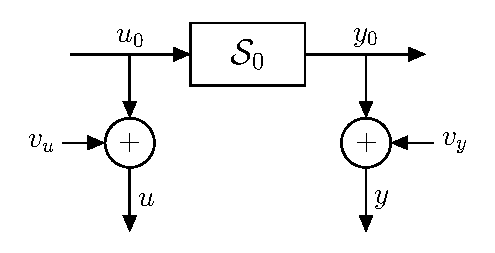
\includegraphics[width=0.5\textwidth]{Chapter2_SysIDandControl/SysIDoverview.pdf}
\caption{Generic block diagram of a system with input and output measurement noise}
\label{fig:SysIDoverview}
\end{figure}

Before considering identification or control, the nature of the system under study and its associated signals must be further clarified. There are a number of system characterizations which must be determined (or chosen), which are listed and defined below:

\begin{enumerate}
\item \textbf{Dynamic/Static:} A system which is dynamic has the property that the current output, denoted by $y(t)$, depends not only on the current input, $u(t)$, but also on past values of the input and/or output, $u(t-\tau)$ and $y(t-\tau)$ for $\tau>0$. It is equivalent to say that dynamic systems possess memory. Conversely, a static system is a memory-less system, where the current output is dependent only on the current input.
\item \textbf{Linear/Nonlinear:} A system is defined as linear if it satisfies the properties of homogeneity and additivity, i.e. the following condition is true:
\begin{align}
\mathcal{S}_0: u_1 \rightarrow y_1 \text{ and } \mathcal{S}_0: u_2 \rightarrow y_2 &\implies \mathcal{S}_0: \alpha u_1+ \beta u_2 \rightarrow \alpha y_1+ \beta y_2 \; \; \forall \alpha, \beta.
\end{align}
If this condition is not satisfied in general, the system is nonlinear.
\item \textbf{Time-invariant/Time-varying:} A time-invariant system does not change the nature of its input-output transformation over time, while for time-varying systems, the time at which a given input is applied can change the resulting output. 
\item \textbf{Discrete-time/Continuous-time:} A system which is discrete-time performs transformations using sampled input and output signals. This means that the signals $u(t)$ and $y(t)$ are defined only for specific values of $t$. When the samples are regular (evenly spaced), the argument $t$ is typically restricted to integer values to represent the sample number. Continuous-time systems, as the name suggests, consider input signals which are continuous functions and produce a corresponding continuous output signal. It is worthwhile to note that while virtually all physical systems are continuous in nature, the discrete-time framework is useful in our digital world where measurements are taken and stored as discrete samples. 
\item \textbf{SISO/MIMO:} A single-input-single-output (SISO) system possesses scalar input and output signals. Conversely, a multiple-input-multiple-output (MIMO) system may have multiple signals at the input and output ports. This means that the signals $u(t)$ and $y(t)$ at any instance of $t$ are \emph{vectors} containing multiple scalar components.
\end{enumerate}

Many of the above characterizations should be considered as mathematical approximations, rather than concrete physical properties of the system. For example, it would be fair to say that no real system is truly linear, however there are many systems for which a linear model is satisfactory in capturing the important dynamic behaviour for prediction or control purposes \cite{Pintelon2012}. Indeed, the entire pursuit of prescribing a mathematical model to a real process should be considered an abstraction from reality, since an exact description is never attainable. This philosophical perspective is eloquently presented in \cite{Ljung1987}:
\begin{quote}
``In a sense, there is an impenetrable but transparent screen between our world of mathematical descriptions and the real world. We can look through this window and compare certain aspects of the physical system with its mathematical description, but we can never establish an exact connection between them.'' \hfill (Lennart Ljung)
\end{quote} 

Nevertheless, all systems must be characterized in a mathematical sense prior to modeling. In this thesis, we will focus on SISO systems which are well approximated by a discrete-time, dynamic, nonlinear, time-invariant description.

\section{The identification process}

When it comes to the identification of a dynamical system from experimental data, there are a number of distinct steps in the process. Naturally, much of the attention in system identification literature is focussed on estimation algorithms, and how to transform the measured data into an accurate system model. However, before the estimation stage there are other considerations to be made. These considerations include the experimental procedure which should be designed in order to obtain informative data from the system, the model structure which must be chosen for estimation, and a metric which should be constructed to quantify the performance of candidate models during estimation. Even after a model estimate has been obtained, there is further work in validating the model on separate data to ensure it meets specifications for the intended use.

An overview of the full identification process is depicted in Figure \ref{fig:IdentProcess}. Note that many of the stages can be informed by prior knowledge of the system, as well as previous unsuccessful estimation attempts. The latter point highlights the iterative nature of system identification. It can be difficult to choose the experimental conditions, model class, etc. in an optimal way without yet having a mathematical system description, however those initial attempts which do not meet specifications can provide information for revising and improving the process. 

\begin{figure}[h]
\centering
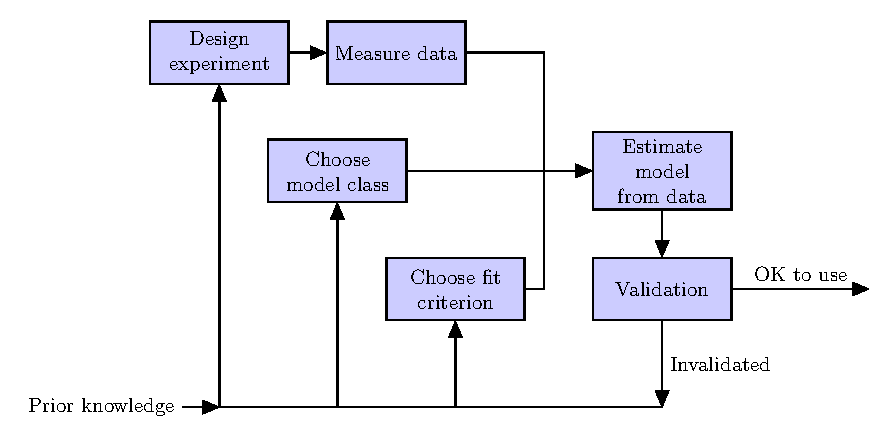
\includegraphics[width=0.9\textwidth]{Chapter2_SysIDandControl/IdentificationProcess.pdf}
\caption{An overview of the identification process}
\label{fig:IdentProcess}
\end{figure}

Background will be provided in the following subsections for each stage in the identification process. These sections will also provide some context regarding each stage in terms of this thesis.

\subsection{Experiment design} 

Broadly speaking, the objective when designing an identification experiment is to ensure that the measured data provides maximal information with respect to the intended use of the system model \cite{Gevers1986}. The experiment design should cater to any practical constraints which are present, and consider factors such as experiment duration, presence of stabilizing feedback, and most importantly, the nature of the excitation signal. Optimal input design has itself become a rich sub-field, which considers how best to choose the class of signal used for excitation, as well as its power spectrum and range \cite{Bombois2006}, \cite{Hildebrand2007}.

Experiment design is not a crucial element of this thesis. Several signal classes are used for excitation, including Gaussian white noise, pseudo-random binary sequence (PRBS), and random phase multisine. White noise and PRBS have an approximately flat power spectrum across the entire frequency band, while multisines allow precise control over the power contained at each frequency \cite{Schoukens2016}, being explicitly constructed from the sinusoid summation: 
\begin{equation}
u_0(t) = A_0 + \sum_{i=1}^{F} A_i \text{cos}(2 \pi i f_0 t + \phi_i),
\end{equation}
where $A_0$ gives the constant offset, $f_0$ is the fundamental frequency (in Hz), $F$ is the maximum harmonic excited, and $\phi_i$ are randomly selected phase shifts.

\subsection{Choosing a model class}

A plethora of model classes exist for describing dynamical systems, and a selection here has consequences for the estimation methods which can be used as well as the suitability of the estimated model for its intended use. The first choice which should be made is whether to use a parametric or nonparametric representation. While parametric models have a fixed and finite number of parameters, nonparametric models are characterized by a parameter set which is infinite in theory and in practice can grow indefinitely with increasing data length. Another crucial question is whether to construct a model in the time or frequency domain, i.e. whether to express the input to output transformation in terms of time domain or frequency domain signals.

For discrete linear systems, popular model classes include the parametric ARMAX, Box-Jenkins and state space structures, as well as the nonparametric impulse response model and its frequency domain equivalent, the frequency response function (FRF). For nonlinear systems, as discussed in Chapter \ref{chap:1}, there are a number of representations available. NARMAX and block-oriented models can be fully or partially parametric, while the Volterra series and its related expansions are nonparametric. The Volterra series also has a frequency domain equivalent formulation comprised of GFRFs. This thesis assumes a preference for nonparametric modeling, and deals with Volterra series estimation in both time and frequency domain. Other nonlinear model classes, e.g. block-oriented structures, are sometimes used to construct a simulated `true system' on which identification is performed.

When a model class has been selected, it defines a set, $\mathcal{M}$, of all possible models for the system. The set is defined as
\begin{equation}
\mathcal{M} := \{ \mathcal{S}(\theta) | \theta \in \Theta \subset \mathbb{R}^n \}
\end{equation}
where $\theta \in \mathbb{R}^n$ is a vector of parameters completely describing the model, $\Theta$ is the vector space of all possible parameter vectors, and $\mathcal{S}(\theta)$ is the parameterized system model.


\subsection{Choosing the fit criterion}

Once experimental data has been collected and a model class chosen for a system, a metric $V(\theta)$ is defined in order to differentiate the performance of model candidates in the estimation stage. This metric will be labelled the `fit criterion', which for any given $\theta$ assigns a numeric value representing how well the corresponding model fits the observed experimental data. 

The fit criterion should be chosen based on the context in which the model will be used, but care must be taken since this choice will also have implications for computational complexity in the estimation phase. Typically, the criterion $V(\theta)$ is based on some measure of distance between the measured output and the model output predicted using $\mathcal{S}(\theta)$. Alternatively (and sometimes equivalently), $V(\theta)$ can be formulated as a statistical likelihood function which provides the likelihood of seeing the observed data given a model parameterized by $\theta$ and some assumed measurement noise distributions. 

The estimation methods developed in this thesis use fit criteria which can be framed both in terms of a distance measure and a statistical function, with the relationship between the two criteria discussed in Section \ref{sec:ReLS_Chap2}.

\subsection{Model estimation}

The specific details of model estimation will depend heavily on the model structure and fit criterion which have been chosen in the previous stages. In the most general case, model estimation can be framed simply as the optimization of a criterion $V(\theta)$ over the allowable space $\Theta$. For example, if the criterion is a distance measure between the measured and predicted outputs, our model can be defined by the minimization problem:
\begin{equation}
\hat{\theta} = \text{arg } \underset{\theta}{\text{min}} \; V(\theta).
\end{equation}

Depending on the complexity of the model and fit criterion, solving the optimization problem can be as simple as an analytic solution. Conversely, $V(\theta)$ may be highly non-convex, requiring techniques that can efficiently locate a global optimum. The estimation methods in this thesis will feature minimization problems of the latter type, and the efficiency of finding solutions is addressed in Chapter \ref{chap:4}.

\subsection{Validation}

After obtaining a model estimate, it is important to test the model's prediction accuracy on a new set of experimental data, known as validation data, which is uncorrelated with the data used for estimation. This allows a user to assess whether the model meets the specifications for its intended purpose, and will also detect problems like overfitting, where some of the model parameters are inadvertently used to capture the noise in the estimation data rather than the underlying process.   

\section{The impulse response model}

The impulse response model is a foundation stone of linear systems theory. For a discrete-time SISO system, it is defined as the output response to a unit impulse applied at sample time $t=0$, i.e. $u(t) = \delta(t)$ where $\delta(t)$ denotes the discrete-time unit impulse function,
\begin{equation}
\delta(t) = \begin{cases} 1 & \text{for } t = 0 \\
0 & \text{for } t \neq 0 \end{cases}
\end{equation}

This impulse response is denoted by $h(t)$, which can be infinite in length. The infinite impulse then forms a unique description for any linear system, since the system response to any arbitrary input is just a convolution of the input with the impulse response,
\begin{equation}
\label{eq:IIRdefn}
y(t) = \sum_{\tau=-\infty}^{\infty} h(\tau) u(t-\tau) = h(t) * u(t),
\end{equation}
where $*$ is the convolution operator. It is clear that $h(t)$ represents a nonparametric model structure for linear systems, which will be denoted the infinite impulse response (IIR) model.

Models of infinite dimension are not useful in a practical setting, however there are some generic properties of a linear impulse response which are independent of the generating system, and these properties can be exploited to produce a finite-parameter model. First, we impose an assumption of causality (no system can predict the future), such that $h(t) = 0$ for $t<0$. Thus, the negative tail of the impulse can be disregarded. We will also restrict our scope to the set of stable linear systems, which brings an additional implication that the impulse response tends to 0 over time:
\begin{equation}
h(t) \xrightarrow{\: t \to \infty \:} 0.
\end{equation} 

Under these conditions, it follows that any impulse response model can be truncated to a finite length, $t= 0,1,\hdots,n-1$, where $h(n)$ is the first negligible component as dictated by some user-specified threshold. The truncation length $n$, will be referred to as the `effective memory length' of the system. The truncated impulse forms a new nonparametric description which will be denoted the finite impulse response (FIR) model, and written mathematically as, 
\begin{equation}
\label{eq:FIRdefn}
y(t) = \sum_{\tau=0}^{n-1} h(\tau) u(t-\tau).
\end{equation}
Examples of truncated impulse responses are shown in Figure \ref{fig:ImpulseExamples} for arbitrary linear systems. 

\begin{figure}[h]
\centering
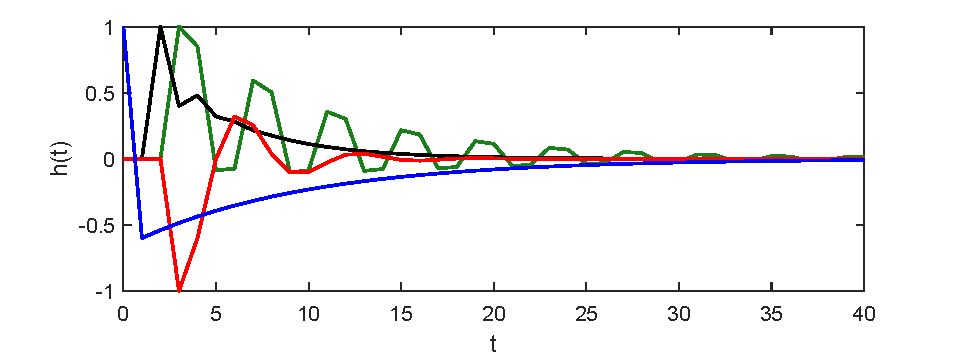
\includegraphics[width = 0.9\textwidth]{Chapter2_SysIDandControl/RandomFIRs}
\caption{Example impulse responses for randomly generated discrete linear filters}
\label{fig:ImpulseExamples}
\end{figure}

\section{Classical estimators}

For the identification of dynamical systems, it is often possible to formulate the estimation problem such that classical estimation techniques can easily be applied. An example of this is when the system model is `linear-in-the-parameters'. Assuming we have some parameter vector $\theta \in \mathbb{R}^{n}$ which is a column vector, a linear-in-the-parameters model has output response at sample $t$ given by:
\begin{equation}
\label{eq:LeastSquares_1row}
y(t) = \phi(t)^T \theta + e(t)
\end{equation}
where $T$ is the vector transpose operator. The $e(t)$ term captures any error between the measured output and model, and $\phi(t) \in \mathbb{R}^{n}$ is known as the regressor vector, which can contain any mixture of past output and input samples depending on the model structure. If we consider the FIR model from (\ref{eq:FIRdefn}), which is linear-in-the-parameters, then (\ref{eq:LeastSquares_1row}) holds with
\begin{align}
\theta &= [h(0) \; h(1) \; \hdots \; h(n-1)]^T, \label{eq:ParameterVector4Impulse} \\
\phi(t) &= [u(t) \; u(t-1) \; \hdots \; u(t-n+1)]^T.
\end{align}

While (\ref{eq:LeastSquares_1row}) explains the output response for a single sample, $t$, the representation can be extended to model an entire output data record. Assuming $N$ samples of input and output data ($t = 0, \hdots, N-1$) are measured from a system, and considering the FIR model (\ref{eq:FIRdefn}), an output vector $Y = [y(n-1) \; y(n) \; \hdots \; y(N-1)]^T$ is constructed and modeled as,
\begin{equation}
\label{eq:LeastSquares_allrows}
Y =  \Phi^T \theta + E
\end{equation}
where $E$ is a vector containing the errors $e(t)$, and $\Phi \in \mathbb{R}^{n \times (N-n+1)}$ is the regressor matrix, given by
\begin{equation}
\Phi = \begin{bmatrix} \phi(n-1) &\phi(n) &\hdots &\phi(N-1) \end{bmatrix}.
\end{equation}

\subsection{The least squares approach}

In order to estimate $\theta$ from (\ref{eq:LeastSquares_allrows}), a fit criterion $V(\theta)$ is required. The least squares (LS) approach employs a sum of squared errors between the model and the measurement as such a criterion. Mathematically, the LS criterion can be expressed as,
\begin{align}
V_{LS}(\theta) &= E^T E \\ 
&= (Y-\Phi^T \theta)^T(Y - \Phi^T \theta) \\
&= \norm{(Y-\Phi^T \theta)}_2^2,
\label{eq:LS_criterion}
\end{align}
where $\norm{\cdot}_2^2$ denotes the squared 2-norm operator. The resulting optimization problem to obtain our estimate $\hat{\theta}$, is given by
\begin{equation}
\hat{\theta} = \text{arg } \underset{\theta}{\text{min}} \; \norm{(Y-\Phi^T \theta)}_2^2,
\label{eq:LS_opt}
\end{equation}
which is easily shown to be a convex problem with the analytic solution,
\begin{equation}
\hat{\theta} = (\Phi \Phi^T)^{-1}(\Phi Y).
\label{eq:LS_analytic}
\end{equation}

For the least squares approach, the interpretation of `error' is quite general. it can represent output measurement noise, or model errors due to a mismatch between the model and true system, or a combination of both. Of course, the true source of these errors will have an effect on the properties of the least squares estimator, however before discussing this, the maximum likelihood estimator will be derived for our linear-in-the-parameters structure.

\subsection{Maximum likelihood estimation}

In maximum likelihood estimation (MLE), our fit criterion is chosen as the likelihood function, $\mathcal{L}(Y;\theta)$, which gives the likelihood of observing the output vector $Y$ given some model structure parameterized by $\theta$. In order to express the likelihood analytically, the system model should have some statistical properties imposed, and in particular for our linear-in-the-parameters representation (\ref{eq:LeastSquares_allrows}), the stochastic behaviour of the error vector $E$ should be defined.

One common assumption for $E$, and the one which will be discussed here, is that $E$ is a vector of independent and identically distributed (i.i.d.) random variables each with a zero mean normal distribution. Observing Figure \ref{fig:SysIDoverview}, this assumption implies that we have Gaussian white measurement noise at the output ($v_y(t) = e(t)$), and no input noise ($v_u = 0$). This produces a stochastic model description for $Y$, i.e.
\begin{equation}
Y \sim \mathcal{N}(\Phi^T \theta,\sigma^2 I),
\end{equation}
where $\sigma^2$ is the variance of the errors in $E$, and $I$ is an identity matrix of appropriate size. An analytic expression for the likelihood, and thus the fit criterion, can be written using the multivariate normal distribution, yielding
\begin{equation}
V_{ML}(\theta) = (2 \pi \sigma^2)^{-\frac{N-n+1}{2}} \text{exp}\bigg( -\frac{1}{2 \sigma^2} \norm{(Y-\Phi^T \theta)}_2^2 \bigg).
\label{eq:ML_criterion}
\end{equation}
The optimization problem for estimating $\theta$ is simply to maximize the likelihood function,
\begin{equation}
\hat{\theta} = \text{arg } \underset{\theta}{\text{max}} \; V_{ML}(\theta).
\label{eq:ML_opt}
\end{equation}

It is trivial to show that under the assumption above on the error, and substituting (\ref{eq:ML_criterion}) into (\ref{eq:ML_opt}), the problem will reduce to (\ref{eq:LS_opt}). Thus the maximum likelihood approach shares the same analytic solution (\ref{eq:LS_analytic}) as the least squares approach for this case. This explains the popularity of the Gaussian measurement noise assumption in MLE, since it produces a familiar analytic solution. However, the estimator performance will degrade if there is significant input measurement noise, or the output noise is a correlated (non-white) sequence. In these circumstances, a more complex stochastic model may be required.

\subsection{Estimator properties}

\begin{defn}[Estimator]
For a model set $\mathcal{M}$, an estimator is an operator which maps the measured data $u$ and $y$ to a parameter vector estimate $\hat{\theta}$. 
\end{defn}
To analyze the properties of an estimator, the philosophical truth that real systems can never be fully described by abstract models will be abandoned out of necessity, and replaced with the pretence that there exists a true \emph{mathematical} description of the system, $\mathcal{S}_0$. Under the further condition that this true system lies within our model set, i.e. $\mathcal{S}_0 \in \mathcal{M}$, the notion of a true parameter vector can be introduced.
\begin{defn}[True parameters]
The true parameter vector, $\theta_0$, is a vector satisfying $\mathcal{S}(\theta_0) = \mathcal{S}_0$.
\end{defn}

Any estimate $\hat{\theta}$ produced by an estimator is a function of input and output measurements obtained from the system, which contain stochastic noise in general. The estimate itself should therefore be treated as a random variable, and it is the statistical properties of this variable which define the performance of the estimation method. There are three properties in particular which, when combined, provide an appreciation of the performance of the estimator. They are the bias, covariance and mean square error (MSE).

\begin{defn}[Bias]
The bias of an estimator is the difference between the expected value of the estimate and the true parameters:
\begin{equation}
\Bias(\hat{\theta}) = \textbf{E}\{ \hat{\theta} \} - \theta_0.
\end{equation}
An unbiased estimator is one for which $\textbf{E}\{ \hat{\theta} \} = \theta_0$.
\end{defn}

\begin{defn}[Covariance]
The covariance of an estimator is its variability or dispersion around the expected value, described by:
\begin{equation}
\Cov(\hat{\theta}) =  \textbf{E} \bigg\{ \big( \hat{\theta} - \textbf{E}\{ \hat{\theta} \} \big) \big( \hat{\theta} - \textbf{E}\{ \hat{\theta} \} \big)^T \bigg\}.
\end{equation}
\end{defn}

\begin{defn}[MSE]
The MSE of an estimator combines the effects of bias and covariance into a total error metric, given by:
\begin{align}
\MSE(\hat{\theta}) &=  \textbf{E} \bigg\{ \big( \hat{\theta} - \theta_0 \big) \big( \hat{\theta} - \theta_0 \big)^T \bigg\} \\
&= \Bias(\hat{\theta}) \Bias(\hat{\theta})^T + \Cov(\hat{\theta}).
\end{align}
\end{defn}

Observing these three properties, it is clear that an accurate estimator should have the lowest possible bias and covariance (in the matrix sense) in order to minimize its MSE. It would seem natural then, to consider only unbiased estimators such that $\text{Bias}(\hat{\theta}) = 0$. Indeed, the LS and MLE estimators, (\ref{eq:LS_opt}) and (\ref{eq:ML_opt}), will be unbiased under the following conditions:
\begin{enumerate}
\item $\mathcal{S}_0 \in \mathcal{M}$
\item No input measurement noise
\item The output error $E$ is any zero mean stochastic process
\end{enumerate}
Note that in the MLE case, the Gaussian i.i.d. noise assumption need not be met to ensure unbiasedness. Covariance, on the other hand, will reduce further under the correct noise distribution. There is a fundamental restriction on how far the covariance can decrease in unbiased estimators, and this is known as the Cramér-Rao lower bound \cite{Pintelon2012}. An unbiased estimator with covariance obtaining the lower bound is called an \emph{efficient} estimator. 

When considering models which require many parameters, such as the nonparametric impulse response, the Cramér-Rao lower bound can present a problem. For example, when the number of samples $N$ used in the estimation is low, or measurement noise is significant, even an efficient estimator will have very high covariance and hence is likely to produce an inaccurate model. In these cases, it can be beneficial to introduce a small bias into the estimator in such a way that the covariance reduces dramatically along with the MSE. Typically, this bias reflects some prior belief on how the parameter vector should behave, and can be introduced by adding an additional penalty to the fit criterion (known as `regularization'), or by adopting a Bayesian estimation approach. These two techniques are intrinsically related and will form the core of all identification methods presented in this thesis.

\section{Regularized least squares and the Bayesian {perspective}}
\label{sec:ReLS_Chap2}

The least squares approach to model estimation is attractive due to its simplicity, with an analytic solution guaranteed for any model structure that is linear-in-the-parameters as long there is enough measurement data available. In practice however, and particularly for nonparametric structures such as the FIR model, estimation using least squares will lead to poor results under many circumstances. The issues relevant to FIR estimation are:
\begin{itemize}
\item The estimator will have large covariance if the number of data points $N$ does not greatly exceed the number of parameters, $n$.
\item The estimator will have large covariance when output measurement noise is significant.
\item The estimation problem will be ill-conditioned if the input excitation is not sufficiently exciting.
\item The estimation problem does not have a unique solution when $N < 2n-1$.  
\end{itemize} 
Observing these issues, it is clear that a long, well designed and relatively noise-free experiment is required to achieve good impulse response estimates, particularly when the impulse has a large effective memory length, $n$. There are many practical identification settings where such ideal experimental conditions are not possible, and consequently will require more advanced estimation techniques. 

As an example, FIR model estimates are obtained for a simulated linear system using least squares on two sets of experimental data, where each experiment has Gaussian excitation $u(t) \sim \mathcal{N}(0,1)$ and Gaussian measurement noise $e(t) \sim \mathcal{N}(0,\sigma^2)$.  The first experiment records $N=2000$ data samples and $\sigma^2$ is chosen such that the Signal-to-Noise Ratio (SNR)\footnote{SNR is defined using the variance ratio: SNR = $\Var [y_0]/\Var [e]$} is 40dB. The second experiment records only $N=200$ samples with a decreased SNR of 20dB. The least squares estimated impulse response for each experiment is plotted in the left half of Figure \ref{fig:ExampleImpulseEsts}, along with the true system, showing the performance degradation that comes with small data lengths and high noise levels. The right half of Figure \ref{fig:ExampleImpulseEsts} plots \emph{regularized} estimates for the same experiments, which are seen to be far less sensitive to decreases in data length and SNR. The mathematical techniques for performing regularized FIR estimation will now be discussed.

\begin{figure}[h]
\centering
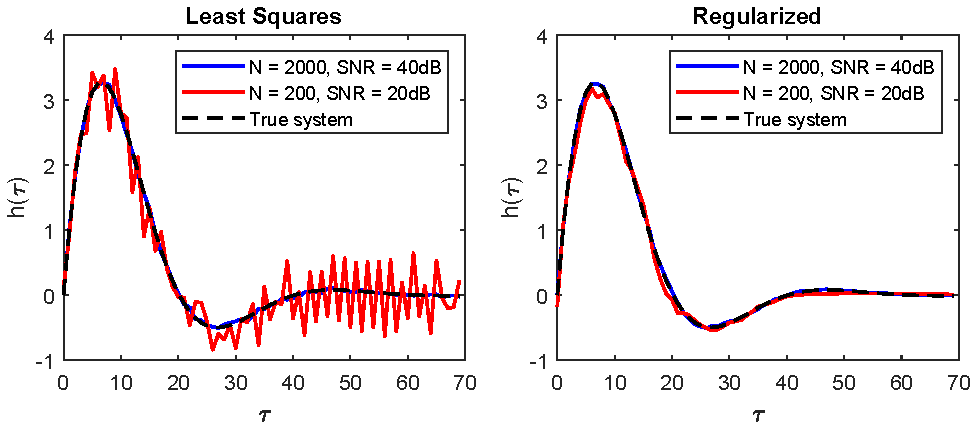
\includegraphics[width = 0.98\textwidth]{Chapter2_SysIDandControl/LS_example2}
\caption{Least squares (left) and regularized (right) FIR estimates for an example linear system using different data lengths and SNRs}
\label{fig:ExampleImpulseEsts}
\end{figure}

\subsection{Regularization penalty options}

In its most general form, regularization can be described as the inclusion of an additional term in the fit criterion of an estimator. The regularized least squares (ReLS) criterion is then given by,
\begin{equation}
V_{ReLS}(\theta) = \norm{(Y-\Phi^T \theta)}_2^2 + T(\theta),
\end{equation} 
where $T(\theta)$ is an additional penalty term acting directly on the parameter vector. Such an addition can be used to impose certain expected behaviours on the estimated parameter vector, thereby reducing the effect of noisy measurements and improving the estimation accuracy. In ill-posed estimation problems, the added penalty can also improve conditioning.

Various forms have been proposed for $T$, starting with the early results of Tikhonov \cite{Tikhonov1963}, for which the term `Tikhonov regularization' was coined. The penalty for this type of regularization takes the general form:
\begin{equation}
T(\theta) = \norm{\Gamma \theta}_2^2,
\label{eq:TikhonovPenalty}
\end{equation}  
where $\Gamma$ is a Tikhonov matrix chosen to impose certain parameter behaviours. When the Tikhonov matrix is chosen as a multiple of the identity matrix, i.e.
\begin{equation}
T(\theta) = \gamma \norm{\theta}_2^2,
\end{equation}
for some $\gamma \in \mathbb{R}^+$, then the regularization method is known within the statistics community by the term `ridge regression' \cite{Hoerl1970}. This scheme is particularly useful for parameter vectors which are expected to be sparse, since parameters are heavily penalized for being too far from zero. If the parameters in $\theta$ have different physical units, appropriate pre-scaling should be applied.   

A more recent proposal for regularized estimation of sparse parameter vectors is the lasso (Least Absolute Shrinkage and Selection Operator) algorithm \cite{Tibshirani1996}, which replaces the 2-norm penalty with a 1-norm, giving
\begin{equation}
T(\theta) = \gamma \norm{\theta}_1.
\end{equation}
The lasso approach has been shown to exhibit some nice properties with respect to capturing the set of zero elements in the true parameter vector, $\theta_0$ \cite{Tropp2006}. 

Yet another similar technique is nuclear norm regularization \cite{Fazel2001}, \cite{Mohan2010}, which uses penalty term
\begin{equation}
T(\theta) = \gamma \norm{H(\theta)}_*,
\end{equation}
with $H(\theta)$ denoting the Hankel matrix of $\theta$, and $\norm{\cdot}_*$ being the nuclear norm operator, defined as the sum of singular values of its matrix argument. The nuclear norm has been shown to be a convex approximation of the matrix rank function \cite{Fazel2001}, and for $\theta$ given by an impulse response model (as in (\ref{eq:ParameterVector4Impulse})), penalizing the Hankel matrix rank is equivalent to penalizing the order (i.e. complexity) of the linear system.

\subsection{The quadratic penalty}

One penalty term in particular has garnered a significant amount of attention in recent decades, first in the machine learning field for function estimation \cite{Rasmussen2006}, before being introduced to the system identification community as a method of low covariance impulse response estimation \cite{Pillonetto2010}. The penalty is quadratic in nature, having the form,
\begin{equation}
T(\theta) = \gamma \theta^T P^{-1} \theta.
\label{eq:QuadraticPenaltyT}
\end{equation}
Comparison with (\ref{eq:TikhonovPenalty}) reveals this term to be just a special case of Tikhonov regularization, where $\gamma P^{-1} = \Gamma^T \Gamma$. 

The total regularized estimation problem with the quadratic penalty (\ref{eq:QuadraticPenaltyT}) can be stated as
\begin{equation}
\hat{\theta} = \text{arg } \underset{\theta}{\text{min}} \norm{(Y-\Phi^T \theta)}_2^2 + \gamma \theta^T P^{-1} \theta,
\label{eq:Estimator_QuadraticPenalty}
\end{equation} 
which is a convex problem with an analytic solution,
\begin{equation}
\hat{\theta} = (P \Phi \Phi^T + \gamma I)^{-1} P \Phi Y.
\label{eq:QuadraticPenalty_analyticsolution}
\end{equation} 
The terms $\gamma$ and $P$ are tunable, with $P$ enforcing certain behaviours in the estimated parameter vector and $\gamma$ scaling the effect of the regularization, much like generic Tikhonov regularization. It is the specific techniques for designing and tuning these terms, however, which has recently received an explosion of interest \cite{Pillonetto2014}. To understand how these techniques emerged, it is important to first look at the MSE property of our regularized estimator (\ref{eq:QuadraticPenalty_analyticsolution}).

It will be assumed that we have the linear-in-the-parameters model (\ref{eq:LeastSquares_allrows}) with true parameter vector $\theta_0$, and i.i.d. errors such that $\mathbf{E} \{ EE^T \} = \sigma^2 I$. Under these conditions, it can be shown that the MSE of (\ref{eq:QuadraticPenalty_analyticsolution}) is minimized (in the matrix sense) by the following choices \cite{Chen2012}:
\begin{align}
\gamma &= \sigma^2, \\
P &= \theta_0 \theta_0^T. \label{eq:OptimalMSE_P}
\end{align}
It is clear that an optimal choice of $P$ relies on knowing the true parameter vector, a fact which is not particularly useful in an estimation setting. The form of (\ref{eq:OptimalMSE_P}) does, however, lead to two useful mathematical interpretations for tuning $P$. 

The first method interprets $P$ as the reproducing kernel of a Hilbert space containing all allowable model parameterizations (see e.g. \cite{Scholkopf2001}), and in this context the estimation process is labelled `kernel-based regularization'. The second method, and the one which will be adopted in this thesis, is a Bayesian interpretation of $\theta_0$ and therefore $P$. If instead of viewing the system as deterministic, $\theta_0$ is expressed as a random variable with some covariance $\mathbf{E} \{ \theta_0 \theta_0^T\} = \Pi$, then (\ref{eq:OptimalMSE_P}) can be replaced with $P = \Pi$. Tuning of the covariance can then be performed via established Bayesian methods, hence this form of regularization is often termed Bayesian regularization, or Gaussian Process Regression (GPR) when normal distributions are employed.

\subsection{Bayesian interpretation}

Having established that a Bayesian perspective may be useful in the regularized least squares problem (\ref{eq:Estimator_QuadraticPenalty}), the problem can be reframed as a Bayesian estimation problem. In doing so, the first step is typically to reinterpret the true parameter vector $\theta_0$ as a zero mean Gaussian process:
\begin{equation}
\theta_0 \sim \mathcal{N}(0,P).
\end{equation}
As is the case for Bayesian estimation in general, this assumption does not indicate that the physical system is truly stochastic in nature. Rather, it is a convenient mathematical abstraction which can be used to express our prior belief on how the system should behave. It is for this reason that $P$ will be labelled the \emph{prior covariance} matrix. 

When the system is represented by a FIR model structure, there are two behaviours in particular which are encoded into the Gaussian covariance, $P$:
\begin{enumerate}
\item The impulse response decays exponentially towards zero over time.
\item The impulse response is a smooth function.
\end{enumerate} 
The decay behaviour can be represented by an exponential decrease in parameter variance along the diagonal of $P$, while smoothness is induced by increasing the off-diagonal correlation components of parameters which are in close proximity to each other. Several covariance structures of varying complexity have been proposed in the literature to capture such behaviour \cite{Pillonetto2010}, \cite{Chen2011}, where the two most typical choices are, \\ \\
\textbf{Tuned/Correlated (TC): }
\begin{equation}
\begin{split}
\label{eq:TCstructure}
&P(x,y) = c \lambda^{\max(x,y)}, \\
&c \geq 0, \; 0 \leq \lambda < 1, \; \eta_P = [c,\lambda].
\end{split}
\end{equation}
\textbf{Diagonal/Correlated (DC):}
\begin{equation}
\begin{split}
\label{eq:DCstructure}
&P(x,y) = c \lambda^{(x+y)/2} \rho^{|x-y|}, \\
&c \geq 0, \; 0 \leq \lambda < 1, \; |\rho| \leq 1, \; \eta_P = [c,\lambda, \rho].
\end{split}
\end{equation}
In the expressions (\ref{eq:TCstructure}) and (\ref{eq:DCstructure}), $P(x,y)$ denotes the $x,y$\textsuperscript{th} element of $P$, and $\eta_P$ is a vector containing all tunable hyperparameters for the covariance matrix.

Considering once again the linear-in-the-parameters structure (\ref{eq:LeastSquares_allrows}), the error vector $E$ is assumed, for mathematical convenience, to be white Gaussian measurement noise, i.e. $E \sim \mathcal{N}(0,\sigma^2 I)$. The result is a fully Gaussian framework where the joint distribution of the output and parameter vector can be easily found as,
\begin{equation}
\begin{bmatrix}
\theta \\ 
Y
\end{bmatrix} \sim \mathcal{N} \Bigg(
\begin{bmatrix}
0\\ 
0
\end{bmatrix},
\begin{bmatrix}
P & P \Phi\\ 
\Phi^T P & \Phi^T P \Phi + \sigma^2 I 
\end{bmatrix} \Bigg).
\label{eq:thetaY_jointdistribution}
\end{equation}

Assuming for the moment that $P$ is known, producing an estimate for $\theta$ via the Bayesian approach requires a posterior distribution conditioned on the observed data, $p(\theta|Y)$. Forming conditional distributions for jointly Gaussian variables is a well-established practice which yields the following normal posterior,
\begin{equation}
p(\theta|Y) \sim \mathcal{N} \Bigg( (P \Phi \Phi^T + \sigma^2 I)^{-1} P \Phi Y, P - P \Phi (\Phi^T P \Phi + \sigma^2 I)^{-1} \Phi^T P \Bigg)
\end{equation}
The maximum a posteriori (MAP) estimate for $\theta$, conditioned on $Y$, is simply the mean of the distribution,
\begin{equation}
\hat{\theta} = (P \Phi \Phi^T + \sigma^2 I)^{-1} P \Phi Y,
\label{eq:MLE_BayesianRegularization}
\end{equation}
which is identical to the regularized least squares solution (\ref{eq:QuadraticPenalty_analyticsolution}) with $\gamma = \sigma^2$. Thus, a fully Bayesian approach provides the same analytic solution as quadratically penalized least squares. 

We can now proceed one step further and take advantage of our Bayesian framework to tackle the problem of appropriately tuning $P$. Noting that the noise variance, $\sigma^2$, is also typically unknown, the most common method is to collect all tunable hyperparameters into a single vector $\eta = [\eta_P, \; \sigma^2]$ and consider the marginal likelihood, $\mathcal{L}(Y;\eta)$, where $\theta$ has been marginalized out:
\begin{equation}
\mathcal{L}(Y;\eta) \sim \mathcal{N}(0, \Sigma_Y(\eta)),
\label{eq:MarginalLikelihoodDist_eta}
\end{equation}
where $\Sigma_Y(\eta) = \Phi^T P(\eta_P) \Phi + \sigma^2 I $ from (\ref{eq:thetaY_jointdistribution}). By maximizing the marginal likelihood function, hyperparameters can be tuned purely on the observed system data, a technique known as empirical Bayes. 

Maximizing (\ref{eq:MarginalLikelihoodDist_eta}) reduces to the minimization problem,
\begin{equation}
\hat{\eta} = \text{arg } \underset{\eta}{\text{min }} Y^T \Sigma_Y^{-1} Y + \text{log det } \Sigma_Y,
\label{eq:MarginalLikelihood_opt}
\end{equation}
which is in general a non-convex optimization problem with multiple local minima \cite{Rasmussen2006}. Methods to improve robustness and computation time have been explored in the literature, in particular by employing QR factorization to avoid the inversion of large matrices \cite{Chen2013}. Once $\eta$ has been tuned, the model estimate $\hat{\theta}$ follows immediately via (\ref{eq:MLE_BayesianRegularization}).

\section{Model-based control}

The field of control has a long and interesting history spanning back to ancient times, however the development of modern control theory began in the 20th century. In particular, the World War era and subsequent space race provided the catalyst for rapid advancements in our understanding of feedback control \cite{Goodwin2001}. To effectively design and analyze feedback control architectures, mathematical models of the dynamical systems were required, and so the fields of system identification and control evolved in closely related trajectories.

While model-based feedback controllers are now ubiquitous in everything from manufacturing and transport to telecommunications and finance, there are still applications where such control schemes are difficult or impossible to implement effectively. For example, control problems which involve strong nonlinear dynamics, large numbers of inputs and outputs, or complex constraints are not well suited to traditional feedback control. In the process industries, where such complexities are common, the Model Predictive Control (MPC) approach emerged, and has since received an explosion of academic interest \cite{Camacho1999}. In this thesis, we consider model-based control from the perspective of Volterra series modeling, where the nonlinear dynamics may be arbitrarily dominant. Thus, the MPC framework will be utilized to achieve efficient Volterra series model-based control.

\subsection{MPC formulation}

There are a large number of MPC variations which have been developed in the literature, all with different benefits and intended application areas. These variations fall into several broad categories including explicit, robust and stochastic MPC. In this section, a simple generalized formulation will be introduced which is sufficient for tackling the Volterra series control problem in Part \ref{part:MPC} of this thesis.

Consider a time-invariant discrete-time dynamical system which can be described by the state space equations,
\begin{align}
x(t+1) &= f \big( x(t),u(t) \big), \label{eqn:GeneralStateEqn} \\
y(t) &= g \big( x(t) \big), \label{eqn:GeneralOutputEqn}
\end{align}
where $x(t)$ is a vector of internal states at sample $t$, $u(t)$ and $y(t)$ are the system input and output respectively, $f$ is a function describing the state evolution, and $g$ is a static function mapping the states to the output. Equation (\ref{eqn:GeneralStateEqn}) is known as the \emph{state equation}, while (\ref{eqn:GeneralOutputEqn}) is labelled the \emph{output equation}. The functions $f$ and $g$ can be nonlinear in general, as will be the case in this thesis.

The typical control objective is considered, i.e. for the output to track a desired reference signal, $r(t)$. In MPC, such an objective is achieved through the use of a cost function which is repeatedly optimized over a finite receding prediction horizon. 

Suppose that some penalty function has been designed to describe the desired behaviour of the input and output signals, $\ell(y(t),u(t),r(t)) = \ell(g(x(t)),u(t),r(t))$, in a given sample. Looking first at the sample time $t=0$, the MPC optimization problem for this case can be written as,
\begin{align}
u^* = &\text{arg } \underset{u(\cdot)}{\text{min }} \sum_{t=1}^{p} \ell(y(t)|x(0),u(t),r(t)) \label{eqn:GeneralMPCOpt} \\
& \ \textrm{subject to } y(t) = g(x(t)), x(t+1) = f(x(t),u(t)), \nonumber \\
& \ \ \ u(t) = u(t-1) \ \forall t>\mu, u(t) \in \mathcal{U} \ \forall t, x(t) \in \mathcal{X} \ \forall t. \nonumber
\end{align} 
The optimal control sequence, $u^*$, is found by minimizing a sum of model-predicted penalty functions, $\ell$, over the prediction horizon, $p$. Some additional constraints may also be present, for example there may be a move horizon $\mu<p$ after which the input remains constant until the end of the prediction horizon. The input and states may also be constrained to some allowable subsets, $\mathcal{U}$ and $\mathcal{X}$, of their total vector space. Note that the initial states, $x(0)$, are assumed known here, such that robust MPC principles are not required.

Following the MPC optimization in (\ref{eqn:GeneralMPCOpt}), only the \emph{first} input in the optimal sequence, $u^*(1)$, is applied to the system. Then, at the next sample time, $t=1$, the prediction horizon recedes to sample $p+1$, and the same optimization procedure is repeated to find a new optimal control sequence. Once again, only the first value of this optimal sequence is applied, and the process continues ad infinitum. Since the optimization at any sample time $t$ is performed identically to the case in (\ref{eqn:GeneralMPCOpt}), we can assume without loss of generality that $t=0$ at every sample time, and use (\ref{eqn:GeneralMPCOpt}) to compute the next input sequence. A diagram is provided in Figure \ref{fig:MPCoverview} to illustrate the optimization process occurring at any given sample time.

\begin{figure}[h]
\centering
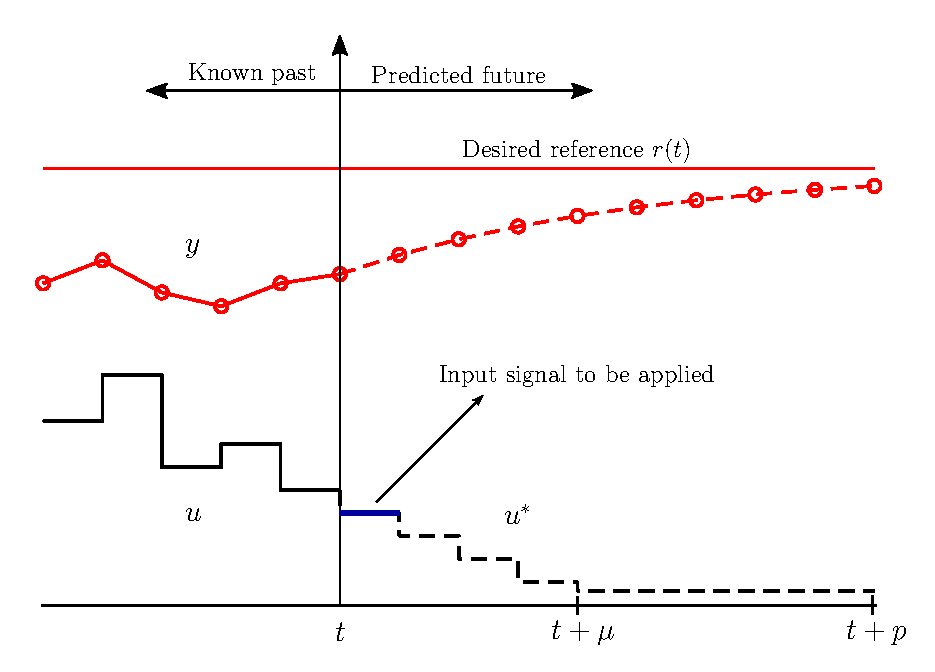
\includegraphics[width = 0.95\textwidth]{Chapter2_SysIDandControl/MPCoverview.pdf}
\caption{A visual example of the MPC optimization problem at sample time $t$. The optimal input sequence is restricted to a move horizon, $\mu$, and the corresponding model-predicted output is also shown.}
\label{fig:MPCoverview}
\end{figure}

\subsection{MPC stability}

Stability is a crucial property in control system design. Generically, and assuming a constant reference $r(t) = r$, a stable control system is one in which the output can be \emph{guaranteed} to remain bounded for all time. For a complete definition of stability, there are sometimes more subtle considerations to be made, for example the internal states of the system should also remain bounded, as well as the control input.

In the earliest days of MPC implementation, the stability of the algorithms was not well understood. While there is certainly a strong relationship between MPC and the more classical feedback control concepts of infinite horizon control and dynamic programming, the now finite horizon and input/state constraints add to the complexity of theoretical analysis \cite{Mayne2000}.

For the simplest case of unconstrained linear MPC, it is sometimes possible to construct an explicit feedback control law from the receding horizon optimization in (\ref{eqn:GeneralMPCOpt}). Thus, stability can be assessed in the same way as for traditional feedback control, by performing an eigenvalue analysis of the linear dynamic state equation in (\ref{eqn:GeneralStateEqn}). For all other cases, stability arguments can be made using the \emph{optimal value function},
\begin{equation}
V_p \big( x(0) \big) = \underset{u(\cdot)}{\text{min }} \sum_{t=1}^{p} \ell(y(t)|x(0),u(t),r(t)). \label{eqn:GeneralOptValue}
\end{equation}
One common approach is to prove that, $\forall x(0) \in \mathcal{X}$, the optimal value function monotonically decreases with each iteration. The receding horizon nature of the problem implies that it is sufficient to show the decrease in any one iteration, i.e.
\begin{equation}
V_p \big( f(x(0),u^*(1)) \big) \leq V_p \big( x(0) \big).
\end{equation}
If such a condition is satisfied, and the penalty function $\ell(y(t),u(t),r(t))$ is positive definite and equal to zero only at the desired input/output setpoint, then stability can be easily shown \cite{Mayne2000},\cite{Grune2011}.

\section{Summary}

Some fundamental concepts in system identification and control were presented in this chapter. The notion of a dynamical system was introduced, and the various stages involved in identifying such systems were discussed. Particular focus was given to the nonparametric impulse response model, which is used to motivate the advantages and drawbacks of common estimation methods such as least squares and maximum likelihood. Some popular regularization techniques were described, with an extensive coverage of quadratically penalized least squares as seen from a Bayesian perspective, which will feature prominently throughout the thesis. Finally, a generic model predictive control formulation was outlined for use in the final part of this thesis.

Many of the concepts introduced in this chapter will be extended in Chapter \ref{chap:3}, where the linear impulse response model is generalized to higher dimensions to produce the Volterra series model. In particular, a method for extending the Bayesian regularization method to Volterra series terms will be explained.

\cleardoublepage
\chapter{The Volterra Series}
\label{chap:3}
\emph{This chapter introduces the Volterra series model for nonlinear dynamical systems. Time and frequency domain representations are defined for the discrete-time case, where some assumptions and properties are also stated. Previous contributions to the Volterra series identification problem are summarized, with a comprehensive explanation of the regularized estimation method as extended from linear identification literature.}
\newpage
\section{Introduction}

For linear time-invariant systems, the nonparametric impulse response model gives a complete and intuitive description of the system space. As a consequence, its truncated FIR form is the model structure of choice in many modern regularized estimation procedures, which were discussed in Chapter \ref{chap:2}. When broadening our scope to \emph{nonlinear} time-invariant systems, an analogous nonparametric representation is known as the Volterra series \cite{Schetzen1980}, named for mathematician Vito Volterra and his pioneering work on analytic functionals \cite{Volterra1930}. 

In much the same way that linear functions are just one term in the Taylor series description of nonlinear static functions, the linear impulse response becomes one term in a series of multi-dimensional impulse responses, which together form the Volterra series description of nonlinear dynamical systems. Each successive term in the series contains one additional dimension in its impulse response, and represents a single `nonlinear order' of the system. For example, the next term after the linear impulse is a 2-dimensional impulse response which describes all 2\textsuperscript{nd} order (quadratic) nonlinear behaviour in the system. In theory, the Volterra series has both infinite terms and infinite memory lengths within each term. The series is typically defined in the time domain, since this is the domain of an impulse response, however there are also equivalent frequency domain representations \cite{Schetzen1980}, \cite{Lang2005}, \cite{Lang2007} which can be obtained using appropriate Fourier transformations. Furthermore, all representations of the Volterra series can be described using continuous- or discrete-time models.

In practice, for data-driven modeling and control, the Volterra series must be truncated such that there is a finite maximum nonlinear order, and each impulse response term has finite memory length. It has been shown in \cite{Boyd1985} that a truncated, finite memory Volterra series model can approximate any fading memory nonlinear system arbitrarily well. The fading memory condition is somewhat similar to a stability condition in linear systems, requiring that the current system output not be influenced by input signals applied in the remote past. This will also exclude nonlinear system classes which exhibit, for example, hysteresis or non-unique steady-states. The fading memory condition still leaves an incredibly broad set of systems which can be universally approximated, along with many systems which can be approximated locally within a small region of some stable equilibrium point.

The extreme versatility of Volterra series models in representing nonlinear systems will motivate the use of such models in this thesis. In particular, the identification of nonlinear systems can be performed with very little prior knowledge, requiring user selections only for the maximum nonlinear order and memory lengths. Due to the multidimensional nature of the series, however, the model requires large numbers of parameters to be estimated, and this number grows rapidly with memory length and series order. From an identification perspective, large numbers of parameters means high covariance and MSE in the resulting estimates, particularly when the input/output data length is low or measurement noise is significant. There are also implications on the computational and memory requirements when considering a large parameter space. Such complications have historically restricted the use of classical estimators on Volterra series, and only in the most recent decades have new techniques emerged which enable more widespread use of the series in data-driven modeling. Some of these techniques will be discussed in Sections \ref{sec:VolterraID_History} and \ref{sec:RegVolterraTD}. 

\section{Discrete-time representations}
\label{sec:DTrepresentations_Volterra}

While the continuous-time Volterra series is a useful concept in systems theory, the nature of sampled data and nonparametric estimation dictates that we use discrete-time models for estimation and control. In the case where the system is excited by a piecewise constant input over the sampling periods, an explicit relationship between the discrete- and continuous-time models can be established \cite{Middleton1990}. Thus, we will restrict our focus in this thesis to the discrete-time definitions of Volterra series and its related expansions. Essentially, the only difference between these definitions and their continuous-time equivalents found in e.g. \cite{Schetzen1980} is the use of summations in place of continuous integrals. Naturally, the series terms also change from being continuously defined, to being defined only at integer values of their input arguments. The time and frequency domain representations are defined below.

\subsection{Time domain representation}

The Volterra series is most often expressed in the time domain, where its discrete-time representation can be given as,
\begin{align}
y^0(t) &= h_0 + \sum_{m=1}^M y_m(t), \label{eq:VolterraTimeDomainOutput} \\
y_m(t) &= \sum_{\tau_1 = 0}^{n_m-1} \hdots \sum_{\tau_m=0}^{n_m-1} h_m(\tau_1, \hdots, \tau_m) \prod_{\tau=\tau_1}^{\tau_m} u(t-\tau), \label{eq:VolterraConvolutionDefn}
\end{align}
where $u(t)$ and $y^0(t)$ denote the true system input and output respectively, $h_0 \in \mathbb{R}$ is a constant offset, and $y_m(t)$ is the output contribution from the $m$\textsuperscript{th} nonlinear order, up to some maximum series order, $M$. These output contributions are formed via the $m$-dimensional convolution in (\ref{eq:VolterraConvolutionDefn}), where $h_m(\tau_1, \hdots, \tau_m)$ is the $m$\textsuperscript{th} term of the Volterra series, $\tau_i$ is the $i$\textsuperscript{th} lag variable for the term, and $n_m$ is its memory length.

The series terms, $h_m$, are commonly referred to as \emph{Volterra kernels}, where the $m$\textsuperscript{th} kernel is an $m$-dimensional impulse response. It is these kernels which must be estimated for a Volterra series model. It should be noted that the 1\textsuperscript{st} order contribution, $y_1(t)$, is nothing more than the FIR model from (\ref{eq:FIRdefn}), and the corresponding Volterra kernel $h_1(\tau_1)$ behaves like a linear impulse response. 

A visual depiction of the time domain series is provided in Figure \ref{fig:VolterraSeriesVisualised} for the first four terms, showing the increase in dimension and complexity with each successive kernel.

\begin{figure}[h]
\centering
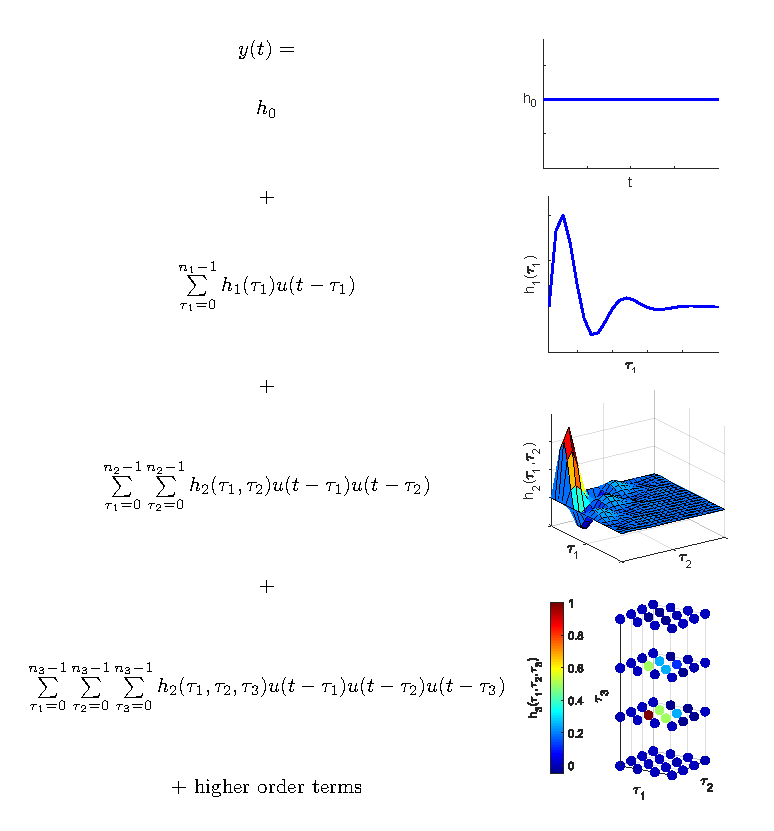
\includegraphics[width=0.9\textwidth]{Chapter3_VolterraSeries/PictorialSeries.pdf}
\caption{A visual example of the Volterra series for the first four terms}
\label{fig:VolterraSeriesVisualised}
\end{figure}

\subsection{Frequency domain representations}

The Volterra series can also be expressed in the frequency domain, with a number of competing representations available in the literature \cite{Cheng2017}. In their discrete-time form, all of these representations require an assumption that the system is in steady state. The assumption implies that an $N$-periodic (i.e. periodic with period $N$) input signal has been applied for a sufficiently long time so that the output is also $N$-periodic and free of transients. Then, for some $N$-sample measurement window, we can express the system input and output spectra, $U(k)$ and $Y^0(k)$ for $k=0,1,\hdots,N-1$, as the Discrete Fourier Transform (DFT) of their corresponding $N$-sample time domain signals $u(t)$ and $y^0(t)$. The relationship between these two steady state spectra will constitute the frequency domain model.

While each frequency domain structure has its own unique benefits, the most natural extension from the time domain series is a Generalized Frequency Response Function (GFRF) model. First derived in \cite{George1959}, the GFRF model is obtained via multidimensional Fourier transforms on each time domain series term. In discrete-time, the mathematical description is given by,
\begin{equation}
\begin{split}
Y^0(k) &= H_0(k) + \sum_{m=1}^{M} Y_m(k),  \\
Y_m(k) &= \frac{1}{N^{m-1}} \sum_{k_1 + \hdots + k_m = k} H_m(k_1, \hdots,k_m) \prod_{i=1}^{m} U(k_i), 
\end{split}
\label{eqn:GFRFoutputeqn}
\end{equation}
where $H_0(k) = h_0 \delta(k)$ is a zero frequency component from the constant offset $h_0$, $H_m(k_1, \hdots,k_m)$ is the $m$\textsuperscript{th} order GFRF term, and $k_i$ are discrete frequency variables. The GFRFs, $H_m$, are related to their equivalent $m$\textsuperscript{th} order time domain kernel, $h_m$, via multidimensional DFTs, i.e.
\begin{equation}
\label{eqn:GFRF_Transform}
H_m(k_1, \hdots,k_m) = \sum_{\tau_1=0}^{n_m - 1} \hdots \sum_{\tau_m=0}^{n_m-1} h_m(\tau_1,\hdots,\tau_m) e^{\frac{-j2 \pi k_1 \tau_1}{N}} \cdots e^{\frac{-j2 \pi k_m \tau_m}{N}}.
\end{equation}
Much like the time domain Volterra series, each successive term in the GFRF series has one extra frequency dimension. Continuing the analogy, the first order contribution, $Y_1(k)$, is equivalent to a linear Frequency Response Function (FRF) model, and the corresponding GFRF, $H_1(k_1)$, exhibits the same characteristics as a FRF.

Frequency domain models are often used for abstract analysis and understanding of a system's behaviour. One disadvantage of the GFRF representation is that such analysis is complex and unintuitive when using (\ref{eqn:GFRFoutputeqn}) and multidimensional frequency functions~\cite{Billings1989}. Indeed, the GFRFs cannot even be efficiently visualized past the second or third nonlinear order. For this reason, alternate representations have been developed which provide greater insight and ease of analysis, such as the Nonlinear Output Frequency Response Functions (NOFRFs) \cite{Lang2005}, Output Frequency Response Functions (OFRFs) \cite{Lang2007} and Associated Frequency Response Functions (AFRFs) \cite{Feijoo2005}, \cite{Feijoo2006}. This thesis in particular will consider the NOFRF model structure, which is an alternate frequency domain extension of the Volterra series containing a one-dimensional frequency function at every nonlinear order. The NOFRF at any given order can then be viewed and analyzed in a similar fashion to a linear FRF. 

Mathematically, the NOFRF model expresses the output spectra as,
\begin{align}
Y_0(k) &= H_0(k) + \sum_{m=1}^{M} Y_m(k), \\
Y_m(k) &= G_m(k) U_m(k),  \label{eq:NOFRF_TransientFree}
\end{align}
where $G_m(k)$ is the $m$\textsuperscript{th} order NOFRF at frequency bin $k$, and $U_m(k)$ is defined as the DFT of the $N$-sample input raised to the $m$\textsuperscript{th} power, i.e. $u^m(t)$. An equivalent block structure for the model is shown in Figure \ref{fig:NOFRF_ModelStructure}. For a given input sequence, there is a mathematical relationship between the GFRF and NOFRF at each nonlinear order \cite{Cheng2017}, which can be given as
\begin{equation}
G_m(k) = \frac{\sum\limits_{k_1+\hdots+k_m = k} H_m(k_1, \hdots, k_m) \prod\limits_{i=1}^m U(k_i)}{\sum\limits_{k_1+\hdots+k_m = k} \prod\limits_{i=1}^m U(k_i)}.
\label{eq:GFRF2NOFRF}
\end{equation}

\begin{figure}[h]
\centering
\includegraphics[width=0.9\textwidth]{Chapter3_VolterraSeries/NOFRF_blockstructure.pdf}
\caption{Equivalent block structure of the NOFRF model}
\label{fig:NOFRF_ModelStructure}
\end{figure}

As can be seen in (\ref{eq:GFRF2NOFRF}), the NOFRF series is an input dependent model unlike its GFRF counterpart. The dependence arises because the NOFRFs act on powers of the input rather than the input directly, and this property limits their utility in system analysis. Nevertheless, in Chapter \ref{chap:7} we will examine a special case where the NOFRFs are input independent and pseudo-linear.

\section{Properties and assumptions}
\label{sec:VolterraProperties}

Some important properties and assumptions for Volterra series models will be established in this section and considered true in the sequel. The first of these properties concerns causality.
\begin{defn}[Causal Volterra kernel]
A Volterra kernel $h_m(\tau_1, \hdots, \tau_m)$ is said to be causal if it satisfies
\begin{equation}
h_m(\tau_1, \hdots, \tau_m) = 0 \; \; \forall \tau_i < 0, \; \; \; i = 1, \hdots, m.
\end{equation}
\end{defn}
The implication of causality is that the output contribution produced by a causal kernel cannot be influenced by future input samples.

Another issue which requires careful consideration is the uniqueness of Volterra series models.
\begin{property}
In general, a Volterra kernel $h_m(\tau_1, \hdots, \tau_m)$ is non-unique for $m > 1$, i.e. there are other kernels which will produce the same input to output mapping.
\end{property}
While non-uniqueness is certainly undesirable from an identification standpoint, there is a special subset of kernels which are unique within their set. These are the symmetric Volterra kernels.  
\begin{defn}[Symmetry]
A symmetric kernel $h_m(\tau_1, \hdots, \tau_m)$ is one in which the value of the kernel is independent of the ordering of the lag variables, i.e.
\begin{align}
h_m(\tau_1, \tau_2, \hdots, \tau_m) = h_m(\tau_2, \tau_1, \hdots, \tau_m) = \hdots = h_m(\tau_{i_1}, \tau_{i_2}, \hdots, \tau_{i_m}) \\
i_j \neq i_k, \; \; \; i_1, i_2, \hdots, i_m \in (1,2,\hdots,m) \nonumber
\end{align}
\end{defn}
A symmetric kernel is unique in the sense that there exists no other \emph{symmetric} kernel that exhibits the same input to output mapping. For this reason, assuming symmetry has become the common convention when dealing with Volterra series models \cite{Cheng2017}. Even in the case where an asymmetric kernel is provided, a symmetric kernel can be easily generated \cite{Schetzen1980}.
\begin{property}
Any non-unique asymmetric Volterra kernel $h_m^*(\tau_1, \hdots, \tau_m)$ can be used to generate a unique symmetric equivalent kernel, $h_m$, by averaging all kernels obtained from the set, $S_m$, of all possible permutations of $\bm{\tau}=[\tau_1,\hdots,\tau_m]$, i.e.
\begin{equation}
h_m(\tau_1, \hdots, \tau_m) = \frac{1}{m!} \sum_{\bm{\tau} \in S_m} h_m^*(\bm{\tau}).
\end{equation}
\end{property}

Symmetric kernels not only solve the uniqueness issue for Volterra series, they also reduce the number of parameters to be estimated in a given kernel. Since the order of the lags is not important, we need only identify the parameter once for each combination of lag values, instead of each permutation. As a result, the expression for the number of \emph{unique} parameters requiring estimation in an $m$\textsuperscript{th} order symmetric kernel with memory length $n_m$ is given by,
\begin{equation} 
\label{eq:ParametersPerKernel}
d_m = \binom{n_m+m-1}{m} = \frac{\prod_{i=0}^{m-1}(n_m + i)}{m!}.
\end{equation}
While symmetry does provide a reduction in the number of estimated parameters, the series is still plagued by the `curse of dimensionality', a phrase used to describe the rapid increase in parameter space as problems are moved to higher dimensions. Indeed, (\ref{eq:ParametersPerKernel}) shows the number of parameters will increase exponentially with nonlinear order (dimension) $m$, and combinatorially with memory length $n_m$. This parameter growth is visualized in Figure \ref{fig:ParameterGrowthCurse}.

\begin{figure}[h]
\centering
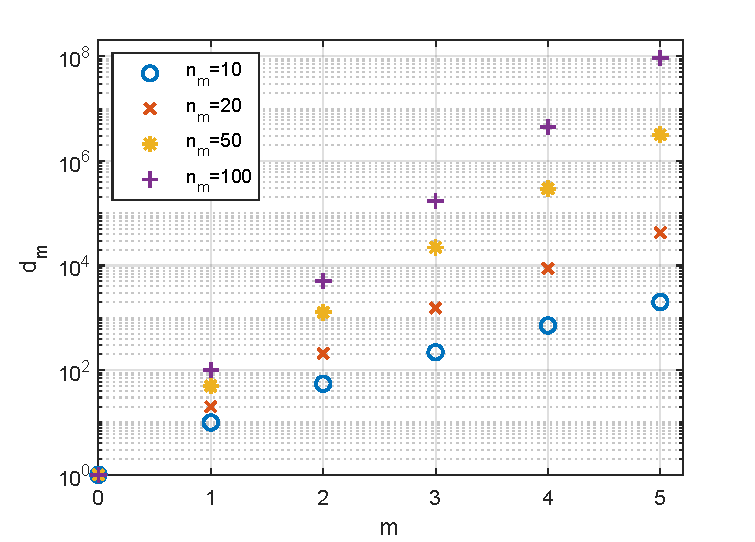
\includegraphics[width=0.65\textwidth]{Chapter3_VolterraSeries/ParameterGrowthB.pdf}
\caption{Number of unique kernel parameters for varying dimension and memory length}
\label{fig:ParameterGrowthCurse}
\end{figure}

The final consideration which must be made is stability. In the case of linear systems, bounded-input bounded-output (BIBO) stability can be defined easily using the impulse response representation. In particular for discrete-time models, a necessary and sufficient condition is that the impulse response be absolutely summable:
\begin{equation}
\sum_{\tau=0}^{\infty} |h(\tau)| < \infty.
\end{equation}
For Volterra series models, the situation is similar but not quite as straightforward. 
\begin{property}
For a causal Volterra kernel $h_m(\tau_1, \hdots, \tau_m)$, the kernel is BIBO stable if
\begin{equation}
\sum_{\tau_1=0}^{\infty} \hdots \sum_{\tau_m=0}^{\infty}|h_m(\tau_1, \hdots, \tau_m)| < \infty.
\end{equation}
\end{property}
The condition that the kernel be absolutely summable is sufficient to give BIBO stability, however it is no longer a necessary condition for $m>1$. Furthermore, a method for constructing stable kernels which violate this condition can be found in \cite{Schetzen1980}. While such special cases exist, in practice one would expect the kernels to decay to zero in all directions of increasing lag, implying that we have absolute summability.

Having established some important properties of the Volterra series and its associated kernels, the following assumption will hold true for the remainder of the thesis.
\begin{assum}
All nonlinear systems considered in this thesis can be represented by Volterra series models which contain causal, symmetric, and absolutely summable kernels.
\end{assum}

\section{Relationship to common block structures}
\label{sec:BlockStructureRelationship}

While block-oriented models are not the focus of this thesis, some of the more common block structures can be related to an equivalent Volterra series representation in an explicit sense. These relationships have been explored in e.g. \cite{Westwick2003} and \cite{Kibangou2010}, and will be used in the sequel to generate simulated Volterra systems with which to test the proposed algorithms. First, some assumptions are placed on the static nonlinear and linear dynamic blocks.

\begin{assum}
\label{assum:polynomialnonlin_Chap3}
In all block structures, the static nonlinear block can be represented by a polynomial nonlinearity\footnote{The polynomial assumption on $F(x(t))$ is not particularly restrictive, since any continuous function can be approximated arbitrarily well (in a least squares sense) over a finite interval by a polynomial of sufficiently high degree \cite{Timan1963}. For discontinuous functions, a similar pointwise convergence can be established as polynomial degree approaches infinity.},
$$F(x(t)) = \beta_0 + \beta_1 [x(t)] + \hdots + \beta_M [x(t)]^M.$$
\end{assum}

\begin{assum}
\label{assum:linearblock_Chap3}
In all block structures, the linear blocks are stable rational filters which can be represented by their corresponding impulse response, $g_i(\tau)$ for some integer subscript $i$.
\end{assum}

With these assumptions in place, three of the most well known block-oriented models are introduced, and their relationship to the Volterra series representation is defined.

\subsection{Wiener model}

The Wiener block structure consists of a single linear filter followed by a static nonlinear block to generate the output. A block diagram is provided in Figure \ref{fig:WienerBS}.

\begin{figure}[!h]
\centering
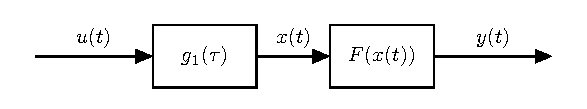
\includegraphics[scale=1]{Chapter3_VolterraSeries/WienerSystem.pdf}
\caption{Block structure for a Wiener model}
\label{fig:WienerBS}
\end{figure}

For the Wiener model, equivalent Volterra kernels are generated as follows,
\begin{align}
h_0 &= \beta_0, \nonumber \\
h_m(\tau_1,\hdots,\tau_m) &= \beta_m \cdot g_1(\tau_1) \cdot \hdots \cdot g_1(\tau_m).
\end{align}

\subsection{Hammerstein model}

The Hammerstein model contains the same two blocks as the Wiener model, but in the opposite order, i.e. a static nonlinear block followed by a linear filter. The structure is represented in Figure \ref{fig:HammersteinBS}.

\begin{figure}[!h]
\centering
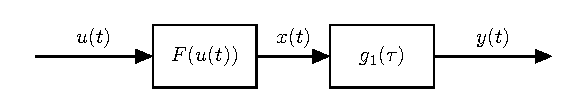
\includegraphics[scale=1]{Chapter3_VolterraSeries/HammersteinSystem.pdf}
\caption{Block structure for a Hammerstein model}
\label{fig:HammersteinBS}
\end{figure}

Hammerstein systems can also be represented using a series of Volterra kernels, i.e.
\begin{align}
h_0 &= \beta_0, \nonumber \\
h_m(\tau_1,\hdots,\tau_m) &= \begin{cases} \beta_m g_1(\tau_1) & \tau_1 = \hdots = \tau_m, \\ 0 & \textrm{otherwise}. \end{cases}
\end{align}
The kernels are seen to be nonzero only on their diagonal elements.

\subsection{Wiener-Hammerstein model}

The Wiener-Hammerstein model has the structure shown in Figure \ref{fig:WienerHammBS}, which is seen to be a combination of the previous two models. In such systems, the static nonlinear block is both preceded and followed by a linear filter. Clearly, Wiener-Hammerstein models are capable of describing a broader range of systems than Wiener and Hammerstein models, since the latter two are just special cases of the former.

\begin{figure}[!h]
\centering
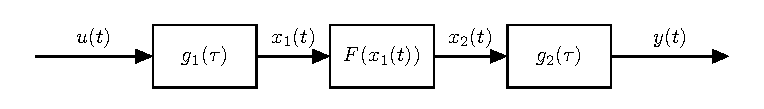
\includegraphics[scale=1]{Chapter3_VolterraSeries/WienerHammSystem.pdf}
\caption{Block structure for a Wiener-Hammerstein model}
\label{fig:WienerHammBS}
\end{figure}

The Volterra kernels corresponding to the Wiener-Hammerstein model are found via
\begin{align}
h_0 &= \beta_0, \nonumber \\
h_m(\tau_1,\hdots,\tau_m) &= \beta_m \sum\limits_{\tau=-\infty}^{\infty} g_2(\tau) \cdot g_1(\tau_1 - \tau) \cdot \hdots \cdot g_1(\tau_m - \tau).
\end{align}

\section{History of Volterra series identification}
\label{sec:VolterraID_History}

Despite the curse of dimensionality, the earliest results on Volterra series identification attempted to use classical methods from statistics involving input-output cross-correlations. Such methods were made more feasible by the development of the Wiener series \cite{Schetzen1974}, which is a variation of the Volterra series that is orthogonal (in discrete-time) for Gaussian white noise input. Estimation of the Wiener series could then be performed individually for each Wiener kernel by computing cross-correlations from experimental data \cite{Lee1965}.

Of course, the assumption of a Gaussian white noise input is too strict to be useful in many practical settings, and significant effort was put towards broadening the applicability of the cross-correlation approach. An extension for coloured (correlated) Gaussian inputs was proposed in \cite{Korenberg1990}, and extensions to other input distributions can be found in \cite{Ogura1972} and \cite{Segall1976}. Despite these efforts, estimation using cross-correlations was not a very efficient tool, requiring very large sample sizes for proper convergence, even in small, low-order problems \cite{Franz2006}.

Apart from using inputs with a known distribution, researchers specifically designed the identification input to maximize the accuracy of their chosen estimator. Some examples of these inputs include pseudorandom binary sequences (PRBS) in \cite{Sutter1987} and \cite{Reed1996}, and pseudorandom multilevel sequences (PRMLS) in \cite{Nowak1994}. These techniques are only applicable if the input used for identification can be precisely controlled, which is not always a realistic assumption.

More recently, the strategy of expanding Volterra series models in terms of a finite set of basis functions has come to the forefront. Such methods can provide a dramatic reduction in the number of parameters requiring estimation, providing the basis functions are chosen appropriately. The earliest examples of this approach appeared in \cite{Amorocho1971} for a hydrologic system, and \cite{Watanabe1975} for a physiological system, which then inspired further results in \cite{Ogura1985} and \cite{Marmarelis1993}. The popularity of the approach gained momentum following papers on the optimal Laguerre \cite{Campello2004} and Kautz \cite{Rosa2007} basis function expansions for Volterra models. As well as the classical sets of orthonormal functions, wavelets have also been explored as a basis due to their desirable properties of orthogonality and compact support \cite{Cheng2017}. Some notable examples can be found in \cite{Nikolaou2000}, \cite{Prazenica2004} and \cite{Prazenica2006}, however these methods are limited to kernels of order three and lower. 

The rapid increase of available computing power in recent decades has allowed more computationally intensive methods to enter the field of Volterra series estimation. A method based on particle swarm optimization was proposed in \cite{Chang2012}, while a relationship between the series and neural networks was discussed in \cite{Wray1994} and used to propose an identification scheme. Regularized linear regression was explored in \cite{Franz2006} using ridge regression. Finally, the Bayesian regularization approach \cite{Birpoutsoukis2017} of interest in this thesis is made possible via intensive global optimization techniques.

The discussion so far has only focussed on time domain estimation, since frequency domain kernels can be obtained indirectly from transformation of the time domain terms. Direct frequency domain estimation has its own history, however, which runs in parallel and follows the same trends as the time domain. Estimation of a system's GFRFs was originally considered for specific and strict experimental conditions. Methods in \cite{Bedrosian1971} required harmonic or Gaussian noise inputs, while \cite{Jones1989} required special harmonic inputs as well as readily available difference equations for the system. Many results employed specially designed periodic multisine inputs, such as \cite{Victor1980}, \cite{Boyd1983}, \cite{Chua1989} and \cite{Evans1996}. More recently, an interpolation method was provided in \cite{Nemeth2002} which exploits the (assumed) local smoothness of GFRFs, and another method has been proposed in \cite{Li2011} which directly uses harmonic time domain data for estimation.       

\section{Regularized Volterra series estimation}
\label{sec:RegVolterraTD}

Inspired by the success of Bayesian regularization techniques in linear impulse response identification \cite{Pillonetto2010}, an extension of the method to the Volterra series was first proposed in \cite{Birpoutsoukis2015}, and further improved in \cite{Birpoutsoukis2017} and \cite{Birpoutsoukis2017c}. The approach is conceptually similar, since each Volterra kernel is a multidimensional impulse response, however the extra dimensions add complexity when designing prior covariances for the kernels. While the properties of smoothness and decay are still integral to the process, they must now be imposed across the entire (hyper)surface of each kernel.

First, assumptions must be placed on the model structure for the system.
\begin{assum}
\label{ass:ReLSmodelstructure}
The system can be represented by a Volterra series model with known deterministic input and white Gaussian measurement noise, $e(t) \sim \mathcal{N}(0,\sigma^2)$, added directly at the output. The measured output, $y$, is then given by 
\begin{equation}
\label{eq:ReLS_VolterraModelStructure}
y(t) = y^0(t) + e(t),
\end{equation} 
where $y^0(t)$ is the noise-free Volterra series output from (\ref{eq:VolterraTimeDomainOutput}). 
\end{assum}

From the assumed model structure, a linear regression formulation of the problem can now be considered, i.e.
\begin{equation}
\label{eq:VolterraRegressionForm}
Y = \Phi^T \theta + E,
\end{equation}
where $Y, E \in \mathbb{R}^{N-n+1}$ are the vectors of output measurements and measurement noise respectively, and $\theta = [h_0, {h_1^\mathcal{V}}^T, {h_2^\mathcal{V}}^T, \hdots, {h_M^\mathcal{V}}^T]^T \in \mathbb{R}^D$ is the parameter vector containing all unique coefficients for each Volterra kernel. For the multi-dimensional kernels, $h_m^\mathcal{V} \in \mathbb{R}^{d_m}$ refers to a vector containing the unique kernel coefficients in $h_m(\tau_1,\hdots, \tau_m)$. The regressor matrix, $\Phi \in \mathbb{R}^{D \times (N-n+1)}$, should be constructed based on the vectorization scheme used in $\theta$, and must take into account the assumed symmetry of kernels in the series. While each kernel's coefficients are free to be ordered in an arbitrary fashion, a structured approach to vectorization is detailed in \cite{Birpoutsoukis2017} for the second order case. A small illustrative example will be given here.   

Consider a 2\textsuperscript{nd} order Volterra series model, with memory lengths ${n_1=n_2=n=3}$ for the kernels. The parameters requiring estimation in this model are depicted in Figure \ref{fig:VolterraRegressionExample}, where black circles indicate unique coefficients to be estimated, and red circles indicate non-unique coefficients which will be estimated. The gray dashed circles give the non-unique coefficients which will not be estimated, but rather inferred using their symmetrical red counterparts. The resulting regression structure is then given by,
\begin{figure}[t]
\centering
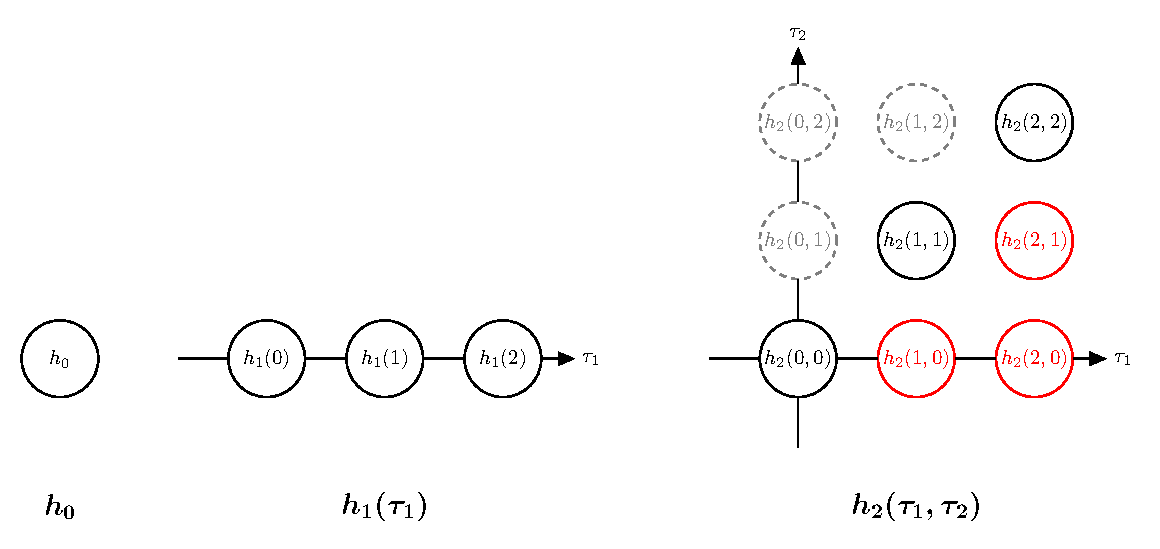
\includegraphics[width = 0.95\textwidth]{Chapter3_VolterraSeries/VolterraSeriesRegressionExample.pdf}
\caption{Estimation parameters in a 2\textsuperscript{nd} order Volterra series with memory length 3}
\label{fig:VolterraRegressionExample}
\end{figure}
\begin{equation*}
\begin{bmatrix} y(2) \\ y(3) \\ \vdots \\ y(N-1) \end{bmatrix} = 
\begin{bmatrix} 1 & 1 & \hdots & 1 \\ u(2) & u(3) & \hdots & u(N-1) \\ u(1) & u(2) & \hdots & u(N-2) \\ u(0) & u(1) & \hdots & u(N-3) \\
u(2) \cdot u(2) & u(3) \cdot u(3) & \hdots & u(N-1) \cdot u(N-1) \\ \textcolor{red}{2} u(1) \cdot u(2) & \textcolor{red}{2} u(2) \cdot u(3) & \hdots & \textcolor{red}{2} u(N-2) \cdot u(N-1) \\
\textcolor{red}{2} u(0) \cdot u(2) & \textcolor{red}{2} u(1) \cdot u(3) & \hdots & \textcolor{red}{2} u(N-3) \cdot u(N-1) \\ u(1) \cdot u(1) & u(2) \cdot u(2) & \hdots & u(N-2) \cdot u(N-2) \\
\textcolor{red}{2} u(0) \cdot u(1) & \textcolor{red}{2} u(1) \cdot u(2) & \hdots & \textcolor{red}{2} u(N-3) \cdot u(N-2) \\ u(0) \cdot u(0) & u(1) \cdot u(1) & \hdots & u(N-3) \cdot u(N-3) \end{bmatrix}^T  
\begin{bmatrix} h_0 \\ h_1(0) \\ h_1(1) \\ h_1(2) \\ h_2(0,0) \\ \textcolor{red}{h_2(1,0)} \\ \textcolor{red}{h_2(2,0)} \\ h_2(1,1) \\ \textcolor{red}{h_2(2,1)} \\ h_2(2,2) \end{bmatrix} + E.
\end{equation*}
Note the non-unique coefficients (highlighted in red) in the parameter vector, which have their regressor entries multiplied by 2 since they represent the contribution of 2 symmetric coefficients in the second order kernel.

Given the model structure assumption in (\ref{eq:ReLS_VolterraModelStructure}), it was shown in Chapter \ref{chap:2} that both the least squares and maximum likelihood estimate of $\theta$ will be given by the analytic solution,
\begin{equation}
\label{eq:LSestimator_VolterraSeries}
\hat{\theta}_{LS} = (\Phi \Phi^T)^{-1} \Phi Y.
\end{equation}

Since the least squares estimation problem is likely to be ill-conditioned or even underdetermined for a Volterra model with large numbers of parameters, we regularize the estimate with a Bayesian-tuned quadratic penalty. The Bayesian method proposed in \cite{Birpoutsoukis2017} treats each Volterra kernel in the model as an independent Gaussian process with a separate prior covariance, outlined in the following assumption.
\begin{assum}[Gaussian priors]
Every vector of kernel coefficients, $h_m^\mathcal{V}$, is a zero mean Gaussian process: 
\begin{equation}
h_m^\mathcal{V} \sim \mathcal{N}(0,P_m) \; \; \; m = 1, \hdots, M.
\end{equation}
Furthermore, all pairs of coefficient vectors, $h_i^\mathcal{V}$ and $h_j^\mathcal{V}$, are independent for $i \neq j$.

The constant offset is also Gaussian, i.e. $h_0 \sim \mathcal{N}(0,P_0)$, and is independent of all other kernels.
\end{assum}

This Bayesian assumption frames the total parameter vector as a Gaussian process, i.e. $\theta \sim \mathcal{N}(0,P)$, where $P$ is the total prior covariance constructed as a block diagonal matrix,
\begin{equation}
\label{KernelPenalty}
P = \begin{bmatrix}
       P_0 & & &  \multirow{2}{*}{\huge 0} \\
       & P_1 & & \\
      \multirow{2}{*}{\huge 0} & & \ddots & \\
       &  & & P_M
     \end{bmatrix},
\end{equation}
with $P_m \in \mathbb{R}^{d_m \times d_m}$ being the prior covariance for the $m$\textsuperscript{th} Volterra kernel. 

Individually, the prior covariance matrices should be designed to impose smoothness and exponential decay on their multi-dimensional kernels, as in the FIR case. For $P_1$, the TC structure in (\ref{eq:TCstructure}) or DC structure in (\ref{eq:DCstructure}) can be directly applied, since $h_1$ is effectively an impulse response. For kernel dimensions greater than one, the TC or DC structure must be incorporated into a more complex covariance matrix in order to impose smoothness and stability along the entire (hyper)surface. The approach suggested in \cite{Birpoutsoukis2017} is to consider $m$ perpendicular regularizing directions for the kernel $h_m$, where the vector $(1,\hdots,1)$ is always included as one of the directions. As an example, the regularizing directions for a second order kernel are shown in Figure \ref{fig:SecondOrderRegDir}. A rotated coordinate system can be formed from the set of regularizing vectors, which we will denote $(v_m^1, \hdots, v_m^m)$.  

\begin{figure}[h]
\centering
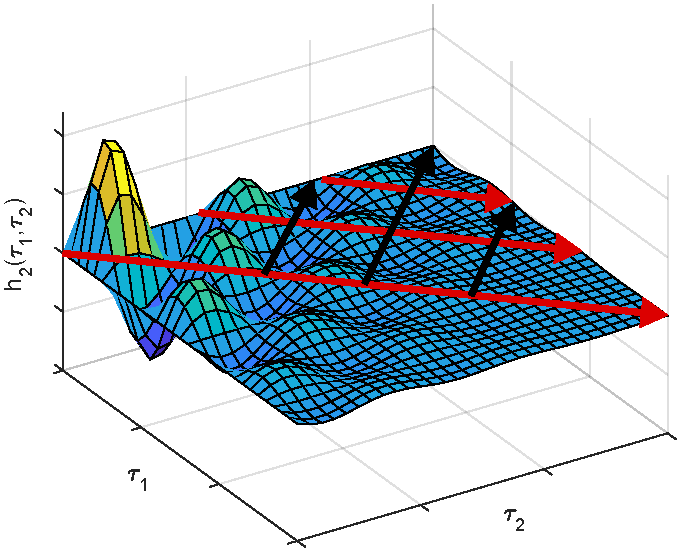
\includegraphics[width = 0.6\textwidth]{Chapter3_VolterraSeries/RegDirections3.pdf}
\caption{The two perpendicular regularizing directions, (1,1) (red) and (-1,1) (black), for a second order Volterra kernel}
\label{fig:SecondOrderRegDir}
\end{figure}

\begin{rem}
A suitable set of orthogonal regularizing directions for the $m$\textsuperscript{th} nonlinear order can be obtained via the following standard form (for $m \geq 3$):
\begin{equation}
\begin{split}
v_m^1 &= (1,1,\hdots,1), \\
v_m^2 &= (-1,\hdots,-1,m-1) \\
v_m^3 &= (-1,\hdots,-1,m-2,0) \\
&\hdots \\
v_m^m &= (-1,1,0,\hdots,0)
\end{split}
\end{equation}
\end{rem}

The rotated coordinate system is used to apply the chosen covariance structure along each regularizing direction, forming a set of $m$ partial covariance matrices. For the regularizing direction $v_m^j$, the corresponding partial covariance matrices for the TC and DC structures are,
\begin{align}
\label{TCext}
&\textbf{TC structure:} \hfill &P_m^j(x,y) = (\lambda_m^j)^{max(x',y')}, \\
&\textbf{DC structure:} \hfill &P_m^j(x,y) = (\lambda_m^j)^{(x' + y')/2} (\rho_m^j)^{|x'-y'|},
\label{DCext}
\end{align}
where $x'$ is the coordinate of $h^{\mathcal{V}}_{m}(x)$ on the $v_m^j$ axis. If $h^{\mathcal{V}}_{m}(x)$ is associated with lag values $\bm{\tau} = (\tau_1, \hdots, \tau_m)$, then $x' = \langle \bm{\tau} , v_m^j \rangle$. An Hadamard product of the partial covariances is required to produce the total prior covariance for the kernel, i.e.
\begin{equation}
\label{FinalPenalty}
P_m = c_m \cdot P_m^1 \circ \hdots \circ P_m^m, \; \; \; \; m = 1, \hdots, M.
\end{equation}
where $c_m$ is a normalization hyperparameter. The covariance for $h_0$ is simply given by 
\begin{equation}
P_0 = c_0.
\end{equation}

There are clearly a large number of hyperparameters which require empirical tuning to form our regularization penalty, $P$. More specifically, there are $m+1$ hyperparameters per kernel when using a TC structure, which include the normalization constant, $c_m$, and $m$ decay constants, $\lambda_m^j$. Using the DC structure increases this to $2m+1$ hyperparameters per kernel, by including the $\rho_m^j$ set. In either case, the suggested method for hyperparameter tuning in \cite{Birpoutsoukis2017} is to use the standard marginal likelihood maximization of (\ref{eq:MarginalLikelihood_opt}). While the optimization is still applicable in the Volterra series case, the large dimension of the search space and non-convexity of the problem can yield prohibitively long computation times, with a high risk of settling in sub-optimal local minima. These complications motivate the research in Chapter \ref{chap:4} of this thesis.

Following the hyperparameter tuning (which may also include noise variance $\sigma^2$), $P$ can be constructed, and the regularized estimate of $\theta$ may be obtained analytically from (\ref{eq:MLE_BayesianRegularization}).

As an illustration of the profound benefit of Bayesian regularization in Volterra series estimation, parameter estimates have been obtained for a simple 2\textsuperscript{nd} order example system, whose true kernels are shown in Figure \ref{fig:ExampleLSvsReLS_TrueKernels}. Estimates of these kernels were obtained using 
\begin{enumerate}
\item A simple least squares estimator (\ref{eq:LSestimator_VolterraSeries})
\item A regularized estimate (\ref{eq:MLE_BayesianRegularization}) with empirically tuned TC structure for $P$ via (\ref{KernelPenalty}), (\ref{TCext}) and (\ref{eq:MarginalLikelihood_opt})
\end{enumerate}

\begin{figure}[h]
\centering
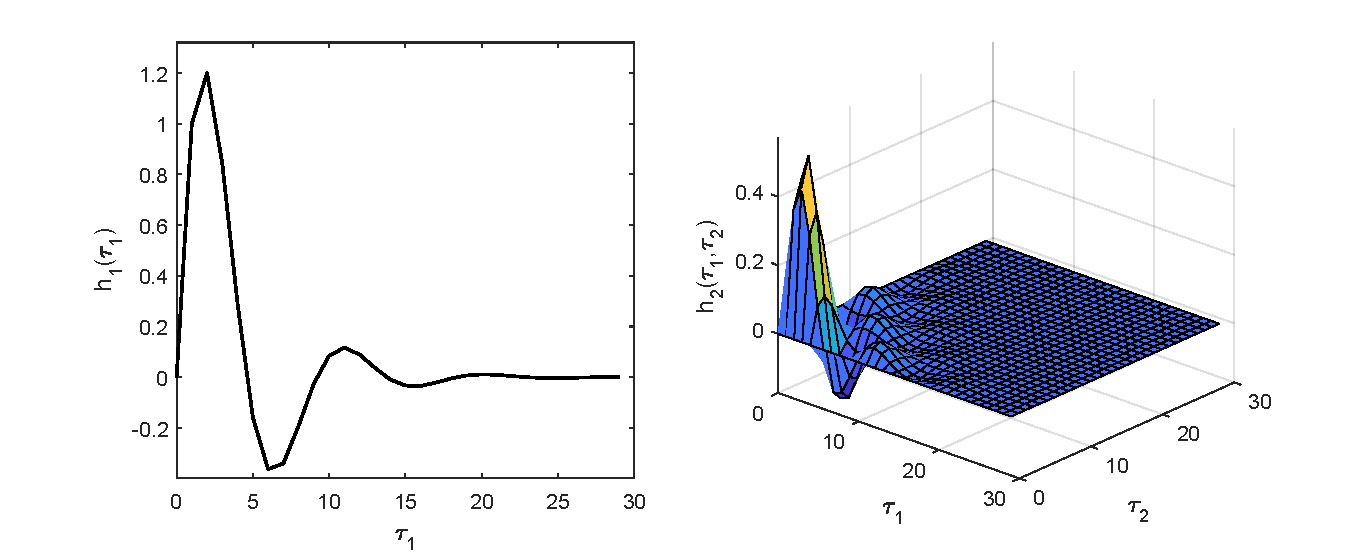
\includegraphics[width = 1\textwidth]{Chapter3_VolterraSeries/LSvsReLS_truekernels.pdf}
\caption{True Volterra kernels for the comparative simulation example}
\label{fig:ExampleLSvsReLS_TrueKernels}
\end{figure}

The first set of estimates, shown in Figure \ref{fig:ExampleLSvsReLS_VolterraSeries2_whitenoise}, were obtained from a simulation of the system in Figure \ref{fig:ExampleLSvsReLS_TrueKernels} for a dataset with length $N=1000$, noise variance $\sigma^2 = 1$, and a white Gaussian noise input. In this case, the input signal is sufficiently exciting, however the least squares estimate still suffers from high covariance due to the large number of parameters being estimated. The regularized estimator, however, produces smooth, accurate estimates of the Volterra kernels due to the construction of prior covariances which impose the desired behaviour. 

The second set of estimates, shown in Figure \ref{fig:ExampleLSvsReLS_VolterraSeries2_filterednoise}, were obtained using the same specifications, except that the input is now \emph{filtered} Gaussian noise. In this case the input does not have energy in the full frequency band (i.e. it is not sufficiently exciting), hence the least squares estimator is ill-conditioned and the resulting estimate is unusable. The regularized estimate, on the other hand, is relatively unaffected by the change. 

\vspace{10mm}

\begin{figure}[!hp]
\centering
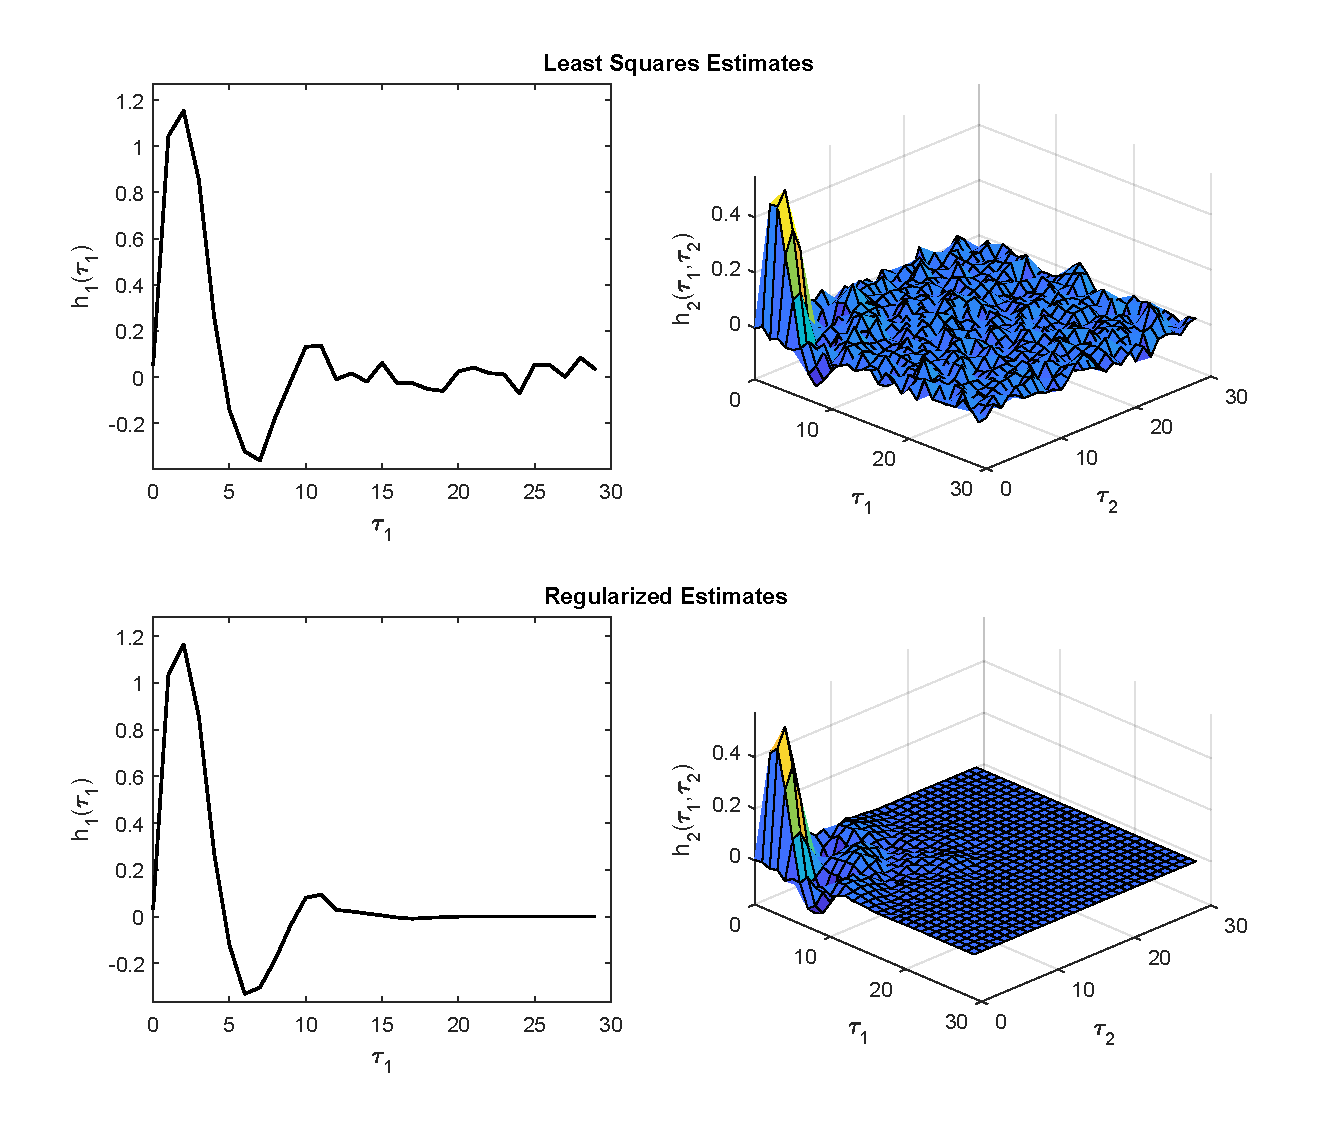
\includegraphics[width = 1.1\textwidth]{Chapter3_VolterraSeries/LSvsReLS_whiteinput.pdf}
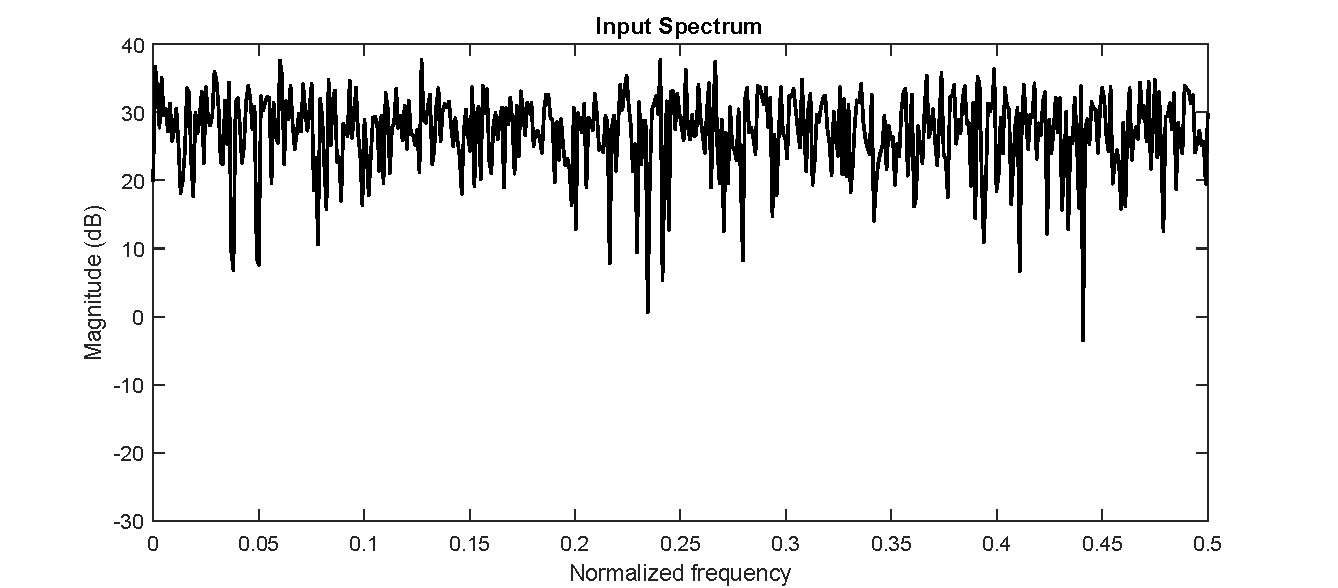
\includegraphics[width = 1.1\textwidth]{Chapter3_VolterraSeries/white_spectrum.pdf}
\caption{Least squares (top) and regularized (middle) kernel estimates for a white Gaussian input (bottom)}
\label{fig:ExampleLSvsReLS_VolterraSeries2_whitenoise}
\end{figure}

\begin{figure}[!hp]
\centering
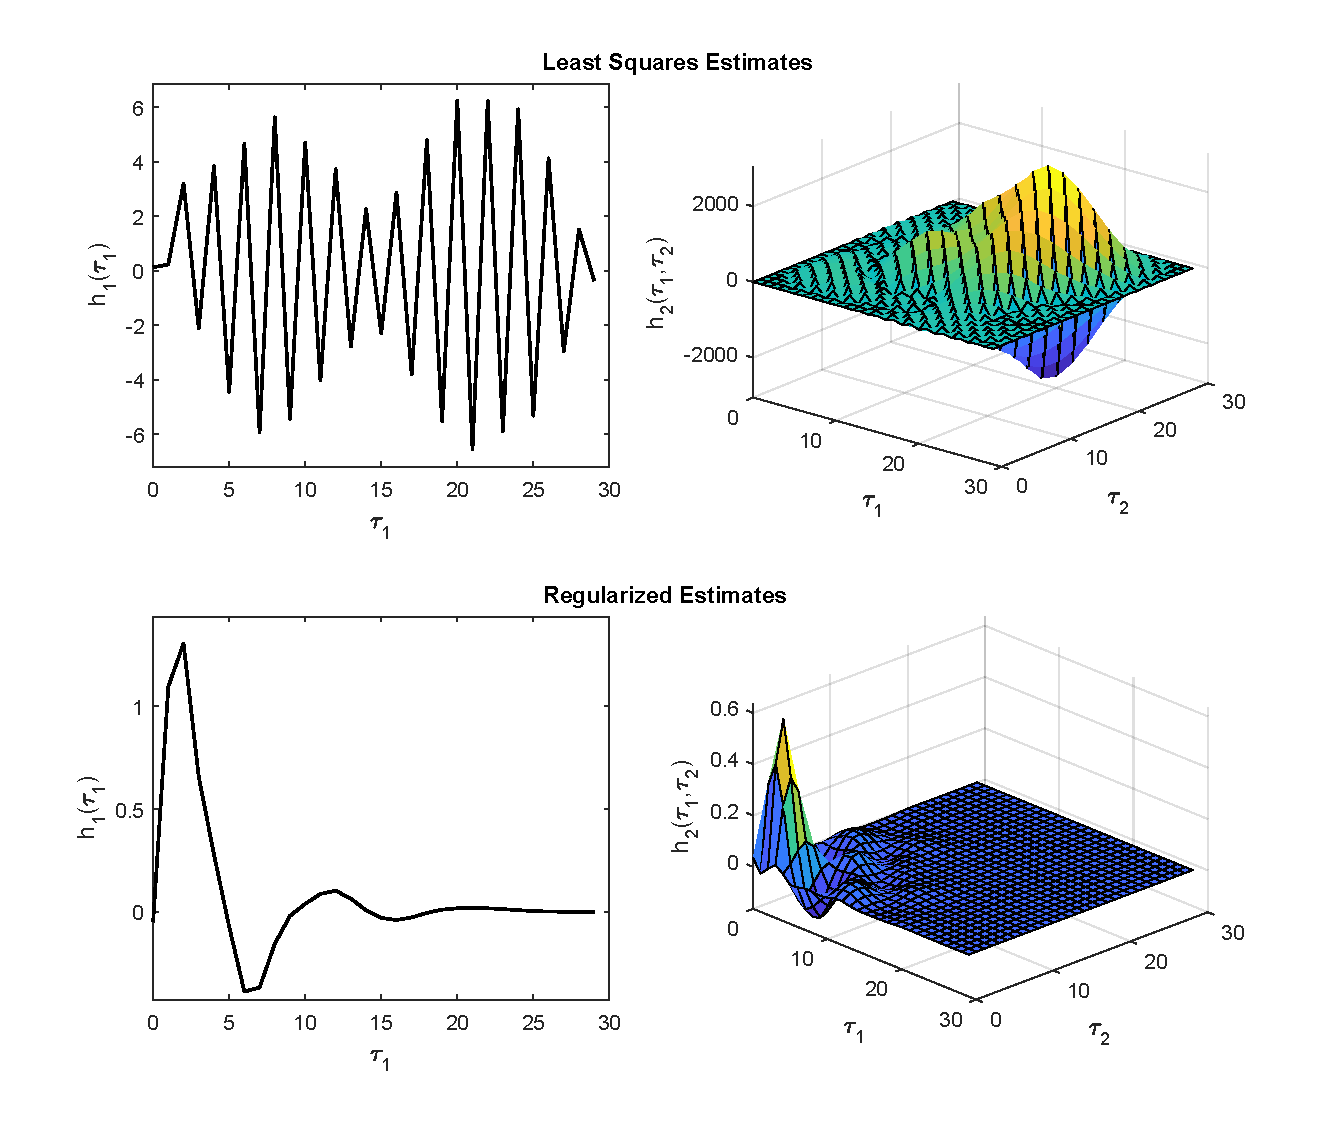
\includegraphics[width = 1.1\textwidth]{Chapter3_VolterraSeries/LSvsReLS_butterworthinput.pdf}
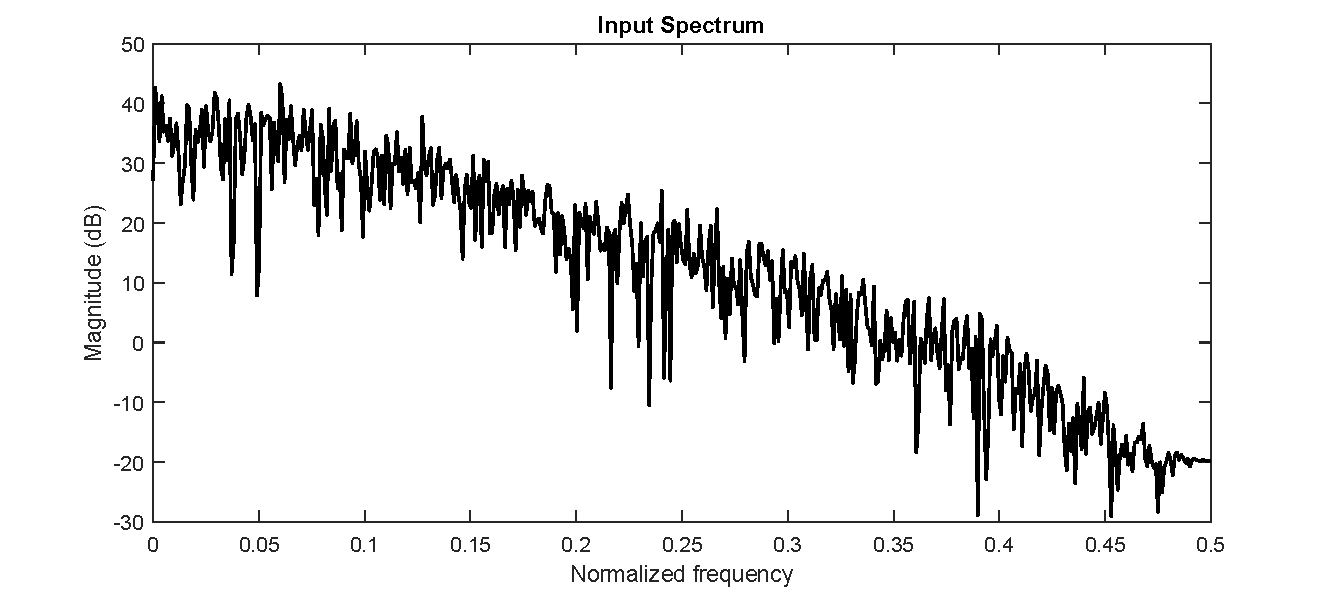
\includegraphics[width = 1.1\textwidth]{Chapter3_VolterraSeries/butterworth_spectrum.pdf}
\caption{Least squares (top) and regularized (middle) kernel estimates for a filtered Gaussian input (bottom)}
\label{fig:ExampleLSvsReLS_VolterraSeries2_filterednoise}
\end{figure}
 
\section{Summary}
 
The Volterra series model for nonlinear dynamical systems was introduced in this chapter, with discrete-time representations defined in both the time and frequency domain. Assumptions of causality, stability and symmetry were established for each Volterra kernel in the series, and the parameter growth issue (i.e. the curse of dimensionality) was discussed. Previous results on the identification of Volterra series models were summarized, and particular attention was paid to the Bayesian regularization method proposed recently in the literature. The regularized approach was developed for time domain identification, and will serve as a foundation for the extensions proposed in Part \ref{part:TD} of this thesis, as well as inspiration for many of the frequency domain contributions in Part \ref{part:FD}.

%--------------------------------------------------------------------------------------------------------------------------------------------------
\cleardoublepage
\part{Time Domain Identification}
\label{part:TD}
%--------------------------------------------------------------------------------------------------------------------------------------------------

\cleardoublepage
\chapter{EM-Based Hyperparameter Optimization for Regularized Volterra Series Estimation}
\label{chap:4}
\emph{The Bayesian regularization method for estimating Volterra series models suffers from poor computation time scaling with respect to the series order. The scaling problem arises in the marginal likelihood maximization used for hyperparameter tuning, where the dimension of the search space grows quadratically with series order. A further problem also arises in the fact that the cost function can have a large number of local minima. In this chapter, the hyperparameter optimization is reformulated using an expectation-maximization (EM) approach, which reduces the single large optimization problem to a set of smaller problems in an iterative scheme. The maximum search space dimension of these smaller problems increases linearly with the order of the Volterra series, thereby improving the computation time scaling of regularized estimation. Both the traditional marginal likelihood and proposed EM approach are applied to numerical examples to confirm the superior computation time scaling of the EM method.}
\newpage
\section{Introduction}

The Volterra series provides a linear-in-the-parameters representation for a broad class of nonlinear systems, however we have seen in Chapter \ref{sec:RegVolterraTD} that the estimation of its associated Volterra kernels is ill-suited to a standard least squares framework. This is because the nonparametric nature of the model implies a requirement for large numbers of parameters, which in turn produces large variances in least squares estimates obtained from a finite and noisy data record. 

In order to reduce the variance of kernel estimates, a regularized least squares approach was developed in \cite{Birpoutsoukis2017} and \cite{Birpoutsoukis2017c}. As discussed in Chapter \ref{chap:3}, the method uses Bayesian techniques to impose smoothness and decay along the (hyper)surfaces of each Volterra kernel, which is a nonlinear extension of Bayesian impulse response identification as introduced in \cite{Pillonetto2010}. The regularized estimation employs a set of tunable hyperparameters to describe the smoothness and decay rates of each kernel, where traditionally such hyperparameters have been optimized through a maximization of the associated marginal likelihood expression, which is typically non-convex \cite{Chen2013}. The dimension of the search space for this optimization increases quadratically with the order of the Volterra series model, since decay hyperparameters are required for each dimension of each kernel.

When compared to standard least squares and other more traditional estimation methods, the main disadvantages of the regularization approach in \cite{Birpoutsoukis2017} are:
\begin{itemize} 
\item Increased computational cost,
\item Poor computation time scaling with the maximum series order, $M$,
\item Risk of converging to a local minimum in the hyperparameter optimization 
\end{itemize}
These disadvantages are directly acknowledged in the concluding remarks of \cite{Birpoutsoukis2017}, which states:
\begin{quote}
``Several issues should be addressed in the future, such as efficient ways to optimize the hyperparameters of the regularization matrix in order to reduce the risk of resulting in a local minimum of the marginal likelihood.''
\end{quote} 

To address the issues of computation time scaling and non-convexity, an alternative hyperparameter tuning method is developed in this chapter. The new method is proposed within the expectation-maximization (EM) framework \cite{Dempster1977}, and is inspired by results from \cite{Bottegal2015} and \cite{Bottegal2016} which deal with linear system identification. When applied to Volterra series estimation, the approach will be shown to trade the single large optimization problem in \cite{Birpoutsoukis2017} for a set of smaller problems in an iterative scheme, where the maximum dimension of the search space increases linearly with the series order. 

Numerical examples in Section \ref{sec:NumEx_EM} confirm that computation times for the EM-based formulation do not increase as rapidly with series order, while still converging to the same hyperparameters as the marginal likelihood optimization traditionally used in these problems.

\section{The expectation-maximization algorithm}

`Expectation-maximization' refers to a family of computation methods designed to find maximum likelihood estimates in cases where there are latent (unobserved) variables \cite{McLachlan2007}. These latent variables may represent real unobserved data, or (as is the case in this thesis) they can be `nuisance parameters' resulting from the reformulation of an estimation problem. 

In the general case, consider a data vector, $X$, which is a concatenation of two subvectors:
\begin{equation}
X = \begin{bmatrix} Y \\ Z \end{bmatrix},
\end{equation}
where $Y$ is the vector of \emph{observed} data, while $Z$ represents the \emph{unobserved} variables. Assume further that $X$ is drawn from some distribution, $p_c(Y,Z ; \eta)$, which is described by the unknown parameters, $\eta$. Under these conditions, the maximum likelihood estimation of $\eta$ is the problem of interest, i.e.
\begin{equation}
\hat{\eta} = \text{arg } \underset{\eta}{\text{max }} L_c(Y,Z ; \eta),
\label{eq:EM_jointlikelihoodopt}
\end{equation}
where $L_c(Y,Z ; \eta) = \log p_c(Y, Z; \eta)$ is the log likelihood function for the complete data vector, $X$. However since the $Z$ portion of data is not observed, (\ref{eq:EM_jointlikelihoodopt}) cannot be used directly.

One possible solution is to produce a marginal likelihood function by integrating out the latent variables from our distribution, yielding a marginal likelihood maximization (MLM) problem:
\begin{align}
\hat{\eta} &= \text{arg } \underset{\eta}{\text{max }} \log \int_Z p_c(Y,Z; \eta) \text{d}Z \\
&= \text{arg } \underset{\eta}{\text{max }} \log p(Y; \eta).
\label{eq:EM_marginallikelihoodopt}
\end{align}
Indeed, this is the typical pathway for regularized estimation problems employing empirical Bayes techniques \cite{Pillonetto2010}, \cite{Birpoutsoukis2017}, \cite{Lataire2016}.

There are many circumstances where a marginal likelihood approach becomes undesirable. For example, the marginalization process may be impossible or computationally intractable to perform, or it may be that the resultant optimization problem (\ref{eq:EM_marginallikelihoodopt}) is extremely difficult to solve. The latter problem is relevant to regularized Volterra series estimation, where the marginal likelihood approach implies searching through a high-dimensional non-convex function. In these situations, EM methods provide an alternate pathway which often resolves the issues associated with marginalization.

In essence, the EM approach moves back to the complete data problem, (\ref{eq:EM_jointlikelihoodopt}), but replaces the unobserved data, $Z$, with its expected value given $Y$ and some guess of $\eta$. While there is no reason to believe this guess is accurate, the procedure can be repeated iteratively with nice convergence properties for $\eta$. 

Conceptually, the iterative procedure for the EM method consists of two steps. The first is the \emph{expectation} step, where the complete data likelihood function is approximated using parameters, $\hat{\eta}^{(k)}$, from the previous iteration, i.e.
\begin{equation}
\label{estep}
Q(\eta,\hat{\eta}^{(k)}) = \textbf{E}\{  L_c(Y,Z;\eta) \},
\end{equation}
where $Q$ is the likelihood approximation, and the expectation is taken with respect to the posterior distribution $p(Z|Y; \hat{\eta}^{(k)})$.

The second step consists of a \emph{maximization}, where the parameters are updated by maximizing the function (\ref{estep}) calculated in the first step. The new hyperparameters are thus given by,
\begin{equation}
\hat{\eta}^{(k+1)} = \text{arg } \underset{\eta}{\text{max }} Q(\eta,\hat{\eta}^{(k)}).
\end{equation}

The chain of successive parameter estimates, $\hat{\eta}^{(k)}$, is called an \emph{EM sequence}, and there are some useful properties of this sequence which can be exploited. Noting first that $Q(\eta,\hat{\eta}^{(k)})$ is a lower bound on the marginal likelihood, $\log p(Y; \eta)$, it can be shown that each new iteration of the EM sequence corresponds to a higher point in the marginal likelihood function. If we impose the reasonable assumption that the marginal likelihood is itself upper bounded, then it is straightforward to show that the EM sequence will converge to a stationary point of $p(Y; \eta)$ \cite{Wu1983}. While some artificial examples have been constructed in the literature which converge to saddle points or local minima \cite{McLachlan2007}, a local maximum is almost guaranteed in practice. Thus, the EM method provides an alternate route to MLM without the need for explicit marginalization.

There is another property of the EM method which is not supported by formal results, but has been noted anecdotally. In comparison to standard MLM, the equivalent EM approach is often found to be more robust to poor initialization, and therefore less likely to settle in a sub-optimal local maximum. Such behaviour is particularly important in the Volterra series context, where MLM can involve many local maxima in the high-dimensional search space \cite{Birpoutsoukis2017}.

\section{Hyperparameter optimization using EM}

For the Bayesian estimation problem outlined in Chapter \ref{sec:RegVolterraTD}, the parameter vector, $\theta$, is framed as a random variable which is jointly distributed with the output data, $Y$. The problem of hyperparameter optimization can thus be framed as likelihood maximization with latent variables. The original parameter vector, $\theta$, becomes the unobserved data, and we require an estimate of all hyperparameters $\eta$ describing the joint distribution, i.e. 
\begin{equation}
\hat{\eta} = \text{arg } \underset{\eta}{\text{max }} L_c(Y,\theta;\eta),
\end{equation}
where $ L_c(Y,\theta;\eta)$ is the joint log likelihood of $Y$ and $\theta$.

This interpretation has already led to the MLM approach defined in (\ref{eq:MarginalLikelihood_opt}), both for the linear FIR and Volterra series cases. In this section, the EM solution will be derived for hyperparameter tuning in Volterra kernels with Gaussian priors. Relevant modeling assumptions will be (re)stated below for convenience.

\begin{assum}
The data generating model is a Volterra system with white Gaussian additive noise (\ref{eq:ReLS_VolterraModelStructure}), and uses the vectorized regression structure given in (\ref{eq:VolterraRegressionForm}), i.e.
\begin{equation}
\label{eq:VolterraRegressionForm_Chap4}
Y = \Phi^T \theta + E,
\end{equation}
with $\theta = [h_0, {h_1^\mathcal{V}}^T, {h_2^\mathcal{V}}^T, \hdots, {h_M^\mathcal{V}}^T]^T$.
\label{ass:ModelStructure_Chap4}
\end{assum}

\begin{assum}
The parameter vector is a Gaussian random variable, $\theta \sim \mathcal{N}(0,P)$, with block diagonal prior covariance (\ref{KernelPenalty}). Individual kernel covariances are defined using the TC structure, via (\ref{TCext}) and (\ref{FinalPenalty}).
\label{ass:GaussianTheta_Chap4}
\end{assum}

While the derivation is performed here for the TC covariance structure, the DC structure and others can be derived in an almost identical fashion.

\subsection{The expectation step}

Under assumptions \ref{ass:ModelStructure_Chap4} and \ref{ass:GaussianTheta_Chap4}, the lower bound function $Q(\eta,\hat{\eta}^{(k)})$ in (\ref{estep}) can be constructed analytically from the normal distributions of $Y$ and $\theta$. First, the function is separated into two components,
\begin{equation}
\label{Qsplit}
Q(\eta,\hat{\eta}^{(k)}) = \textbf{E}\{  \log p(Y|\theta; \eta) \} + \textbf{E}\{ \log p(\theta; \eta) \}.
\end{equation}
It can be seen from (\ref{eq:VolterraRegressionForm_Chap4}) that $Y|\theta;\eta \sim \mathcal{N}(\Phi^T \theta,\sigma^2I)$, hence,
\begin{align}
\textbf{E}\{  \log p(Y|\theta; \eta) \} &= \textbf{E} \{ a_1 - \frac{N}{2} \log \sigma^2 - \frac{1}{2 \sigma^2}(Y^T Y - 2 Y^T \Phi^T \theta + \theta^T \Phi \Phi^T \theta) \} \nonumber \\
&= a_1 - \frac{N}{2} \log \sigma^2 \label{qnoise} - \frac{1}{2 \sigma^2}\big(Y^T Y - 2 Y^T \Phi^T \textbf{E}\{\theta\} + \text{Tr}[\Phi \Phi^T \textbf{E}\{ \theta \theta^T \}]\big),
\end{align}
where $a_1$ is a real number, and $\sigma^2 \in \eta$ is the only hyperparameter present in the expression. The remaining expected values in (\ref{qnoise}) are taken with respect to $p(\theta|Y; \hat{\eta}^{(k)})$, with analytic expressions obtained via the joint distribution of $\theta$ and $Y$,
\begin{equation}
\begin{bmatrix}
\theta \\ 
Y
\end{bmatrix} \sim \mathcal{N} \Bigg(
\begin{bmatrix}
0\\ 
0
\end{bmatrix},
\begin{bmatrix}
P & P \Phi\\ 
\Phi^T P & \Phi^T P \Phi + \sigma^2 I 
\end{bmatrix} \Bigg).
\end{equation}
Using the standard expressions for Gaussian conditional distributions, and applying the matrix inversion lemma, we can arrive at numerically robust expressions for the desired expected values, 
\begin{align}
&\textbf{E} \{ \theta \} = \textbf{E} \{ \theta | Y \} = P(\hat{\eta}^{(k)}) [\Phi \Phi^T P(\hat{\eta}^{(k)}) + [\hat{\sigma}^2]^{(k)} I]^{-1} \Phi Y, \\
&\textbf{Cov} \{ \theta| Y \} = [\hat{\sigma}^2]^{(k)} P(\hat{\eta}^{(k)}) [\Phi \Phi^T P(\hat{\eta}^{(k)}) + [\hat{\sigma}^2]^{(k)} I]^{-1}, \\
&\textbf{E} \{ \theta \theta^T\} = \textbf{Cov} \{ \theta| Y \} + \textbf{E} \{ \theta | Y \} \cdot \textbf{E} \{ \theta | Y \}^T,
\label{expect3}
\end{align}
where $P$ and $\sigma^2$ are constructed from the hyperparameters of the previous iteration, $\hat{\eta}^{(k)}$.

Returning to (\ref{Qsplit}), $\textbf{E}\{ \log p(\theta; \eta) \}$ can also be computed, given that $\theta$ is normally distributed by assumption in the Bayesian setting. The term can thus be written as,
\begin{align}
\textbf{E}\{ \log p(\theta; \eta) \} &= \textbf{E} \{ a_2 - \frac{1}{2} \text{log det} P(\eta) - \frac{1}{2} \theta^T P^{-1}(\eta) \theta \} \nonumber \\
&= a_2 - \frac{1}{2} \text{log det} P(\eta) - \frac{1}{2} \text{Tr}[ P^{-1}(\eta) \textbf{E}\{ \theta  \theta^T \}], 
\label{qP}
\end{align}
where $\textbf{E}\{ \theta  \theta^T \}$ can be evaluated using (\ref{expect3}), and $a_2$ is a real number independent of $\eta$. 

The block diagonal structure of $P$, given in (\ref{KernelPenalty}), can now be exploited to split (\ref{qP}) into smaller components.  As discussed earlier, we will consider TC-based prior covariances, however similar steps can be applied to any block diagonal structure. In order to partition the hyperparameters further, we require some new notation.

\begin{notation}
\label{not:decayparams}
The vector of decay hyperparameters for kernel $h_m$ is denoted
\begin{equation}
\bar{\eta}_m = [ \lambda_m^1, \hdots, \lambda_m^m] \; \; \; \; m = 1, \hdots, M.
\end{equation}
\end{notation}

\begin{notation}
\label{not:decomposedprior}
The kernel prior covariance $P_m$ can be expressed as
\begin{equation}
P_m = c_m \cdot \bar{P}_m(\bar{\eta}_m) \; \; \; \; m = 1, \hdots, M.
\end{equation}
For the 0\textsuperscript{th} order kernel, $h_0$, we have $\bar{P}_0 = 1$
\end{notation}

\begin{notation}
\label{not:Wmatrix}
The expected value, $\textbf{E} \{ \theta \theta^T\}$, is a matrix which can be decomposed as
\begin{equation}
\textbf{E} \{ \theta \theta^T\} = \begin{bmatrix}
       W_0 & & &  \multirow{2}{*}{\huge *} \\
       & W_1 & & \\
      \multirow{2}{*}{\huge *} & & \ddots & \\
       &  & & W_M
     \end{bmatrix},
\end{equation}
where $W_{m} \in \mathbb{R}^{d_m \times d_m}$ is a square matrix with the same dimension as $P_m$, and $*$ represents arbitrary off diagonal components.
\end{notation}

The two terms in (\ref{qP}) involving $P(\eta)$ can now be expressed in terms of summations over each nonlinear order. The resulting sums have the desirable property that the $m$\textsuperscript{th} term depends only on hyperparameters $c_m$ and $\bar{\eta}_m$:
\begin{proposition}
Under assumptions \ref{ass:ModelStructure_Chap4} and \ref{ass:GaussianTheta_Chap4}, the following two equivalences exist:
\begin{align}
&\log \det P(\eta) = \sum_{m=0}^{M} \big( d_m \log c_m + \log \det \bar{P}_m(\bar{\eta}_m) \big), \label{qsum1}  \\
&\Tr [ P^{-1}(\eta) \textbf{E}\{ \theta  \theta^T \}] = \sum_{m=0}^{M} \frac{1}{c_m} \Tr \big[\bar{P}_m^{-1}(\bar{\eta}_m) W_{m} \big].
\label{qsum2}
\end{align}
\end{proposition}
From here, (\ref{qP}) can be rewritten as,
\begin{align}
\textbf{E}\{ \log p(\theta; \eta) \} = a_2 - \frac{1}{2} \Big[  \sum_{m=0}^{M} \bigg( d_m \log c_m + \log \det \bar{P}_m(\bar{\eta}_m) + \frac{1}{c_m} \text{Tr}\big[\bar{P}_m^{-1}(\bar{\eta}_m) W_{m} \big] \bigg) \Big]. 
\label{qP2}
\end{align}

\subsection{The maximization step}

In the expectation step, an analytic expression was developed for $Q(\eta,\hat{\eta}^{(k)})$ by splitting the function into the two additive components, (\ref{qnoise}) and (\ref{qP}), where the latter term was also subdivided into a summation of terms from each nonlinear order in (\ref{qP2}). It should be noted that each additive term in $Q(\eta,\hat{\eta}^{(k)})$ has no hyperparameter overlap with the other terms. This allows the maximization step to be performed individually on each term in the lower bound, so that each optimization has limited complexity and search space dimension.

Considering (\ref{qnoise}), we find that it depends only on $\sigma^2 \in \eta$, and is maximized by the choice,
\begin{equation}
[\sigma^2]^{(k+1)} = \frac{Y^T Y - 2 Y^T \Phi^T \textbf{E}\{\theta\} + \Tr [\Phi \Phi^T \textbf{E}\{ \theta \theta^T \}]}{N}.
\label{eq:noisevar_update}
\end{equation}

Next, considering the summation in (\ref{qP2}), each term in the sum can be maximized individually, leading to the following set of minimization problems:
\begin{align}
[\hat{c}_m^{(k+1)} \; \hat{\bar{\eta}}_m^{(k+1)}] = \text{arg } \underset{c_m, \bar{\eta}_m}{\text{min }} \big( d_m \log c_m + \log \det \bar{P}_m(\bar{\eta}_m) + \frac{1}{c_m} \Tr \big[\bar{P}_m^{-1}(\bar{\eta}_m) W_{m}\big] \big). 
\label{PbarOpt} 
\end{align}
Optimizing (\ref{PbarOpt}) with respect to $c_m$ and back-substituting allows the normalization constant to be separated from the optimization of the remaining hyperparameters, $\bar{\eta}_m$, such that,
\begin{align}
\hat{\bar{\eta}}_m^{(k+1)} = \text{arg } \underset{\bar{\eta}_m}{\text{min }} \Big( d_m \log \Tr [\bar{P}_m^{-1}(\bar{\eta}_m)W_{m}] + \log \det \bar{P}_m(\bar{\eta}_m) \Big), \; \; \; \; m = 1,\hdots,M,
\label{eq:decay_update}
\end{align}
and
\begin{align}
\hat{c}_m^{(k+1)} = \frac{\Tr [\bar{P}_m^{-1}(\hat{\bar{\eta}}_m^{(k+1)})W_{m}]}{d_m}, \; \; \; \; m = 0,\hdots,M.
\label{eq:constant_update}
\end{align}

The hyperparameter updates in (\ref{eq:noisevar_update}) and (\ref{eq:constant_update}) are analytic, while the decay hyperparameters still require non-convex optimization in (\ref{eq:decay_update}). Nevertheless, each nonlinear order is now considered separately, and the dimension of the search space for a given order is limited to the dimension of the associated Volterra kernel.

\subsection{Algorithm for implementation}

We have now derived the expectation and maximization steps for Volterra series hyperparameter tuning, thus a practical algorithm can be developed. The full iterative procedure for hyperparameter optimization is given in Algorithm \ref{alg:EMtuning}, which replaces the single global optimization (\ref{eq:MarginalLikelihood_opt}) used in \cite{Birpoutsoukis2017}. 

\begin{algorithm}[h]
\begin{algorithmic}[1]
\Require $Y$, $\Phi$, initial hyperparameter guess $\hat{\eta}^{(0)}$, and convergence tolerance $\epsilon$
\State $k \gets 0$
\While{$\text{max}(|\hat{\eta}^{(k)}-\hat{\eta}^{(k-1)}|/|\hat{\eta}^{(k-1)}|) > \epsilon$}
\State Form $P$, $\textbf{E} \{ \theta \}$ and $\textbf{E} \{ \theta \theta^T \}$ using $\hat{\eta}^{(k)}$
\ForAll{$m \in 0,1,\hdots,M$}
\State Extract $\bar{P}_m$ from $P$ and $W_m$ from $\textbf{E} \{ \theta \theta^T \}$
\If{m>0}
	\State Compute $\hat{\bar{\eta}}_m^{(k+1)}$ using (\ref{eq:decay_update})
\EndIf
\State Compute $\hat{c}_m^{(k+1)}$ using (\ref{eq:constant_update})
\EndFor
\State Compute $[\sigma^2]^{(k+1)}$ using (\ref{eq:noisevar_update})
\State Form full hyperparameter vector $\hat{\eta}^{(k+1)}$
\State $k \gets k+1$
\EndWhile
\State \textbf{return} $\hat{\eta}^{(k)}$
\end{algorithmic}
\caption{EM algorithm for hyperparameter tuning in Volterra series estimation}
\label{alg:EMtuning}
\end{algorithm}

\subsection{Computation time scaling}

Hyperparameter tuning is by far the largest contributor to computational burden in regularized Volterra series estimation. In particular, when the maximum series order, $M$, increases, the dimension of the hyperparameter space grows rapidly. Looking in particular at the TC and DC-based covariance structures from (\ref{TCext}) and (\ref{DCext}) respectively, the total number of hyperparameters in the problem can be expressed as,
\begin{align}
n_h &= \underbrace{1}_{\sigma^2} + \sum_{m=0}^M (\underbrace{n_d m}_{\bar{\eta}_m} + \underbrace{1}_{c_m}) \\
&= \frac{n_d}{2} M^2 + \bigg( \frac{n_d}{2} + 1 \bigg) M + 2,
\label{eq:HyperparamScaling_EM}
\end{align}
where $n_d = 1$ for TC and $n_d = 2$ for DC-based structure. It can be seen from (\ref{eq:HyperparamScaling_EM}) that the number of hyperparameters is growing quadratically, $\mathcal{O}(M^2)$.

If the traditional MLM approach (\ref{eq:MarginalLikelihood_opt}) is used, there will be a single non-convex optimization over the entire space of dimension $n_h$. The dimensionality scales quadratically, $\mathcal{O}(M^2)$, and while it is difficult to quantify the computation time for a non-convex optimization routine, it is suffice to say that scaling with dimension is rapid. 

Now considering the EM method outlined in Algorithm \ref{alg:EMtuning}, any given iteration has analytic updates for $\sigma^2$ and each $c_m$, as well as separate non-convex optimizations for each $\bar{\eta}_m$. The analytic updates have negligible computation time, while all the optimization problems are independent and may be computed in parallel, such that we can consider only the largest problem, $\bar{\eta}_M$, involving $n_d M$ decay hyperparameters. The dimension scaling is now linear, $\mathcal{O}(M)$, with maximum series order. Of course, this optimization is performed iteratively until convergence, however the improved computation time scaling will still be evident compared to MLM when $M$ becomes large enough.

\section{Numerical examples}
\label{sec:NumEx_EM}

To evaluate the computation time benefits of the proposed EM-based tuning over a traditional global MLM, both methods are applied to simulated Volterra systems of increasing order in a set of Monte Carlo studies. 

\subsection{Simulation Settings}

The test systems have a Wiener-type structure given by,
\begin{equation}
y(t) = \sum_{m=1}^M \bigg( \frac{N_m(q)}{A(q)}u(t)\bigg)^m +e(t),
\end{equation}   
where $q^{-1}$ is the backwards shift operator, and $e(t) \sim \mathcal{N}(0,\sigma^2)$ is Gaussian output noise added in each realization. Each term in the sum defines an $m$\textsuperscript{th} order Volterra kernel (see Chapter \ref{sec:BlockStructureRelationship}), and the constant offset term is neglected.

All kernels in every system are given the same denominator dynamics, i.e.
\begin{equation}
A(q) = 1 - 0.5q^{-1} + 0.3q^{-2}.
\end{equation}

Systems from 1st to 5th order ($M = 1,2,3,4,5$) are generated such that each kernel contributes equally to the output.  The numerator polynomials for each system are taken from,
\begin{align*}
&N_1(q) = q^{-1} \; \; \; &N_2(q) = 0.75q^{-1} \\
&N_3(q) = 0.6q^{-1} \; \; \; &N_4(q) = 0.52q^{-1}  \\
&N_5(q) = 0.46q^{-1} 
\end{align*}

The input to the systems is Gaussian with unit variance, and the output noise variance, $\sigma^2$, is chosen to give a Signal to Noise Ratio (SNR) of 20dB. The chosen data length is
$$N = 3 \sum_{m=1}^{M}d_m,$$
i.e. 3$\times$ the number of parameters to be estimated.

Using both MLM and EM tuning, the regularized least squares method is used to estimate system kernels of memory lengths $n_m = 7, \; 9 \text{ and } 12$. The three memory lengths are chosen using three corresponding thresholds, 3\%, 1\% and 0.1\%, on the decay of the system kernels with respect to their maximum value. Figure \ref{fig:LinearKernel_EM} shows the three truncation lengths (blue circles) as applied to the true first order kernel, $h_1(\tau_1)$. Note that the memory lengths must be sufficiently low in order to maintain computational feasibility at high kernel orders. 

\begin{figure}[h]
\centering
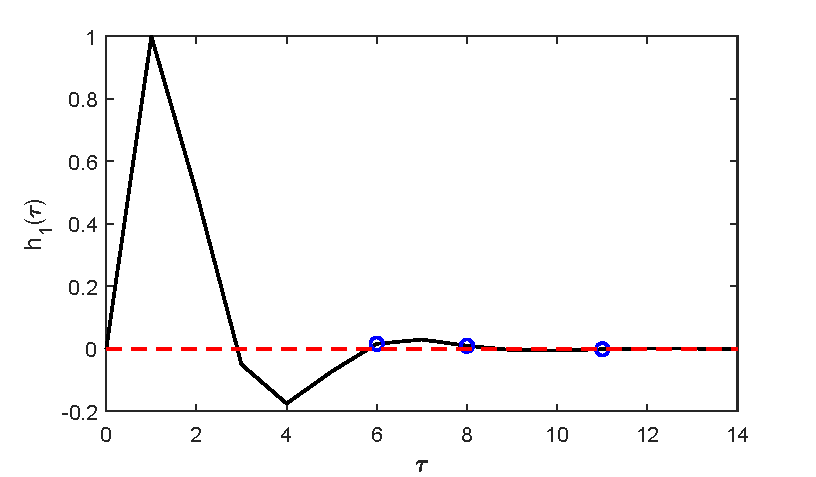
\includegraphics[width = 0.7\textwidth]{Chapter4_EM/LinearKernel_EM.pdf}
\caption{The true first order kernel $h_1$ (black line) in the simulation example, and the three applied truncation lengths (blue circles)}
\label{fig:LinearKernel_EM}
\end{figure}

For both tuning methods, hyperparameters are initialized according to,
%\begin{align*}
%&[\hat{\sigma}^2]^{(0)} = 1.5\sigma^2 \\
%&\hat{c}_m^{(0)} = 1 \; \; \forall \; m, \\
%&[\hat{\lambda}_m^j]^{(0)} = 0.8 \; \; \forall \; m,j.
%\end{align*}
$$ [\hat{\sigma}^2]^{(0)} = 1.5\sigma^2, \; \; \; \hat{c}_m^{(0)} = 1, \; \; \; [\hat{\lambda}_m^j]^{(0)} = 0.8 \; \; \forall \; m,j$$
All non-convex optimizations are performed using $\text{\tt{fmincon}}$ in MATLAB, with a step tolerance of $10^{-3}$. Convergence of the iterative EM method is defined by a change of less than $1\%$ in all hyperparameters. Computation times are measured from the beginning of hyperparameter tuning to convergence, using a PC with Intel Xeon 3.50 GHz processor. In order to observe mean behaviour, each Monte Carlo study considers 10 realizations of each system.

\subsection{Results}

As well as computation time measurements, a validation error metric is calculated for each estimated system by applying a Gaussian validation input of length 20,000 to the estimated and true systems. Labeling the true output as $y_{val}$ and estimated output as $y_{est}$, we construct a normalized RMS error metric defined by,
\begin{equation}
E_{NRMS} = \frac{\text{rms}(y_{val}-y_{est})}{\text{rms}(y_{val})}.
\end{equation}

\renewcommand{\arraystretch}{1.3}
\begin{table}[!h]
\centering
\caption{Mean computation times and validation errors for $n_m = 7$}
\label{Results_nm7}
\begin{tabular}{l||r|r||r|r}
\hline
                & \multicolumn{2}{c||}{\textbf{Mean Comp. Time (s)}} & \multicolumn{2}{c}{\textbf{Mean E\textsubscript{NRMS}}} \\ \cline{2-5} 
\textbf{M} & \hspace{10mm} MLM          & EM            & \hspace{1mm} MLM             & EM            \\ \hline \hline 
1          & 0.064              & 0.173             & 0.249                & 0.224              \\ \hline
2          & 0.132               & 0.389             & 0.189                & 0.187              \\ \hline
3           & 2.848              & 2.114             & 0.176                & 0.161              \\ \hline
4          & 40.10               & 23.13            & 0.133                & 0.135              \\ \hline
5         & 501.9               & 217.7            & 0.117                & 0.114              \\ \hline
\end{tabular}
\end{table}

\renewcommand{\arraystretch}{1.3}
\begin{table}[!h]
\centering
\caption{Mean computation times and validation errors for $n_m = 9$}
\label{Results_nm9}
\begin{tabular}{l||r|r||r|r}
\hline
                & \multicolumn{2}{c||}{\textbf{Mean Comp. Time (s)}} & \multicolumn{2}{c}{\textbf{Mean E\textsubscript{NRMS}}} \\ \cline{2-5} 
\textbf{M} & \hspace{10mm} MLM           & EM            & \hspace{1mm} MLM             & EM            \\ \hline \hline 
1          & 0.071               & 0.269             & 0.218                & 0.203              \\ \hline
2          & 0.229               & 0.778             & 0.148               & 0.148              \\ \hline
3           & 8.704               & 7.761             & 0.123                & 0.120              \\ \hline
4          & 282.6               & 155.3            & 0.089                & 0.101              \\ \hline
5         & 3962              & 1523            & 0.071                & 0.085              \\ \hline
\end{tabular}
\end{table}

\renewcommand{\arraystretch}{1.3}
\begin{table}[!h]
\centering
\caption{Mean computation times and validation errors for $n_m = 12$}
\label{Results_nm12}
\begin{tabular}{l||r|r||r|r}
\hline
                & \multicolumn{2}{c||}{\textbf{Mean Comp. Time (s)}} & \multicolumn{2}{c}{\textbf{Mean E\textsubscript{NRMS}}} \\ \cline{2-5} 
\textbf{M} & \hspace{10mm} MLM           & EM            & \hspace{1mm} MLM             & EM            \\ \hline \hline 
1          & 0.047               & 0.135             & 0.170                & 0.187              \\ \hline
2          & 0.476               & 1.387             & 0.116               & 0.120              \\ \hline
3           & 30.99               & 46.75             & 0.079                & 0.073              \\ \hline
4          & 2799               & 1211            & 0.059                & 0.060              \\ \hline
5         & 80000              & 15720            & 0.040                & 0.062              \\ \hline
\end{tabular}
\end{table}

The mean computation time results shown in Table \ref{Results_nm7} for $n_m = 7$, Table \ref{Results_nm9} for $n_m = 9$, and Table \ref{Results_nm12} for $n_m =12$, demonstrate that a dramatic improvement in computation time scaling is achieved using the proposed EM method for hyperparameter optimization. For the given experimental conditions, estimation time using EM is comparable to MLM tuning at 3rd order, and significantly faster for 4\textsuperscript{th} and higher order systems. The mean validation errors are also provided in the tables, confirming that there is no degradation in model quality. This is not surprising, since the hyperparameters were observed to converge to the same locations for both methods. Figure \ref{fig:EMhyperparams_converging} shows the EM convergence pathway for all hyperparameters in an example 2nd order ($M=2$) realization.

\begin{figure}[h]
\centering
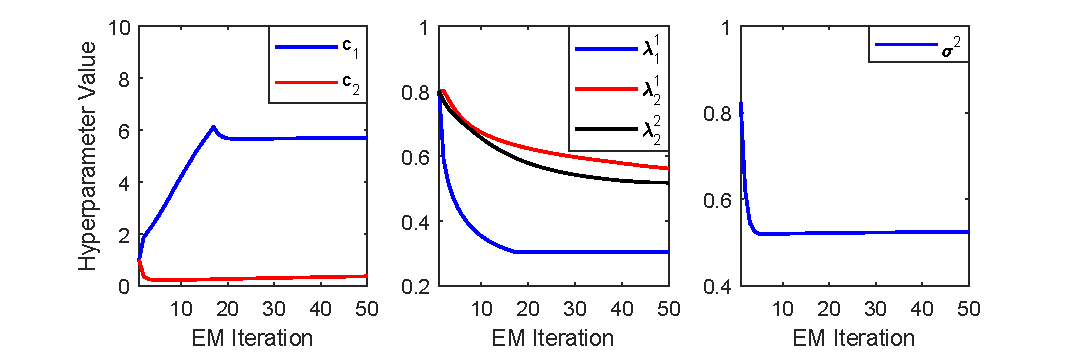
\includegraphics[width = \textwidth]{Chapter4_EM/HyperparamConvergence.pdf}
\caption{EM convergence pathway for all hyperparameters in a 2nd order example}
\label{fig:EMhyperparams_converging}
\end{figure}

To visualize the computation time trend, we label the $M$\textsuperscript{th} order mean computation times as $t_{EM}(M)$ and $t_{MLM}(M)$ for the EM and MLM methods respectively, and define the ratio function, 
\begin{equation}
R(M) = \frac{t_{EM}(M)}{t_{MLM}(M)}.
\end{equation}

$R(M)$ is plotted for all memory lengths in Figure \ref{fig:TimeRatio_EM}. Despite a significant difference in the number of parameters being estimated in each case, the relationship between $R(M)$ and $M$ remains similar, with a crossover point to EM superiority, in terms of computation time, at $M=3 \text{ or } 4$, depending on the memory length. Note that as $n_m$ increases, $R(3)$ increases while $R(M\geq4)$ decreases. The trend predicts increased relative benefit of EM over MLM tuning if $M$ and $n_m$ are increased further. 

\begin{figure}[h]
\centering
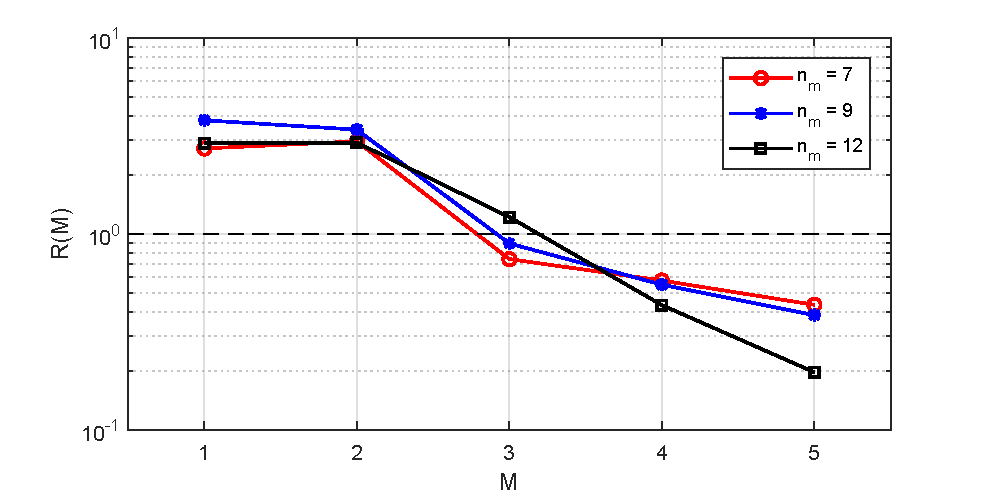
\includegraphics[width = 0.9\textwidth]{Chapter4_EM/Ratios_revised2.pdf}
\caption{Ratios of computation times for varying $M$ and $n_m$}
\label{fig:TimeRatio_EM}
\end{figure}

\section{Conclusion}

Bayesian regularization of Volterra kernel estimates necessitates the optimization of a large number of hyperparameters. When optimizing through a single global marginal likelihood maximization, the computational burden scales rapidly with the order of the Volterra series. In this chapter, the optimization problem was reformulated within an expectation-maximization framework. The new formulation splits the optimization into many small problems, some of which are analytic in nature. The remaining non-convex optimization problems have significantly reduced dimension and do not scale as rapidly with the order of the series. 

Evaluating the MLM and proposed EM-based tuning methods in a Monte-Carlo study revealed improved computation time scaling for the proposed method, with computation time for 4\textsuperscript{th} and 5\textsuperscript{th} order system estimates being significantly lower overall. In the studied example, validation errors obtained using each method's hyperparameters were very similar, and the EM hyperparameters were confirmed to be converging to a maximum of the marginal likelihood function. 

\cleardoublepage
\chapter{Volterra Kernel Identification using Regularized Basis Function Expansions}
\label{chap:5}
\emph{This chapter addresses the feasibility of high order Volterra series estimation from noisy data records, by developing an extension to the Bayesian regularization method which can be applied directly to basis function expansions of the Volterra model. The number of parameters requiring estimation in a basis function expanded model is typically much smaller than for the equivalent time domain series, provided that the basis functions are chosen appropriately for the system. In this chapter, theoretical justification is provided for the proposed approach. The EM algorithm designed in Chapter \ref{chap:4} is then extended to allow the optimization of both the regularization hyperparameters and the basis functions at each nonlinear order of the series. Monte Carlo simulation studies highlight the benefits of a regularized basis function approach over the original time domain method.}
\newpage
\section{Introduction}

The contributions in this part of the thesis are focussed on the challenge of time domain Volterra series identification, and in particular, increasing the feasibility of parameter estimation for high series orders under general experimental conditions. In Chapter \ref{chap:4}, this issue was addressed from the perspective of computation time scaling, where the main optimization was reformulated into a method whose computational burden scales more favourably with series order.

There is another important factor affecting the feasibility of high order estimation, which is the sheer number of parameters required to be estimated in a time domain Volterra model. While the problem is particularly severe in multi-dimensional Volterra kernels, the desire to perform parameter reduction exists also in the linear impulse response case, from which inspiration can be drawn. In particular, orthonormal basis function modeling is a technique traditionally applied to linear systems \cite{Heuberger2005} that has also exhibited significant potential in the nonlinear domain \cite{Cheng2017}.

The use of orthonormal basis functions for linear system identification has been rigorously studied for several decades \cite{Heuberger2005}, \cite{Wahlberg1991}, \cite{Wahlberg1994}. The basic goal is to formulate a compact representation of a linear time-invariant (LTI) system by describing it as a weighted sum of rational orthonormal basis functions.  If the poles of the basis functions are chosen wisely, then only a small number of functions are required to sufficiently model the system behaviour.  Estimating the coefficients of the expansion is a linear-in-the-parameters problem, and the compact structure can produce lower variance estimates at the price of a small bias. Basis function representations are also possible in a Volterra series context \cite{Rugh1980}, however, placement of the basis function poles is more difficult to optimize in multi-dimensional kernels than in the linear case \cite{Campello2004}, \cite{Rosa2007}. 

This chapter makes a novel proposal to combine the parameter reduction technique of basis function modeling with the EM-based regularization method developed in Chapter \ref{chap:4}. By applying regularization directly on the more compact basis function model structure, the variance of model estimates can be dramatically reduced, along with their associated computation time. Theoretical justification is given for the use of regularization on higher-dimensional basis function expansions, and the EM method for hyperparameter tuning is modified to also iteratively optimize the basis function poles at each series order. A Monte Carlo simulation study is performed on example Volterra systems ranging from 2\textsuperscript{nd} to 5\textsuperscript{th} order, to compare the feasibility of high order parameter estimation using the proposed basis function method against the original regularized method in \cite{Birpoutsoukis2017}. 

\section{Orthonormal basis functions in identification}

The motivation for using orthonormal basis functions in linear identification stems directly from the shortcomings of FIR identification \cite{Heuberger2005}.  If we consider the impulse response, $h(\tau)$, generated by the rational transfer function, $G(z)$, we observe that if the poles of $G(z)$ are close to the unit circle, then $h(\tau)$ will tend to 0 very slowly with increasing $\tau$.  This implies that a large number of FIR parameters are required to accurately model the system. If we instead model the system $G(z)$ as a weighted sum of transfer functions $F_i(z)$ with impulse responses $f_i(\tau)$,
\begin{align}
\label{linearBF}
&G(z) = \sum_{i=1}^{\mathcal{B}} \alpha_i F_i(z) \\
\text{and } &h(\tau) = \sum_{i=1}^{\mathcal{B}} \alpha_i f_i(\tau),
\end{align}
with the poles of each $F_i(z)$ chosen carefully, the number of coefficients required to model $G(z)$ can be significantly reduced \cite{Heuberger2005}. 

When choosing a set of basis functions $F_i(z)$, it is desirable that the functions form a complete basis for the subspace of strictly proper, real, rational transfer functions. One class of basis functions which satisfy this criterion are the Takenaka-Malmquist functions \cite{Akcay1998}. The functions are constructed from a sequence of all-pass filters, whose poles, $a_i$, lie within the unit disc and satisfy the completeness condition, $$\sum_{i=1}^{\infty}(1-|a_i|)=\infty.$$ Their general form \cite{Heuberger2005} can be written as 
\begin{equation}
\begin{split}
\label{tak-malm}
F_i(z) &= \frac{\sqrt{1-|a_i|^2}}{z-a_i} \prod_{j=1}^{i-1} \frac{1-\bar{a}_jz}{z-a_j} \\
& = \frac{\sqrt{1-|a_i|^2}}{z-a_i} \prod_{j=1}^{i-1} G_j(z).
\end{split}
\end{equation}

The so-called Generalized Orthonormal Basis Functions (GOBFs) are obtained in the case where $G_j(z) = \bar{G}(z) \; \; \forall j$.  The McMillan degree of $\bar{G}(z)$ can also be made greater than 1, by taking a linear combination of the complex functions generated in (\ref{tak-malm}) \cite{Ninness1997}.  It follows that the total number of generating poles required to define a GOBF sequence is equal to the McMillan degree of $\bar{G}(z)$, which we will denote $d_G$. In the following sections we will examine more closely the case of $d_G =1$ and $d_G = 2$.

\subsection{Laguerre basis functions}
\label{sec:LBFdef}

Laguerre Basis Functions (LBFs) are a subset of the GOBFs which are parameterized by a single, real pole, such that $d_G$ = 1 for the all-pass filter $\bar{G}(z)$. This results in basis functions of the form
\begin{equation}
\label{LBFdef}
F_i(z) = \frac{\sqrt{1-|a|^2}}{z-a} \bigg( \frac{1-a z}{z-a} \bigg) ^{i-1}, \; \; \; a \in (-1,1).
\end{equation}
While the Laguerre functions are easy to construct with a simple structure, one distinct disadvantage is that the functions cannot be constructed using complex poles. As a consequence, a larger number of expansion coefficients are required to accurately model oscillatory systems \cite{Wahlberg1991}.  

\subsection{Kautz basis functions}
\label{sec:KBFdef}

In the case where $d_G = 2$, we can obtain the 2-parameter Kautz Basis Functions (KBFs)~\cite{Wahlberg1994}.  For these functions, the opportunity exists to incorporate a pair of complex poles into the generating all-pass filter in order to better model oscillatory responses.  In much the same way that the Laguerre functions were parameterized by a single real pole in (\ref{LBFdef}), the Kautz functions can be parameterized by two complex conjugate poles,  $[x+iy , x-iy]$. The problem with this parameterization is that the allowable ranges for $x$ and $y$ are interdependent, since $(x^2 + y^2) <1$ is required for stability of $\bar{G}(z)$ \cite{Heuberger2005}.  A more practical parameterization defines two new parameters,
$$a = \frac{2x}{1+x^2+y^2}, \; b = -(x^2+y^2),$$
such that the 2-parameter Kautz functions can be expressed in the form,
\begin{equation}
\begin{split}
\label{KBFdef}
&F_{2i-1}(z) = \frac{\sqrt{1-b^2}(z-a)}{z^2+a(b-1)z-b} \bigg( \frac{-b z^2 + a(b-1)z + 1}{z^2 + a(b-1)z - b} \bigg)^{i-1}, \\
&F_{2i}(z) = \frac{\sqrt{(1-b^2)(1-a^2)}}{z^2+a(b-1)z-b} \bigg( \frac{-b z^2 + a(b-1)z + 1}{z^2 + a(b-1)z - b} \bigg)^{i-1},
\end{split}
\end{equation}
where $a,b \in (-1,1)$. 

\section{Basis function expansions of Volterra models}

Using orthonormal basis functions in a Volterra series model is a concept referred to as the Volterra/Wiener approach \cite{Rugh1980}. In the same way that an impulse response, $h(\tau)$, can be approximated by a sum of basis responses in (\ref{linearBF}), higher-dimensional Volterra kernels can also be approximated using a sum of basis functions.  For a kernel, $h_m(\tau_1,\hdots,\tau_m)$, the basis function expansion can be expressed as
\begin{equation}
\label{OBF2Kernel}
h_m(\tau_1,\hdots,\tau_m) = \sum_{i_1=1}^{\mathcal{B}_m} \hdots \sum_{i_m=1}^{\mathcal{B}_m} \alpha_m(i_1,\hdots,i_m) \prod_{j=1}^{m} f_{m,i_j}(\tau_j), \; \; \; \; m = 1, \hdots, M,
\end{equation}
where $f_{m,l}(\tau)$ is the impulse response corresponding to the $l$\textsuperscript{th} basis function of the kernel $h_m$, $\mathcal{B}_m$ is the number of basis functions in the expansion, and $\alpha_m(\cdot)$ is the set of expansion coefficients. The time domain Volterra series model (\ref{eq:VolterraConvolutionDefn}) can be combined with (\ref{OBF2Kernel}) to restructure the model, i.e.
\begin{equation}
\begin{split}
\label{OBFvolterra}
y^0(t) &= \alpha_0 + \sum_{m=1}^{M} y_m(t), \\
y_m(t) &= \sum_{i_1=1}^{\mathcal{B}_m} \hdots \sum_{i_m=1}^{\mathcal{B}_m} \alpha_m(i_1,\hdots,i_m) \prod_{j=1}^{m} u^f_{m,i_j}(t)
\end{split}
\end{equation}
where $\alpha_0 = h_0$ from (\ref{eq:VolterraTimeDomainOutput}), and $u^f_{m,l}$ is the input, $u$, filtered by the $l$\textsuperscript{th} basis function of the $m$\textsuperscript{th} kernel's basis. Note the similarity in structure between the models in (\ref{eq:VolterraConvolutionDefn}) and (\ref{OBFvolterra}), which motivates the treatment of the expansion coefficient sets $\alpha_m$ as \emph{basis function kernels} in the domains of their corresponding bases. Taking this view, $\mathcal{B}_m$ is analogous to memory length, and the assumption of symmetry, as discussed in Chapter \ref{sec:VolterraProperties}, is equally valid with the same consequences for parameter estimation. The basis function kernels can be much more compact than their time-domain counterparts, provided that the bases are carefully designed \cite{Campello2004},\cite{Rosa2007}. Figure \ref{fig:CompactBFkernel} shows an example 2\textsuperscript{nd} order kernel in the time domain (left) and using a well parameterized LBF expansion (right).

\begin{figure}[h]
\centering
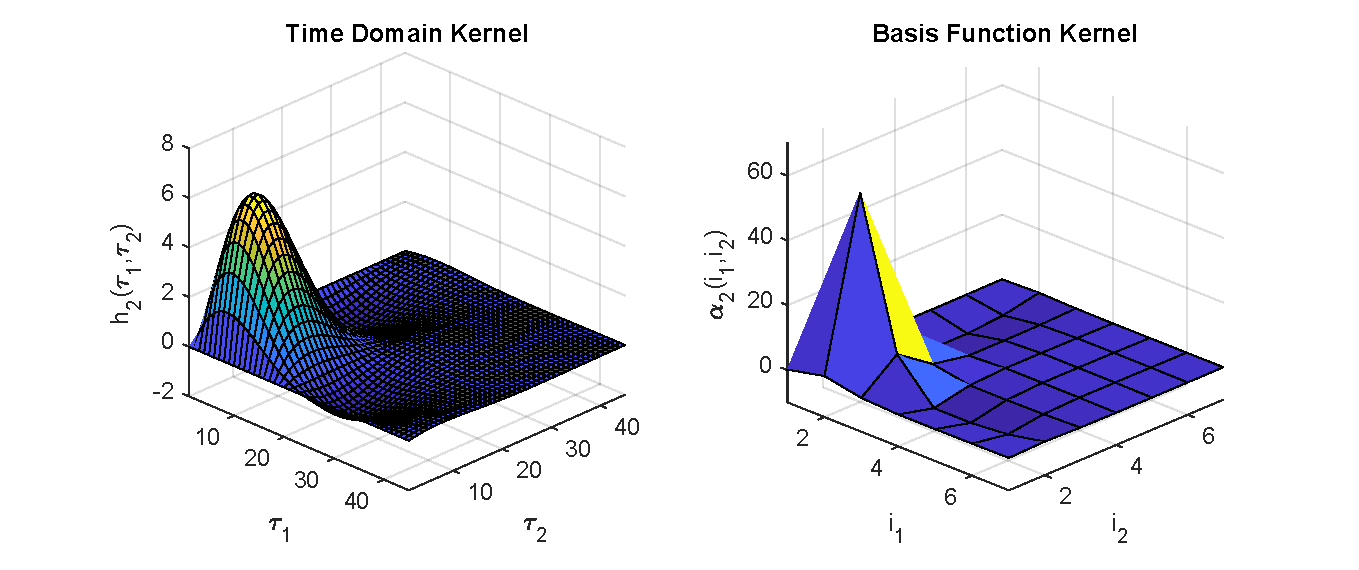
\includegraphics[width = 0.98\textwidth]{Chapter5_RegBFs/TDvsBFkernels3.pdf}
\caption{A well parameterized LBF kernel (right) is typically far more compact than its equivalent time domain kernel (left)}
\label{fig:CompactBFkernel}
\end{figure}

A linear regression formulation for the estimation of the $\alpha_m$ kernels is possible using the same framework described in Chapter \ref{sec:RegVolterraTD}. Based on Assumption \ref{ass:ReLSmodelstructure}, a regression model for the basis function expanded series (\ref{OBFvolterra}) can be given as
\begin{equation}
Y = \Phi_f^T \alpha + E,
\label{eq:RegressionStructure_OBFseries}
\end{equation}
where the regressor, $\Phi_{f}$, now contains appropriate \emph{filtered} input products. The parameter vector is still constructed as if the expansion coefficients $\alpha_m$ were standard Volterra kernels, i.e. $\alpha = [\alpha_0, {\alpha^{\mathcal{V}}_1}^T, \hdots , {\alpha^{\mathcal{V}}_M}^T]^T$, where $\alpha^{\mathcal{V}}_m$ denotes a vector of \emph{unique} $m$\textsuperscript{th} order expansion coefficients.

Naturally a least squares estimate of the basis function kernels is possible, provided that there is enough input/output data available, which is analytically computed using
\begin{equation}
\hat{\alpha}_{LS} = ( \Phi_{f}  \Phi_{f}^T)^{-1} \Phi_{f} Y.
\label{LSbf}
\end{equation}

So far we have assumed that a set of appropriate basis functions exist for each nonlinear order $m$. In reality, these basis functions must be chosen by the user, and ideally the functions for a kernel $h_m$ should reflect the system dynamics present in that kernel. The problem of selecting optimal basis functions for Volterra kernel expansion was considered in \cite{Campello2004} for the case of LBFs, and in \cite{Rosa2007} for the case of KBFs. Optimality here is defined by the minimization of error introduced from truncation of the LBF/KBF expansions to a finite length, $\mathcal{B}_m$. That is to say that an optimal basis will allow the most compact basis function kernel. 

\subsection{Optimal selection of Laguerre poles}
\label{sec:OptimalLBFpole}

We will consider a Volterra kernel $h_m$ of order $m$, which can be expressed as a Laguerre basis function expansion using (\ref{LBFdef}) and (\ref{OBF2Kernel}), parameterized by the pole $a  = a_m$.  It can be shown that minimizing the cost function, 
\begin{equation}
\label{LBFcost}
J_m(a_m) = \sum_{i_1}^{\infty} \hdots \sum_{i_m}^{\infty} (i_1 + \hdots + i_m) \alpha_m^2(i_1, \hdots , i_m),
\end{equation}
with respect to $a_m$ will also minimize the upper bound on the squared norm of the truncation error \cite{Campello2004}. Furthermore, there is a strict global solution to (\ref{LBFcost}) which can be obtained solely from the time-domain kernel.  The optimal pole can thus be calculated from $h_m$ \cite{Campello2004}, i.e.
\begin{equation}
a_m = \frac{2Q_{1,m}-1-Q_{2,m}}{2Q_{1,m}-1+\sqrt{4Q_{1,m}Q_{2,m}-Q_{2,m}^2-2Q_{2,m}}},
\end{equation}
where 
$$Q_{j,m}= \frac{1}{m} \sum_{l=1}^{m} S_{j,l},$$
$$S_{1,l} = \frac{1}{\| h_m \|^2} \sum_{\tau_1=0}^{\infty} \hdots \sum_{\tau_m=0}^{\infty} \tau_l h_m^2(\tau_1, \hdots, \tau_m),$$
$$S_{2,l} = \frac{1}{\| h_m \|^2} \sum_{\tau_1=0}^{\infty} \hdots \sum_{\tau_m=0}^{\infty} \tau_l [\Delta_l h_m(\tau_1, \hdots, \tau_m)]^2,$$
and the operators $\| \cdot \|^2$ and $\Delta_l$ are defined by
$$ \| h_m \|^2 = \sum_{\tau_1=0}^{\infty} \hdots \sum_{\tau_m=0}^{\infty} h_m^2(\tau_1, \hdots, \tau_m),$$
$$ \Delta_l  h_m = h_m(\tau_1, \hdots, \tau_l + 1, \hdots, \tau_m) - h_m(\tau_1, \hdots, \tau_l, \hdots, \tau_m).$$ 

\subsection{Optimal selection of Kautz poles}
\label{sec:OptimalKBFpoles}

For the 2-parameter Kautz case, we consider again the Volterra kernel $h_m$, expanded now using the Kautz functions defined in (\ref{KBFdef}). Unlike the Laguerre case, no analytic solution exists in the literature to find optimal Kautz parameterizations. However, sub-optimal estimates can be obtained by fixing $a = a_m$, as this provides an analytic solution \cite{Rosa2007} for optimizing $b = b_m$ at the given $a_m$ value. Combining this analytic, sub-optimal method with an exhaustive search through the space of valid $a_m$ values will then reveal the global optimum.

It can be shown \cite{Rosa2007} that the upper bound on truncation error resulting from expansion into Kautz functions is minimized by minimizing the cost function,
\begin{equation}
\label{KBFcost}
L_m(a_m,b_m) = \frac{q_2 b_m^2 - 2 q_1 b_m + q_3}{1-b_m^2},
\end{equation}
where the scalars $q_1, q_2, q_3$ are given by
\begin{align*}
&q_1 = \mu_1(g_{even}) + \mu_1(g_{odd}),\\
&q_2 = \mu_2(g_{even}) + \mu_2(g_{odd}),\\
&q_3 = q_2 + m \cdot \mu_3(g_{even}) + m \cdot \mu_3(g_{odd}).
\end{align*}
The moments $\mu_j$ are defined as,
\begin{align*}
\mu_1(g) &= \sum_{j=1}^{m} \Bigg[  \sum_{k_1=0}^{\infty} \hdots \sum_{k_j=0}^{\infty} \hdots \sum_{k_m=0}^{\infty} k_j \cdot g(k_1,\hdots,k_j,\hdots,k_m) \cdot g(k_1,\hdots,k_j-1,\hdots,k_m) \Bigg], \\
\mu_2(g) &= \sum_{j=1}^{m} \Bigg[  \sum_{k_1=0}^{\infty} \hdots \sum_{k_j=0}^{\infty} \hdots \sum_{k_m=0}^{\infty} k_j \cdot g^2(k_1,\hdots,k_m),\\
\mu_3(g) &= \sum_{k_1=0}^{\infty} \hdots \sum_{k_m=0}^{\infty} g^2(k_1,\hdots,k_m),
\end{align*}
and the functions $g_{even}$ and $g_{odd}$ are functions on the time domain kernel:
\begin{align*}
g_{even}(k_1, \hdots, k_m) &= \sum_{\tau_1=0}^{\infty} \hdots \sum_{\tau_m=0}^{\infty} h_m(\tau_1, \hdots, \tau_m) \cdot \prod_{j=1}^{m} \hat{f}_{2k_j+2}(\tau_j),\\
g_{odd}(k_1, \hdots, k_m) &= \sum_{\tau_1=0}^{\infty} \hdots \sum_{\tau_m=0}^{\infty} h_m(\tau_1, \hdots, \tau_m) \cdot \prod_{j=1}^{m} \hat{f}_{2k_j+1}(\tau_j),
\end{align*}
where $\hat{f}_{(\cdot)}$ are the Kautz function impulse responses with $b_m=0$. 

For a fixed value of $a_m$, (\ref{KBFcost}) is convex, and minimized by a specific selection of $b_m$~\cite{Rosa2007}, given by 
\begin{align*}
&b_m^* = 
\begin{cases}
\zeta - \sqrt{\zeta^2-1} &\text{if } \zeta>1, \\
\zeta + \sqrt{\zeta^2-1} &\text{if } \zeta<-1,
\end{cases} \\
\text{where } & \zeta = (q_2 + q_3)/2q_1
\end{align*}
Thus, by searching through a discretized space of $a_m \in (-1,1)$, we can analytically compute the optimal $b_m^*$ for each $a_m$, and the corresponding cost, $L_m(a_m,b_m^*)$. Once the discretized $a_m$-space has been searched, the parameter set which produced a globally minimum $L_m$ is the optimal choice for expansion of $h_m$. 

\section{Regularized identification of basis function kernels}
\label{RegBFs_Chap5}

The parallels between time domain and basis function Volterra models have motivated the treatment of expansion coefficients as \emph{basis function kernels} in the domains of their bases.  A natural progression then is to consider applying regularization to these new kernels in the same way that it was applied to time domain kernels, i.e. by imposing smoothness and decay along the hypersurfaces generated by the basis function expansions.

To this end, one can define a typical quadratically regularized estimator, 
\begin{align}
\label{ReBF}
\hat{\alpha}_{ReLS} &= \text{arg } \underset{\alpha}{\text{min}} \|Y - \Phi_{f}^T \alpha \|^2_2 + \sigma^2 \alpha^T P^{-1} \alpha \\
&= (P \Phi_f \Phi_f^T + \sigma^2 I)^{-1} P \Phi_f Y.
\label{eq:ReBFanalytic}
\end{align}  
As in Chapter \ref{sec:RegVolterraTD}, the penalty matrix $P$ can be constructed block diagonally using Bayesian prior covariances, with the following assumption. 
\begin{assum}
Every vector of expansion coefficients, $\alpha_m^\mathcal{V}$, is a zero mean Gaussian process: 
\begin{equation}
\alpha_m^\mathcal{V} \sim \mathcal{N}(0,P_m) \; \; \; m = 1, \hdots, M.
\end{equation}
Furthermore, all pairs of coefficient vectors, $\alpha_i^\mathcal{V}$ and $\alpha_j^\mathcal{V}$, are independent for $i \neq j$.

The constant offset is also Gaussian, i.e. $\alpha_0 \sim \mathcal{N}(0,P_0)$, and independent of the other processes.
\end{assum}

If we simply frame the basis function kernels as Volterra kernels in a different domain, then the prior covariance for each kernel can be formed via an identical procedure to the time domain case in (\ref{KernelPenalty}), (\ref{TCext})/(\ref{DCext}), and (\ref{FinalPenalty}). Furthermore, the hyperparameters may be tuned using the same EM-based optimization derived in Chapter \ref{chap:4} (Algorithm \ref{alg:EMtuning}). It should be noted, however, that for estimation using basis functions there is an added complication of choosing poles to generate the basis functions at each nonlinear order. These poles can be treated as additional hyperparameters requiring optimization, which requires some modifications to the EM tuning approach.  

\subsection{Theoretical justification}

To impose the same covariance structures on expansion coefficients that have been used on standard Volterra kernel parameters, there must be justification that the basis function kernels will in fact exhibit the same smooth, decaying behaviour. 

For linear FIR models, the concept of regularized basis function estimation has already been explored in \cite{Chen2015}, where the TC covariance structure was applied in regularized estimation of Laguerre coefficients. The approach was shown, in \cite{Darwish2018}, to be equivalent to applying a basis-function-based covariance structure directly on the time-domain FIR parameters. In the linear case, the justification for such an approach is trivial when using Laguerre or Kautz functions. In these cases, the set of expansion coefficients for a (rational) linear system are seen to be the impulse response of the system under a given transformation, where the transformation maps stable poles to other stable poles \cite{Heuberger2005}, \cite{Wahlberg1994}. This implies that the expansion coefficients are also free to be interpreted as a stable impulse response, with all the familiar smoothness and decay properties.   

For higher-dimensional Volterra kernels the linear justification is not applicable, because the definition of stability is more complex (see Chapter \ref{sec:VolterraProperties}), and the notion of poles in some rational linear filter may not exist for an arbitrary nonlinear system. In order to solve this issue, a Bayesian approach is proposed here to show that basis function kernels decay to zero in all causal directions of the hypersurface, so long as their time domain counterparts are well behaved. The approach will be demonstrated for the case of Laguerre basis functions.

\begin{thm}
\label{thm:DecayingLBFs}
If $h_m(\tau_1, \hdots, \tau_m)$ is an $m$\textsuperscript{th} order, zero mean Gaussian Volterra kernel with finite covariance, then any valid Laguerre basis function expansion of the kernel, $\alpha(i_1, \hdots, i_m)$, will decay to 0 in all causal directions.
\end{thm}

\begin{proof*}
Let $i_1 = x_1 s, \hdots, i_m=x_m s$, where $x_1, \hdots, x_m \geq 0$ and $s \to \infty$ is the limit of interest, i.e. we consider the limiting behaviour in some causal direction. 

The infinite basis function expansion is given by
\begin{align}
\alpha(i_1, \hdots, i_m) = \alpha(x_1 s, \hdots, x_m s) = \sum_{\tau_1=0}^{\infty} \hdots \sum_{\tau_m=0}^{\infty} h_m(\tau_1, \hdots, \tau_m) \prod_{j=1}^{m} f_{x_j s}(\tau_j)
\end{align}
where $f_{x_j s}$ is the impulse response for the $x_j s = i_j$\textsuperscript{th} Laguerre function. 

The mean of the expansion coefficients is trivially zero, since $h_m$ is a zero mean process.
The variance of the coefficients is given by
\begin{align}
\label{eq:AlphaVariance}
\Var[\alpha(x_1 s, \hdots, x_m s)] &= \sum_{\tau_1=0}^{\infty} \hdots \sum_{\tau_m=0}^{\infty} \sum_{q_1=0}^{\infty} \hdots \sum_{q_m=0}^{\infty} \nonumber \\ 
&\Cov[h_m(\tau_1, \hdots, \tau_m),h_m(q_1, \hdots, q_m)] \cdot \prod_{j=1}^{m} f_{x_j s}(\tau_j) f_{x_j s}(q_j). 
\end{align}
The Laguerre filters (\ref{LBFdef}) can be rewritten as
\begin{equation}
\label{eq:LongDivResult}
F_i(z)=\frac{0z^i + \sum_{k=0}^{i-1} p_{k,1}(i) a^k z^k}{z^i + \sum_{k=0}^{i-1} p_{k,2}(i) a^{i-k} z^k}, \; \; a \in (-1,1) \setminus \{0\},
\end{equation}
where $p_{m,n}$ are arbitrary polynomials in $i$ resulting from the binomial expansion.
Performing the division in (\ref{eq:LongDivResult}) gives the form for the first $i$ values of $f_i(\tau)$ (See Appendix \ref{append:LongDivision} for the division):
\begin{align*}
f_i(\tau) &= p_{l,j}(i)\cdot a^{i-\tau} \; \; \text{for} \; 0 \leq \tau<i , \; l,j \in \mathbb{Z}^+ \\
&\implies \lim_{i \to \infty} f_i(\tau) = 0\; \; \; \forall \tau \in \mathbb{Z}^+ 
\end{align*}
Hence $s \to \infty$ causes all $ f_{x_j s}(\tau_j), f_{x_j s}(q_j)$ to go to $0$ in (\ref{eq:AlphaVariance}), and since all kernel covariances are finite,
\begin{align*}
&\lim_{s \to \infty} \Var[\alpha(x_1 s, \hdots, x_m s)] = 0 
\end{align*} \qed
\end{proof*}

\begin{rem}
The smoothness of basis function kernels is not addressed in Theorem \ref{thm:DecayingLBFs}, despite being imposed by most common covariance structures. However, if we use the same Bayesian approach on the first order case as an example, the correlation between two expansion coefficients separated by $\epsilon \in \mathbb{Z}^+$ is given by:
$$\textbf{E}\{ \alpha(i) \alpha(i+\epsilon) \} = \sum_{\tau = 0}^{\infty} \sum_{\tau' = 0}^{\infty} \textbf{E}\{h(\tau)h(\tau')\} f_i(\tau) f_{i+\epsilon}(\tau'),$$
which will be nonzero unless $h(\tau)$ was an i.i.d. sequence. This provides the motivation to impose a level of correlation between neighbours, and this level can be tuned by the corresponding hyperparameters.  
\end{rem}

\subsection{Modified EM for pole selection and hyperparameter optimization}

It has been noted that the poles used to generate each Volterra kernel's basis functions must also be optimized to ensure the basis function kernels are as compact as possible. In \cite{Chen2015}, which examined regularized basis function estimation for the linear FIR case, the single Laguerre pole, $a$, was treated as an additional hyperparameter, and placed in the same marginal likelihood optimization routine (\ref{eq:MarginalLikelihood_opt}) used for all other hyperparameters. In the nonlinear case, with multidimensional kernels, it has been shown that a marginal likelihood approach does not scale well with series order, and the addition of extra basis function hyperparameters to the search space would only compound this issue. Instead, the EM method developed in Chapter \ref{chap:4} will be extended here to incorporate the iterative optimization of basis function poles, thereby preserving the computation time benefits associated with an EM approach. 

First, some notational conventions will be clarified. The method will be derived for the case where the TC covariance structure (\ref{TCext}) is used, however it can be adapted to other structures with minimal effort. Collecting all the hyperparameters for the prior covariance matrix, $$\eta_{TC} = [c_0 \; c_1 \; \lambda_1^1 \; c_2 \; \lambda_2^1 \; \lambda_2^2 \; \hdots \; c_M \; \lambda_M^1 \hdots \lambda_M^M],$$ and all the basis-generating parameters, $$\eta_{BF} = \begin{cases} [a_1 \; \hdots \; a_M], & \text{for LBFs} \\ [a_1 \; b_1 \; \hdots \; a_M \; b_M], & \text{for KBFs}\end{cases},$$ we can define the total hyperparameter vector as $\eta = [\eta_{TC} \; \eta_{BF} \; \sigma^2]$. The quantities introduced in Notation \ref{not:decayparams}, \ref{not:decomposedprior} and \ref{not:Wmatrix} will also remain valid here, where time domain parameters $h_m$ and $\theta$ are replaced by the basis function model equivalents, $\alpha_m$ and $\alpha$ respectively. The number of unique kernel coefficients per order, $d_m$, is still computed using (\ref{eq:ParametersPerKernel}), where $n_m$ is replaced by $\mathcal{B}_m$.

As summarized in Sections \ref{sec:OptimalLBFpole} and \ref{sec:OptimalKBFpoles}, optimal selection of the LBF/KBF poles requires exact knowledge of the time-domain kernels, $h_m$. Since the kernels are the quantities we are required to estimate, we will instead embed the pole optimization as an additional step in the recursive EM method, such that poles are computed at each iteration which are `optimal' for the regularized kernel estimates obtained using the current hyperparameter guess. The specific implementation details for this modified EM approach are outlined in Algorithm \ref{alg:BFopt}, where $\eta_{TC}$ and $\sigma^2$ are optimized using the same methods introduced in Chapter \ref{chap:4}, and $\eta_{BF}$ is also iteratively updated inside the loop using the relevant results from either \cite{Campello2004} (LBFs) or \cite{Rosa2007} (KBFs). 

\begin{algorithm}[h]
\begin{algorithmic}[1]
\Require $N$ input samples, $Y$, initial hyperparameter guess $\hat{\eta}^{(0)}$, and tolerance $\epsilon$
\State $k \gets 0$
\While{$\text{max}(|\hat{\eta}^{(k)}-\hat{\eta}^{(k-1)}|/|\hat{\eta}^{(k-1)}|) > \epsilon$}
\State Form $\phi_{f}(\eta_{BF})$ using $\hat{\eta}_{BF}^{(k)}$
\State Form $P$, $\textbf{E} \{ \alpha \}$ and $\textbf{E} \{ \alpha \alpha^T \}$ using $\hat{\eta}^{(k)}$
\ForAll{$m \in 0,1,\hdots,M$}
\State Extract $\bar{P}_m$ from $P$ and $W_m$ from $\textbf{E} \{ \alpha \alpha^T \}$
\If{m>0} 
	\State Compute $\hat{\bar{\eta}}_m^{(k+1)}$ using (\ref{eq:decay_update})
\EndIf
\State Compute $\hat{c}_m^{(k+1)}$ using (\ref{eq:constant_update})
\EndFor
\State Compute $[\sigma^2]^{(k+1)}$ using (\ref{eq:noisevar_update})
\State Compute $\hat{\alpha}_{ReLS}^{(k+1)} = \textbf{E} \{ \alpha \}$ using $\big[\hat{\eta}_{TC}^{(k+1)} \; [\sigma^2]^{(k+1)}\big]$
\State Convert $\hat{\alpha}_{ReLS}^{(k+1)}$ to time domain kernel estimates $\{\hat{h}^{(k+1)}_m\}_{m=0}^{M}$ using (\ref{OBF2Kernel})
\State Compute `optimal' basis generating parameters $\hat{\eta}_{BF}^{(k+1)}$ from $\{\hat{h}^{(k+1)}_m\}_{m=1}^{M}$ (see Section \ref{sec:OptimalLBFpole} (LBFs) or \ref{sec:OptimalKBFpoles} (KBFs))
\State $k \gets k+1$
\EndWhile
\State \textbf{return} $\hat{\eta}^{(k)}$
\end{algorithmic}
\caption{EM-based hyperparameter tuning for basis function Volterra kernels}
\label{alg:BFopt}
\end{algorithm}

One desirable property of traditional EM methods is their guaranteed convergence to a stationary point of the marginal likelihood function, $L(Y;\eta)$. The result in Theorem \ref{thm:ModEMConvergence} shows that this property is essentially maintained in Algorithm \ref{alg:BFopt}.
\begin{thm}
\label{thm:ModEMConvergence}
The sequence, $\hat{\eta}^{(k)}$, generated by Algorithm \ref{alg:BFopt} will converge to a stationary point of the marginal likelihood function $L(Y;\eta)$, provided that $$\exists j \in \mathbb{Z}^+: \forall k \geq j, \; \; \hat{\eta}_{BF}^{(k)} = \hat{\eta}_{BF}^{(k+1)},$$ i.e. the basis function parameters converge before the total sequence converges.
\end{thm}
\begin{proof*}
After iteration $j$, we can define a new sequence $\hat{\eta}_*^{(l)}$ where $\hat{\eta}_*^{(0)}$ = $\hat{\eta}^{(q)}$ and $l = k-j$. It is clear that the new sequence, $\hat{\eta}_*^{(l)}$, corresponds to a fixed (basis function) model structure, $$Y = \phi_{f}^T(\hat{\eta}_{BF}^{(j)}) \alpha + E,$$ and is therefore a standard EM sequence as in Chapter \ref{chap:4} (Algorithm \ref{alg:EMtuning}). Thus, the new sequence converges to a stationary point of $L(Y;\eta)$ \cite{Wu1983}, and so must the original, $\hat{\eta}^{(k)}$. \hfill \qed
\end{proof*}

\subsection{Computational complexity and parameter reduction}

In the context of regularized Volterra series estimation, the main benefit of a basis function formulation over the original time domain approach is the potential for a dramatic reduction in the number of parameters required for an accurate model. More specifically, one would expect the length, $\mathcal{B}_m$, of a basis function kernel to be much smaller in general than the equivalent time domain memory length, $n_m$. Considering a generic $m$\textsuperscript{th} order kernel with length $q$, the number of unique parameters requiring estimation was given in (\ref{eq:ParametersPerKernel}), i.e.  
$$d_m = \frac{\prod_{j=0}^{m-1}(q+j)}{m!},$$
and thus $d_m$ grows as $\mathcal{O}(q^m)$. It is clear that even a small difference between $\mathcal{B}_m$ and $n_m$ can imply a large difference in the \emph{total} number of parameters required, especially as the order, $m$, is increased. 

A reduction in the number of parameters being estimated will also impact on the computation time (and memory requirements) for the estimator. Computation time scaling is hard to define with respect to the number of parameters, due to the non-convex optimization problems involved in Algorithm \ref{alg:BFopt}, however the largest matrix computations scale as $\mathcal{O}\big((\sum_{m=0}^{M} d_m)^3\big)$, such that smaller parameter numbers imply \emph{much} lower computation times.

\section{Numerical examples}

A number of Monte Carlo simulation studies are conducted to evaluate the performance of the proposed regularized basis function method for Volterra kernel identification. The studies are performed on systems with disparate dynamics, to emphasize the different advantages of Kautz and Laguerre bases. The basis function methods also permit estimation of higher order kernels than their time-domain counterpart, due to the compact nature of basis function representations, and this is demonstrated via third, fourth and fifth order systems.

\subsection{Simulation Settings}

In similar fashion to Chapter \ref{chap:4}, the test systems are given by a Wiener-type structure,
\begin{equation}
y(t) = \sum_{m=1}^M \bigg( \frac{N_m q^{-1}}{A(q)}u(t)\bigg)^m +e(t),
\end{equation}   
where $q^{-1}$ is the backwards shift operator, and $e(t) \sim \mathcal{N}(0,\sigma^2)$ is Gaussian output noise added in each realization. Each term in the sum defines an $m$\textsuperscript{th} order Volterra kernel (see Chapter \ref{sec:BlockStructureRelationship}), and each kernel possesses the same denominator dynamics, with $N_m \in \mathbb{R}^+$ scaling the kernel's contribution to the output. The constant offset term is neglected.

The simulation studies differ both in the resonance of the underlying linear filter, as well as the maximum kernel order, $M$. Two second order ($M=2$) systems are tested, with their dynamics given by
\begin{align*}
&\textbf{Sys2a: } A(q) = 1-1.8036q^{-1}+0.8338q^{-2}, \\ 
&\textbf{Sys2b: } A(q) = 1-1.5q^{-1}+0.8125q^{-2}.
\end{align*}
`Sys2a' is lightly underdamped, while `Sys2b' has a significantly lower damping ratio. Studies are also performed on three higher order systems, `Sys3' ($M=3$), `Sys4' ($M=4$) and `Sys5' ($M=5$), which use the same underlying filter as Sys2a, with approximately equal contributions to the output from each kernel (scaled using $N_m$). The impulse response for each of the underlying linear filters can be seen in Figure \ref{fig:Sys2a2bLinear}. 
\begin{figure}[!h]
\centering
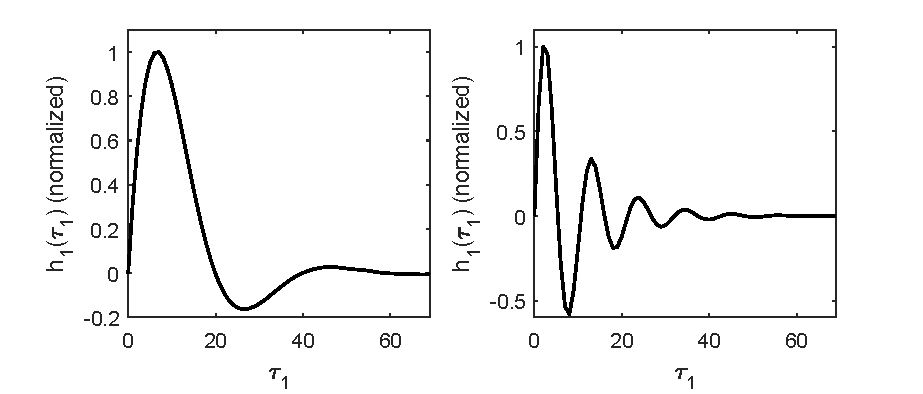
\includegraphics[width = 0.75\textwidth]{Chapter5_RegBFs/Sys2a2b_h1.pdf}
\caption{Normalized impulse response of the linear filter for Sys2a/Sys3/Sys4/Sys5 (left) and Sys2b (right)}
\label{fig:Sys2a2bLinear}
\end{figure}
The corresponding optimal basis function expansions are plotted in Figure \ref{fig:Sys2a2bBF} up to $i_1 = 10$. It is clear for Sys2b that a KBF expansion is the more suitable choice, since the resonant behaviour can be captured in a more compact set of basis functions.
\begin{figure}[!h]
\centering
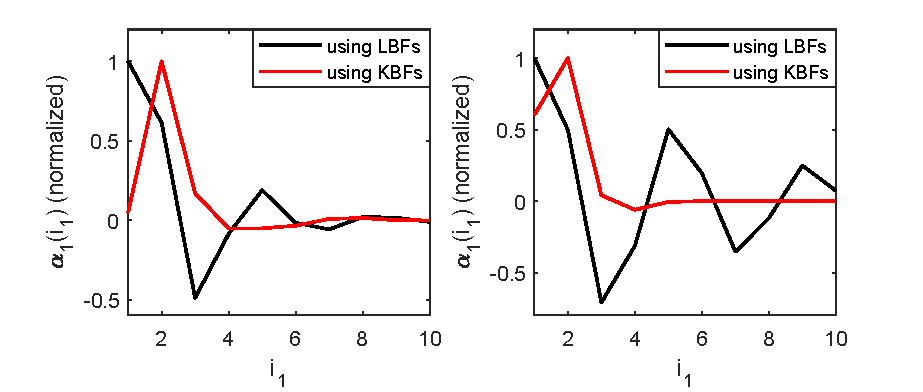
\includegraphics[width = 0.75\textwidth]{Chapter5_RegBFs/Sys2a2b_alpha1.pdf}
\caption{Normalized optimal LBF/KBF expansion coefficients of the linear filter for Sys2a/Sys3/Sys4/Sys5 (left) and Sys2b (right)}
\label{fig:Sys2a2bBF}
\end{figure}

For each system and method, Monte Carlo studies are performed at Signal to Noise Ratios (SNR) of 20dB and 5dB, with 100 realizations per setting. The input, $u$, is constructed as a white Gaussian signal, $u(t) \sim \mathcal{N}(0,1)$, and the data length chosen to be $N=3412$; only 30\% longer than the minimum least squares requirement for Sys2a and Sys2b.

The methods proposed in this chapter are evaluated alongside their unregularized basis function counterparts, as well as a direct time-domain approach. Note that for high nonlinear orders ($M>2$), it is not possible to evaluate the time domain approach due to its immense computational requirements. The details of each method are:

\begin{enumerate}
\item \textbf{ReLS}: The Bayesian regularized method from \cite{Birpoutsoukis2017} in the time domain, using the TC covariance structure in (\ref{KernelPenalty}), (\ref{TCext}) and (\ref{FinalPenalty}), and tuned using MLM. 
\item \textbf{LBF}/\textbf{KBF}: Least squares estimation of LBF/KBF coefficients using (\ref{LSbf}). Optimal basis-generating hyperparameters are assumed to be known a priori (an oracle assumption).
\item \textbf{ReLBF}/\textbf{ReKBF}: Regularized estimation of LBF/KBF kernels using the proposal (\ref{eq:ReBFanalytic}) and the modified EM approach in Algorithm \ref{alg:BFopt} for hyperparameter tuning and pole selection. 
\end{enumerate}

The time domain method is required to estimate each kernel up to a memory length $n_m=70$, while the basis function methods used a length of $\mathcal{B}_m = 10$. For ReLBF/ReKBF, the optimization tasks in Algorithm \ref{alg:BFopt} are performed using MATLAB's $\text{\tt{GlobalSearch}}$ and $\text{\tt{fmincon}}$ functions, and the iterative procedure is terminated when within a 0.5\% convergence tolerance on all hyperparameters. 

For each method and order, Table \ref{tab:ParamNos_OBFS} shows the calculated number of unique kernel parameters to be estimated, $n_p$, and the total number of hyperparameters, $n_h$. From the table, it is clear that for Sys3, Sys4 and Sys5, ReLS requires an unreasonably high number of parameters, and will become too computationally intensive to be feasible. Hence, we consider only LBF and ReLBF methods for these cases. 

\begin{table}[h]
\centering
\caption{Number of parameters ($n_p$) and hyperparameters ($n_h$) for each method and order}
\label{tab:ParamNos_OBFS}
\begin{tabular}{c|c||ccccc}
\multicolumn{2}{r}{Method:}                                                & ReLS & LBF & KBF & ReLBF & ReKBF \\ \hline \hline
\multirow{2}{*}{\begin{tabular}[c]{@{}l@{}}2nd\\ order\end{tabular}} & $n_p$ &2555 &65 &65 &65 &65 \\
                                                                     & $n_h$ &6 &0 &0 &8 &10 \\ \hline
\multirow{2}{*}{\begin{tabular}[c]{@{}l@{}}3rd\\ order\end{tabular}} & $n_p$ &62,195      &285     &285    &285      &285      \\
                                                                     & $n_h$ &10      &0     &0     &13       &16       \\ \hline
\multirow{2}{*}{\begin{tabular}[c]{@{}l@{}}4th\\ order\end{tabular}} & $n_p$ &1,150,625      &1000     &1000    &1000      &1000       \\
                                                                     & $n_h$ &15      &0     &0     &19       &23   \\ \hline   
\multirow{2}{*}{\begin{tabular}[c]{@{}l@{}}5th\\ order\end{tabular}} & $n_p$ &17,259,389      &3002     &3002    &3002      &3002       \\
                                                                     & $n_h$ &21      &0     &0     &26       &31  
\end{tabular}
\end{table}

\subsection{Results}

For each Monte Carlo study, the estimation errors are quantified with the same validation error metric used in \cite{Birpoutsoukis2017}, calculated by applying a validation input of length 50,000 to both the true system and the estimated system and defining `normalized RMS error' as,
\begin{equation}
E_{NRMS} = \frac{\textrm{rms}(y_{val}-y_{mod})}{\textrm{rms}(y_{val})},
\end{equation}
where $y_{val}$ and $y_{mod}$ are the noise-less outputs of the true and estimated system respectively. 

The second order results, presented as boxplots in Figures \ref{Sys2a_Val} and \ref{Sys2b_Val}, show significant improvements in output prediction using ReLBF and ReKBF. The advantage of Kautz functions for resonant systems is clear in the Sys2b (low damping) results, with ReKBF outperforming all other methods. The unregularized estimates do not perform as well, despite being provided with optimal basis functions prior to identification.

\begin{figure}[!h]
\centering
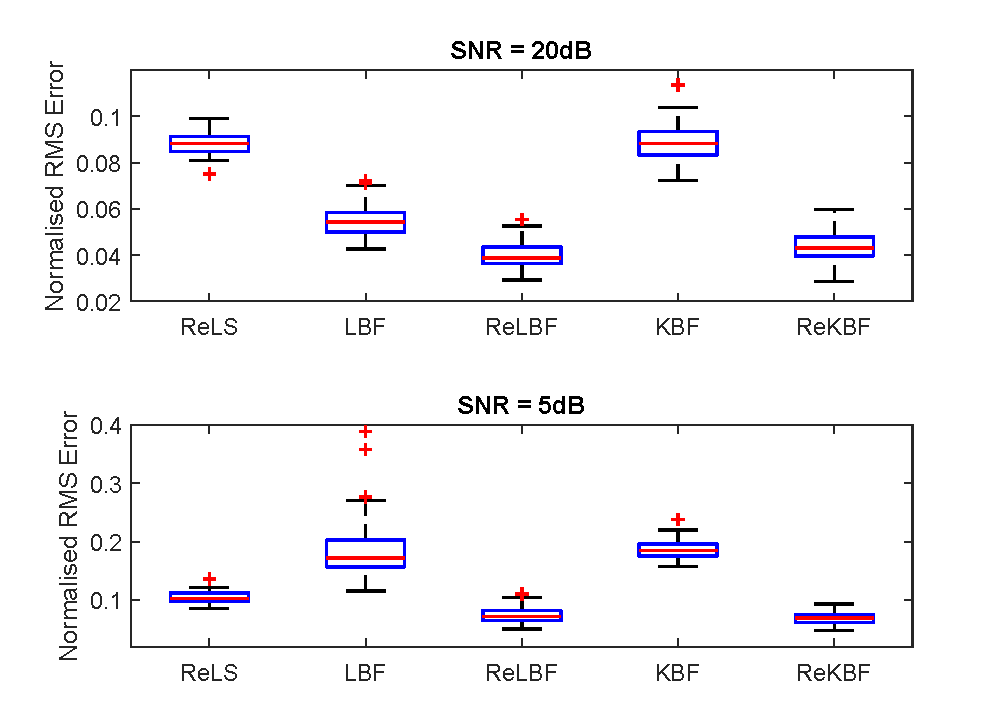
\includegraphics[width = 0.7\textwidth]{Chapter5_RegBFs/Georgios_2ndOrder.pdf}
\caption{Validation errors for Sys2a with SNR = 20dB (top) and 5dB (bottom)}
\label{Sys2a_Val}
\end{figure}

\begin{figure}[!h]
\centering
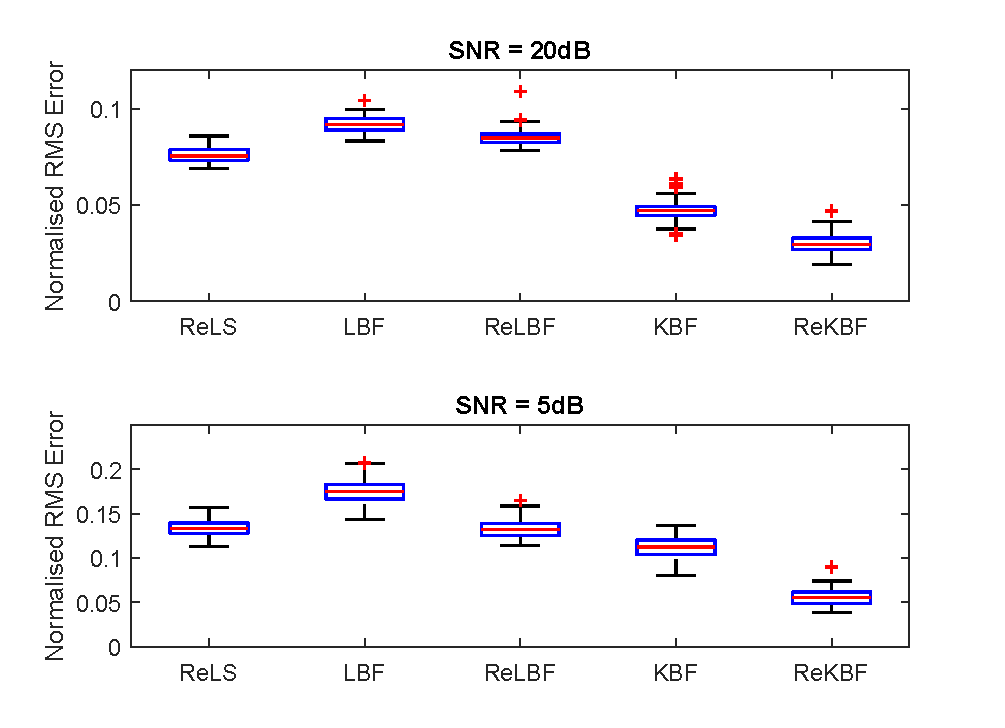
\includegraphics[width = 0.7\textwidth]{Chapter5_RegBFs/Resonant_2ndOrder.pdf}
\caption{Validation errors for Sys2b with SNR = 20dB (top) and 5dB (bottom)}
\label{Sys2b_Val}
\end{figure}

%\begin{table}[t]
%\centering
%\caption{Mean computation times and parameter numbers for 2nd order estimates}
%\label{tab:MeanCompTimes_OBFs}
%\begin{tabular}{c|rrrrr}
%Method & ReLS  & LBF & KBF  & ReLBF & ReKBF \\ \hline
%Time (s) & 375.8 & 0.8 & 1.7 & 37.2  & 53.5 \\
%$n_p$ &2555 &135 &135 &135 &135 \\
%$n_h$ &6 &0 &0 &8 &10
%\end{tabular}
%\end{table}

The validation errors for Sys3, Sys4 and Sys5 are given in Figures \ref{Sys3_Val}, \ref{Sys4_Val} and \ref{Sys5_Val} respectively, which highlight the benefit of the regularized basis function method in lowering model error to tolerable levels. The time domain method, ReLS, requires unreasonably high numbers of parameters and hence is computationally unfeasible. The least squares LBF model estimates, while computationally tractable, produce extremely innacurate predictions. The newly proposed regularized method, however, obtains estimates with reasonable accuracy and computation time using a standard computer architecture, which would not previously have been possible with existing estimation methods under these experimental conditions. For comparison, mean computation times are provided, in Table \ref{tab:MeanCompTimes_OBFs}, for the attempted methods at each order. 

\begin{figure}[!h]
\centering
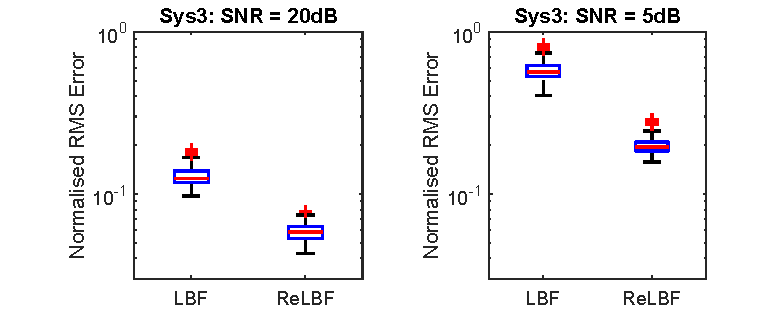
\includegraphics[width = 0.7\textwidth]{Chapter5_RegBFs/Georgios_3rdOrder.pdf}
\caption{Validation errors for Sys3 with SNR = 20dB (left) and 5dB (right)}
\label{Sys3_Val}
\end{figure}
\begin{figure}[!h]
\centering
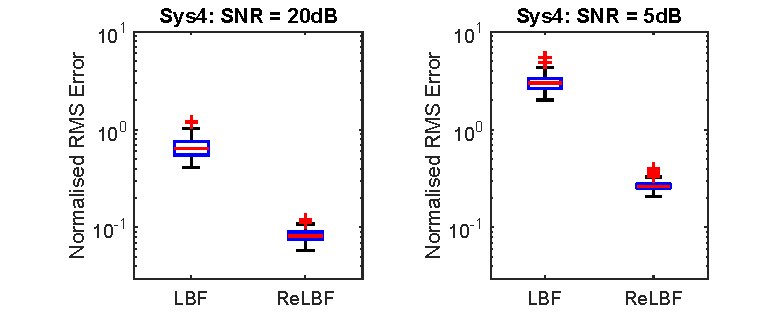
\includegraphics[width = 0.7\textwidth]{Chapter5_RegBFs/Georgios_4thOrder.pdf}
\caption{Validation errors for Sys4 with SNR = 20dB (left) and 5dB (right)}
\label{Sys4_Val}
\end{figure}
\begin{figure}[!h]
\centering
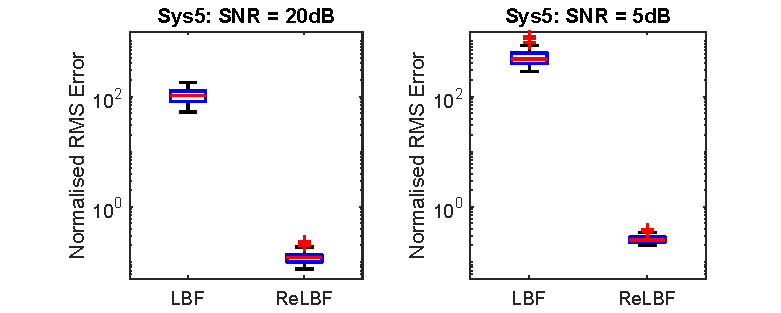
\includegraphics[width = 0.7\textwidth]{Chapter5_RegBFs/Georgios_5thOrder.pdf}
\caption{Validation errors for Sys5 with SNR = 20dB (left) and 5dB (right)}
\label{Sys5_Val}
\end{figure}
\begin{table}[!h]
\centering
\caption{Mean computation time (s) for each method and order}
\label{tab:MeanCompTimes_OBFs}
\begin{tabular}{c||ccccc}
\multicolumn{1}{r}{Method:}                                              & ReLS & LBF & KBF & ReLBF & ReKBF \\ \hline \hline
2nd order	& 376 & 0.4 & 0.9 & 22  & 32 \\
3rd order &-&0.7&-&48&- \\
4th order	&-&1.3&-&228&- \\
5th order	&-&4.3&-&3687&- \\
\end{tabular}
\end{table}

\section{Conclusion}

This chapter makes a novel proposal to combine the techniques of Bayesian regularization and basis function modeling for the purpose of Volterra series estimation. Some theoretical motivation is provided for imposing standard covariance structures on the resultant basis function kernels, and a modified EM algorithm is constructed as an extension of the results in Chapter \ref{chap:4}. The extended algorithm is capable of optimizing both the covariance hyperparameters and the basis-generating hyperparameters, and the iterative procedure will scale more favourably with series order than a direct marginal likelihood approach. The performance of the proposed estimation method has been compared against unregularized least squares estimates, and estimates directly in the time domain, with improved output prediction in all test cases. Furthermore, under the experimental conditions considered in the simulation examples, the proposed method allowed access to computationally feasible and accurate estimates at higher series orders than was previously possible with existing methods in the literature. 

Regularized basis function estimation is clearly a promising tool in addressing the major challenge of time domain Volterra series identification: accuracy and computational feasibility for high order models under arbitrary experimental conditions. 

%There is still work which can be done in this area, for example in exploring the convergence properties of the modified EM Algorithm \ref{alg:BFopt}, which does not become a traditional EM sequence until the basis generating hyperparameters converge. The method can also be extended to other sets of basis functions, particularly those which have already found success in unregularized Volterra series problems.  

\begin{subappendices}
\section{Long division of Laguerre basis function filters}
\label{append:LongDivision}

For a rational transfer function in the $z$-domain, performing a polynomial long division between the numerator and denominator will produce the corresponding impulse response. For example, long division of the transfer function $\frac{1}{z-p}$ for some pole $p \in \mathbb{R}$ will produce
\begin{equation}
0 + 1z^{-1} + p z^{-2} + p^2 z^{-3} + \hdots + p^{i-1} z^{-i} + \hdots,
\end{equation}
where the sequence of coefficients, $[0, 1, p, p^2, \hdots, p^{i-1}, \hdots]$, is the impulse response.

The same process is now applied to the arbitrary order Laguerre filter in (\ref{eq:LongDivResult}), to reveal the structure of the filter's impulse response: 
\begin{sidewaystable}

\small

\begin{alignat*}{9}
&\mathbf{0} &+ &\mathbf{\big[p_{i-1,1}(i) a^{i-1} \big]}z^{-1} &+&\mathbf{\big[p_{i-1,4}(i) a^{i-2}\big]} z^{-2} &+&\mathbf{\big[p_{i-1,8}(i) a^{i-3}\big]} z^{-3} &+ &\hdots \\ \cline{2-10} 
z^i + \sum_{k=0}^{i-1} p_{k,2}(i) a^{i-k} z^k \smash{\Bigg)} &0z^i &+ &\sum_{k=0}^{i-1} p_{k,1}(i) a^k z^k & & & \\
&0 &+ &0 &&&&&&	\tag{end of step 0}\\ \cline{3-10} 
&&  &\sum_{k=0}^{i-1} p_{k,1}(i) a^k z^k &&&&&&  \tag{remove $i-1$ from sum}\\
&&= &p_{i-1,1}(i) a^{i-1} z^{i-1} &+ &\sum_{k=1}^{i-1} p_{k-1,1}(i) a^{k-1} z^{k-1} &&&& \tag{extract $f_i(1)$ and multiply out}\\
&& &p_{i-1,1}(i) a^{i-1} z^{i-1} &+ &\sum_{k=1}^{i-1} p_{k-1,3}(i) a^{2i-k-1} z^{k-1} &+ &\hdots && \tag{end of step 1}\\ \cline{5-10} 
&& & & &\sum_{k=1}^{i-1} (p_{k-1,1}(i) - p_{k-1,3}(i)a^{2i-2k}) a^{k-1} z^{k-1} &+ &\hdots \tag{remove $i-1$ from sum}\\
&&& &= &p_{i-1,4}(i)a^{i-2}z^{i-2} &+ &\sum_{k=2}^{i-1} (p_{k-2,1}(i) - p_{k-2,5}(i)a^{2i-2k}) a^{k-2} z^{k-2} &+ &\hdots \\
&&& & &p_{i-1,4}(i)a^{i-2}z^{i-2} &+ &\sum_{k=2}^{i-1} p_{k-2,6}(i)a^{2i-k-2} z^{k-2} &+ &\hdots \tag{end of step 2}\\ \cline{7-10} 
&&& & & & &\sum_{k=2}^{i-1} (p_{k-2,1}(i)-p_{k-2,7}(i)a^{2i-2k})a^{k-2} z^{k-2} &+ &\hdots \\
&&& & & &= &p_{i-1,8}(i)a^{i-3} z^{i-3} &+ &\sum_{k=3}^{i-1} \hdots \\
&&& & & & &p_{i-1,8}(i)a^{i-3} z^{i-3} &+ &\sum_{k=3}^{i-1} \hdots \\ \cline{9-10}  \\
&&& & & & & \text{and so on up to step $i-1$} 
\end{alignat*}

\normalsize

\end{sidewaystable}

\end{subappendices}


\cleardoublepage
\chapter{Practical Case Studies in Time Domain Identification}
\label{chap:6}
\emph{In this chapter, the theoretical contributions of Chapters \ref{chap:4} and \ref{chap:5} are evaluated on experimental data obtained from nonlinear benchmark systems in the identification community. Firstly, Volterra series model estimates are obtained for a cascaded water tanks system using the regularized basis function approach, with accuracy and computation time compared against the equivalent time domain method. Following this, the same basis function method is applied to a coupled electric drives system to estimate a second order Volterra model. The validation performance of this model is compared against other popular linear and nonlinear model classes estimated using the MATLAB System Identification Toolbox.}
\newpage
\section{Introduction}

Monte Carlo simulations are a useful tool for the analysis of estimation methods, however it is difficult to replicate all of the complexities which feature in a real world identification problem. The numerical examples in Chapters 4 and 5 revealed many favourable properties of the techniques proposed in this thesis, but the simulations relied on an artificially constructed true system which was in the correct model class, had a known maximum nonlinear order, and was disturbed only by measurement noise of the correct Gaussian distribution. Such ideal conditions are never present in practice, and therefore it is important to evaluate the estimation methods in a practical setting as well.

In this chapter, we will consider the estimation of Volterra series models for two real system examples. Both systems are part of a set of established nonlinear benchmark problems used within the system identification community. The first system is known as the cascaded tanks benchmark \cite{Schoukens2016c}, while the second is referred to as the coupled electric drives \cite{Wigren2017}. Note that the full set of benchmark problems can be found at \url{www.nonlinearbenchmark.org}. 

In keeping with the motivation for this part of the thesis, the experimental conditions in both benchmark problems pose a significant challenge for identification of Volterra series models due to the extremely short data records available for estimation. The regularized basis function approach with EM tuning, proposed in Chapter \ref{chap:5}, will be examined for each benchmark and compared against existing methods in the literature.  

\section{Cascaded tanks}

The cascaded tanks benchmark \cite{Schoukens2016c} is a system concerned with fluid level control, which is a common control problem in process industries. Model estimation for the total system is a challenging task due to a number of factors, including combined weak and hard nonlinear dynamics, process noise, unknown initial conditions and a short estimation data record. While there have been several successful grey-box modeling attempts (see e.g. \cite{Pan2018}) which consider the fluid dynamics and process noise directly, in this chapter the identification problem will be undertaken without the use of any prior knowledge, since this is the strength of a nonparametric Volterra series approach. More specifically, the computational burden and prediction accuracy of regularized basis function estimation will be assessed and compared against equivalent estimates obtained using the regularized time domain method in \cite{Birpoutsoukis2017}, which was applied to the cascaded tanks benchmark in \cite{Birpoutsoukis2017b}. 

\subsection{System description}

The system consists of two vertically cascaded tanks, each with small valve openings in the bottom. The top tank is fed with water via a pump which is controlled by a voltage. Water flows through a valve in the top tank to the bottom tank, and through a valve in the bottom tank to a reservoir underneath. The height of the water in the lower tank is the output of the system, measured in volts by a noisy, uncalibrated capacitive sensor. The process is shown in Figure \ref{fig:System_Tanks}. 

\begin{figure}[h]
\centering
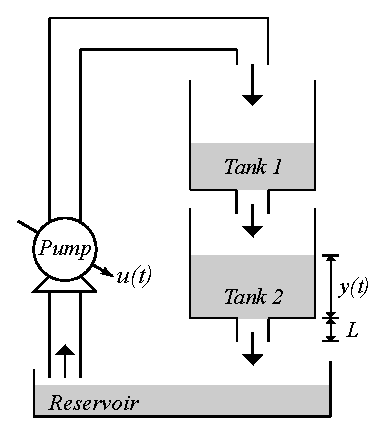
\includegraphics[width=0.48\textwidth]{Chapter6_CaseStudies/TanksSchematic.pdf}
\caption{Diagram of cascaded tanks benchmark system with typical water flow}
\label{fig:System_Tanks}
\end{figure}

Ignoring saturation, the system is weakly nonlinear based on the flow equations through the valves in each tank, which can be derived from Bernoulli's principle. The system also contains a hard nonlinearity in the form of water level saturation. Once the maximum level of either tank is reached, an overflow occurs. Furthermore, saturation in the top tank introduces input-dependent process noise, since some of the overflowing water can fall into the lower tank and affect the output. 

\subsection{Measurement process}

Two sets of data have been recorded for the benchmark: an estimation set and a validation set. For both datasets, the voltage input to the tank system is excited using one period of a multisine which excites frequencies from 0 to 0.0144 Hz. Using a sampling period of $T_s=4$s, this gives input vectors of length $N=1024$. The corresponding output measurements are obtained from the capacitive level sensor of the lower tank, which may introduce measurement noise. The system is not in steady state during the measurement window, and the initial states of the system are unknown but approximately equal for both datasets. The recorded signals are plotted in Figure \ref{fig:datasets_tanks} in the time domain (top) and frequency domain (bottom). While the hard saturation nonlinearity is clearly visible in the time domain output signals, there is also evidence of nonlinearity in the frequency domain, where some output power exists at unexcited frequencies.

\begin{figure}[h]
\centering
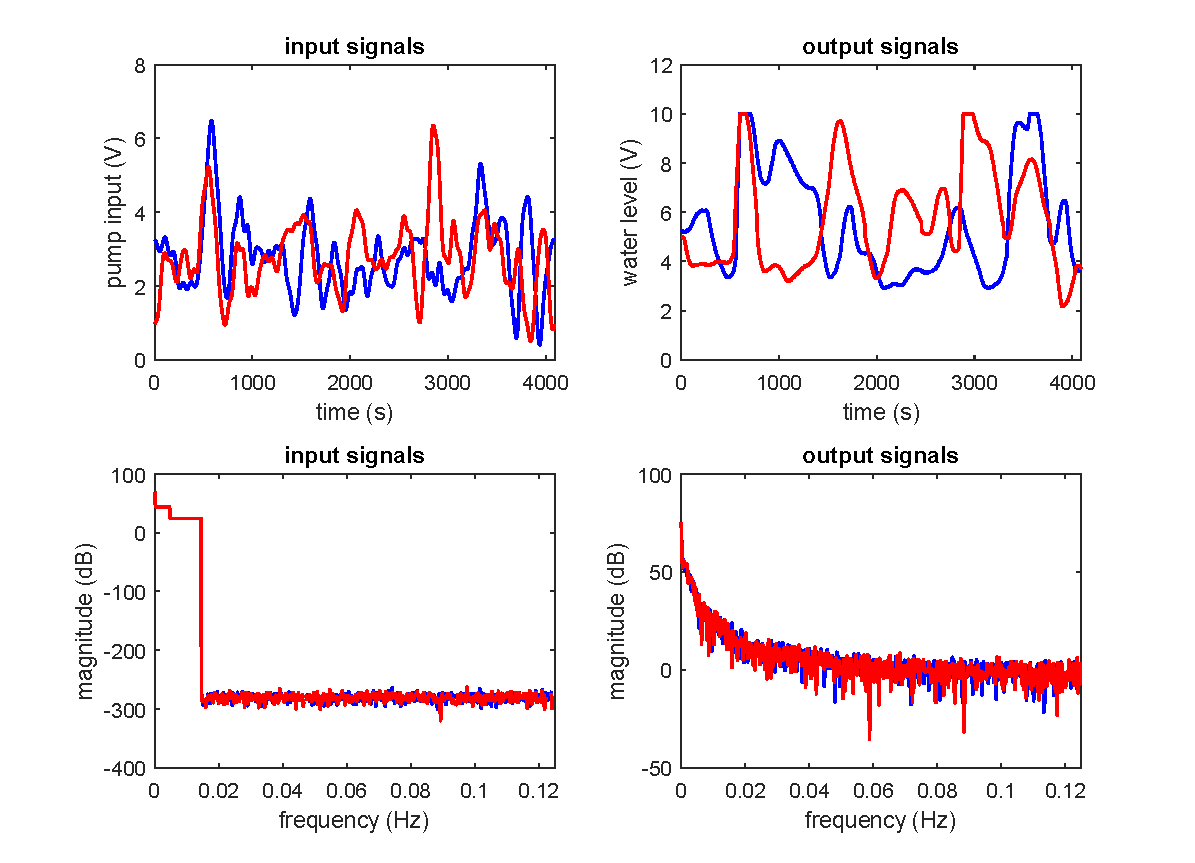
\includegraphics[width=1.05\textwidth]{Chapter6_CaseStudies/Datasets_tanks.pdf}
\caption{Estimation (blue) and validation (red) datasets for the cascaded tanks in the time (top) and frequency (bottom) domain}
\label{fig:datasets_tanks}
\end{figure}

\subsection{Problem statement}

To maintain consistency with the estimates obtained in \cite{Birpoutsoukis2017b}, the identification problem is considered exactly as stated in the benchmark document \cite{Schoukens2016c}. The required outcome is to identify a model of the system using the estimation dataset, and report the accuracy of the estimated model in predicting the output of the \emph{entire} $1024$-sample validation dataset using the following metric, 
\begin{equation}
e_{RMSt} = \sqrt{\frac{1}{N_v} \sum_{t=1}^{N_v} (y_{mod}(t) - y_v(t) )^2},
\label{eq:e_RMSt}
\end{equation}
where $N_v = 1024$ is the length of $y_v$, the validation output, and $y_{mod}$ is the modeled output for the same validation input. Note that prediction of the entire output vector requires estimation of the unknown initial states, since the start of the record will be affected by inputs applied prior to the measurement window. 

\subsection{Estimating unknown initial states}

In the nonparametric Volterra series context, the initial states problem becomes an issue of `past inputs', since Volterra kernel outputs are functions of lagged inputs only. Hence, in order to estimate/validate using the entire output vector, $\{y(t)\}_{t=1}^{1024}$, we require knowledge of $u(t)$ for $n<t<0$ and some reasonable memory length $n$. Of course, no knowledge of these past inputs can be gained from the provided datasets, so two strategies are discussed in this section in order to continue estimating/validating with the complete output vector. Both strategies are applied to the benchmark data in Section \ref{sec:Results_tanks}.

\subsubsection{Bayesian transient estimation}
\label{sec:BayesTrans_tanks}

For consistency, one approach we consider is the method used in \cite{Birpoutsoukis2017b}, whose results will be the subject of comparison for this benchmark. In the paper, which relies on previous results established in \cite{Csurcsia2015}, the input is assumed to be periodic, i.e. $u(t-N) = u(t) \; \forall t$, where $N=1024$ for the cascaded tanks. However, since the system is not in steady state, this assumption is clearly in error, and we expect to see a `transient' function which describes the difference between the measured output and the ideal steady-state output. This difference will be denoted $\theta_{tr}$, which has length $n_{tr}<N$.

In this case, the regression structure for basis function kernels in (\ref{eq:RegressionStructure_OBFseries}) can be updated to include the transient,
\begin{equation}
Y = \Phi_f^T \alpha + \Phi_{\delta} \theta_{tr} + E,
\end{equation}
where the $Y$ vector now contains all $N$ samples of $y(t)$, $\Phi_f$ contains measured \emph{and} unmeasured input values, and $\Phi_{\delta}$ is a $N \times n_{tr}$ rectangular identity. Staying within the Bayesian framework, a Gaussian assumption is placed on $\theta_{tr}$, such that the regularization problem can be augmented as follows,
\begin{align}
&\alpha' = [\alpha^T \; \; \theta_{tr}^T]^T, \; \; \Phi' = [\Phi_f^T \; \; \Phi_{\delta}], \nonumber \\
&\hat{\alpha}'_{ReLS} = \text{arg } \underset{\alpha'}{\text{min}} \|Y - \Phi' \alpha' \|^2_2 + \sigma^2 \alpha'^T [P']^{-1} \alpha',
\end{align}
where $P'$ is an augmented prior covariance matrix given by
$$P' = \begin{bmatrix}
       P &  \mathbf{0} \\
        \mathbf{0}  & P_{tr}
     \end{bmatrix},$$
and $P_{tr}$ is the covariance of $\theta_{tr}$, which is chosen to have the linear DC structure given in (\ref{eq:DCstructure}). The prior covariance, $P$, for the original parameter vector, $\alpha$, is also chosen to be DC-based and is constructed as in previous chapters using (\ref{KernelPenalty}), (\ref{DCext}), and (\ref{FinalPenalty}).

The hyperparameter set, $\eta$ (which now includes hyperparameters for $P_{tr}$) is still tuned with EM using Algorithm \ref{alg:BFopt}, however some minor modifications are made to include the augmented transient components. The $P_{tr}$ hyperparameters are then re-used in the validation dataset, to re-estimate and remove the transient function from the output.

\begin{rem}
\label{rem:BayesTrans}
It is important to note that while the Bayesian transient method is included to be consistent with \cite{Birpoutsoukis2017b}, its requirement to re-estimate the validation transient is not in the spirit of the benchmark problem. Instead, it would be fairer to keep the validation data only for validation purposes, and not for the estimation of any parameters.
\end{rem}

\subsubsection{Constant past input assumption}
\label{sec:ConstInput_tanks}

Observing Remark \ref{rem:BayesTrans}, another approach can be formulated which adds less complexity to the EM optimization, and requires no re-estimation on the validation data. In this approach, we restrict the unmeasured input, $\{u(t)\}_{t=-\infty}^{-1}$ to the class of constant sequences, i.e.
$$u(t) = c \; \; \forall t<0; \; c \in \mathbb{R}^+.$$ 
The constant, $c$, is tuned during the optimization in Algorithm \ref{alg:BFopt} such that the following condition is satisfied in each iteration, 
$$y_P^{(k)}(0) = y(0),$$ 
where $y_P^{(k)}(0)$ is the output value predicted using $\hat{\alpha}^{(k)}$ and past inputs $u(t)=c$ for $t<0$ in the regressor, $\Phi_f$.  

\subsection{Identification results}
\label{sec:Results_tanks}

The regularized estimation method from Chapter \ref{chap:5} (ReLBF) is applied for several orders of the model structure in (\ref{OBFvolterra}) expanded using Laguerre basis functions:
\begin{itemize}
\item A linear LBF expansion, i.e. excluding $\alpha_0$ and setting $M=1$
\item A 2nd order Volterra-Laguerre series (M=2)
\item A 3rd order Volterra-Laguerre series (M=3)
\end{itemize}

The truncation lengths at each order are chosen as $\mathcal{B}_1 = 15$, $\mathcal{B}_2 = 10$ and $\mathcal{B}_3$ = 8, having been obtained through a typical iterative identification process. For the Bayesian transient removal method \cite{Birpoutsoukis2017b}, the length of the transient is defined as $n_{tr} = 100$.

Hyperparameter optimization is achieved using the MATLAB $\text{\tt{GlobalSearch}}$ and $\text{\tt{fmincon}}$ functions to perform all non-convex minimizations in Algorithm \ref{alg:BFopt}. Computation times for the estimation are measured on an Intel Xeon 3.50 GHz processor.

The two methods for dealing with unknown initial states are denoted `Bayesian transient' for the first method in Section \ref{sec:BayesTrans_tanks} and `Constant input' for the second method.

\subsubsection{Estimation and validation}

Modeling the system first with a linear LBF expansion, a reasonable result is achieved, but the shortcomings of a linear model are clear. The estimated LBF coefficients are plotted in Figure \ref{fig:LinearTankEst}, along with the corresponding time-domain impulse response. The choice of $\mathcal{B}_1=15$ is supported by the estimate, and the decay time of the impulse response suggests that $n_{tr}=100$ is a reasonable choice, since the transient function typically decays at the same rate as the system response, at least for linear systems \cite{Lataire2016}.

\begin{figure}[h]
\centering
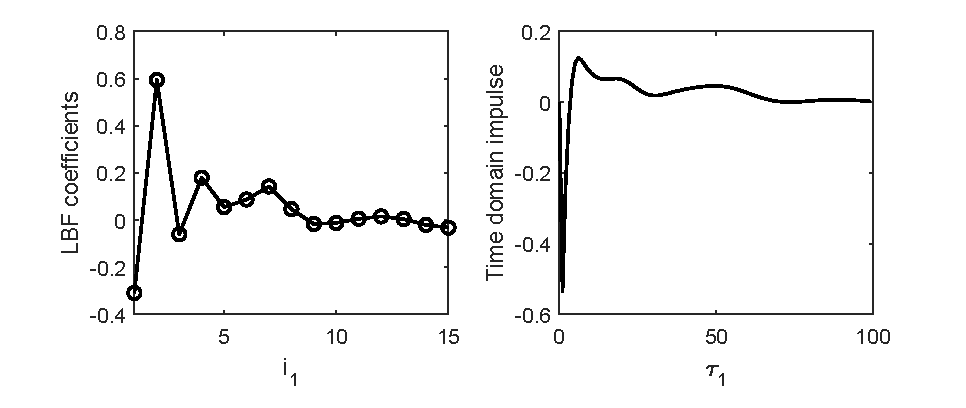
\includegraphics[width=0.9\textwidth]{Chapter6_CaseStudies/LinearLBFs.pdf}
\caption{Linear model for the cascaded tanks: estimated LBF coefficients (left) and equivalent time domain FIR (right)}
\label{fig:LinearTankEst}
\end{figure}

\begin{figure}[h]
\centering
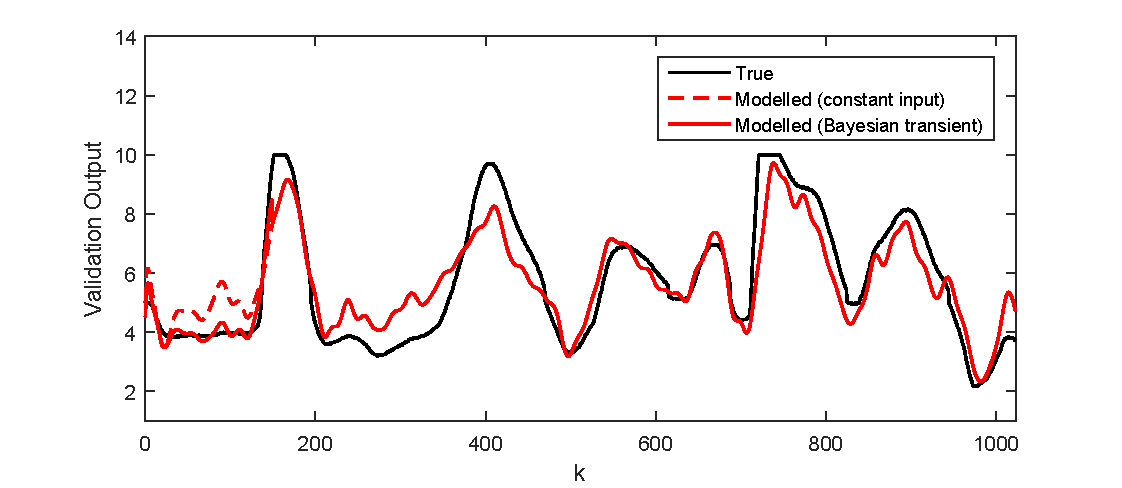
\includegraphics[width=0.9\textwidth]{Chapter6_CaseStudies/LinearValidation.pdf}
\caption{Linear model for the cascaded tanks: true (black) and modeled (red) validation outputs using both transient removal methods}
\label{fig:LinearTankVal}
\end{figure}

The true and modeled validation outputs for the linear estimate are given in Figure \ref{fig:LinearTankVal}, where we see that the modeled output is quite poor in the first half of the record. The Bayesian transient approach is also seen to produce a better result than the constant input assumption, although it relies on some estimation using the validation data. Overall, there is clearly room for improvement, which can likely be achieved by estimating higher order terms of the Volterra-Laguerre series.

Estimating a second order Volterra-Laguerre model, the validation performance is significantly improved. The constant kernel is estimated as $\hat{\alpha}_0 = -4.55$, and the first and second order basis function kernels are plotted in Figure \ref{fig:2ndOrderTankEst}. The true and modeled validation outputs are given in Figure \ref{fig:2ndOrderTankVal}, where it can be observed that the output predicted by the model is visibly more accurate than in the linear case. Furthermore, the Bayesian transient and constant input methods both obtain a good prediction of the initial 100 output samples. 

\begin{figure}[h]
\centering
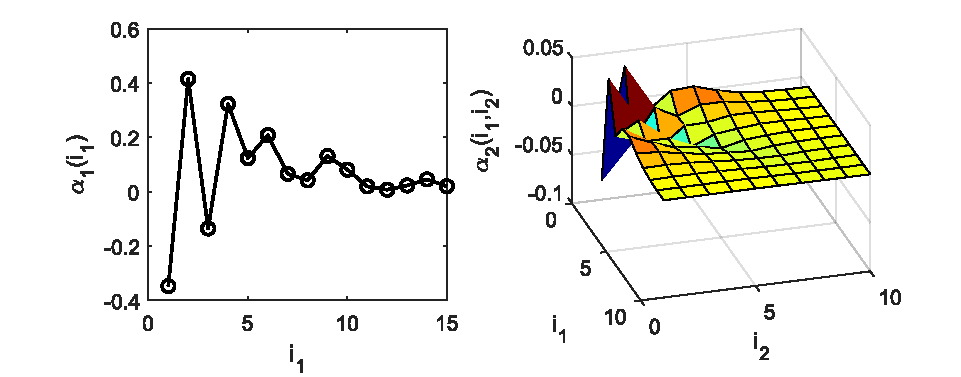
\includegraphics[width=0.9\textwidth]{Chapter6_CaseStudies/Kernels2ndOrder_CT_Coloured.pdf}
\caption{Volterra model (M=2) for the cascaded tanks: estimated 1st order (left) and 2nd order (right) LBF kernels}
\label{fig:2ndOrderTankEst}
\end{figure}

\begin{figure}[h]
\centering
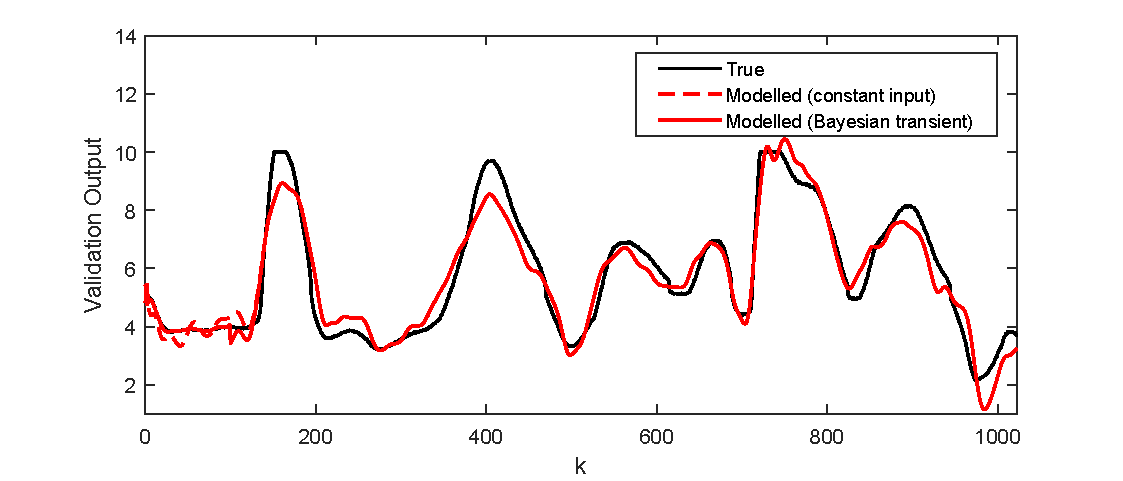
\includegraphics[width=0.9\textwidth]{Chapter6_CaseStudies/2ndOrderValidation.pdf}
\caption{Volterra model (M=2) for the cascaded tanks: true (black) and modeled (red) validation outputs using both transient removal methods}
\label{fig:2ndOrderTankVal}
\end{figure}

The third order Volterra-Laguerre model has aso been estimated, however the improvement in validation performance is negligible with respect to the second order model. The error metrics and computation times are still reported.

The RMS error in the validation is computed for each model and method using (\ref{eq:e_RMSt}), and these errors are compared, in Table \ref{tab:eRMS_tanks}, with the time domain results reported in \cite{Birpoutsoukis2017b}. The results show very similar validation performance between the time domain and LBF approach. The constant input method of transient removal is seen to provide essentially the same accuracy as the Bayesian method (with the exception of the linear case), despite its more simple nature. 

\renewcommand{\arraystretch}{1.3}
\begin{table}[h]
\centering
\caption{Comparison of validation errors between methods}
\label{tab:eRMS_tanks}
\begin{tabular}{|l||r|r|r|}
\hline
                & \multicolumn{3}{c|}{\textbf{$\mathbf{e_{RMSt}}$ (from (\ref{eq:e_RMSt}))}} \\ \cline{2-4} 
\textbf{Model} & Birpoutsoukis           & ReLBF            & ReLBF                \\ 
		&  et. al. (2017) \cite{Birpoutsoukis2017b}          & (Bayesian)           & (Constant)                \\ \hline 
Linear         & 0.84              & 0.85             & 0.91                            \\ \hline
Volterra (M=2)         & 0.55               & 0.56             & 0.57                             \\ \hline
Volterra (M=3)           & 0.54              & 0.56             & 0.56                             \\ \hline
\end{tabular}
\end{table}

While the validation performance of the time domain and basis function Volterra models is extremely similar for the cascaded tanks benchmark, significant advantages of the basis function formulation can be seen when comparing the numbers of unique parameters required, and the computation time required for model estimation. In Table \ref{tab:Params+Times_tanks}, the total parameter numbers and computation times are reported for the LBF method, alongside the corresponding figures for the time domain approach as reported in \cite{Birpoutsoukis2017c}. It is clear that a LBF formulation of the regularized problem produces far more compact Volterra models, with an order of magnitude difference in the parameter numbers. As a direct consequence, the difference in computation time is even greater, where the Volterra-Laguerre estimates are computed two or three orders of magnitude faster.

\renewcommand{\arraystretch}{1.3}
\begin{table}[h]
\centering
\caption{Comparison of computation time and parameter numbers between methods}
\label{tab:Params+Times_tanks}
\begin{tabular}{|l||c|c||c|c|}
\hline
                & \multicolumn{2}{c||}{\textbf{Parameters}} & \multicolumn{2}{c|}{\textbf{Comp. Time (mins)}}  \\ \cline{2-5} 
\textbf{Model} & Time domain         & ReLBF            &Time domain           & ReLBF                \\ \hline
Linear                   & 92                     & 15    &   3          &  0.1 \\ \hline
Volterra (M=2)                 & 721      &  71        & 210             &  0.6                \\ \hline
Volterra (M=3)                     & 860      & 191      & 390             &  2                 \\ \hline
\end{tabular}
\end{table}

%---------------------------------------------------------------------------------------------------------------------------------------------------------------------------------------------------------------------------------------

\section{Coupled electric drives}

The coupled electric drives is a benchmark system inspired by an example which appeared in \cite{Wellstead1979}. The original example was designed to represent machines which transfer a belt of material from one spool to another using two electric drives and a pulley. In the benchmark problem, a data set of only 500 samples is provided for estimation purposes. The system has previously been modeled using block-oriented models, where the structure is derived from knowledge of the relevant physical interactions \cite{Wigren2017}. As was done for the cascaded tanks benchmark, here the identification problem will be approached from a position of no prior knowledge, to highlight the versatility of Volterra series modeling even when using an extremely short estimation dataset. The comparison for the drives system will be between regularized basis function estimates (using ReLBF) and estimates obtained using several other popular nonlinear model classes. 

\subsection{System description}
\label{sec:CED_description}

The benchmark system is configured as shown in Figure \ref{fig:CoupledDrivesSchematic}, where the input is simultaneously applied to two motors driving a flexible belt, which in turn rotates a pulley being held by a spring. The angular speed of the pulley is measured by a pulse transducer, whose measurement is sent through an analogue low-pass and anti-aliasing filter to produce the final speed output which can be used for control purposes.  

\begin{figure}[h]
\centering
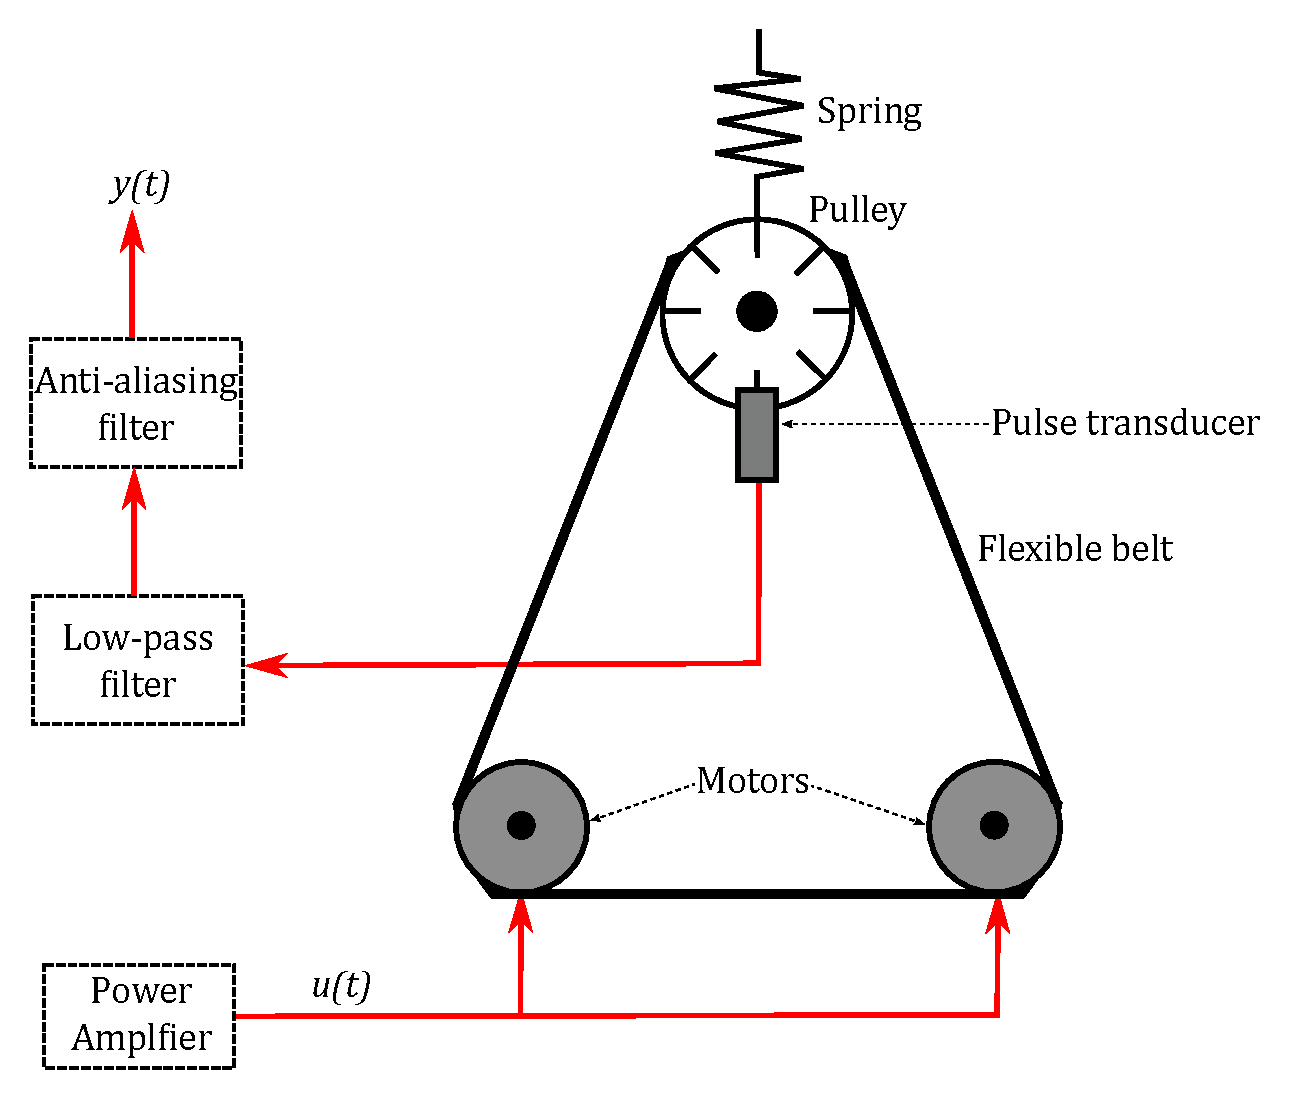
\includegraphics[width=0.75\textwidth]{Chapter6_CaseStudies/DrivesSchematic.pdf}
\caption{Schematic of the coupled electric drives benchmark system} \label{fig:CoupledDrivesSchematic}
\end{figure}

The spring and flexible belt add lightly damped dynamic modes to the system, and there will also be time constants associated with the motors, however these are all linear effects. The modeling complication is brought about by the pulse transducer, which is insensitive to the \emph{direction} of rotation of the pulley, since it simply counts pulses to approximate angular velocity. As the motors can be driven in either direction, the transducer can be considered as having an `absolute value' nonlinearity, such that the total system is well approximated by a Wiener-Hammerstein block structure, as depicted in Figure \ref{fig:WienerHamm_CED}. 

\begin{figure}[h]
\centering
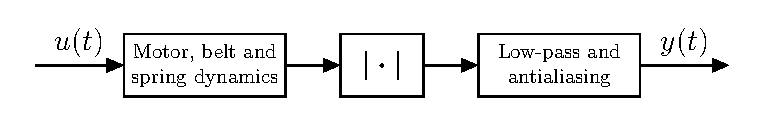
\includegraphics[scale = 1]{Chapter6_CaseStudies/WienerHammCED.pdf}
\caption{Wiener-Hammerstein block structure for the coupled electric drives} \label{fig:WienerHamm_CED}
\end{figure}

\subsection{Measurement process}

While some physical modeling insights can be obtained by analyzing the system set-up, it is the experimental input-output data which will be used to identify and assess candidate models. An estimation and a validation dataset have been recorded, both containing 500 input-output samples recorded at 50 Hz. The inputs are constructed from a Pseudo-Random Binary Sequence (PRBS) which is multiplied by a noise sequence with uniform distribution. The input and output signals for each set are shown in Figure \ref{fig:EstimationData_CED}. The validation input is seen to be the estimation input shifted by an offset of +0.5V, and the absolute value nonlinearity is clearly visible in the output signals.

\begin{figure}[h]
\centering
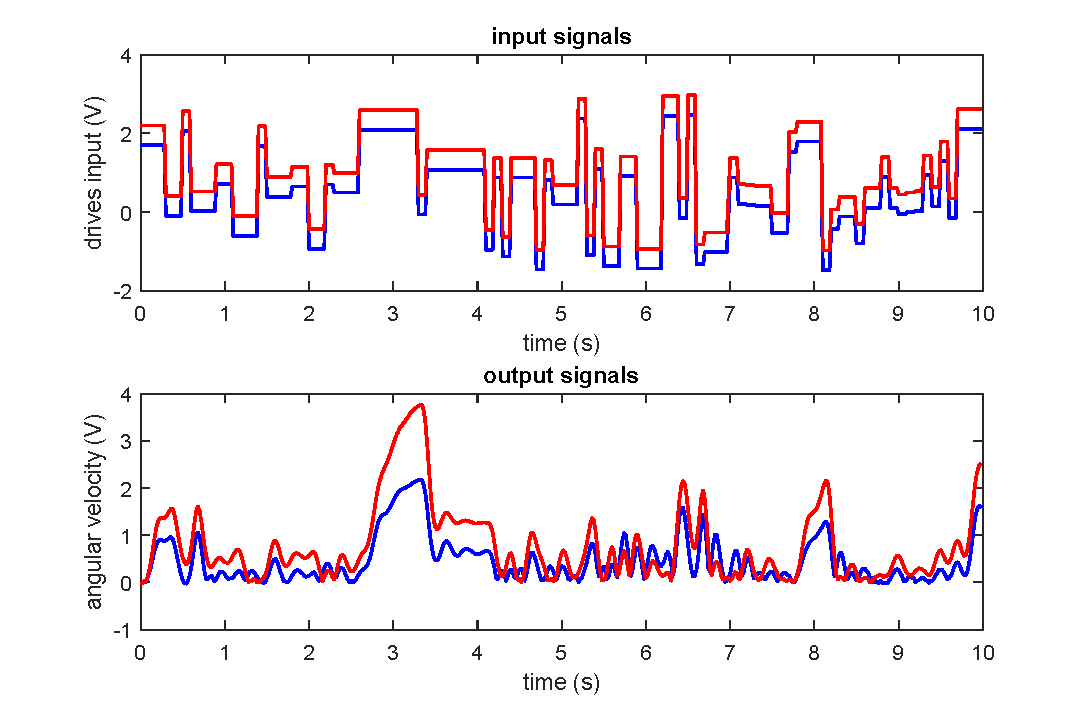
\includegraphics[width=0.95\textwidth]{Chapter6_CaseStudies/Datasets_drives.pdf}
\caption{Input (top) and output (bottom) signals for the coupled electric drives estimation (blue) and validation (red) datasets} \label{fig:EstimationData_CED}
\end{figure}

\subsection{Problem statement}

The identification problem for the coupled electric drives is to estimate a nonlinear model using the estimation data, and use this model to predict the output for the validation dataset. Unlike the cascaded tanks benchmark, the issue of estimating initial states will not be considered. Instead, the model predicted output begins at the 60\textsuperscript{th} sample, when enough measured input information is available.

The performance of each nonlinear model on the validation data is assessed numerically, using a normalized root mean square error (NRMSE) metric defined by 
\begin{equation}
\text{NRMSE} = 1 - \frac{||Y_{val}-Y_{mod}||_2}{||Y_{val} - \text{mean}(Y_{val}) ||_2},
\label{eqn:NRMSE_CED}
\end{equation}
where $Y_{val}$ is the true validation output vector and $Y_{mod}$ is the model-predicted output vector.

\subsection{Identification results}
\label{sec:Results_CED}

LBF-expanded Volterra kernels are estimated for the benchmark system using the ReLBF method proposed in Chapter \ref{chap:5}. Due to the limited number of estimation samples available, the order of the Volterra series is fixed at $M=2$, and using no prior knowledge of the system, the number of basis functions for each order is chosen to be $\mathcal{B}_1=\mathcal{B}_2=20$, such that the total number of unique parameters requiring estimation (231) is roughly half the number of data samples available. All non-convex optimization problems in Algorithm \ref{alg:BFopt} are solved using the MATLAB $\text{\tt{GlobalSearch}}$ and $\text{\tt{fmincon}}$ functions to locate a global minimum.

\begin{figure}[!b]
\centering
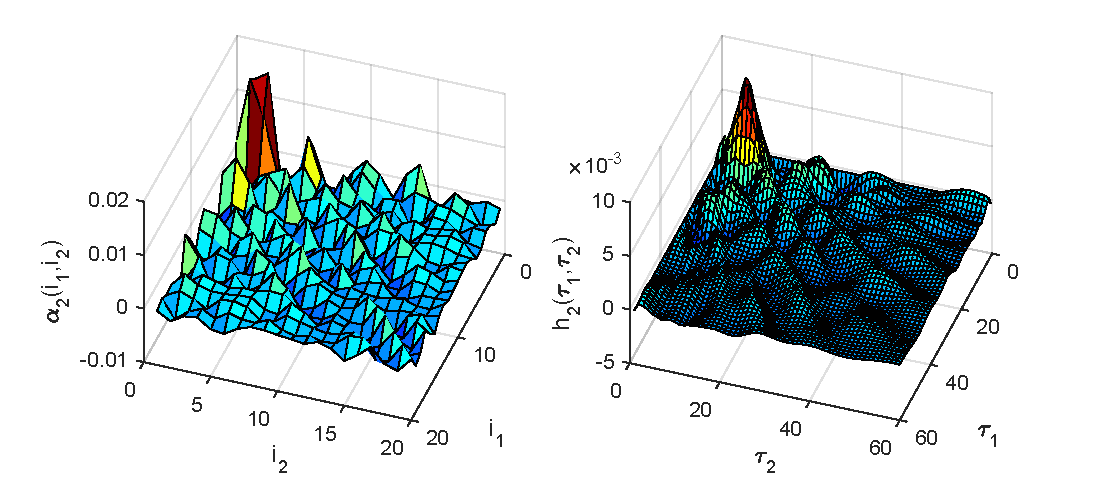
\includegraphics[width=\textwidth]{Chapter6_CaseStudies/Kernels2ndOrder_CED_Coloured}
\caption{Estimated 2\textsuperscript{nd} order LBF kernel (left) and its time domain equivalent (right) for the coupled electric drives} \label{fig:Kernel2_CED}
\end{figure}

The first order kernel, $\hat{\alpha}_1$, is estimated to be negligible. This is to be expected, since the absolute value nonlinearity is an \emph{even} function and as such generates only even order Volterra kernels in the series expansion. The second order LBF kernel estimate, $\hat{\alpha}_2$, is shown in Figure \ref{fig:Kernel2_CED} as well as its time domain equivalent, $\hat{h}_2$. The zeroth order kernel is estimated as $\hat{\alpha}_0 = 0.102$.

Applying the validation input to the estimated Volterra-Laguerre model produces the output prediction shown in Figure \ref{fig:ValidationLBFVK_CED}, which is plotted with the given validation output. Despite using only 500 samples for estimation, the regularized basis function approach provides a very accurate model which is suitable for prediction or control purposes. 

\begin{figure}[h]
\centering
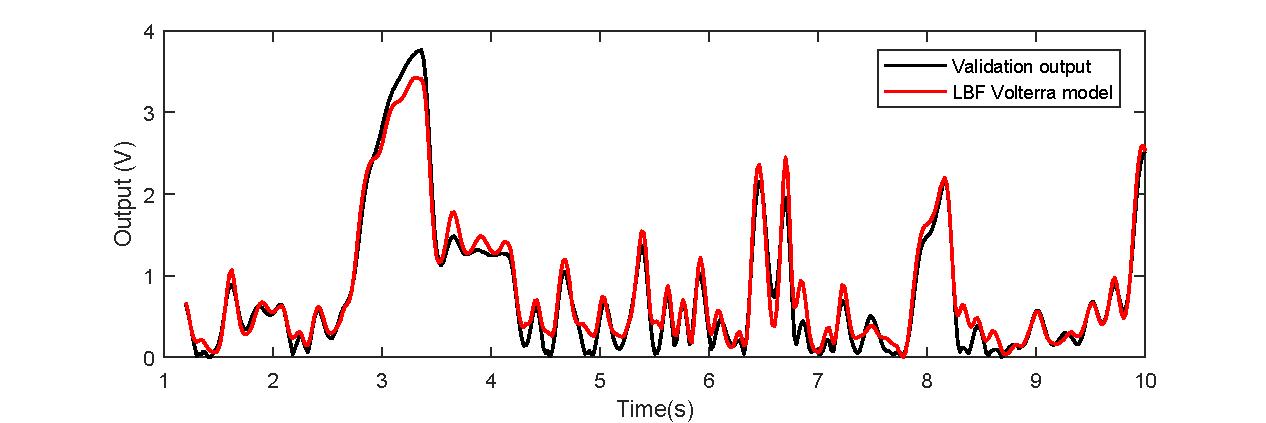
\includegraphics[width=\textwidth]{Chapter6_CaseStudies/ValidationLBFVK_CED.pdf}
\caption{True and model-predicted validation outputs for the Volterra-Laguerre model applied to the coupled electric drives benchmark} \label{fig:ValidationLBFVK_CED}
\end{figure}

\subsubsection{Comparison with Alternate Methods }

In order to provide some context when assessing the performance of the proposed method, several alternate model classes and methods are also applied to the coupled electric drives benchmark. The other models considered are:
\begin{enumerate}
\item Linear state space 
\item Linear transfer function 
\item Nonlinear ARX (NARX) 
\item Wiener block structure
\end{enumerate}

For each model class, the estimation dataset is used to estimate a model using the appropriate method provided by MATLAB's System Identification toolbox. As in the proposed ReLBF method, no prior knowledge is used in the estimation, and the model orders for each case are chosen based on a cross-validation approach. High order polynomials are used for nonlinear function estimates. Note that Wiener-Hammerstein models cannot be estimated using the toolbox, however this case has already been treated in~\cite{Wigren2017}.

The predicted validation output from each model is plotted in Figure \ref{fig:ValidationToolbox_CED}, along with the true experimental output (in black). It is clear that for such a short estimation dataset, and without the use of prior knowledge, none of the estimated models provide accurate predictions over the entire validation set for the coupled electric drives system. 

\begin{figure}[h]
\centering
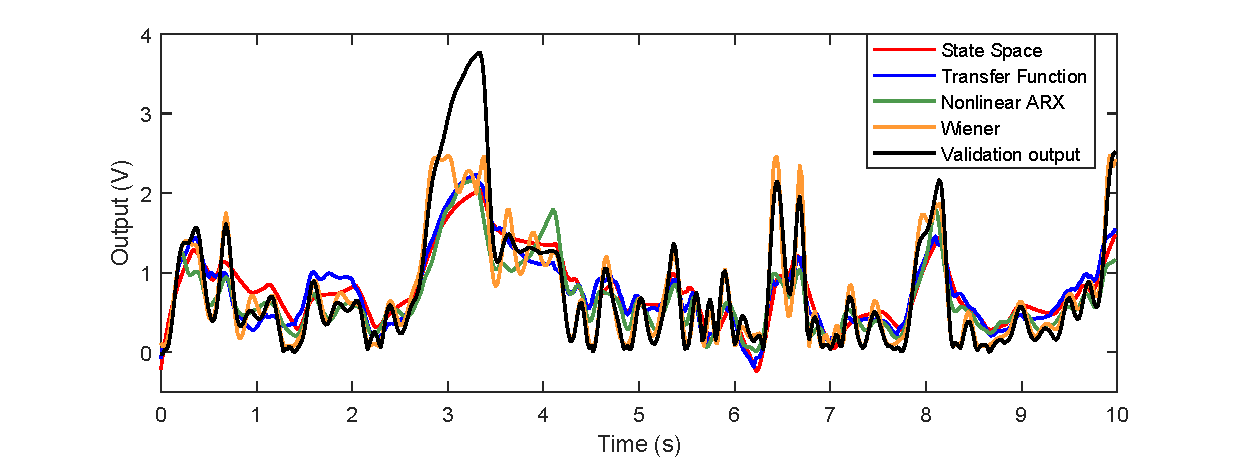
\includegraphics[width=\textwidth]{Chapter6_CaseStudies/ToolboxValidations_CED.pdf}
\caption{True and model-predicted validation outputs for toolbox methods in MATLAB applied to the coupled electric drives benchmark} \label{fig:ValidationToolbox_CED}
\end{figure}

The NRMSE error metric (\ref{eqn:NRMSE_CED}) for each toolbox method is compared in Table \ref{tab:NRMSE_CED} against the method proposed in this thesis (ReLBF), highlighting the superior performance of the regularized nonparametric approach. From the four toolbox models, the Wiener structure produces the next best validation results, which can be attributed to the Wiener-Hammerstein nature of the true system (see Figure \ref{fig:WienerHamm_CED}), where the final linear filter block contains dynamics which could be considered negligible. This is further supported by the fact that similar prediction performance was achieved using a Wiener-Hammerstein model in \cite{Wigren2017}.

\begin{table}[h]
\centering
\caption{NRMSE in validation for proposed and toolbox methods}\label{tab:NRMSE_CED}
\begin{tabular}{|c||c|c|c|c|c|}
\hline
\textbf{Model} & State Space & Transfer Func. & NARX & Wiener &\emph{ReLBF} \\
\hline
\textbf{NRMSE} & 0.402 & 0.457 & 0.446 & 0.639 & 0.811 \\
\hline
\end{tabular}
\end{table}

\section{Conclusion}

The Volterra series has historically been regarded as an impractical tool for data-driven modeling. The benchmark examples in this chapter, however, have shown that by using a more compact basis function formulation, and efficiently regularizing the estimation to impose known properties of smoothness and decay, the Volterra series \emph{can} be a broad and powerful tool for nonlinear system identification. 

The cascaded tanks benchmark revealed that a regularized basis function method can be adapted to deal with unknown initial states in a system. The resulting 2\textsuperscript{nd} and 3\textsuperscript{rd} order series estimates gave reasonably accurate prediction performance, despite the short data record used for estimation. This performance was compared against the time domain estimation method in \cite{Birpoutsoukis2017b}, showing equivalent validation metrics but a stark decrease in parameter numbers and computation times for the proposed basis function approach. 

The coupled electric drives benchmark provided further evidence for the proposed method. Despite having an even shorter estimation dataset of 500 samples, and without incorporating prior knowledge of the drives system into the modeling process, the estimated Volterra-Laguerre kernels provided accurate predictions in the validation step. Furthermore, the proposed method significantly outperformed linear and nonlinear models provided by the established System Identification toolbox in MATLAB in terms of the considered error metric.

%--------------------------------------------------------------------------------------------------------------------------------------------------
\cleardoublepage
\part{Frequency Domain Identification}
\label{part:FD}
%--------------------------------------------------------------------------------------------------------------------------------------------------

\cleardoublepage
\chapter{Gaussian Process Regression in the Frequency Domain - the Parallel Hammerstein Case}
\label{chap:7}
\emph{Frequency domain estimation of parallel Hammerstein systems is considered in this chapter, using nonlinear output frequency response functions (NOFRFs). The NOFRFs are a series of one-dimensional frequency functions which are input dependent in general, however, they can be shown to be input independent linear filters in the parallel Hammerstein case. A Gaussian process regression (GPR) framework is proposed for the NOFRF estimation, using concepts adapted from the linear identification literature. When compared to the existing multi-level excitation method, the proposed GPR approach is less sensitive to noisy measurements and requires fewer experimental restrictions.}
\newpage
\section{Introduction}

In Chapter \ref{sec:DTrepresentations_Volterra}, several competing representations were discussed for Volterra series modeling in the frequency domain, where each representation offers different benefits for interpretation and estimation \citep{Rijlaarsdam2017}, \citep{Cheng2017}. The GFRFs give perhaps the most natural representation, being multidimensional Fourier transforms of their corresponding time domain Volterra kernels ~\citep{George1959}. However, due to the complex multidimensional nature of the GFRFs, the NOFRF model was proposed \cite{Lang2005} to increase the ease of system analysis.  The model (see (\ref{eq:NOFRF_TransientFree})) contains only one-dimensional frequency functions which have a more intuitive interpretation from the perspective of linear systems theory, however, the functions are input dependent in general. This input dependence has restricted the use of NOFRFs to cases where input behaviour remains uniform over time, such as fault detection applications \citep{Peng2007}, \citep{Cao2013}, \citep{Xia2015} and nonlinearity detection \citep{Lang2008}. 

The NOFRF model proposal  in \cite{Lang2005} was accompanied by a data-driven identification algorithm, which uses multi-level excitation to estimate NOFRFs in a regression framework. This traditional method requires multiple experiments on the system under conditions that may not be possible in practice if the system excitation cannot be precisely controlled. The method also employs a least squares estimator that is sensitive to noisy measurements. In the special case of parallel Hammerstein systems it is possible to perform more sophisticated estimation, since the NOFRFs become independent of the applied input and the form of the functions closely resemble that of the underlying linear filters in the system's block structure. This property allows us to adopt well-developed concepts from linear identification theory.

The Bayesian regularization method for FIR estimation \cite{Pillonetto2010}, which provided the framework for contributions in Part \ref{part:TD} of this thesis, also has a linear frequency domain interpretation. Developed in \cite{Lataire2016}, the frequency domain method considers estimation of FRFs via Gaussian process regression (GPR). However, some additional challenges arise in the frequency domain case, due to the emergence of a transient function in the output spectrum when using non-steady-state data and the mixture of real and complex parameters contained in the FRF parameter vector. The results in \cite{Lataire2016} will provide a foundation for many of the contributions contained in Part \ref{part:FD} of the thesis. 

In this chapter, a GPR method is developed for estimating NOFRFs in the special case of a parallel Hammerstein system. The method is an extension to the linear frequency domain method in \cite{Lataire2016}. By framing the NOFRFs as normally distributed quantities with standard prior covariance structures, we can estimate all NOFRFs in a regularized fashion using only one experiment and with less restrictions than the traditional multi-level excitation method. Numerical examples reveal that the method proposed here is also significantly less sensitive to measurement noise than the traditional method in \cite{Lang2005}. The general case of non-steady-state data is also considered, where the GPR approach can be adapted to minimize the effect of transients on NOFRF estimation. 

The proposed method is distinct from other parallel Hammerstein identification algorithms in that it is a fully nonparametric method applied directly in the frequency domain. Traditionally, the linear dynamic and nonlinear blocks are estimated separately, and parametrically, in an iterative scheme \cite{Gallman1975}, \cite{Schoukens2011}, however the resulting models do not provide direct intuition on frequency domain behaviour. More recently, GPR has been applied to Hammerstein identification in the time domain~\cite{Risuleo2017}, but the approach was limited to a single Hammerstein branch.

\section{Real/complex normal distributions}
\label{sec:RCN}

The parameter vectors considered in the current chapter, as well as Chapter \ref{chap:8}, are free to contain both real and complex parameters. In order to express the distribution of Gaussian random vectors that contain both real and complex entries, the complex normal distribution \cite{Schreier2010} is not sufficient, since the associated augmented covariance matrix will be singular. Consequently, a hybrid Real/Complex Gaussian (RCG) distribution framework was developed in \cite{Lataire2016}, which will also be used in the sequel for parameter estimation. In this section we define some relevant notation and properties to enhance the readability of Chapters \ref{chap:7} and \ref{chap:8}. 

\begin{defn}[Real/Complex Gaussian vector]
A random vector
\begin{equation}
\label{eqn:RCG_vector_defn}
X = \begin{bmatrix} {X^{\mathbb{R}}} \\ {X^{\mathbb{C}}} \end{bmatrix}, \; \; \; X^{\mathbb{R}} \in \mathbb{R}^{n_r}, \; X^{\mathbb{C}} \in \mathbb{C}^{n_c}
\end{equation}
is said to be a RCG vector if the vector $$\begin{bmatrix} {X^{\mathbb{R}}} \\ \mathfrak{R}{X^{\mathbb{C}}} \\ \mathfrak{I}{X^{\mathbb{C}}} \end{bmatrix}$$ is Gaussian distributed, where $\mathfrak{R}$ and $\mathfrak{I}$ give the real and imaginary parts respectively. 
\end{defn}

\begin{notation}[Augmented vector]
For a RCG vector, $X$, the augmented vector is defined as 
\begin{equation}
\widetilde{X} = \begin{bmatrix} {X^{\mathbb{R}}} \\ {X^{\mathbb{C}}} \\ \bar{X}^{\mathbb{C}} \end{bmatrix}, 
\label{eq:augvector_defn}
\end{equation}
where $\bar{X}$ denotes the complex conjugate of a vector $X$.
\end{notation}

\begin{notation}[Augmented mean and covariance]
A RCG vector $X$ has a real/complex normal distribution denoted by
\begin{equation}
X \sim \mathcal{RCN}(\mu,\Sigma),
\label{eq:RCNdistribution_defn}
\end{equation}
where $\mu = \textbf{E}\{\widetilde{X}\}$ is the augmented mean, $\Sigma = \textbf{E} \{ (\widetilde{X} - \mu)(\widetilde{X}-\mu)^H \}$ is the augmented covariance, and $H$ is the Hermitian transpose operator. The augmented covariance, $\Sigma$, can be decomposed using covariance functions $R$, $Q$, $K$, and relation function $C$, as
\begin{align}
&\Sigma = \begin{bmatrix}  R & Q & \overline{Q} \\ Q^H & K & C \\ \overline{Q^H} & C^H & \overline{K}\end{bmatrix} \label{eqn:augmented_covariance} \\ \nonumber \\
\text{where } 	R &= \textbf{E}\{(X^{\mathbb{R}} - \textbf{E}\{{X^{\mathbb{R}}}\})(X^{\mathbb{R}} - \textbf{E}\{{X^{\mathbb{R}}}\})^T\}, \nonumber \\ 
			Q &= \textbf{E}\{(X^{\mathbb{R}} - \textbf{E}\{{X^{\mathbb{R}}}\})(X^{\mathbb{C}} - \textbf{E}\{{X^{\mathbb{C}}}\})^H\}, \nonumber \\ 
			K &= \textbf{E}\{(X^{\mathbb{C}}- \textbf{E}\{{X^{\mathbb{C}}}\})(X^{\mathbb{C}}- \textbf{E}\{{X^{\mathbb{C}}}\})^H\}, \nonumber \\ 
			C &= \textbf{E}\{(X^{\mathbb{C}} - \textbf{E}\{{X^{\mathbb{C}}}\})(X^{\mathbb{C}} - \textbf{E}\{{X^{\mathbb{C}}}\})^T\}. \nonumber
\end{align}
\end{notation}

For the following properties, consider $A \sim \mathcal{RCN}(\mu_A,\Sigma_A)$ and $B \sim \mathcal{RCN}(\mu_B,\Sigma_B)$

\begin{property}[Independent Sum]
\label{prop:IndSum}
For $A$ and $B$ independent and of equal dimension, their sum is distributed as
\begin{equation}
A+B \sim \mathcal{RCN}(\mu_A + \mu_B,\Sigma_A+\Sigma_B).
\end{equation}
\end{property}

\begin{property}[Hadamard Product]
\label{prop:HadProd}
For a complex vector $U$ with equal dimension to $A$, the Hadamard product $U \circ A$ is distributed as
\begin{equation}
U \circ A \sim \mathcal{RCN}(\widetilde{U} \circ \mu_A,(\widetilde{U} \widetilde{U}^H) \circ \Sigma_A).
\end{equation}
\end{property}

\begin{property}[Conditional Distributions]
\label{prop:CondDist}
If A and B are jointly (Gaussian) distributed, the conditional distribution of $A$ given $B$ is given by
\begin{equation}
A|B \sim \mathcal{RCN}\big(\mu_A + \Sigma_{AB} \Sigma_B^{-1}(\widetilde{B}-\mu_B),\Sigma_A - \Sigma_{AB} \Sigma_B^{-1} \Sigma_{BA} \big),
\end{equation}
where $\Sigma_{AB} = \textbf{E} \{ (\widetilde{A}-\mu_A)(\widetilde{B}-\mu_B) \}$. 
\end{property}

\section{The NOFRF model}

Some relevant concepts relating to the NOFRF model structure will be reviewed and clarified here. First, let $u(t)$ and $y_0(t)$ be discrete, noiseless input and output measurements respectively from a nonlinear system, where $t = 0,1,\hdots,N-1$. The $N$-point discrete Fourier transforms (DFTs) of $u$ and $y_0$ will be labelled $U(k)$ and $Y_0(k)$ respectively, where $k \in (0,1,\hdots,N-1)$ indicates the frequency bin. 

The original NOFRF model definition in \cite{Lang2005} assumes that the frequency domain output, $Y_0(k)$, is transient-free. The assumption implies that the input to the system is periodic in $N$ and has been applied for an infinitely long period before measurements were taken, such that the output measurement is one period of a steady-state $N$-periodic signal. In this case, the noise-less output spectrum is given by (\ref{eq:NOFRF_TransientFree}), repeated here for convenience:
\begin{equation}
\begin{split}
Y_0(k) &= H_0(k) + \sum_{m=1}^{M} Y_m(k), \\
Y_m(k) &= G_m(k) U_m(k).  \label{eq:NOFRF_TransientFree_Chap7}
\end{split}
\end{equation}
Recall that $G_m(k)$ is the $m$\textsuperscript{th} order NOFRF, $H_0(k)$ is a zero frequency contribution, and $U_m(k)$ is the DFT of $u^m(t)$. Recall also the equivalent NOFRF block structure, which is repeated here in Figure \ref{fig:NOFRF_ModelStructure_Chap7}, showing the intuitive interpretation of NOFRFs as linear filters on the nonlinear input quantities.

\begin{figure}[h]
\centering
\includegraphics[width=0.9\textwidth]{Chapter7_NOFRFs/NOFRF_blockstructure}
\caption{Equivalent block structure of the NOFRF model}
\label{fig:NOFRF_ModelStructure_Chap7}
\end{figure}

In this chapter, for estimation, the model will also include additive white Gaussian measurement noise at the output. Thus, the \emph{observed} output spectrum is given by
\begin{equation}
\label{eq:NOFRF_Noisy}
Y(k) = Y_0(k) + E(k),
\end{equation} 
where $E(k)$ is assumed i.i.d. with augmented covariance $\sigma^2 I$.

\subsection{The parallel Hammerstein case}

The NOFRFs are input-dependent in general, since they act on exponents of the input rather than the input directly. There exist some special cases in which the frequency functions become independent of the applied input, notably when the system has a parallel Hammerstein structure with polynomial nonlinearities. This structure is depicted in Figure \ref{fig:PolynomialHamm}, where there are $L$ distinct Hammerstein branches, and each branch has a nonlinearity with maximum degree less than or equal to $M$. 

\begin{figure}[h]
\centering
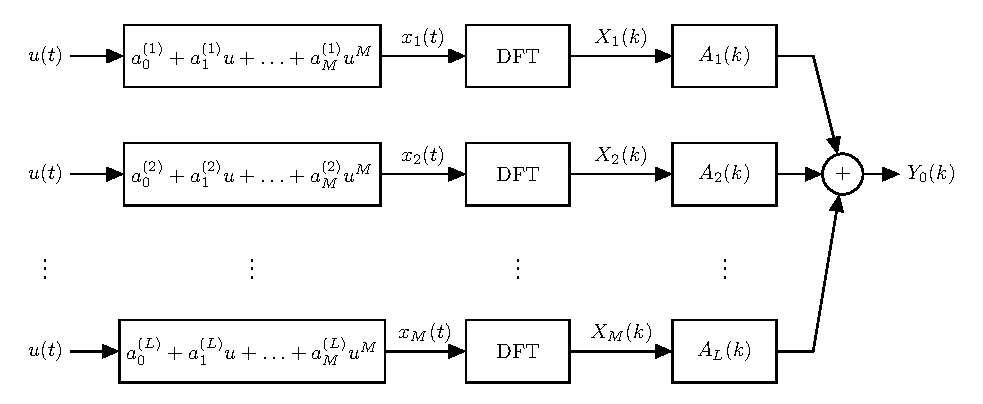
\includegraphics[width=\textwidth]{Chapter7_NOFRFs/ParallelHammStructure}
\caption{Frequency domain block structure of a parallel Hammerstein system with polynomial nonlinearities}
\label{fig:PolynomialHamm}
\end{figure}

To understand why the NOFRFs of such a system are input-independent, the structure can be rearranged by exploiting the linearity of the DFT and the filters, $A_1, A_2, \hdots, A_L$. An alternate parallel Hammerstein block structure is given in Figure \ref{fig:AlternateHamm}, where each exponent of the input is collected in a separate branch, and $H_0(k)$ is a zero frequency contribution produced by the polynomial constants, $a_0^{(i)}, \; \; i = 1,\hdots,L$.  Clearly, this alternate structure matches the NOFRF model structure in Figure \ref{fig:NOFRF_ModelStructure_Chap7}, where the NOFRFs are replaced by 
\begin{equation}
G_m = a_m^{(1)}A_1 + \hdots + a_m^{(L)}A_L \; \; \; m = 1,2,\hdots,M.
\end{equation} 
Thus, for a parallel Hammerstein system, the NOFRFs are linear combinations of the filters from each branch, and since the original filters are all linear and input-independent, the resulting NOFRFs must be also. This is the case which will be considered in the current chapter, where the NOFRFs can be treated as linear filters for identification, and the resulting model will be valid regardless of the system input. 

\begin{figure}[h]
\centering
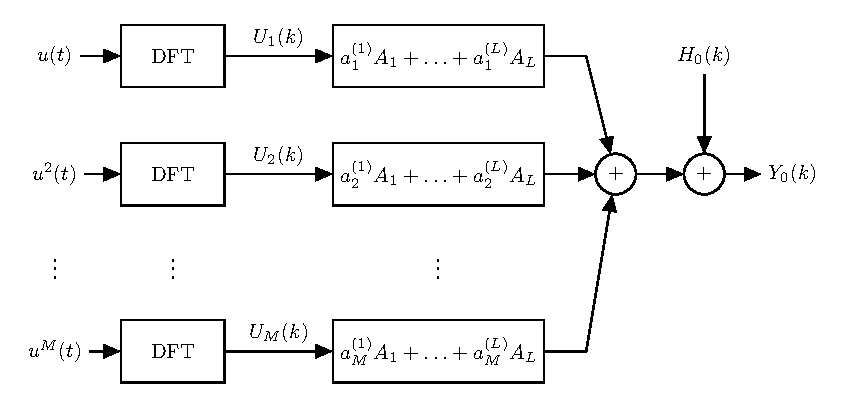
\includegraphics[width=\textwidth]{Chapter7_NOFRFs/AlternateParallelHammStructure}
\caption{Alternate block structure for the parallel Hammerstein system}
\label{fig:AlternateHamm}
\end{figure}

%--------------------------------------------------------------------------------------------------------------------------------------------------------------------------------------------------------

\section{Identification using multi-level excitation}
\label{sec:NOFRFS_multilevel}

The introduction of the NOFRF model in \cite{Lang2005} was accompanied by a data-driven identification scheme. The proposed method requires the system to be excited multiple times by scaled versions of a prototype input signal. Labelling the unscaled prototype input as $u^*(t)$, the set of applied input signals is given by,
$$\beta_i u^*(t), \ \ \ \ i = 1, \hdots, q, \; \; \beta_i \in \mathbb{R}^+,$$
where $q \geq M$ is the total number of excitation levels used. The excitations will produce $q$ corresponding output frequency responses which are denoted as $Y^{(q)}(k)$.

Given the model structure in (\ref{eq:NOFRF_Noisy}), a regression model can be formed at each frequency bin, $k$, using the $q$ excitations applied to the system. These models have the form,
\begin{equation}
\mathbf{Y}(k) = \mathbf{U^*}(k) \mathbf{G}(k) + E,
\label{eq:NOFRF_regressionmodel}
\end{equation}
where
\begin{align}
\mathbf{Y}(k) = \begin{bmatrix} Y^{(1)}(k) \\ \vdots \\ Y^{(q)}(k)\end{bmatrix}, \; \; \mathbf{U^*}(k) = \begin{bmatrix} \beta_1 U^*_1(k) & \hdots & \beta_1^M U^*_M(k) \\ \vdots &\ddots & \vdots \\ \beta_q U^*_1(k) & \hdots & \beta_q^M U^*_M(k) \end{bmatrix}, \; \; \mathbf{G}(k) = \begin{bmatrix} G_1(k) \\ \vdots \\ G_M(k)\end{bmatrix},
\end{align} 
and $U^*_1,\hdots,U^*_M$ are the nonlinear spectral quantities in (\ref{eq:NOFRF_TransientFree_Chap7}) corresponding to $u^*(t)$. 

Least squares estimates for the NOFRFs can be obtained analytically from (\ref{eq:NOFRF_regressionmodel}) at any given frequency. If the error vector $E$ is circular complex distributed, the solution is given as
\begin{equation}
\hat{\mathbf{G}}(k) = \bigg( \big[ \mathbf{U^*}(k) \big]^H \big[ \mathbf{U^*}(k) \big] \bigg)^{-1} \big[ \mathbf{U^*}(k) \big]^H \mathbf{Y}(k) \; \; \; \forall k \in \mathcal{K}
\end{equation}
where $\mathcal{K}$ is the set of excited frequency bins in the input, $U^*_1(k)$. For any other distribution of $E$, (\ref{eq:NOFRF_regressionmodel}) must be separated into its real and imaginary parts, with each part solved separately in the traditional least squares sense (see \cite{Lang2005}).  

This multi-level excitation method for NOFRF estimation has several disadvantages:
\begin{itemize}
\item Data collection may take a long time to perform, requiring at least $M$ experiments which must reach steady-state before measuring.
\item The method cannot be used in cases where the input is not precisely controlled.
\item Least squares solutions are sensitive to measurement noise.
\item The quantity and value of scaling parameters, $\beta_i$, are arbitrary choices which are made by the user.
\end{itemize}
These shortcomings highlight the need for a more sophisticated algorithm, capable of accurate parameter estimation in a generic and noisy experimental setting. In the case of parallel Hammerstein systems, such an algorithm will be developed in the sequel.

%--------------------------------------------------------------------------------------------------------------------------------------------------------------------------------------------------------

\section{Gaussian process regression for NOFRFs}
\label{sec:NOFRFs_GPR}

Taking inspiration from the linear case in \cite{Lataire2016}, an estimation method can be developed from the Bayesian perspective. The NOFRF quantities will be modeled as real/complex parameter vectors with Gaussian prior covariances and estimated using empirical Bayes techniques. To achieve this, some assumptions and notation must first be clarified. 

\begin{assum}[Parallel Hammerstein structure]
\label{ass:HammersteinPolynomial}
The system of interest can be represented by a parallel Hammerstein structure with polynomial nonlinearities of known maximum degree, $M$. Hence, there exist nonzero NOFRFs up to the $M$\textsuperscript{th} nonlinear order.
\end{assum}

\begin{rem}
In the case where $M$ is unknown, or the nonlinearities are not polynomial in nature, there are many established order selection methods, e.g. cross-validation, which can be applied to select an appropriate $M$. 
\end{rem}

\begin{notation}
Let $\mathbf{k}$ be the vector of DFT bins, $k$, for which the input spectrum $U(k)$ is nonzero due to excitation. The corresponding parameter vector to be estimated for the $m$\textsuperscript{th} order NOFRF will be denoted $G_m(\mathbf{k})$.
\end{notation}

\begin{rem}
\label{rem:NOFRFrealpart}
In the parallel Hammerstein case, all NOFRFs $G_m(k)$ will only be strictly real for $k=0$, since they behave like linear filters. The same is true for the measured output, $Y(k)$. 
\end{rem}

\begin{assum}[Independent Gaussian NOFRFs]
\label{ass:GaussianNOFRFs}
Assume that each NOFRF parameter vector is a RCG process with zero mean, i.e.
\begin{equation}
\begin{split}
\label{eq:NOFRF_GaussianDist}
G_m(\mathbf{k}) &\sim \mathcal{RCN}(0,c_{G,m} \Sigma_m), \ \ \ m=1,\hdots,M, \\
H_0(0) &\sim \mathcal{RCN}(0,c_{G,0}),
\end{split}
\end{equation}
where $c_{G,m} \in \mathbb{R}^+$ are normalization hyperparameters, and $\Sigma_m$ are augmented covariances constructed from the covariance and relation matrices, $R_m$, $Q_m$, $K_m$ and $C_m$ as in (\ref{eq:RCNdistribution_defn}). Furthermore, assume that all NOFRFs are independent of each other.
\end{assum}

Recalling that parallel Hammerstein NOFRFs can be interpreted as linear filters, we are free to use the same covariance structures for $\Sigma_m$ as were used in \cite{Lataire2016} for FRF estimation. In this chapter we consider the frequency domain equivalent of the DC structure in (\ref{eq:DCstructure}), whose form is provided in \cite{Lataire2016}\footnote{The transformation of time domain prior covariance structures to the frequency domain will be discussed in more detail in Chapter \ref{chap:8}}. More specifically, the covariance and relation matrices for the RCG process $G_m(\mathbf{k})$ can be constructed using,
\begin{align}
\mathbf{E} \{ G_m(k_x) \overline{G_m(k_y)} \} &= \frac{1}{\lambda_m + j(k_x - k_y)} \Bigg( \frac{1}{\rho_m+\lambda_m/2+jk_x} + \frac{1}{\rho_m + \lambda_m/2 - jk_y} \Bigg), \label{eq:NOFRF_DC1}\\
\mathbf{E} \{ G_m(k_x) G_m(k_y) \} &= \frac{1}{\lambda_m + j(k_x + k_y)} \Bigg( \frac{1}{\rho_m+\lambda_m/2+jk_x} + \frac{1}{\rho_m + \lambda_m/2 + jk_y} \Bigg), \label{eq:NOFRF_DC2}
\end{align}
where $\lambda_m$ and $\rho_m$ are the DC hyperparameters which require tuning.

\subsection{Deriving the MAP estimate}

\begin{assum}[No strictly real components]
For simplicity and mathematical convenience, the remainder of this chapter will assume that the zero frequency bin is not excited, i.e. $0 \notin \mathbf{k}$. As noted in Remark \ref{rem:NOFRFrealpart}, this implies that there are no strictly real components in the vectors $G_m(\mathbf{k})$ and $Y(\mathbf{k})$. Consequently, the real/complex normal framework in Section \ref{sec:RCN} will reduce to the complex normal framework, i.e. $X^{\mathbb{R}}$ is an empty vector in (\ref{eq:augvector_defn}). 
\label{ass:NOFRFs_NoReals}
\end{assum}

In order to derive the Bayesian posterior estimates for each NOFRF, an expression for the output spectrum distribution is first developed.
\begin{thm}%[Output Spectrum Distribution]
For the NOFRF model defined in (\ref{eq:NOFRF_TransientFree_Chap7}) and (\ref{eq:NOFRF_Noisy}) with $G_m$ given by (\ref{eq:NOFRF_GaussianDist}), the vectorized output spectrum, $Y(\mathbf{k})$, is distributed as,
\begin{equation}
\begin{split}
\label{eq:OutputSpectrumThm}
Y(\mathbf{k}) &\sim \mathcal{RCN}(0,\Sigma_Y), \\
\text{where } \Sigma_Y &= \sum_{m=1}^{M} \Sigma_{Y,m} + \sigma^2 I, \\
\text{and } \Sigma_{Y,m} &= c_{G,m} (\widetilde{U_m(\mathbf{k})} \widetilde{U_m(\mathbf{k})}^H)  \circ \Sigma_m.
\end{split}
\end{equation}
\end{thm}
\begin{proof*}
Noting that (\ref{eq:NOFRF_TransientFree_Chap7}) implies $Y_m(\mathbf{k}) = G_m(\mathbf{k}) \circ U_m(\mathbf{k})$, the result follows directly from Assumption \ref{ass:GaussianNOFRFs} and Properties \ref{prop:IndSum} and \ref{prop:HadProd} \hfill $\qed$
\end{proof*}

The NOFRF parameter vectors are now jointly distributed with $Y(\mathbf{k})$, and the Bayesian framework allows computation of maximum a posteriori (MAP) estimates for each $G_m$.%, as shown in the following theorem.

\begin{thm}
\label{thm:NOFRF_MAP_G}
Under Assumptions \ref{ass:HammersteinPolynomial} and \ref{ass:GaussianNOFRFs}, the MAP estimate of $G_m(\mathbf{k})$ is given by,
\begin{equation}
\label{eq:NOFRF_MAP_G}
\hat{\widetilde{G_m(\mathbf{k})}} = c_{G,m} \Sigma_m \diag \big( \widetilde{U_m(\bold{k})}^H \big) \Sigma_Y^{-1} \widetilde{Y(\bold{k})}, 
\end{equation}
where $\diag(X)$ denotes a diagonal matrix with diagonal $X$.
\end{thm}
\begin{proof*}
Acknowledging the independence of each NOFRF, the $m$\textsuperscript{th} order NOFRF and output spectrum are jointly distributed as,
\begin{equation}
\begin{bmatrix}
G_m(\mathbf{k}) \\ Y(\mathbf{k})
\end{bmatrix} \sim \mathcal{RCN} \Bigg( 
\begin{bmatrix}
0 \\ 0
\end{bmatrix},
\begin{bmatrix}
\Sigma_m & \Sigma_{G_m Y}\\ 
\Sigma_{Y G_m} & \Sigma_Y
\end{bmatrix} \Bigg),
\end{equation}
where the joint covariance is computed as,
\begin{align}
\Sigma_{G_m Y} &= \mathbf{E}\Big\{ \widetilde{G_m(\mathbf{k})} \widetilde{Y(\mathbf{k})}^H \Big\} \nonumber \\
&= \mathbf{E}\Big\{ \widetilde{G_m(\mathbf{k})} \Big[ \widetilde{G_m(\mathbf{k})}^H \circ \widetilde{U_m(\mathbf{k})}^H \Big] \Big\} \nonumber \\
&= \mathbf{E}\Big\{ \widetilde{G_m(\mathbf{k})} \widetilde{G_m(\mathbf{k})}^H \Big\} \cdot \diag \big( \widetilde{U_m(\mathbf{k})}^H \big)  \nonumber \\
&= c_{G,m} \Sigma_m \diag \big( \widetilde{U_m(\mathbf{k})}^H \big), \label{Sigma_GmY}
\end{align}
using (\ref{eq:NOFRF_TransientFree_Chap7}), (\ref{eq:NOFRF_Noisy}) and Assumption \ref{ass:GaussianNOFRFs}. Now the MAP estimate will be the mean of the conditional distribution, $G_m(\mathbf{k})|Y(\mathbf{k})$, which is given by Property \ref{prop:CondDist} as
\begin{equation}
\label{eq:NOFRF_MAP}
\mathbf{E} \Big\{ \widetilde{G_m(\mathbf{k})}|\widetilde{Y(\mathbf{k})} \Big\} = \Sigma_{G_m Y} \Sigma_Y^{-1} \widetilde{Y(\mathbf{k})}.
\end{equation}
Combining (\ref{eq:NOFRF_MAP}) with (\ref{Sigma_GmY}) yields the result in (\ref{eq:NOFRF_MAP_G}). \hfill $\qed$
\end{proof*}

\subsection{Hyperparameter tuning}

As in all Bayesian estimation methods discussed in this thesis, the hyperparameters describing the covariance of each NOFRF must be empirically tuned prior to estimation. For an $M$\textsuperscript{th} order model, the DC hyperparameter vector will be
\begin{align*}
\eta &= [\sigma^2 \ \eta_1 \ \hdots \ \eta_M], \\
\text{where }\eta_m &= [c_{G,m} \ \lambda_m \ \rho_m].
\end{align*}
In this chapter, as in \cite{Lataire2016}, the tuning process is achieved by maximizing the marginal log likelihood of the hyperparameters with respect to the observed output, i.e.
\begin{equation}
\label{eq:NOFRF_HyperparamTuning}
\hat{\eta} = \text{arg } \underset{\eta}{\text{min }} \widetilde{Y(\mathbf{k})}^H \Sigma_Y^{-1}(\eta) \widetilde{Y(\mathbf{k})} + \log \det \Sigma_Y(\eta).
\end{equation} 

%--------------------------------------------------------------------------------------------------------------------------------------------------------------------------------------------------------

\section{GPR estimation in the presence of transients}
\label{sec:NOFRF_TransientEstimation}

Unlike the traditional multi-level excitation method, the Gaussian process regression approach can be modified to remove the effect of transient functions in estimation, allowing identification of NOFRFs in the case of non-periodic or non-steady-state measurement data.

It was shown in \cite{Lataire2016} that in the linear case, transient functions result from the difference $f(t) = u(t)-u(t+N)$ for $-\infty<t<0$. Considering now the NOFRF case and observing Figure \ref{fig:NOFRF_ModelStructure_Chap7}, it is clear that for a non-periodic $u(t)$, $u^m(t)$ will also be non-periodic, and there will be a transient function at each nonlinear order. We can use this information to update the model equation in (\ref{eq:NOFRF_TransientFree_Chap7}) as follows:
\begin{equation}
Y_0(k) = H_0(k) + \sum_{m=1}^{M} G_m(k) U_m(k) + T_m(k),
\end{equation}
where $T_m(k)$ is the $m$\textsuperscript{th} order transient function in the frequency domain. 

In general, it is not obvious what kind of Gaussian prior is appropriate for a transient function. However, for the case of a zero mean white noise input it has been shown in \cite{Lataire2016} that for linear systems, the prior covariance of the transient function is approximately proportional to the system covariance. This result also extends to the NOFRF case for parallel Hammerstein systems, as can be confirmed by observing Figure \ref{fig:NOFRF_ModelStructure_Chap7}. Whenever $u(t)$ is white noise we will have, in each branch, a transient produced by non-periodic white noise $u^m(t)$ passing through a linear filter $G_m$. Consequently, the following Gaussian assumptions will be placed on the transient vectors.
\begin{assum}
Given a white noise input, the distribution of the $m$\textsuperscript{th} order transient vector is given by,
\begin{equation}
T_m(\mathbf{k}) \sim \mathcal{RCN}(0,c_{T,m} \Sigma_m),
\end{equation}
where $c_{T,m} \in \mathbb{R}^+$ is a normalization hyperparameter, and $\Sigma_m$ is the augmented covariance of NOFRF vector $G_m(\mathbf{k})$.
\end{assum}
\begin{assum}
The transient vectors at each nonlinear order, $m$, are independent of each other and all NOFRF vectors.
\end{assum}

The distribution of the output spectrum can now be updated accordingly, giving
\begin{equation}
\begin{split}
\label{eq:OutputSpectrumWithTransients}
\Sigma_Y &= \sum_{m=1}^{M} \Sigma_{Y,m} + \sigma^2 I, \\
\Sigma_{Y,m} &= c_{G,m} (\widetilde{U_m(\mathbf{k})} \widetilde{U_m(\mathbf{k})}^H)  \circ \Sigma_m + c_{T,m} \Sigma_m.
\end{split}
\end{equation}

Hyperparameter tuning can still be performed using (\ref{eq:NOFRF_HyperparamTuning}), with additional hyperparameters in the optimization, i.e. $$\eta_m = [c_{G,m} \ c_{T,m} \ \lambda_m \ \rho_m].$$

Finally, the MAP estimates for each $G_m(\mathbf{k})$ will remain as in Theorem \ref{thm:NOFRF_MAP_G}, using the updated definition of $\Sigma_Y$ in (\ref{eq:OutputSpectrumWithTransients}). Furthermore, MAP estimates of the transient functions can also be obtained using the same logic, yielding
\begin{equation}
\hat{\widetilde{T_m(\mathbf{k})}} = c_{T,m} \Sigma_m  \Sigma_Y^{-1} \widetilde{Y(\mathbf{k})}.
\end{equation} 

%--------------------------------------------------------------------------------------------------------------------------------------------------------------------------------------------------------

\section{GPR estimation using multiple input realizations}
\label{sec:NOFRF_MultipleRealizations}

If a set of NOFRFs are estimated using only \emph{one} input realization, as in (\ref{eq:NOFRF_MAP_G}), then the estimation problem is inevitably underdetermined. This is because for every measurement, $Y(k)$, in the output spectrum, we must estimate the value of multiple NOFRFs at that same frequency. The GPR framework is flexible enough to handle this case and produce reasonable estimates, however the accuracy of the estimates will improve if the ratio of measurement data to model parameters is increased.

In frequency domain estimation problems, the typical method for increasing the amount of measurement data is to perform multiple experiments, each with a different input realization. Indeed, this concept was required for the multi-level excitation method in Section \ref{sec:NOFRFS_multilevel}, where each input realization was a scaled version of some prototype signal. In this section we will present an extension to the GPR method developed in Section \ref{sec:NOFRFs_GPR}, which considers multiple input/output realizations in the estimation.

\begin{assum}
There are $q$ separate realizations of transient-free input/output measurement data available, with a shared vector, $\mathbf{k}$, of excited DFT frequencies.
\label{ass:NOFRFs_multiplerealz}
\end{assum}

\begin{notation}
The $i$\textsuperscript{th} realization has input and output spectrum measurements given by $Y^{(i)}(\mathbf{k})$ and $U^{(i)}(\mathbf{k})$ respectively. The associated vectors containing all realizations are denoted by
\begin{equation}
\mathbf{Y}(\mathbf{k}) = \begin{bmatrix} Y^{(1)}(\mathbf{k}) \\ \vdots \\ Y^{(q)}(\mathbf{k})\end{bmatrix} \textrm{ and } \mathbf{U}_m(\mathbf{k}) = \begin{bmatrix} U_m^{(1)}(\mathbf{k}) \\ \vdots \\ U_m^{(q)}(\mathbf{k}) \end{bmatrix} \textrm{ for } m = 1,\hdots,M.
\end{equation}
\label{not:NOFRFs_multiplerealz}
\end{notation}

Noting Assumptions \ref{ass:NOFRFs_NoReals} and \ref{ass:NOFRFs_multiplerealz} as well as Notation \ref{not:NOFRFs_multiplerealz}, and using the NOFRF model (\ref{eq:NOFRF_TransientFree_Chap7}), the model equation for multiple realizations can be written as
\begin{equation}
\mathbf{Y}(\mathbf{k}) = \sum_{m=1}^M \Big[ \underbrace{G_m(\mathbf{k}) \; \; \hdots \; \; G_m(\mathbf{k})}_{q \textrm{ copies}} \Big]^T \circ \mathbf{U}_m(\mathbf{k}).
\label{eq:NOFRFs_RegressionMultipleRealz}
\end{equation}
Now with the new model structure (\ref{eq:NOFRFs_RegressionMultipleRealz}) and recalling Assumption \ref{ass:GaussianNOFRFs}, the GPR method in Section \ref{sec:NOFRFs_GPR} can be applied with the following modifications.

The distribution of $\mathbf{Y}(\mathbf{k})$ is given by
\begin{equation}
\begin{split}
\label{eq:MultipleOutputSpectrumThm}
\mathbf{Y}(\mathbf{k}) &\sim \mathcal{RCN}(0,\mathbf{\Sigma}_Y), \\
\text{where } \mathbf{\Sigma}_Y &= \sum_{m=1}^{M} \mathbf{\Sigma}_{Y,m} + \sigma^2 I, \\
\mathbf{\Sigma}_{Y,m} &= c_{G,m} (\widetilde{\mathbf{U}_m(\mathbf{k})} \widetilde{\mathbf{U}_m(\mathbf{k})}^H)  \circ \mathbf{\Sigma}_m.
\end{split}
\end{equation}
Recall the covariance and relation matrices, $K_m$ and $C_m$, of $\Sigma_m$, which can be constructed using the transformed DC structure (\ref{eq:NOFRF_DC1}) and (\ref{eq:NOFRF_DC2}). The matrix $\mathbf{\Sigma}_m$ is constructed using its own covariance and relation matrices, $\mathbf{K}_m$ and $\mathbf{C}_m$, whose form is easily found as
\begin{equation}
\mathbf{K}_m = \underbrace{\begin{bmatrix} K_m & \hdots & K_m \\ \vdots & \ddots & \vdots \\ K_m & \hdots & K_m \end{bmatrix}}_{q \times q \textrm{ copies}}, \; \; \mathbf{C}_m = \underbrace{\begin{bmatrix} C_m & \hdots & C_m \\ \vdots & \ddots & \vdots \\ C_m & \hdots & C_m \end{bmatrix}}_{q \times q \textrm{ copies}}.
\end{equation}

The MAP estimate of $G_m(\mathbf{k})$ now becomes
\begin{equation}
\label{eq:NOFRF_MAP_G_MultRealz}
\hat{\widetilde{G_m(\mathbf{k})}} = c_{G,m} \underbrace{\begin{bmatrix} K_m & \hdots & K_m & C_m & \hdots & C_m \\ C_m^H & \hdots & C_m^H & \overline{K_m} & \hdots & \overline{K_m} \end{bmatrix}}_{q \textrm{ copies of each}} \diag \big( \widetilde{\mathbf{U}_m(\mathbf{k})}^H \big) \mathbf{\Sigma}_Y^{-1} \widetilde{\mathbf{Y}(\mathbf{k})}, 
\end{equation}
and hyperparameter tuning is achieved using
\begin{equation}
\label{eq:NOFRF_HyperparamTuning_MultRealz}
\hat{\eta} = \text{arg } \underset{\eta}{\text{min }} \widetilde{\mathbf{Y}(\mathbf{k})}^H \mathbf{\Sigma}_Y^{-1}(\eta) \widetilde{\mathbf{Y}(\mathbf{k})} + \log \det \mathbf{\Sigma}_Y(\eta).
\end{equation} 

%--------------------------------------------------------------------------------------------------------------------------------------------------------------------------------------------------------

\section{Simulation examples}

Numerical simulations are performed in this section to compare the performance of the proposed GPR method, which we will refer to as \emph{regularized}, against the \emph{traditional} method of multi-level excitation. Using a Monte Carlo approach, the methods are compared for varying noise levels and number of NOFRFs. 

The GPR method is also applied to simulated experimental data which is not in steady-state. In these examples, output transient functions are estimated via the proposed Bayesian framework and compared against the true observed transient.

\subsection{Simulation settings}

All simulations use the parallel Hammerstein structure shown in Figure \ref{fig:ParallelHammNumEx}, which is intentionally constructed such that each parallel branch contains only one exponent of the input in its nonlinear block. With such a structure, the NOFRFs are directly equal to the linear filter in their corresponding branch. Note that each branch can be switched in and out of the system depending on the experiment settings.

\begin{figure}[h]
\centering
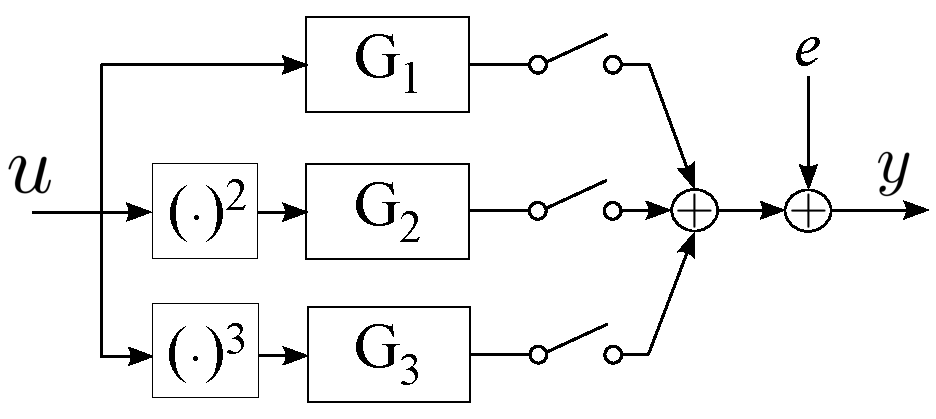
\includegraphics[width=0.5\textwidth]{Chapter7_NOFRFs/ParallelHammNumEx.pdf}
\caption{Parallel Hammerstein structure used for numerical examples}
\label{fig:ParallelHammNumEx}
\end{figure}

In the simulation, the linear filters (and therefore the NOFRFs), $G_1$, $G_2$ and $G_3$, are constructed as Chebyshev filters with resonant modes at normalized frequencies 0.072, 0.111 and 0.091 respectively. The inputs in any given experiment are random-phase multisines which are periodic in $N=128$ samples and have no zero frequency component. The band of excitation, $\mathbf{k}$, for the multisines is constructed so as to avoid aliasing in the output spectrum. The output error, $e$, is a Gaussian white noise vector added in each experiment to provide the required signal-to-noise ratio (SNR).

\subsection{Comparison of traditional and GPR methods}

Four 1000-run Monte Carlo studies are performed on the traditional and regularized estimation methods to determine their relative accuracy.  The studies are:
\begin{enumerate}
\item $M=2$ ($G_1$ and $G_2$ branches) with SNR = 40dB. 1 input/output realization for the \emph{regularized} method. 2 input scalings for the \emph{traditional} method. 
\item $M=2$ ($G_1$ and $G_2$ branches) with SNR = 20dB. 1 input/output realization for the \emph{regularized} method. 2 input scalings for the \emph{traditional} method. 
\item $M=3$ (all branches) with SNR = 40dB. 1 input/output realization for the \emph{regularized} method. 3 input scalings for the \emph{traditional} method. 
\item $M=3$ (all branches) with SNR = 40dB. 10 input/output realizations for the \emph{regularized} method. 10 input scalings for the \emph{traditional} method. 
\end{enumerate}

Note that for studies 1, 2 and 3, the traditional multi-level excitation method uses its minimum requirement of $M$ differently scaled inputs, and hence $M$ experiments. In contrast, the regularized method is disadvantaged in these studies by using only one input and experiment, such that data collection is faster by a factor of $M$. Furthermore, the estimation is performed on a dataset which is smaller by a factor of $M$ for the GPR method. The final study (4) compares the two methods for an equal amount of measurement data, using the results in Section \ref{sec:NOFRF_MultipleRealizations} for the regularized method. For a fair comparison of the two methods, all studies use measurement data taken from the steady-state portion of the experiment, i.e. there are no transient components in the output response. 

To visualize performance in each Monte Carlo study, Figures \ref{fig:NOFRFs_2ndOrder_SNR100}, \ref{fig:NOFRFs_2ndOrder_SNR10}, \ref{fig:NOFRFs_3rdOrder_SNR100} and \ref{fig:NOFRFs_3rdOrder_SNR100_10times} plot the true NOFRF magnitudes as well as the central 95\% intervals (shaded) from each estimation method. For studies 1, 2 and 3, the regularized method produces tighter intervals which are more centered around the true NOFRF, despite having a shorter experiment time and using significantly less data in the estimation. The contrast in performance is even clearer in the results for study 4, where the regularized method is allowed to use an equal amount of measurement data. All of the Monte Carlo results show a clear accuracy benefit for the proposed method when output measurement noise is present in the system, which can be attributed to the ability of GPR methods to significantly reduce estimation covariance at the price of a small bias \citep{Pillonetto2014}. The bias here is small but evident, particularly at the resonance peaks of each NOFRF.

\begin{figure}[!hp]
\centering
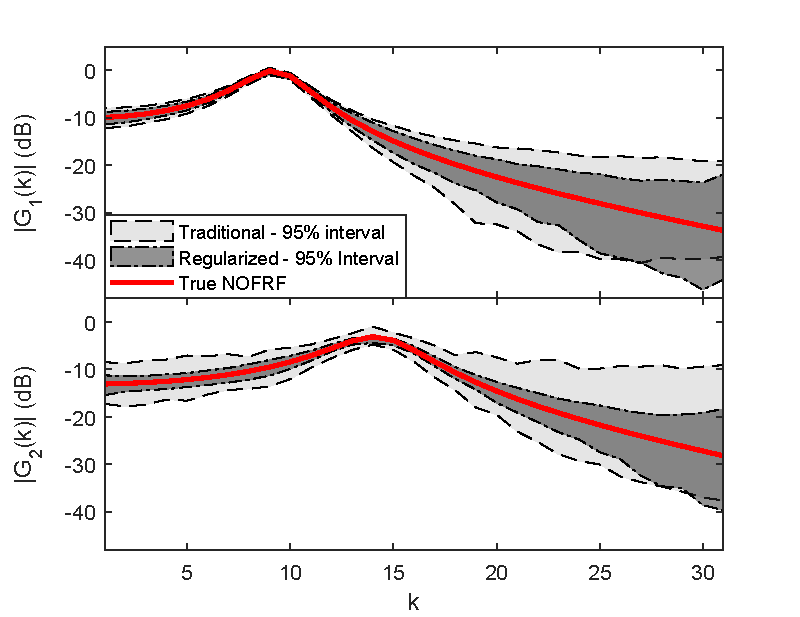
\includegraphics[width=0.8\textwidth]{Chapter7_NOFRFs/Hamm2ndOrder_SNR100_N128_DiscreteTime.pdf}
\caption{Magnitude intervals for study 1, $M=2$ and SNR=40dB}
\label{fig:NOFRFs_2ndOrder_SNR100}
\end{figure}

\begin{figure}[!hp]
\centering
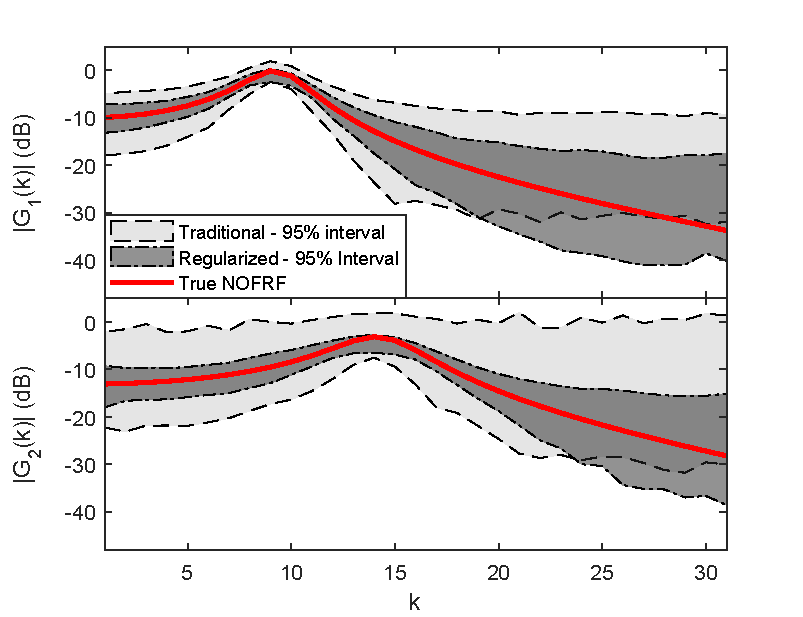
\includegraphics[width=0.8\textwidth]{Chapter7_NOFRFs/Hamm2ndOrder_SNR10_N128_DiscreteTime.pdf}
\caption{Magnitude intervals for study 2, $M=2$ and SNR=20dB}
\label{fig:NOFRFs_2ndOrder_SNR10}
\end{figure}

\begin{figure}[!hp]
\centering
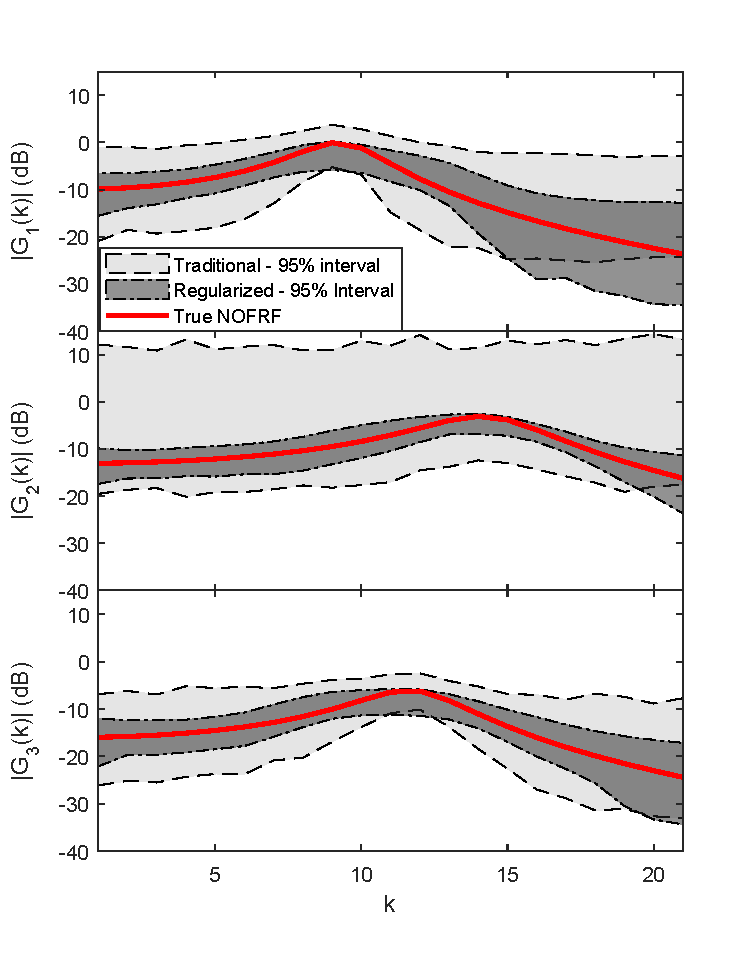
\includegraphics[width=0.6\textwidth]{Chapter7_NOFRFs/Hamm3rdOrder_SNR100_N128_DiscreteTime.pdf}
\caption{Magnitude intervals for study 3, $M=3$ and SNR=40dB}
\label{fig:NOFRFs_3rdOrder_SNR100}
\end{figure}

\begin{figure}[!hp]
\centering
\includegraphics[width=0.6\textwidth]{Chapter7_NOFRFs/Hamm3rdOrder_SNR100_10timesN128_DiscreteTime.pdf}
\caption{Magnitude intervals for study 4, $M=3$ and SNR=40dB (equal data)}
\label{fig:NOFRFs_3rdOrder_SNR100_10times}
\end{figure}

\subsection{Transient estimation test}

While the traditional multi-level excitation method cannot estimate or remove the effect of transients, it was shown in Section \ref{sec:NOFRF_TransientEstimation} that the proposed approach can be modified to consider transient functions in the Gaussian process regression. This allows us to simultaneously estimate the NOFRFs and their corresponding transients, thereby increasing the accuracy of estimation for non-periodic or non steady-state data. 

To demonstrate this capability, the modified method in Section \ref{sec:NOFRF_TransientEstimation} was applied to the simulated system of Figure \ref{fig:ParallelHammNumEx}, using the $G_1$ and $G_2$ branches and no output noise. The input multisine was applied for a single period and preceded by zero initial conditions, producing a transient in the output response. Using this input/output data, the total transient could be estimated by summing the transient estimates from each nonlinear order, i.e.
\begin{equation}
T(k) = \sum_{m=1}^{M} T_m(k).
\end{equation}
The true and estimated transients are plotted in Figure \ref{fig:NOFRFTransientEstimates} for three input realizations, showing reasonable estimation performance which significantly reduces the effect of the transients on NOFRF estimation accuracy. 

\begin{figure}[h]
\centering
\includegraphics[width=0.7\textwidth]{Chapter7_NOFRFs/NOFRF_Transient1.pdf}
\includegraphics[width=0.7\textwidth]{Chapter7_NOFRFs/NOFRF_Transient4.pdf}
\includegraphics[width=0.7\textwidth]{Chapter7_NOFRFs/NOFRF_Transient5.pdf}
\caption{True and estimated transient functions for three input realizations of the test system ($M=2$)}
\label{fig:NOFRFTransientEstimates}
\end{figure}

\section{Conclusion}

This chapter adapts the Bayesian techniques from linear identification theory to the problem of estimating parallel Hammerstein systems in the frequency domain. First, the NOFRF model structure was shown to be an intuitive and useful tool in estimating such systems, since the frequency function at each nonlinear order will be input-independent and pseudo-linear for this case. In developing a GPR method, the Gaussian prior covariances for each frequency function could then be chosen and tuned according to results obtained for linear FRF estimation in~\cite{Lataire2016}. The proposed method was extended to consider concurrent transient estimation in the case of non-steady-state data. When compared to the traditional NOFRF estimation method of multi-level excitation, the proposed method has fewer experimental constraints and can achieve higher accuracy using less data when output noise is present. 

In order to estimate frequency domain models for a broader class of nonlinear systems, the NOFRF method proposed in this chapter would not be sufficient. This is because the NOFRFs are input-dependent in general, and thus we cannot always impose prior covariance structures borrowed from the linear theory. An alternate option is to move to the multidimensional GFRF model structure, and design an analogous method to the regularized Volterra kernel estimation outlined in Chapter \ref{sec:RegVolterraTD}. Such an approach will be considered in Chapter \ref{chap:8}.

\cleardoublepage
\chapter{Gaussian Process Regression for the Estimation of Generalized Frequency Response Functions}
\label{chap:8}
\emph{The generalized frequency response function (GFRF) model is the most direct frequency domain equivalent to the time domain Volterra series, where each GFRF is a multidimensional Fourier transform of the corresponding Volterra kernel. This chapter develops a Gaussian process regression (GPR) method for data-driven identification of GFRF models. Each GFRF is modeled as a real/complex Gaussian process with prior covariance related to the time domain characteristics of its corresponding Volterra kernel, such that the method is a frequency domain equivalent of the Bayesian regularization method considered in Part \ref{part:TD}. Numerical examples highlight the benefit, when only a limited frequency band is of interest, of using the proposed direct approach over indirect estimation from a time domain model.}
\newpage
\section{Introduction}

In Part \ref{part:FD} of this thesis, we are considering Bayesian estimation of Volterra series models in the frequency domain. While Chapter \ref{chap:7} revealed that Gaussian process regression (GPR) can be applied to the NOFRF model, the results were limited to the case of a parallel Hammerstein nonlinear system, as this is the case where the NOFRFs become input independent and thus easy to model in a Bayesian sense. In order to make Bayesian frequency domain estimation more broadly applicable, it is necessary to move to the generalized frequency response function (GFRF) model, where each complex-valued GFRF in the series is related to its corresponding time domain kernel through a multidimensional Fourier transform.

The estimation of GFRFs has been extensively studied in the literature. In one case, an interpolation method for the second order term was developed \cite{Nemeth2002}, which requires multiple input realizations to give an overdetermined problem. Other studies utilized excitations with specifically selected harmonics, however such methods become prohibitively complex for high nonlinear orders, and there is a limit to the number of GFRF elements which can be estimated~\cite{Boyd1983}, \cite{Evans1996}. Alternatively, full GFRF estimates can be obtained from arbitrary excitation by first identifying the time domain Volterra kernels and then transforming to the frequency domain \cite{Vlaar2018}. In the case where a limited frequency band is of interest, then identification directly in the frequency domain is more beneficial with respect to the number of estimated parameters.

The contribution of this chapter is to develop a frequency domain GFRF identification method using GPR, and thus further expand the capabilities of nonparametric Bayesian estimation. As in previous chapters, concepts from \cite{Birpoutsoukis2017} and \cite{Lataire2016} will serve as inspiration in developing the method. In particular, the real/complex Gaussian framework described in Chapter \ref{sec:RCN} is utilized again, and the GFRFs are modeled using prior covariances translated from the time domain functions designed in \cite{Birpoutsoukis2017}.

The proposed approach can obtain GFRF estimates up to an arbitrary nonlinear order using a single multisine input excitation, even though the estimation problem is severely rank deficient. For cases where only a limited frequency band is of interest, the proposed method presents a clear advantage over indirect time domain GPR, which is a property that was also observed for the linear case in \cite{Lataire2016}.

\section{Problem formulation}
\label{sec:ProblemFormulation_GFRFs}

For convenience, the relevant time domain and frequency domain Volterra models will be recalled here for reference throughout the chapter. The original time domain series is given by
\begin{equation}
\begin{split}
y^0(t) &= h_0 + \sum_{m=1}^M y_m(t), \\
y_m(t) &= \sum_{\tau_1 = 0}^{n_m-1} \hdots \sum_{\tau_m=0}^{n_m-1} h_m(\tau_1, \hdots, \tau_m) \prod_{\tau=\tau_1}^{\tau_m} u(t-\tau).
\end{split}
\label{eq:VolterraTimeDomainOutput_GFRFs}
\end{equation}
The GFRF model then relates the (steady-state) input and output spectrum in the frequency domain, i.e.
\begin{equation}
\begin{split}
Y^0(k) &= H_0(k) + \sum_{m=1}^{M} Y_m(k),  \\
Y_m(k) &= \frac{1}{N^{m-1}} \sum_{k_1 + \hdots + k_m = k} H_m(k_1, \hdots,k_m) \prod_{i=1}^{m} U(k_i), 
\end{split}
\label{eqn:GFRFoutputeqn_GFRFs}
\end{equation}
where the GFRFs, $H_m$, are obtained via multidimensional Fourier transforms on the corresponding Volterra kernels, $h_m$, using
\begin{equation}
\label{eqn:GFRF_Transform_GFRFs}
H_m(k_1, \hdots,k_m) = \sum_{\tau_1=0}^{n_m - 1} \hdots \sum_{\tau_m=0}^{n_m-1} h_m(\tau_1,\hdots,\tau_m) e^{\frac{-j2 \pi k_1 \tau_1}{N}} \cdots e^{\frac{-j2 \pi k_m \tau_m}{N}}.
\end{equation}

The nonlinear system identification problem is now formulated in the frequency domain under steady-state conditions, using the following assumptions and notation: 
\begin{assum}
\label{assum:white_noise_Volterra_output}
The measured output, $\{y(t)\}_{t=0}^{N-1}$, is a Volterra output corrupted by white noise, i.e.
\begin{equation}
y(t) = y^0(t) + e(t); \; \; \; \; e(t) \sim \mathcal{N}(0,\sigma^2),
\label{eqn:VolterraWithNoise_transients}
\end{equation}
where $y^0(t)$ is the noise-free Volterra output from (\ref{eq:VolterraTimeDomainOutput_GFRFs}).
\end{assum}
\begin{assum}[Steady-state]
The measured input $\{u(t)\}_{t=0}^{N-1}$ is one period of an N-periodic sequence which has been applied to the system for a sufficiently long time  such that the system is in steady-state with a corresponding N-periodic output response, $\{y^0(t)\}_{t=0}^{N-1}$, whose spectrum can be given by the steady-state GFRF model (\ref{eqn:GFRFoutputeqn_GFRFs}).
\label{assum:steadystate_transients}
\end{assum}
%\begin{assum}[Alias-free]
%\label{assum:antialias_input}
%The input DFT spectrum for non-negative frequencies, $\{U(k): k \in \mathbb{Z}, 0 \leq k \leq N/2\}$, has non-zero values only in the set of indices $\mathbf{k_u} \subset \{0,\hdots,\floor*{\frac{N}{2M}} \}$, where $\floor*{\cdot}$ is the floor operator.
%\end{assum}
\begin{notation}
The set of DFT indices, $k$, for which the input spectrum, $\{U(k): k \in \mathbb{Z}, 0 \leq k \leq N/2\}$, is non-zero is denoted by $\mathbf{k_u}$. Likewise, the set of indices for which the output spectrum, $\{Y(k): k \in \mathbb{Z}, 0 \leq k \leq N/2\}$, is non-zero (due to input excitation) is denoted by $\mathbf{k_y}$ (see \cite{Lang1997} for the precise definition of this set for a given $U(k)$ and $M$).
\end{notation}
\begin{notation}
The frequencies of interest for estimation are given by the set \begin{equation} \mathbf{k_e} = -\mathbf{k_u} \cup \mathbf{k_u}. \end{equation}
\end{notation}
Given Assumptions \ref{assum:white_noise_Volterra_output} and \ref{assum:steadystate_transients}, the goal is to estimate the GFRF elements, $H_0$ and $H_m(k_1, \hdots,k_m)$ $\forall k_1, \hdots,k_m \in \mathbf{k_e}$ and $m = 1,\hdots,M$.

\section{Gaussian process regression for GFRFs}
\label{sec:GPR_GFRFs}

Given the assumptions and problem formulation described in Section \ref{sec:ProblemFormulation_GFRFs}, a GPR method is developed in this section. The hybrid real/complex normal distribution will be required for this purpose, since every GFRF contains both complex \emph{and} strictly real components. Thus, the notation and properties introduced in Chapter \ref{sec:RCN} will also be used in this chapter.

\subsection{GFRFs as real/complex Gaussian vectors}

Any set of GFRF parameters can be arranged into a real/complex vector, as outlined in the following definition.

\begin{defn}
The $m$-dimensional array containing $H_m(k_1, \hdots,k_m), \ \forall k_1, \hdots,k_m \in \mathbf{k_e}$ has a real/complex vectorized form (shown in (\ref{eqn:RCG_vector_defn})) which will be denoted by 
\begin{equation}
\label{eqn:GFRF_RCG_vector}
H_m^{\mathcal{V}} = \begin{bmatrix} H_m^{\mathbb{R}} \\ H_m^{\mathbb{C}} \end{bmatrix}, 
\end{equation}
where $H_m^{\mathbb{R}}$ contains the strictly real components.
\end{defn}

Unlike in \cite{Lataire2016} and Chapter \ref{chap:7}, where the one-dimensional frequency functions are strictly real only at zero frequency, higher order GFRFs originating from symmetric Volterra kernels present a larger set of real components. Since we are required to express the vectorized GFRFs in the form dictated by (\ref{eqn:GFRF_RCG_vector}), it is important to identify the location of all strictly real elements, as addressed in the following theorem.

\begin{thm}
\label{thm:GFRF_real_elements}
Consider a symmetric $m$\textsuperscript{th} order Volterra kernel, $h_m(\tau_1, \hdots, \tau_m)$, as defined in (\ref{eq:VolterraTimeDomainOutput_GFRFs}), and its corresponding GFRF, $H_m(k_1, \hdots,k_m)$, as defined in (\ref{eqn:GFRF_Transform_GFRFs}). The strictly real components of $H_m$ are defined by the set of DFT indices,
\begin{align*}
\mathbf{k}_m^{\mathbb{R}} = \{k_1, \hdots, k_m \in \mathbb{Z}: \sum_{\mathcal{I} \in S_m(X)} \sin \bigg( \frac{2 \pi}{N} (k_1 \tau_{i_1} + \hdots + k_m \tau_{i_m}) \bigg) = 0 \; \; \forall \tau_i \in \mathbb{N} \}, 
\end{align*}
where $\mathcal{I} = [i_1, \hdots, i_m]$, and $S_m(X)$ denotes the set of all permutations of the vector $X = [1, 2, \hdots,m]$.
\end{thm}
\begin{proof*}
Taking the imaginary part of (\ref{eqn:GFRF_Transform_GFRFs}), we obtain
\begin{align}
\mathfrak{I} \{ &H_m(k_1,\hdots,k_m) \} = \sum_{\tau_1 = 0}^{n_m-1} \hdots \sum_{\tau_m = 0}^{n_m-1} h_m(\tau_1,\hdots,\tau_m) \sin(\frac{2 \pi}{N}(k_1 \tau_1 + \hdots + k_m \tau_m)).
\end{align}
For a symmetric kernel $h_m$, the Fourier transformation will be independent of the ordering of the lags, $\tau_1,\hdots,\tau_m$, so it is equivalent to take an average over all lag permutations,
\begin{align}
\mathfrak{I} \{ &H_m(k_1,\hdots,k_m) \} \nonumber \\
&= \frac{1}{m!} \sum_{\mathcal{I} \in S_m(X)} \Bigg[ \sum_{\tau_1 = 0}^{n_m-1} \hdots \sum_{\tau_m = 0}^{n_m-1} h_m(\tau_{i_1},\hdots,\tau_{i_m}) \sin \bigg( \frac{2 \pi}{N}(k_1 \tau_{i_1} + \hdots + k_m \tau_{i_m}) \bigg) \Bigg] \\
&= \frac{1}{m!} \sum_{\tau_1 = 0}^{n_m-1} \hdots \sum_{\tau_m = 0}^{n_m-1} h_m(\tau_{1},\hdots,\tau_{m}) \sum_{\mathcal{I} \in S_m(X)} \sin \bigg( \frac{2 \pi}{N}(k_1 \tau_{i_1} + \hdots + k_m \tau_{i_m}) \bigg).
\end{align}
Thus, for an arbitrary symmetric $h_m$, strictly real elements of $H_m$ are guaranteed only when
\begin{align*}
\sum_{\mathcal{I} \in S_m(X)} \sin(\frac{2 \pi}{N}(k_1 \tau_{i_1} + \hdots + k_m \tau_{i_m})) = 0 \; \; \forall \tau_i \in \mathbb{N} 
\end{align*} 
as required. \hfill $\qed$
\end{proof*}

To explicitly locate the strictly real elements within the estimation set, $\mathbf{k_e}$, the result in Theorem \ref{thm:GFRF_real_elements} can be elaborated using the antisymmetry of $\sin()$, as shown below for the first three nonlinear orders. %(i.e. the orders considered in the simulation examples).
\begin{align}
\mathbf{k}_1^{\mathbb{R}} = &\{k_1 \in \mathbf{k_e}: k_1 = 0 \}, \\
\mathbf{k}_2^{\mathbb{R}} = &\{k_1, k_2 \in \mathbf{k_e}: k_1 = -k_2 \}. \\
\mathbf{k}_3^{\mathbb{R}} = &\{k_1,k_2,k_3 \in \mathbf{k_e}: k_1 = -k_2, k_3 = 0 \} \cup \nonumber \\
& \hspace{10mm} \{k_1,k_2,k_3  \in \mathbf{k_e}: k_1 = -k_3, k_2 = 0 \} \cup \nonumber \\
& \hspace{20mm} \{k_1,k_2,k_3  \in \mathbf{k_e}: k_2 = -k_3, k_1 = 0 \}. 
\end{align}
Note that the set for the first order GFRF, $\mathbf{k}_1^{\mathbb{R}}$, can only contain the zero frequency entry, as is the case for a linear FRF. The multidimensional GFRFs, however, possess larger sets in general.

\subsection{The Gaussian assumption}

The following Gaussian assumptions are placed on the vectorized GFRF quantities, $H_m^{\mathcal{V}}$.  
\begin{assum}
\label{GFRF_GaussianAssumption}
$H_m^{\mathcal{V}}$ is real/complex normally distributed with zero mean and augmented covariance $\Sigma_m$, i.e.
\begin{equation} 
\label{GFRF_GaussianDefn}
H_m^{\mathcal{V}} \sim \mathcal{RCN}(0,\Sigma_m) ,
\end{equation}
where $\Sigma_m$ is constructed from the covariance and relation functions $R_m$, $Q_m$, $K_m$ and $C_m$ as in (\ref{eqn:augmented_covariance}).
\end{assum}
\begin{assum}
\label{GFRF_IndependenceAssumption}
Two (real/complex vectorized) Gaussian GFRFs of different orders are independent, i.e. $H_i^{\mathcal{V}}$ and $H_j^{\mathcal{V}}$ are independent for $i \neq j$.
\end{assum}
The assumptions \ref{GFRF_GaussianAssumption} and \ref{GFRF_IndependenceAssumption} are consistent with those made in \cite{Birpoutsoukis2017} and \cite{Lataire2016}, as well as in previous chapters of this thesis. They will be used in the sequel to derive the output spectrum distribution and define the GPR procedure for GFRF estimation.

\subsection{Prior covariance design}

For multidimensional Volterra kernels, prior covariance functions have already been constructed in the time domain \cite{Birpoutsoukis2017}, \cite{Birpoutsoukis2017c}, by applying a TC or DC structure along multiple perpendicular regularizing directions. The same approach was adopted for the time domain methods in this thesis, in Chapters 4, 5 and 6. The resulting covariance matrices are guaranteed to be valid and produce stable kernel realizations.

In order to construct a frequency domain analog to the Volterra kernel covariance function, we note that there exists a linear transformation between the vectorized kernel $h_m^{\mathcal{V}}$ and its frequency domain counterpart, $H_m^{\mathcal{V}}$, which will be denoted $F_m$, i.e.
\begin{equation}
H_m^{\mathcal{V}} = \begin{bmatrix} H_m^{\mathbb{R}} \\ H_m^{\mathbb{C}} \end{bmatrix} = \begin{bmatrix} F_m^{\mathbb{R}} \\ F_m^{\mathbb{C}} \end{bmatrix} h_m^{\mathcal{V}} = F_m h_m^{\mathcal{V}},
\end{equation}
where $F_m^{\mathbb{R}}$ produces $H_m^{\mathbb{R}}$ and $F_m^{\mathbb{C}}$ produces $H_m^{\mathbb{C}}$. While it is clear from (\ref{eqn:GFRF_Transform_GFRFs}) that $F_m$ should contain appropriate products of exponentials, a more rigorous approach for obtaining the explicit form of $F_m$ and its submatrices requires the following theorem.

\begin{thm}
\label{thm:ND-DFTs}
Consider the m-dimensional array $w_m \in \mathbb{R}^{N \times \hdots \times N}$, and its m-dimensional DFT, $W_m \in \mathbb{C}^{N \times \hdots \times N}$. Consider also their vectorized forms, $w_m^{\mathcal{V}}\in \mathbb{R}^{N^{m}}$ and $W_m^{\mathcal{V}} \in \mathbb{C}^{N^{m}}$, where vectorization is performed such that 
\begin{align*}
w_m^{\mathcal{V}} = \big[ w_m(1,1,\hdots,1), &w_m(2,1,\hdots,1),\hdots, \\
& \; \; w_m(N,1,\hdots,1), w_m(1,2,\hdots,1), \hdots, w_m(N,N,\hdots,N) \big],
\end{align*}
and likewise for $W_m^{\mathcal{V}}$. The vectorized arrays are related by,
\begin{equation}
W_m^{\mathcal{V}} = \Psi_m w_m^{\mathcal{V}},
\end{equation}
where $\Psi_m$ can be obtained from the recursive definition,
\begin{align}
\Psi_p = \Psi_{p-1} \otimes \Psi_1,  \; \; p = 2, 3, \hdots, m  
\end{align}
and where $\Psi_1$ is the $N \times N$ DFT matrix.
\end{thm}

\begin{proof*}
For $m=1$, by definition we have:
\begin{equation}
W_1^{\mathcal{V}} = \Psi_1 w_1^{\mathcal{V}}
\end{equation}
For $m=2$, the DFT is applied in each dimension separately:
\begin{align}
W_2 &= \Psi_1 w_2 \Psi_1^T \\
&= \underbrace{[\Psi_1 \otimes \Psi_1]}_{\Psi_2} w_2^{\mathcal{V}},
\end{align}
by the well known property of Kronecker products. 

For tensor $W_m = \{ W_{i_1,\hdots,i_m} \}_{i_1,\hdots,i_m = 0}^{N-1}$, let the $m-1$ dimension tensor $W_m^{(k)}$ be given by $\{ W_{i_1,\hdots,i_{m-1},k} \}_{i_1,\hdots,i_{m-1} = 0}^{N-1}$. 

Assuming $W_{p-1}^{\mathcal{V}} = \Psi_{p-1} w_{p-1}^{\mathcal{V}}$, then by induction:
\begin{align}
\big[ {W_{p}^{(1)}}^{\mathcal{V}} \; \hdots \; {W_{p}^{(N)}}^{\mathcal{V}} \big]  &= \big[ \Psi_{p-1} {w_{p}^{(1)}}^{\mathcal{V}} \; \hdots \; \Psi_{p-1} {w_{p}^{(N)}}^{\mathcal{V}} \big] \Psi_1^T \\
&= \Psi_{p-1} \big[ {w_{p}^{(1)}}^{\mathcal{V}} \; \hdots \; {w_{p}^{(N)}}^{\mathcal{V}} \big] \Psi_1^T \\
\implies W_{p}^{\mathcal{V}} &= \underbrace{[\Psi_{p-1} \otimes \Psi_1]}_{\Psi_{p}} w_{p}^{\mathcal{V}}
\end{align}
again using the Kronecker product property. Thus, $\Psi_{p} = \Psi_{p-1} \otimes \Psi_1 $ as required \hfill  $\qed$

\end{proof*} 

Assuming $h_m^{\mathcal{V}}$ is vectorized as described in Theorem \ref{thm:ND-DFTs}, we can form $F_m$ by first computing the matrix $\Psi_m$, then rearranging and removing rows to correspond to a desired vectorization of $H_m^{\mathcal{V}}$ which satisfies the required form in (\ref{eqn:GFRF_RCG_vector}).

The transformation can now be used to convert time domain covariance functions to the frequency domain,
\begin{equation}
\begin{split}
R_m &= \textbf{E} \{ H_m^{\mathbb{R}} {H_m^{\mathbb{R}}}^T\} = F_m^{\mathbb{R}} \textbf{E} \{ h_m^{\mathcal{V}} {h_m^{\mathcal{V}}}^T \} {F_m^{\mathbb{R}}}^T = F_m^{\mathbb{R}} P_m {F_m^{\mathbb{R}}}^T \\
Q_m &= \textbf{E} \{ H_m^{\mathbb{R}} {H_m^{\mathbb{C}}}^H\} = F_m^{\mathbb{R}} \textbf{E} \{ h_m^{\mathcal{V}} {h_m^{\mathcal{V}}}^T \} {F_m^{\mathbb{C}}}^H = F_m^{\mathbb{R}} P_m {F_m^{\mathbb{C}}}^H \\
K_m &= \textbf{E} \{ H_m^{\mathbb{C}} {H_m^{\mathbb{C}}}^H\} = F_m^{\mathbb{C}} \textbf{E} \{ h_m^{\mathcal{V}} {h_m^{\mathcal{V}}}^T \} {F_m^{\mathbb{C}}}^H = F_m^{\mathbb{C}} P_m {F_m^{\mathbb{C}}}^H \\
C_m &= \textbf{E} \{ H_m^{\mathbb{C}}{H_m^{\mathbb{C}}}^T\} = F_m^{\mathbb{C}} \textbf{E} \{ h_m^{\mathcal{V}} {h_m^{\mathcal{V}}}^T \} {F_m^{\mathbb{C}}}^T = F_m^{\mathbb{C}} P_m {F_m^{\mathbb{C}}}^T 
\end{split}
\label{eq:CovarianceRelationTransforms_GFRFs}
\end{equation}
where $P_m =  \textbf{E} \{ h_m^{\mathcal{V}} {h_m^{\mathcal{V}}}^T \}$ denotes the tunable TC/DC-based covariance structure designed in~\cite{Birpoutsoukis2017} and discussed in Chapter \ref{sec:RegVolterraTD} of this thesis.

The full augmented covariance, $\Sigma_m$, for the $m$\textsuperscript{th} GFRF is constructed as in (\ref{eqn:augmented_covariance}), i.e.
\begin{equation}
\Sigma_m = \begin{bmatrix}  R_m & Q_m & \overline{Q_m} \\ {Q_m}^H & K_m & C_m \\ \overline{{Q_m}^H} & {C_m}^H & \overline{K_m}\end{bmatrix}. \label{eqn:augmented_covariance_GFRFs}
\end{equation} 

\begin{rem}
In practice, symmetry must be enforced in both the time and frequency domain kernels to guarantee a unique Volterra series representation \cite{Schetzen1980}. Thus, we are required to modify the transformation matrices, $F_m$, by removing the columns which correspond to redundant time domain parameters, and removing rows that correspond to redundant frequency domain parameters. As an example, see Figure \ref{fig:BandLimitedVisual} in Section \ref{sec:FDvsTD_GFRFs} for the symmetry axes of a second order kernel and GFRF, which are used to dictate the location of unique and redundant parameters in those series terms.  
\end{rem}

\subsection{Deriving the MAP estimate}

First we must derive the output spectrum distribution for $Y(\mathbf{k_y})$, which requires the restructuring of the model equation (\ref{eqn:GFRFoutputeqn_GFRFs}) into the regression form,
\begin{align}
Y(\mathbf{k_y}) &=  [\Phi_1 \hdots \Phi_M] [{H_1^{\mathcal{V}}}^T \hdots {H_M^{\mathcal{V}}}^T]^T + E(\mathbf{k_y}) \nonumber \\
&= \Phi H + E,
\label{eqn:GFRF_OutputSpectrum}
\end{align}
where $E$ is the (assumed) i.i.d. error vector in the frequency domain, and $\Phi_m$ is an appropriate regressor containing the input spectrum products corresponding to $H_m^{\mathcal{V}}$. Note that symmetry should also be enforced in the GFRFs here, which should be reflected in the design of the regressors. 

Now $Y(\mathbf{k_y})$, being formed from the DFT of the real signal $y(t)$, will also be a real/complex vector in the case where $0 \in \mathbf{k_y}$. Thus, we extend (\ref{eqn:GFRF_OutputSpectrum}) to the augmented output case, resulting in
\begin{align}
\label{AugmentedModel}
\widetilde{Y}(\mathbf{k_y}) &=  [\widetilde{\Phi_1} \hdots \widetilde{\Phi_M}] [\widetilde{H_1^{\mathcal{V}}}^T \hdots \widetilde{H_M^{\mathcal{V}}}^T]^T + \widetilde{E}(\mathbf{k_y}) \nonumber \\
&= \widetilde{\Phi}\widetilde{H} + \widetilde{E}.
\end{align}
The augmented regressors can be constructed as
\begin{equation}
\widetilde{\Phi_m} = \begin{bmatrix}\Phi_m^{\mathbb{R}} & \Phi_m^{\mathbb{RC}} & 0 & 0 \\0 & 0 & \Phi_m^{\mathbb{C}} & 0 \\ 0 & 0 & 0 & \overline{\Phi_m^{\mathbb{C}}} \end{bmatrix},
\end{equation}
where $\Phi_m^{\mathbb{R}}$ maps the contribution of $H_m^{\mathbb{R}}$ to $Y(0)$, and $\Phi_m^{\mathbb{RC}}$ maps the contribution to $Y(0)$ from complex GFRF components. Note that this formulation dictates (to some extent) the required ordering of the vector $H_m^{\mathcal{V}}$. 

\begin{rem}
\label{rem:GFRF_RankDeficiency}
When $\Phi$ is constructed from a single input/output realization as in (\ref{eqn:GFRF_OutputSpectrum}), the associated linear regression problem will be severely rank deficient for $M>1$. While it is possible to make the problem overdetermined by `stacking' a sufficient number of unique input/output realizations (similarly to Chapter \ref{sec:NOFRF_MultipleRealizations}), we will focus on the rank deficient case in this chapter to highlight the flexibility of GPR.
\end{rem}

From (\ref{AugmentedModel}), the output spectrum distribution is derived as follows.
\begin{thm}
For a system whose output is given by (\ref{eqn:VolterraWithNoise_transients}), with Gaussian $H_m^{\mathcal{V}} \sim \mathcal{RCN}(0,\Sigma_m)$ as described in (\ref{GFRF_GaussianDefn}), the output spectrum $Y(\mathbf{k_y})$ is real/complex normally distributed as follows,
\begin{equation}
\begin{split}
\label{OutputSpectrumThm}
Y(\mathbf{k_y}) &\sim \mathcal{RCN}(0,\Sigma_Y), \\
\text{where } \Sigma_Y &= \widetilde{\Phi}\Sigma_{tot} \widetilde{\Phi}^H + \sigma^2 I \\
\text{and } \Sigma_{tot} &= \begin{bmatrix} \Sigma_1 & &0 \\ & \ddots & \\ 0 & & \Sigma_M \end{bmatrix}.
\end{split}
\end{equation}
\end{thm}

\begin{proof*}
Follows directly from (\ref{AugmentedModel}), Assumptions \ref{assum:white_noise_Volterra_output}, \ref{GFRF_GaussianAssumption} and \ref{GFRF_IndependenceAssumption}, and the properties of real/complex normal distributions. \hfill $\qed$
\end{proof*}

Finally, maximum a posteriori (MAP) estimates for the GFRFs can be obtained from the joint distribution of $Y$ and $H$, by computing the mean of the conditional distribution $H|Y$. The result is provided in the following theorem.

\begin{thm}
The MAP estimate of $\widetilde{H}$ in (\ref{AugmentedModel}) is
\begin{equation}
\label{eqn:GFRF_MAP}
\hat{{\widetilde{H}}}_{MAP} = \Sigma_{tot} \widetilde{\Phi}^H \Sigma_Y^{-1} \widetilde{Y}
\end{equation}
\end{thm}

\begin{proof*}
Follows from the properties of real/complex normal distributions \cite{Lataire2016}. \hfill $\qed$
\end{proof*}

\subsection{Hyperparameter tuning}

We must optimize the hyperparameters, $\eta$, describing each covariance function $P_m(\eta)$, which are in turn used to construct $\Sigma_m$ in (\ref{eq:CovarianceRelationTransforms_GFRFs}). As in \cite{Birpoutsoukis2017} and \cite{Lataire2016}, this chapter will use a marginal likelihood maximization (MLM), i.e.
\begin{equation}
\label{eqn:GFRF_hyperparam_tuning}
\hat{\eta} = \text{arg } \underset{\eta}{\text{min }} \widetilde{Y}(\mathbf{k_y})^H \Sigma_Y^{-1}(\eta) \widetilde{Y}(\mathbf{k_y}) + \text{log det } \Sigma_Y(\eta).
\end{equation}

\begin{rem}
The disadvantages of using a MLM approach were highlighted in Chapter \ref{chap:4} for the time domain case. The same situation exists in the frequency domain for GFRFs, i.e. the dimension of the search space in (\ref{eqn:GFRF_hyperparam_tuning}) grows quadratically with the maximum nonlinear order, $M$, and hence the computational burden for the optimization grows even more rapidly. An equivalent EM approach to that of Algorithm \ref{alg:EMtuning} in Chapter \ref{chap:4} can be derived, in an almost identical fashion, for the GFRF estimation problem. The EM tuning method is recommended when $M$ is large.
\end{rem}

\subsection{Comparison with the indirect time domain approach}
\label{sec:FDvsTD_GFRFs}

There is another viable approach for estimating GFRFs under rank deficient conditions, which is to first compute regularized Volterra kernel estimates in the time domain with memory length $n_m = N$, and subsequently transform them using (\ref{eqn:GFRF_Transform_GFRFs}). One advantage of this indirect approach is the freedom to use input/output measurements of arbitrary length which are not necessarily at steady-state, whereas the method proposed here requires such constraints. 

If we are only interested in GFRF estimation for a \emph{specific frequency band}, then the time domain approach has a severe disadvantage when compared to the frequency domain method proposed here. With an indirect time domain approach, we are required to estimate the full set of kernel parameters regardless of frequency band, since each frequency domain parameter depends on the \emph{entire} time domain set (see (\ref{eqn:GFRF_Transform_GFRFs})). In direct frequency domain estimation, the limited frequency band directly reduces the set of parameters to be estimated, and the magnitude of reduction grows rapidly with increasing GFRF order, $m$, since the band is limited along every dimension of the GFRFs. 

An example of this parameter reduction concept is visualized in Figure \ref{fig:BandLimitedVisual} for a second order example with $N=n_2=21$. We excite a discrete set of frequencies, $\mathbf{k_u} = \{ 3,4,5,6,7 \}$, and compare the number of parameters requiring estimation in each domain. It is clear that limiting the excited frequency band in two dimensions significantly reduces the parameter set for $H_2$ to 55 parameters (5 real, 25 complex), while for $h_2$ the full set of unique Volterra coefficients (231 real) is still required.

\begin{figure}[h]
\centering
\includegraphics[width = 0.85\textwidth]{Chapter8_GFRFs/LimitedBandParams_paper.pdf}
\caption{Parameters requiring estimation in second order band-limited example where $\mathbf{k_u} = \{ 3,4,5,6,7 \}$, using a time domain approach (left) and using a direct frequency domain approach (right)}
\label{fig:BandLimitedVisual}
\end{figure}

\section{Simulation examples}

Two simulation studies are presented here in order to demonstrate the performance of the proposed method. The first study considers GFRF estimation in a noise-free setting, but using only period of a multisine excitation such that the problem is severely rank-deficient. In the second study, measurement noise is included and the frequencies of interest are limited to a narrow band. For this case a Monte Carlo study is used to compare the proposed GPR method against an indirect time domain approach. 

\subsection{Study 1: rank deficient noise-free case}
\label{sec:GFRF_noisefree_ex}

In the first study, Volterra system outputs are generated using the block structures in Figure \ref{fig:GFRF_WienerStructure}, where the left structure (a) is in a parallel Wiener configuration, and the right structure (b) has a parallel Hammerstein configuration. The linear filters in each structure are defined in the $z$-domain as
$$G_1(z) = \frac{3z}{z^2 -1.8z + 0.84}, \; \; \;  G_2(z) = 0.25 G_1(z).$$
The input, $u(t)$, is given by a periodic multisine with period $N = 80$ and $\mathbf{k_u} = \{0, 1, 2, \hdots, 19\}$, which is applied for 10 periods before taking the final period of measurements for estimation purposes, such that all transient effects are essentially negligible. 

\begin{figure}[!h]
\centering
\includegraphics[width = 1\textwidth]{Chapter8_GFRFs/ParallelWienerAndHamm_GFRFs.pdf}
\caption{System structures used for data generation in the rank deficient noise-free case}
\label{fig:GFRF_WienerStructure}
\end{figure}

We consider identification of each system's nonzero GFRFs, $H_1$ and $H_2$, assuming memory lengths $n_1=n_2=N$. The resulting estimation problems are severely rank deficient, with 780 unique parameters requiring estimation, and only 77 corresponding output spectrum measurements. Applying the proposed GPR method, the GFRF estimates are given in Figures \ref{fig:GFRF_Noisefree_estimates} (for structure (a)) and \ref{fig:GFRF_Noisefree_estimates_b} (for structure (b)) alongside the true GFRFs, which can be obtained analytically from the system structure (see Chapter \ref{sec:BlockStructureRelationship}). Despite severe rank deficiency, it is clearly seen that a good result is achieved for each system at both GFRF orders.  

\begin{figure}[!h]
\centering
\includegraphics[width = 1.05\textwidth]{Chapter8_GFRFs/WienerExampleEstimates_split2.pdf}
%\caption{First order GFRF estimate (left) and selected slices of the second order GFRF estimate (right)}
\caption{Structure (a) - magnitude plots for the first order GFRF estimate (left), true 2nd order GFRF (middle) and 2nd order estimate for unique parameters (right)}
\label{fig:GFRF_Noisefree_estimates}
\end{figure}

\begin{figure}[!h]
\centering
\includegraphics[width = 1.05\textwidth]{Chapter8_GFRFs/HammersteinExampleEstimates_split.pdf}
%\caption{First order GFRF estimate (left) and selected slices of the second order GFRF estimate (right)}
\caption{Structure (b) - magnitude plots for the first order GFRF estimate (left), true 2nd order GFRF (middle) and 2nd order estimate for unique parameters (right)}
\label{fig:GFRF_Noisefree_estimates_b}
\end{figure}

\subsection{Study 2: limited frequency band with measurement noise}

\begin{figure}[!h]
\centering
\includegraphics[scale = 0.8]{Chapter8_GFRFs/WienerHamm_GFRFs.pdf}
\caption{Wiener-Hammerstein structure used in the limited frequency band MC study}
\label{fig:GFRF_WienerHammStructure}
\end{figure}

To highlight the advantage of the proposed method over an indirect time domain approach, a Monte Carlo (MC) study is also performed. The noise-free outputs are generated using the Wiener-Hammerstein structure in Figure \ref{fig:GFRF_WienerHammStructure}, with linear filters,
$$G_1(z) = \frac{z-1}{z}, \; \; \;  G_2(z) = \frac{1.07z}{z^2 - 1.72 z + 0.77}.$$
The input is a multisine with period $N=55$ and a limited band of excited frequencies, $\mathbf{k_u} = \{ 4,5,\hdots,12 \}$. The output, $y^0$, is disturbed by additive white measurement noise. Note that the system structure can be represented using a single GFRF, $H_2$, as was discussed in Chapter \ref{sec:BlockStructureRelationship}. We will assume for estimation that $n_2 = N$.   

For the MC study we consider three different noise levels, with each noise level having 100 input/output realizations. For each realization, transient-free estimation data is obtained in the same manner as in Section \ref{sec:GFRF_noisefree_ex}. Estimation of the $H_2$ parameters within the excited band is performed using two separate methods:
\begin{enumerate}
\item \textbf{GPR-FD} - GPR in the frequency domain as developed in this chapter (i.e. using (\ref{eqn:GFRF_MAP}) and (\ref{eqn:GFRF_hyperparam_tuning})), and using the DC structure (\ref{DCext}) for each $P_m$.
\item \textbf{GPR-TD} - GPR in the time domain as presented in \cite{Birpoutsoukis2017} using the DC structure for $P_m$, and using periodicity to define the initial conditions $u(t)$ for $t<0$. GFRF parameters are obtained by the DFT transformation (\ref{eqn:GFRF_Transform_GFRFs}) on each time domain kernel, followed by the elimination of parameters not relevant to the frequency band of interest. 
\end{enumerate}
The noise, $e(t)$, is added in each realization to achieve a Signal-to-Noise Ratio (SNR) of 5, 10 or 20dB.

Estimation errors for each method  and realization are quantified using a normalized mean square error (NMSE) metric, given by 
$$ \textrm{NMSE} = \frac{\frac{1}{n} \sum_{i=1}^{n} | \hat{H}_2^{\mathcal{V}}(i) -  H_2^{\mathcal{V}}(i)|^2}{\frac{1}{n} \sum_{i=1}^{n} |H_2^{\mathcal{V}}(i)|^2},$$
where $n$ is the number of GFRF parameters requiring estimation in the excited frequency band, $\hat{H}_2^{\mathcal{V}}(i)$ is the $i$\textsuperscript{th} element of the GFRF estimate, and $H_2^{\mathcal{V}}(i)$ contains the true GFRF elements in the frequency band of interest.

The errors resulting from each noise level and method are presented as boxplots in Figure \ref{fig:GFRF_MCstudy}. The GPR-FD accuracy is seen to improve with increasing SNR as expected, however it is also clear that for the case of a limited excitation frequency band, the proposed frequency domain regression method performs better than an indirect time domain approach on the same dataset, for the reasons discussed in Section \ref{sec:FDvsTD_GFRFs}. More specifically, the number of unique parameters requiring estimation for GPR-TD is $1540$ (all real), while for GPR-FD it is only $378$ ($14$ real, $182$ complex). 

\begin{figure}[h]
\centering
\includegraphics[width = 0.85\textwidth]{Chapter8_GFRFs/GFRF_MCstudy3.pdf}
\caption{NMSEs for the limited frequency band MC study}
\label{fig:GFRF_MCstudy}
\end{figure}

\section{Conclusions}
\label{sec:Conc_GFRFs}

In this chapter, a Gaussian process regression method was presented for the estimation of generalized frequency response functions. The method employs the hybrid real/complex Gaussian framework originally developed for the linear case in \cite{Lataire2016}. The success of the GPR method is dependent on the ability to construct a suitable prior covariance for each GFRF, which is achieved by translating the time domain Volterra kernel covariances designed in \cite{Birpoutsoukis2017}, and hence their properties, to the frequency domain via vectorized Fourier transformations. Numerical examples demonstrated the ability of the method to produce reasonable estimates under severely rank deficient conditions. It was clearly obvious that the proposed method outperforms indirect time domain estimation of GFRFs in the case of a limited frequency band.

When compared to the equivalent linear method in \cite{Lataire2016}, there is an obvious drawback of the method proposed in this thesis, which is the requirement for steady-state conditions during data collection. When the experiment is not performed in steady-state, the measured output will contain an additional transient component with respect to the periodic spectrum predicted by the GFRF model (\ref{eqn:GFRFoutputeqn_GFRFs}). This transient component will negatively affect the estimation accuracy of a method which assumes steady-state whereas the linear case in \cite{Lataire2016} considered the explicit inclusion of a transient function in the model structure. Furthermore, the prior covariance of the transient function (in a Bayesian setting) was shown to be approximately proportional to the FRF covariance under white noise excitation.

The nature of the output transient in a \emph{nonlinear} system is not well understood for the general case, and further investigation is required in order to model both the GFRFs and transient functions in a GPR estimation method. This investigation is performed in Chapter \ref{chap:9}, where the mathematical structure of nonlinear Volterra system transients is derived and examined.

\cleardoublepage
\chapter{Frequency Domain Response of Nonlinear Systems under Arbitrary Excitation}
\label{chap:9}
\emph{The steady-state system response to periodic excitation is well understood for both linear and certain nonlinear model classes. When the excitation is not periodic, the measured response will contain both steady-state and transient contributions. For linear systems, these transient contributions have been thoroughly explored, while no equivalent analysis exists for the nonlinear case. In this chapter, an expression is derived in the frequency domain for the system response of all nonlinear systems with a Volterra series representation. The expression contains both steady-state and transient contributions at each nonlinear order, revealing a highly structured view of nonlinear system response. In the context of identification under arbitrary excitation, the output transients must be properly considered to obtain an accurate model, and the implications of the derived expressions on the methods of Chapters \ref{chap:7} and \ref{chap:8} are discussed.}
\newpage
\section{Introduction}

Commonly, in frequency domain studies of dynamical systems, steady-state conditions are assumed for convenience. This assumption implies that the input in the measurement window has been applied periodically for an infinitely long time, such that the system has reached steady-state with a corresponding periodic output response. There are many scenarios, however, where this assumption will be significantly violated, therefore it is important to understand the nature of the system response in the arbitrary excitation case.

For linear systems, the relationship between the measured input and output spectrum in steady-state under periodic excitation is well known, where the ratio of output to input at any given frequency is equal to the system's Frequency Response Function (FRF) at that frequency. When the system is not at steady-state, the measured output spectrum will contain an additional transient term \cite{Pintelon2012}, which is dependent on the initial conditions prior to the measurement. Modeling of a linear system's transient term was first explored in \cite{Pintelon1997} from a parametric perspective. For linear systems described nonparametrically (i.e. using an impulse response/FRF), an expression for the transient was derived in \cite{Lataire2016}. 

In order to perform a similar transient analysis for nonlinear systems, the Volterra series can be exploited as a nonparametric model structure capable of representing all time-invariant and fading memory (TIFM) nonlinear systems~\cite{Boyd1985}. For Volterra systems, steady-state frequency domain behaviour has been thoroughly explored, producing representations such as the NOFRF and GFRF models considered in this thesis. For Volterra systems under \emph{arbitrary} excitation, however, the analytic form of the transient term has yet to be determined.

In this chapter, we obtain a general expression for the measured output response of a discrete TIFM nonlinear system under arbitrary excitation. The expression is formulated in the frequency domain as a summation of steady-state and transient contributions at each nonlinear order, where the transient terms are defined analogously to the linear case \cite{Lataire2016}, providing insight into their structure and input dependencies. Moreover, the expressions can also be taken to the time domain via appropriate transformations. The validity of the derived expressions is demonstrated through numerical examples, and the implications for system identification are discussed. In particular, the possibility of extending the GPR estimation method in Chapter \ref{chap:8} to non-steady-state data is considered, where the output transients may be modeled using insights obtained in the current chapter.

\section{Preliminaries and problem formulation}

In this section, we provide rigorous definitions for the tools and transformations used in frequency domain analysis. The Volterra series and GFRF models are reiterated again, with a slightly altered formulation in the frequency domain to allow for a more convenient analysis in the sequel. For completeness, we also provide a brief summary of the linear system transient expression from \cite{Lataire2016}. 

\subsection{Frequency domain analysis}

Considering the analysis of $N$-sample signals, the following definitions are required.

\begin{defn}[$\omega_k$]
The $k$\textsuperscript{th} discrete frequency is denoted $\omega_k$ and defined as
\begin{equation}
\label{eq:DiscreteFreq}
\omega_k = \frac{2 \pi k}{N}
\end{equation}
\end{defn}

\begin{defn}[DFT]
For an $N$-sample time domain signal $\{x(t)\}_{t=0}^{N-1} \in \mathbb{R}^N$, the Discrete Fourier Transform (DFT) of $x$ at frequency bin $k$ is given by
\begin{equation}
X(k) = \sum_{t=0}^{N-1} x(t) e^{-j \omega_{k} t},
\end{equation}
where $X(k) \in \mathbb{C}$ and $\omega_{k}$ is defined in (\ref{eq:DiscreteFreq}).
\end{defn}

\begin{defn}[IDFT]
For an $N$-sample frequency domain signal $\{X(k)\}_{k=0}^{N-1} \in \mathbb{C}^N$, the inverse DFT (IDFT) of $X$ is given by
\begin{equation}
x(t) = \frac{1}{N} \sum_{k=0}^{N-1} X(k) e^{j \omega_{k} t},
\end{equation}
where $x(t) \in \mathbb{R}$.
\end{defn}

\begin{defn}[$\boldmath{m}$-DTFT]
For a discrete $m$-dimensional real function $x(\tau_1,\hdots,\tau_m)$, $\tau_1,\hdots,\tau_m \in \mathbb{N}$, and in the context of $N$-sample signals, the $N$-periodic $m$-dimensional Discrete-Time Fourier Transform ($m$-DTFT) is given by
\begin{equation}
X(k_1,\hdots,k_m) = \sum_{\tau_1=0}^{\infty} \hdots \sum_{\tau_m=0}^{\infty} x(\tau_1,\hdots,\tau_m) e^{-j \omega_{k_1} \tau_1} \hdots e^{-j \omega_{k_m} \tau_m}.
\end{equation}
\end{defn}

\begin{notation}[System input/output]
For a discrete-time dynamical system, we denote the input and output of the system as $u(t)$ and $y(t)$ respectively, where $t \in \mathbb{Z}$. If an $N$-sample portion of the input/output sequence is measured, the measured sequences are denoted $\{u(t)\}_{t=0}^{N-1}$ and $\{y(t)\}_{t=0}^{N-1}$, with corresponding $N$-point DFTs given by $\{U(k)\}_{k=0}^{N-1}$ and $\{Y(k)\}_{k=0}^{N-1}$.
\end{notation}

\subsection{Volterra series formulation}

Recall the discrete time Volterra series model structure,
\begin{equation}
\begin{aligned}
\label{eq:VolterraTD_Transients}
y(t) &= h_0 + \sum_{m=1}^{M} y_m(t), \\
y_m(t) &= \sum_{\tau_1=0}^{\infty} \hdots \sum_{\tau_m=0}^{\infty} h_m(\tau_1,\hdots,\tau_m) \prod_{\tau = \tau_1}^{\tau_m} u(t-\tau),
\end{aligned}
\end{equation}
which can be used to represent any time-invariant and fading memory nonlinear system~\cite{Boyd1985}. Note that in this chapter, we leave each Volterra kernel untruncated with infinite memory length, as this is the most general case. The maximum nonlinear order, $M$, can also be arbitrarily large.

We have also seen that the series can be expressed in the frequency domain, i.e.
\begin{equation}
Y(k) = H_0(k) + \sum_{m=1}^{M} Y_m(k),
\end{equation}
where $\{Y(k)\}_{k=0}^{N-1}$ is the DFT of $\{y(t)\}_{t=0}^{N-1}$, $Y_m(k)$ is the $m$\textsuperscript{th} order output spectrum contribution, and $H_0(k) = h_0 \delta(k)$ with $\delta(k)$ the unit impulse function. When the system is in steady-state, i.e. when $u(t)$ and $y(t)$ are $N$-periodic and $N$ samples are measured, an expression for the $m$\textsuperscript{th} order output spectrum contribution can be derived using the GFRF model structure (\ref{eqn:GFRFoutputeqn}), which for $m \geq 2$ can be written as
\begin{align}
\label{eq:VolterraFD_Transients}
Y_m^{ss}(k) = \frac{1}{N^{m-1}} \sum_{k_2=0}^{N-1} \hdots \sum_{k_m=0}^{N-1} H_m(k-k_+,k_2,\hdots,k_m) U(k-k_+) \prod_{i=2}^{m}U(k_i), 
\end{align}
where
\begin{equation}
k_+ = \sum_{i=2}^{m} k_i,
\end{equation} 
and $H_m$ is the $m$-DTFT of Volterra kernel $h_m$, typically labelled as the $m$\textsuperscript{th} order GFRF. For $m=1$, (\ref{eq:VolterraFD_Transients}) reduces to the widely known linear relation,
\begin{equation}
\label{eq:VolterraFDLin_Transients}
Y_1^{ss}(k) = H_1(k) \cdot U(k).
\end{equation} 

\subsection{Problem statement}
\label{sec:ProblemState_Transients}

The problem statement is introduced by first clarifying the system assumption.

\begin{assum}[Volterra system]
The system of interest is a causal, single-input single-output TIFM nonlinear system which satisfies the Volterra series representation (\ref{eq:VolterraTD_Transients}). 
\end{assum}

Given $N$-sample input and output measurements, $\{u(t)\}_{t=0}^{N-1}$ and $\{y(t)\}_{t=0}^{N-1}$, from the system, the aim is to find an expression for the measured frequency domain system response, $\{Y(k)\}_{k=0}^{N-1}$, as the sum of steady-state contributions, $Y_m^{ss}(k)$, and transient contributions from each nonlinear order.

\subsection{Linear system response}

The problem described in Section \ref{sec:ProblemState_Transients} has been extensively studied for the linear case, i.e. where only the $h_1(\cdot)$ kernel is non-zero in (\ref{eq:VolterraTD_Transients}). In this case, $h_1(\tau_1)$ corresponds to the system impulse response, and its DTFT, $H_1$, is the system FRF. While the steady-state contribution has been established in (\ref{eq:VolterraFDLin_Transients}), the transient contribution is less trivial. In this chapter, we consider a nonparametric approach, hence we refer to \cite{Lataire2016} for a transient expression obtained using the nonparametric impulse response model:

Consider the system input, $u(t)$, output, $y(t)$, and their $N$-sample measurements $\{u(t)\}_{t=0}^{N-1}$ and $\{y(t)\}_{t=0}^{N-1}$. We will also introduce the function $f$ as the input difference,
\begin{equation}
\label{eq:f_Transients}
f(t) =  \begin{cases} u(t) - u(t+N) & \text{for } t<0, \\ 0 & \text{for } t \geq 0, \end{cases}
\end{equation}
which is defined $\forall t$ and thus can depend on inputs $u(t)$ outside the measured window. The DFT spectrum of the measured output is now given by,
\begin{equation}
\begin{aligned}
\label{eq:LinearResponse_Transients}
Y_1(k) &= Y_1^{ss}(k) + T_1^1(k), \; \; k = 0,\hdots,N-1,\\
T_1^1(k) &= \sum_{t_1=0}^{\infty} g_1^1(t_1) e^{-j \omega_k t_1}, \\
g_1^1(t_1) &= \sum_{\tau_1=t_1+1}^{\infty} h_1(\tau_1) f(t_1-\tau_1).
\end{aligned}
\end{equation}
The linear transient contribution, $T_1^1(k)$, is formed as the DTFT of $g_1^1(t_1)$, which is a free response of the system dependent on the unmeasured initial conditions, $u(t), \; \forall t<0$. The subscript denotes the (1\textsuperscript{st}) nonlinear order of the associated system Volterra kernel, and the superscript is an index that will be required in the following sections. Note that in the case where $u(t)$ is an $N$-periodic signal applied from $t=-\infty$, then $f(t)=0 \; \forall t$, and the response reduces to the steady-state contribution as expected.

\section{The second order Volterra kernel case}

\label{sec:SecondOrderCase_Transients}

We now extend the linear result from \cite{Lataire2016}, given in (\ref{eq:LinearResponse_Transients}), to the second order Volterra kernel case, where only the kernel $h_2(\tau_1,\tau_2)$ is non-zero in (\ref{eq:VolterraTD_Transients}). First we establish some relationships between shifted time domain and DFT signals.
\begin{proposition}
\label{prop:ShiftedDFT_Transients}
For an arbitrary input, $u(t)$, and corresponding DFT signal $U(k)$ obtained via the DFT of $\{u(t)\}_{t=0}^{N-1}$, it can be easily shown that,
\begin{equation}
\label{eq:ShiftedDFT1_Transients}
\sum_{t=0}^{N-1} u(t-\tau) e^{-j \omega_{k}(t-\tau)} = U(k) + \sum_{t'=-\tau}^{-1} f(t') e^{-j \omega_{k} t'},
\end{equation}
where $f(t)$ is defined as in (\ref{eq:f_Transients}). Applying an inverse DFT, we also have that
\begin{equation}
\label{eq:ShiftedDFT2_Transients}
u(t-\tau) = \frac{1}{N} \sum_{k=0}^{N-1}\big( U(k) + \sum_{t'=-\tau}^{-1} f(t') e^{-j \omega_{k} t'} \big) e^{j \omega_{k}(t-\tau)}.
\end{equation}
\end{proposition}
%\begin{pf}
%\begin{equation}
%\begin{aligned}
%&\sum_{t=0}^{N-1} u(t-\tau) e^{-j \omega_{k} t} = e^{-j \omega_{k} \tau} \big( \sum_{t=0}^{N-1} u(t-\tau) e^{-j \omega_{k} (t-\tau)} \big) \\
%\implies &\sum_{t=0}^{N-1} u(t-\tau) e^{-j \omega_{k} (t-\tau)} \\
%&=\big( \underbrace{\sum_{t=0}^{N-1} u(t) e^{-j \omega_{k} t}}_{U(k)} + \sum_{t=-\tau}^{-1} f(t) e^{-j \omega_{k} t} \big)
%\end{aligned}
%\end{equation}
%Performing an inverse DFT on (?) yields the result in (?) \hfill \qed
%\end{pf}

The spectrum of the measured output response can now be derived for a second order Volterra kernel.

\begin{thm}
\label{thm:2ndOrderResponse_Transients}
For a system described by (\ref{eq:VolterraTD_Transients}) with only $h_2(\tau_1,\tau_2)$ non-zero, the $N$-sample measured system response can be expressed in the frequency domain as, 
\begin{equation}
\begin{aligned}
\label{eq:2ndOrderResponse_Transients}
&Y_2(k) = Y_2^{ss}(k) + 2 \; T_2^1(k) + T_2^2(k),  \; \; k = 0,\hdots,N-1,\\
&T_2^i(k) = \frac{1}{N} \sum_{k_2=0}^{N-1} \sum_{t_1=0}^{\infty} \sum_{t_2=0}^{\infty} g_2^i(t_1,t_2) e^{-j \omega_{k-k_2}t_1} e^{-j \omega_{k_2} t_2},\\
&g_2^1(t_1,t_2) = \sum_{\tau_1=t_1+1}^{\infty} \sum_{\tau_2=t_2+1-N}^{t_2} h_2(\tau_1,\tau_2) f(t_1-\tau_1) u(t_2-\tau_2),\\
&g_2^2(t_1,t_2) = \sum_{\tau_1=t_1+1}^{\infty} \sum_{\tau_2=t_2+1}^{\infty} h_2(\tau_1,\tau_2) f(t_1-\tau_1) f(t_2-\tau_2),
\end{aligned}
\end{equation}
where $Y_2(k)$ is the measured output DFT spectrum, $Y_2^{ss}(k)$ is the steady-state contribution from (\ref{eq:VolterraFD_Transients}) and $T_2^i(k)$ is the $i$\textsuperscript{th} transient contribution found from the $i$\textsuperscript{th} 2-dimensional time domain response, $g_2^i$.
\end{thm}
\begin{proof*}
From (\ref{eq:VolterraTD_Transients}), we have that
\begin{equation*}
y_2(t) = \sum_{\tau_1=0}^{\infty} \sum_{\tau_2=0}^{\infty} h_2(\tau_1,\tau_2) u(t-\tau_1) u(t-\tau_2).
\end{equation*}
Applying the DFT to each side, we obtain,
\begin{equation}
\label{eq:InitialY2_Transients}
Y_2(k) = \sum_{t=0}^{N-1} \sum_{\tau_1=0}^{\infty} \sum_{\tau_2=0}^{\infty} h_2(\tau_1,\tau_2) u(t-\tau_1) u(t-\tau_2) e^{-j \omega_k t}.
\end{equation}
The term $e^{-j \omega_k t}$ can be expressed as,
\begin{equation}
\label{eq:exponentialSplit_Transients}
e^{-j \omega_k t} =  e^{-j \omega_{k-k_2} \tau_1} e^{-j \omega_{k_2} \tau_2} e^{-j \omega_{k-k_2} (t-\tau_1)} e^{-j \omega_{k_2} (t-\tau_2)}.
\end{equation}
Substituting (\ref{eq:exponentialSplit_Transients}) into (\ref{eq:InitialY2_Transients}), we can now use the results (\ref{eq:ShiftedDFT1_Transients}) and (\ref{eq:ShiftedDFT2_Transients}) from Proposition \ref{prop:ShiftedDFT_Transients} to obtain,
\begin{equation}
\begin{aligned}
\label{eq:SecondY2_Transients}
Y_2(k) = \frac{1}{N} &\sum_{k_2=0}^{N-1} \sum_{\tau_1=0}^{\infty} \sum_{\tau_2=0}^{\infty} h_2(\tau_1,\tau_2) e^{-j \omega_{k-k_2} \tau_1} e^{-j \omega_{k_2} \tau_2} \\
&\times \Bigg( U(k-k_2) + \sum_{t_1=-\tau_1}^{-1} f(t_1) e^{-j \omega_{k-k_2} t_1}\Bigg) \Bigg( U(k_2) + \sum_{t_2=-\tau_2}^{-1} f(t_2) e^{-j \omega_{k_2} t_2}\Bigg).
\end{aligned}
\end{equation}
Expanding the 2nd line in (\ref{eq:SecondY2_Transients}), transforming the $U$ terms, applying the changes of variable, $t_i = t_i-\tau_i$, and rearranging the order of sums, it can be shown that,
\begin{equation}
\begin{aligned}
\label{eq:ThirdY2_Transients}
&Y_2(k) = \underbrace{\frac{1}{N} \sum_{k_2=0}^{N-1} \underbrace{\Bigg( \sum_{\tau_1=0}^{\infty} \sum_{\tau_2=0}^{\infty} h_2(\tau_1,\tau_2) e^{-j \omega_{k-k_2} \tau_1} e^{-j \omega_{k_2} \tau_2} \Bigg)}_{H_2(k-k_2,k_2)} U(k-k_2) U(k_2)}_{Y_2^{ss}(k)}\\
&+ \frac{1}{N} \sum_{k_2=0}^{N-1} \sum_{t_1=0}^{\infty} \sum_{t_2=0}^{\infty}\bigg( g_2^{uf}(t_1,t_2) + g_2^{fu}(t_1,t_2) + g_2^{ff}(t_1,t_2)\bigg) e^{-j \omega_{k-k_2} t_1} e^{-j \omega_{k_2} t_2},
\end{aligned}
\end{equation}
where
\begin{equation}
\begin{aligned}
&g_2^{uf}(t_1,t_2) = \sum_{\tau_1 = t_1+1-N}^{t_1} \sum_{\tau_2 = t_2+1}^{\infty} h_2(\tau_1,\tau_2) u(t_1-\tau_1) f(t_2-\tau_2),\\
&g_2^{fu}(t_1,t_2) = \sum_{\tau_1 = t_1+1}^{\infty} \sum_{\tau_2 = t_2+1-N}^{t_2} h_2(\tau_1,\tau_2) f(t_1-\tau_1) u(t_2-\tau_2) = g_2^1(t_1,t_2) ,\\
&g_2^{ff}(t_1,t_2) = \sum_{\tau_1 = t_1+1}^{\infty} \sum_{\tau_2 = t_2+1}^{\infty} h_2(\tau_1,\tau_2) f(t_1-\tau_1) f(t_2-\tau_2) = g_2^2(t_1,t_2).\\
\end{aligned}
\end{equation}
Due to the symmetry of $h_2$ and the $N$-periodicity of $e^{j \omega_k t}$, it can be shown that $g_2^{uf}$ and $g_2^{fu}$ provide equal contributions to $Y_2(k)$, hence we can replace $g_2^{uf}+g_2^{fu}$ with $2 g_2^1 = 2 g_2^{fu}$ in (\ref{eq:ThirdY2_Transients}), thus reducing it to
\begin{equation}
Y_2(k) = Y_2^{ss}(k) + 2T_2^1(k) + T_2^2(k),
\end{equation}
which completes the proof. \hfill $\qed$
\end{proof*}

From Theorem \ref{thm:2ndOrderResponse_Transients}, we see that the transient contributions from a second order Volterra kernel exhibit a considerably more complex behaviour than the linear case in (\ref{eq:LinearResponse_Transients}). The quantity $g_2^2(t_1,t_2)$ in (\ref{eq:2ndOrderResponse_Transients}) can be seen as the 2-dimensional analog to $g_1^1(t_1)$ in (\ref{eq:LinearResponse_Transients}), as it is formed from a 2D convolution of the system kernel and the difference function, $f$. The term $g_2^1(t_1,t_2)$ is also present in (\ref{eq:2ndOrderResponse_Transients}), however, which depends directly on the measured input sequence, $\{u(t)\}_{t=0}^{N-1}$.

\section{The general Volterra series case}
\label{sec:GeneralCase_Transients}

For a general TIFM nonlinear system, the intuition gained in Section \ref{sec:SecondOrderCase_Transients} can be used to formulate the contribution to the measured output spectrum from any $m$\textsuperscript{th} order kernel, $h_m$, in the corresponding Volterra series representation.
\begin{thm}
\label{thm:GeneralResponse_Transients}
For a system described by (\ref{eq:VolterraTD_Transients}), the $N$-sample measured system response can be expressed in the frequency domain as,
\begin{equation}
\begin{aligned}
\label{eq:GeneralResponse1_Transients}
&Y(k) = Y_0^{ss}(k) + \sum_{i=1}^{M} Y_m(k), \; \; k = 0,\hdots,N-1,\\
&Y_m(k) = Y_m^{ss}(k) + \sum_{i=1}^{m} \binom{m}{i} T_m^i(k),
\end{aligned}
\end{equation}
where $Y_m^{ss}(k)$ is the steady-state contribution from (\ref{eq:VolterraFD_Transients}) (and $Y_0^{ss} = H_0$), and $T_m^i$ are transient terms which emerge in the arbitrary excitation case, given by
\begin{equation}
\begin{aligned}
\label{eq:GeneralResponse2_Transients}
T_m^i(k) = &\frac{1}{N^{m-1}} \sum_{k_2=0}^{N-1} \hdots \sum_{k_{m}=0}^{N-1} \sum_{t_1=0}^{\infty} \hdots \sum_{t_m=0}^{\infty} g_m^i(t_1,\hdots,t_m) e^{-j\omega_{k-k_+}t_1} e^{-j\omega_{k_2}t_2} \hdots e^{-j\omega_{k_{m}}t_{m}},
\end{aligned}
\end{equation}
with
\begin{equation}
\begin{split}
\label{eq:GeneralResponse3_Transients}
g_m^i(t_1,\hdots,t_m) = \sum_{\tau_1=t_1+1}^{\infty} &\hdots \sum_{\tau_{i}=t_i+1}^{\infty} \sum_{\tau_{i+1}=t_{i+1}+1-N}^{t_{i+1}} \hdots \\ 
&\sum_{\tau_m=t_m+1-N}^{t_m} h_m(\tau_1,\hdots,\tau_m) \prod_{n=1}^{i}f(t_n-\tau_n)\prod_{p=i+1}^{m}u(t_p-\tau_p)
\end{split}
\end{equation}
\end{thm}
\begin{proof*}
The proof for any $m$\textsuperscript{th} order kernel follows the same steps and logic as the proof of Theorem \ref{thm:2ndOrderResponse_Transients}. \hfill $\qed$
\end{proof*}

From (\ref{eq:GeneralResponse3_Transients}), it can be seen that there are no input, $u$, terms in $g_m^m(t_1,\hdots,t_m)$, hence it can be considered as an $m$-dimensional free response (as in the linear and second order cases). All other responses, $g_m^i(t_1,\hdots,t_m)$ for $i \neq m$, depend directly on the input in the measured window. 

The mathematical structure of the response of a nonlinear system revealed in this work and given in Theorem \ref{thm:GeneralResponse_Transients} can be efficiently visualized in a `Pascal's triangle' arrangement, shown in Figure \ref{fig:NonlinearPascalTriangle}. In the figure, the $m$\textsuperscript{th} row represents the $m$\textsuperscript{th} order contribution to the total output spectrum, $Y(k)$. Furthermore, the left edge contains the steady-state contributions, while the right edge contains the free response transient terms. The remaining terms (shaded red) are all directly dependent on the measured input sequence, and only appear for $m \geq 2$.

\begin{figure}[h]
\centering
\begin{tikzpicture}[scale=1, every node/.style={scale=1}]
%\foreach \n in {0,...,4} {
%  \foreach \k in {0,...,\n} {
%	\ifthenelse{\k=0}
%    	{\node at (\k-\n/2,-\n) {${S_{\n}^{\k}}$};}
%	{\node at (\k-\n/2,-\n) {${T_{\n}^{\k}}$};}
%  }
%}

%draw shaded triangle
\fill[red!15](0,-1) -- (-2.3,-5.6) -- (2.3,-5.6)--(0,-1);
%\fill[black!15](-2.3,-5.6) -- (-3.3,-5.6) -- (-0.25,0.5)--(0.75,0.5)--(-2.3,-5.6);
\fill[black!15](-2.3,-5.6) -- (-3.3,-5.6) -- (-0.25,0.5)--(0.25,0.5)--(0.5,0)--(-2.3,-5.6);
\fill[blue!10](0,-1) -- (0.5,0) -- (3.3,-5.6) -- (2.3,-5.6)--(0,-1);

%n=0
{\node at (0,0) {${1Y_{0}^{ss}}$};}
%n=1
%{\node at (-4,-1) {(Linear term)};}
{\node at (-0.5,-1) {${1Y_{1}^{ss}}$};}
{\node at (0,-1) {${+}$};}
{\node at (0.5,-1) {${1T_{1}^{1}}$};}
%n=2
{\node at (-1,-2) {${1Y_{2}^{ss}}$};}
{\node at (-0.5,-2) {${+}$};}
{\node at (0,-2) {${2T_{2}^{1}}$};}
{\node at (0.5,-2) {${+}$};}
{\node at (1,-2) {${1T_{2}^{2}}$};}
%n=3
{\node at (-1.5,-3) {${1Y_{3}^{ss}}$};}
{\node at (-1,-3) {${+}$};}
{\node at (-0.5,-3) {${3T_{3}^{1}}$};}
{\node at (0,-3) {${+}$};}
{\node at (0.5,-3) {${3T_{3}^{2}}$};}
{\node at (1,-3) {${+}$};}
{\node at (1.5,-3) {${1T_{3}^{3}}$};}
%n=...
{\node at (-1.5,-3.8) {${\vdots}$};}
{\node at (1.5,-3.8) {${\vdots}$};}
{\node at (0,-3.8) {${\vdots}$};}
%n=M
{\node at (-2.5,-5) {${1Y_{M}^{ss}}$};}
{\node at (-2,-5) {${+}$};}
{\node at (-1.25,-5) {${MT_{M}^{1}}$};}
{\node at (-0.625,-5) {${+}$};}
{\node at (-0.1,-5) {${\hdots}$};}
{\node at (0.4,-5) {${+}$};}
{\node at (1.2,-5) {${MT_{M}^{M-1}}$};}
{\node at (2,-5) {${+}$};}
{\node at (2.5,-5)  {${1T_{M}^{M}}$};}

%Labels
\draw [very thin,white] (-3.3,-5.6) -- (-0.25,0.5) node[midway,sloped,above,xslant=0] {\textcolor{black}{Steady-state contributions}};
\draw [very thin,white] (-2.3,-5.6) -- (2.3,-5.6) node[midway,sloped,below,xslant=0] {\textcolor{red}{Input-dependent transient terms}};
\draw [very thin,white] (0.5,0) -- (3.3,-5.6) node[midway,sloped,above,xslant=0] {\textcolor{blue}{Free response transient terms}};

%Y=..
\node at (-2,0) {$Y_0 =$};
\node at (-2.5,-1) {$Y_1 =$};
\node at (-3,-2) {$Y_2 =$};
\node at (-3.5,-3) {$Y_3 =$};
\node at (-4,-4) {$\vdots$};
\node at (-4.5,-5) {$Y_M =$};

\end{tikzpicture}

\caption{A Pascal's Triangle interpretation of the frequency domain output response for a TIFM nonlinear system}
\label{fig:NonlinearPascalTriangle}
\end{figure}

\section{Numerical examples}
\label{sec:NumEx_Transients}

In this section, we will investigate the derived transient response expressions using a simple nonlinear example structure. We consider systems described by the Wiener structure shown in Figure \ref{fig:WienerStructure_Transients}, where $(\cdot)^m$ denotes exponentiation by $m$, and the discrete linear filter, $G(z)$, is chosen to be slightly underdamped with an effective memory length of approximately 60 samples, given by,
\begin{equation}
G(z) = \frac{0.75z}{z^2 -1.8z + 0.84}.
\end{equation}
The system structure is designed such that it can be represented by a single Volterra kernel, whose order we may select via our choice of $m \in \mathbb{N}$, and whose form can be obtained analytically from the impulse response of $G(z)$ (see Chapter \ref{sec:BlockStructureRelationship}).

\begin{figure}[h]
\centering
\includegraphics[scale = 0.8]{Chapter9_NonlinTransients/Wiener_Transients.pdf}
\caption{Wiener structure used for the numerical examples}
\label{fig:WienerStructure_Transients}
\end{figure}

First we examine how the (total) transient response changes with increasing nonlinear order, $m$. The total transient is defined as the difference between the measured output and the steady-state output, i.e. 
\begin{equation}
\label{eq:TotalTransient_Transients}
T_m(k) = Y_m(k) - Y_m^{ss}(k) = \sum_{i=1}^{m}\binom{m}{i} T_m^i(k),
\end{equation}
where $T_m$ is the total transient contribution from the $m$\textsuperscript{th} nonlinear order. Using the system structure in Figure \ref{fig:WienerStructure_Transients}, and setting the nonlinear exponent to $m=1, 2 \text{ and } 3$ in turn, 20 Gaussian white noise input realizations are applied to the system and the total transient is measured in a $60$-sample window. Figure \ref{fig:MC_Transients} shows the 20 transient realizations at each nonlinear order. It can be seen that the linear ($m=1$) transients are smooth functions of frequency, since they are formed purely from the free response, $g_1^1(t_1)$ in (\ref{eq:LinearResponse_Transients}). As the nonlinear order increases, however, the transients become more dominated by the white noise input in the measured window, as can be expected by observing the response structure shown in Figure \ref{fig:NonlinearPascalTriangle}.

\begin{figure}[!h]
\centering
\includegraphics[width=0.6\textwidth]{Chapter9_NonlinTransients/MC_Transients3.pdf}
\caption{Total frequency domain transients for a Wiener system with linear (top), quadratic (middle) and cubic (bottom) nonlinearities}
\label{fig:MC_Transients}
\end{figure}

Next, we investigate more deeply a single realization of the system response, for the second order ($m = 2$) case. Again, using a Gaussian white noise input, we compute the two-dimensional time domain quantities, $g_2^1(t_1,t_2)$ and $g_2^2(t_1,t_2)$ from (\ref{eq:2ndOrderResponse_Transients}), which are visualized as surfaces in Figure \ref{fig:g_21+g_22}. The free response, $g_2^2(t_1,t_2)$, resembles the underlying system Volterra kernel, $h_2(\tau_1,\tau_2)$ (shown in Figure \ref{fig:h2}) while $g_2^1$ is structurally more complex.

\begin{figure}[!h]
\centering
\includegraphics[width=0.5\textwidth]{Chapter9_NonlinTransients/h2_zoomedinmesh.pdf}
\caption{Volterra kernel, $h_2$, for the Wiener system with quadratic nonlinearity}
\label{fig:h2}
\end{figure}

%\begin{figure}[!tp]
%\centering
%\includegraphics[width=0.36\textwidth]{Chapter9_NonlinTransients/g_21.png}
%\caption{Time domain response, $g_2^1$, for a Wiener system with quadratic nonlinearity}
%\label{fig:g_21}
%\end{figure}
%
%\begin{figure}[t]
%\centering
%\includegraphics[width=0.36\textwidth]{Chapter9_NonlinTransients/g_22.png}
%\caption{Time domain response, $g_2^2$, for a Wiener system with quadratic nonlinearity}
%\label{fig:g_22}
%\end{figure}

\begin{figure}[!h]
\centering
\includegraphics[width=0.95\textwidth]{Chapter9_NonlinTransients/g_2_surfaces.png}
\caption{Time domain responses $g_2^1$ (left) and $g_2^2$ (right) for a Wiener system with quadratic nonlinearity}
\label{fig:g_21+g_22}
\end{figure}

\begin{figure}[!h]
\centering
\includegraphics[width=0.65\textwidth]{Chapter9_NonlinTransients/T_2_dB.pdf}
\caption{Frequency domain transient contributions for a Wiener system with quadratic nonlinearity}
\label{fig:T_2_dB}
\end{figure}

The corresponding frequency domain transient contributions, $T_2^1(k)$ and $T_2^2(k)$, are also computed from (\ref{eq:2ndOrderResponse_Transients}), along with the total transient, $T_2(k)$ from (\ref{eq:TotalTransient_Transients}). These quantities are plotted in Figure \ref{fig:T_2_dB}. It is clear that the free response transient, $T_2^2$, has a smooth, simple structure like the linear transients, $T_1(k)$, in Figure \ref{fig:MC_Transients}. On the other hand, the input-dependent $T_2^1(k)$ has a more complex structure due to the noisy excitation signal, which is also reflected in the total transient measured from the system.

\section{Insights for system identification}

In the case where a dynamic system is identified in the frequency domain, it is not always possible or practical to enforce steady-state conditions on the system under study. As such, it is important to simultaneously identify the transient contributions present in the measured response, otherwise the quality of the estimated model will be compromised \cite{Pintelon1997}. 

For linear systems, several techniques have been developed for nonparametric estimation of the system FRF in the presence of transients. The local polynomial method (LPM) \cite{Pintelon2012}, \cite{Schoukens2009} exploits the smoothness of the transient $T_1^1(k)$ in (\ref{eq:LinearResponse_Transients}), by estimating a local polynomial around each frequency bin of the measured response in order to produce smooth estimates of the transient alongside the FRF. The local rational method (LRM) \cite{McKelvey2012} extends this idea by estimating rational transient models locally at each DFT bin. The most recent development is the Gaussian Process Regression (GPR) method designed in \cite{Lataire2016}, where the linear FRF and transient function are estimated simultaneously by exploiting the proportionality of transient and FRF covariance matrices (in a Bayesian setting) under white noise excitation. 

It is clear that in the linear case, accurate frequency domain identification relies on exploiting some special properties of the linear transient term, $T_1^1(k)$. In the case of TIFM nonlinear systems, we have shown that there are numerous contributions to a system's transient response, and many of these contributions depend heavily on the input inside the measured window. We have also seen in Section \ref{sec:NumEx_Transients} that when the input is non-smooth, the input-dependent transient contributions can be structurally complex. This observation suggests that LPM or LRM-based approaches would need significant modification in order to account for the increased complexity of transients at higher nonlinear orders. For the Bayesian frequency domain methods proposed in this part of the thesis, it is of course the linear GPR method which shows the most promise for extension.

\subsection{Transients in a parallel Hammerstein system}

In Chapter \ref{chap:7}, for the parallel Hammerstein case, the linear GPR results from \cite{Lataire2016} could be used directly in each NOFRF branch. This was because it was obvious by inspection of the model structure that the transient in any given branch is generated directly from input exponents passing through a linear filter. Now that we possess a more general framework, in Theorem \ref{thm:GeneralResponse_Transients}, for describing the system response of all TIFM nonlinear systems, it is interesting to investigate whether the derived expressions predict the linear transient behaviour of parallel Hammerstein systems. The structure of the Volterra series terms will play a key role in the analysis. 

\begin{proposition}
\label{prop:DiagonalPHkernels}
The Volterra series expansion of a system with parallel Hammerstein structure has Volterra kernels which are strictly diagonal, i.e. each kernel $h_m(\tau_1,\hdots,\tau_m)$ can only be non-zero for elements where $\tau_1 = \hdots = \tau_m$.
\end{proposition}

The result in Proposition \ref{prop:DiagonalPHkernels} is well known in the literature, with detailed discussions in \cite{Westwick2003} and \cite{Kibangou2010}. The special case of a single Hammerstein branch was also discussed in Chapter \ref{sec:BlockStructureRelationship}. In theory, the diagonal nature of the kernels can be exploited in the transient expressions of Theorem \ref{thm:GeneralResponse_Transients}, to show the reduction of all transient contributions into free responses analogous to the linear free response, $T_1^1(k)$. In practice, the analysis becomes very cumbersome as the nonlinear order, $m$, is increased, hence only the result for the second order Volterra kernel is provided.

\begin{thm}
\label{thm:FreqResponse_DiagonalKernel2}
Consider a system described by (\ref{eq:VolterraTD_Transients}) with only $h_2(\tau_1,\tau_2)$ non-zero, and where $h_2$ is a diagonal kernel. The $N$-sample measured system response can be expressed in the frequency domain as, 
\begin{align}
Y_2(k) = Y_2^{ss}(k) - T_2^2(k) + 2 T_2^{D}(k),  \; \; k = 0,\hdots,N-1,
\end{align}
where $Y_2^{ss}(k)$ is the steady-state contribution from (\ref{eq:VolterraFD_Transients}), $T_2^2(k)$ is the second order free response transient contribution in (\ref{eq:2ndOrderResponse_Transients}), and $T_2^D(k)$ is defined by
\begin{equation}
T_2^D(k) = \frac{1}{N} \sum\limits_{k_2=0}^{N-1} \sum\limits_{t_1=0}^{\infty} \sum\limits_{t_2=0}^{\infty} \sum\limits_{\tau_1=t_1+1}^{\infty} \sum\limits_{\tau_2=t_2+1}^{\infty} h_2(\tau_1,\tau_2) u(t_1-\tau_1) f(t_2-\tau_2) e^{-j \omega_{k-k_2}t_1} e^{-j \omega_{k_2} t_2} \label{eq:T2D_transients}
\end{equation}
\end{thm}

\begin{proof*}
See Appendix \ref{append:DiagonalKernelProof}. \hfill $\qed$
\end{proof*}

The result shows that for a second order \emph{diagonal} kernel there are no longer any transient contributions which depend directly on the input in the measured window, and the two remaining contributions are seen to be free responses to the initial conditions as in the linear case of $T_1^1(k)$. This provides some intuition as to why the transients in a parallel Hammerstein system behave like linear system transients. 

\subsection{GFRF estimation in the presence of transients} 

It may be possible to extend the GFRF estimation method proposed in Chapter \ref{chap:8} to simultaneously estimate transient functions in the case of arbitrary excitation. While a GPR approach will not be as simple here as in the linear case, the transient expressions derived in this chapter can still provide the insight required to design appropriate Gaussian priors for each transient contribution. For example, it can be shown that for a white noise input and Gaussian Volterra kernels, the transient response $g_m^m(t_1,\hdots,t_m)$ from (\ref{eq:GeneralResponse3_Transients}) will also be Gaussian with covariance proportional to the covariance of $h_m(\tau_1,\hdots,\tau_m)$ (as in the linear case). This result can be observed in Figures \ref{fig:h2} and \ref{fig:g_21+g_22}, where $g_2^2(t_1,t_2)$ resembles the underlying system kernel. Such a result does not exist for the input-dependent responses, $g_m^i(t_1,\hdots,t_m)$ for $i<m$, however in these cases, the covariance may be formed by combining our knowledge of the Volterra kernel covariance with the transient's known dependence on the input in the measured window. The principal challenge then is to develop a method which can construct and optimize each of the Gaussian priors for the estimation, while still maintaining accuracy and computational feasibility.

\section{Conclusion}

In this chapter, an expression was derived for the measured frequency domain system response of all fading memory nonlinear systems which can be described by the discrete Volterra series. The expression contains the steady-state response of the system at each nonlinear order, as well as a number of transient contributions which arise when the steady-state condition is not met. The different response contributions can be organized in a Pascal's triangle arrangement, revealing a highly structured view of the frequency domain response for nonlinear systems. Unlike the linear case, many of the higher order transient contributions can depend heavily on the measured input, and this may have implications for nonlinear frequency domain identification. While Hammerstein and parallel Hammerstein systems have a linear-style output transient, in general, modifications must be made to the established linear techniques if they are to be applicable in a nonlinear setting. 

\begin{subappendices}
\section{Transients proof for a second order diagonal kernel}
\label{append:DiagonalKernelProof}

\allowdisplaybreaks

The following is a proof for Theorem \ref{thm:FreqResponse_DiagonalKernel2}:

From (\ref{eq:2ndOrderResponse_Transients}) we have that
\begin{align}
&T_2^2(k) \nonumber \\
& \ \ = \frac{1}{N} \sum\limits_{k_2=0}^{N-1} \sum\limits_{t_1=0}^{\infty} \sum\limits_{t_2=0}^{\infty} \sum\limits_{\tau_1=t_1+1}^{\infty} \sum\limits_{\tau_2=t_2+1}^{\infty} h_2(\tau_1,\tau_2) f(t_1-\tau_1) f(t_2-\tau_2) e^{-j \omega_{k-k_2}t_1} e^{-j \omega_{k_2} t_2} \nonumber \\
& \ \ = \frac{1}{N} \sum\limits_{k_2=0}^{N-1} \sum\limits_{\tau_1=0}^{\infty} \sum\limits_{\tau_2=0}^{\infty} h_2(\tau_1,\tau_2) e^{-j \omega_{k-k_2}\tau_1} e^{-j \omega_{k_2} \tau_2} \sum\limits_{t_1=-\tau_1}^{-1} f(t_1) e^{-j \omega_{k-k_2}t_1}\sum\limits_{t_2=-\tau_2}^{-1} f(t_2) e^{-j \omega_{k_2} t_2}. \label{eq:PHT2}
\end{align}
The term $\sum\limits_{t_1=-\tau_1}^{-1} f(t_1) e^{-j \omega_{k-k_2}t_1}$ in (\ref{eq:PHT2}) can be expanded as follows,
\begin{align}
& \sum\limits_{t_1=-\tau_1}^{-1} f(t_1) e^{-j \omega_{k-k_2}t_1} \nonumber \\
& \ \ = \sum\limits_{t_1=-\tau_1}^{-1} (u(t_1) - u(t_1 + N)) e^{-j \omega_{k-k_2} t_1} \nonumber \\
& \ \ = \sum\limits_{t_1=-\tau_1}^{-1} u(t_1) e^{-j \omega_{k-k_2} t_1} - \sum\limits_{t_1=-\tau_1}^{-1} u(t_1 + N) e^{-j \omega_{k-k_2} t_1} \nonumber \\
& \ \ = \sum\limits_{t_1=-\tau_{1}}^{-1} u(t_1) e^{-j \omega_{k-k_2} t_1} - \sum\limits_{t_1=N-\tau_{1}}^{N-1} u(t_1) e^{-j \omega_{k-k_2} t_1} \nonumber \\
& \hspace{6.5cm} (\textrm{due to $N$-periodicity of } e^{-j \omega_{k-k_2} t_1}) \nonumber \\
& \ \ = \sum\limits_{t_1=-\tau_{1}}^{-1} u(t_1) e^{-j \omega_{k-k_2} t_1} - \sum\limits_{t_1=0}^{N-1} u(t_1) e^{-j \omega_{k-k_2} t_1} + \sum\limits_{t_1=0}^{N-\tau_1-1} u(t_1) e^{-j \omega_{k-k_2} t_1}. \label{eq:PHT6}
\end{align}
Substituting (\ref{eq:PHT6}) into (\ref{eq:PHT2}) produces the three components which make up $T_2^2(k)$:
\begin{equation}
\begin{aligned}
T_2^2(k) &= T_2^D(k) - T_2^1(k) + T_2^Q(k), \\
T_2^D(k) &= \frac{1}{N} \sum\limits_{k_2=0}^{N-1} \sum\limits_{\tau_{1}=0}^{\infty} \sum\limits_{\tau_{2}=0}^{\infty} h_{2}(\tau_{1},\tau_{2})  e^{-j \omega_{k-k_2} \tau_{1}} e^{-j \omega_{k_2} \tau_{2}}  \sum\limits_{t_1=-\tau_{1}}^{-1} u(t_1) e^{-j \omega_{k-k_2} t_1}  \\ & \hspace{0.65\textwidth}  \cdot \sum\limits_{t_2=-\tau_{2}}^{-1} f(t_2) e^{-j \omega_{k_2} t_2}, \\
T_2^Q(k) &= \frac{1}{N} \sum\limits_{k_2=0}^{N-1} \sum\limits_{\tau_{1}=0}^{\infty} \sum\limits_{\tau_{2}=0}^{\infty} h_{2}(\tau_{1},\tau_{2})  e^{-j \omega_{k-k_2} \tau_{1}} e^{-j \omega_{k_2} \tau_{2}}  \sum\limits_{t_1=0}^{N-\tau_1-1} u(t_1) e^{-j \omega_{k-k_2} t_1}  \\ & \hspace{0.65\textwidth}  \cdot \sum\limits_{t_2=-\tau_{2}}^{-1} f(t_2) e^{-j \omega_{k_2} t_2}, 
\end{aligned} 
\label{eq:PHT7}
\end{equation}
where $T_2^1(k)$ is defined in (\ref{eq:2ndOrderResponse_Transients}), and the term $T_2^D(k)$ is easily shown to be equivalent to the term in (\ref{eq:T2D_transients}). While the expression in (\ref{eq:PHT7}) holds for any second order Volterra kernel, the term $T_2^Q(k)$ can be further elaborated in the parallel Hammerstein case where $h_2(\tau_1,\tau_2)$ is a diagonal kernel. Considering only the diagonal elements $h_2(\tau,\tau)$, the following reduction is made,
\begin{equation}
\begin{aligned}
&T_2^Q(k) \\
&= \frac{1}{N} \sum\limits_{k_2=0}^{N-1} \sum\limits_{\tau=0}^{\infty} h_{2}(\tau,\tau)  e^{-j \omega_{k-k_2} \tau} e^{-j \omega_{k_2} \tau} \sum\limits_{t_1= 0}^{N-\tau-1} u(t_1) e^{-j \omega_{k-k_2} t_1} \sum\limits_{t_2= N-\tau}^{N-1} f(t_2-N) e^{-j \omega_{k_2} t_2} \\
&= \frac{1}{N} \sum\limits_{\tau=0}^{\infty} h_{2}(\tau,\tau)  e^{-j \omega_{k} \tau} \sum\limits_{t_1= 0}^{N-\tau-1} \sum\limits_{t_2= N-\tau}^{N-1} u(t_1) f(t_2-N) e^{-j \omega_{k} t_1}  \sum\limits_{k_{2}=0}^{N-1} e^{-j \omega_{k_2}(t_2 - t_1)} \\
&= 0,
\end{aligned}
\label{eq:PHT8}
\end{equation}
since (observing that $(t_2 - t_1) \in \mathbb{Z}$ and $0 < t_2 - t_1 < N$ due to the bounds of the summations),

\begin{equation*}
\begin{aligned}
\sum\limits_{k_{2}=0}^{N-1} e^{-j \omega_{k_{2}}(t_2 - t_1)} &= \sum\limits_{k_{2}=0}^{N-1} \bigg(e^{-j \frac{2 \pi (t_2 - t_1)}{N}} \bigg)^{k_{2}}  = \frac{1 - \bigg(e^{-j \frac{2 \pi (t_2 - t_1)}{N}} \bigg)^{N}}{1 - e^{-j \frac{2 \pi (t_2 - t_1)}{N}}} \\
&= \frac{1 - e^{-j 2 \pi (t_2 - t_1)}} {1 - e^{-j \frac{2 \pi (t_2 - t_1)}{N}}} = \frac{1 - 1}{1 - \underbrace{e^{-j \frac{2 \pi (t_2 - t_1)}{N}}}_{\neq 1}} = 0.
\end{aligned}
\end{equation*}
Thus (\ref{eq:PHT7}) is reduced, in the diagonal kernel case, to
\begin{equation}
T_2^1(k) = T_2^D(k) - T_2^2(k).
\label{eq:PHT9}
\end{equation}
Substituting (\ref{eq:PHT9}) into the second order response equation (\ref{eq:2ndOrderResponse_Transients}) yields
\begin{equation}
Y_2(k) = Y_2^{ss}(k) - T_2^2(k) + 2T_2^D(k)
\label{eq:PHT10}
\end{equation}
as required. \hfill $\qed$

\allowdisplaybreaks[0]

\end{subappendices}

%--------------------------------------------------------------------------------------------------------------------------------------------------
\cleardoublepage
\part{Model Predictive Control}
\label{part:MPC}
%--------------------------------------------------------------------------------------------------------------------------------------------------

\cleardoublepage
\chapter{Computationally Efficient MPC for Arbitrary Order Volterra-Laguerre Models}
\label{chap:10}
\emph{Previous research conducted in the area of Volterra series model-based control has been limited to low order models. In this chapter, a state space model structure is developed to represent any arbitrary order Volterra series model expanded using Laguerre basis functions. The model structure is then used to define a model predictive control optimization problem, which is shown to reduce to a computationally efficient root-finding problem under the condition that the move horizon is equal to one. Using these results, a generic Volterra-Laguerre MPC algorithm is defined, with modifications to handle input constraints and offset-free reference tracking. The stability of the proposed control method is also investigated.}
\newpage
\section{Introduction}

Model predictive control (MPC) has received an explosion of interest in recent decades \cite{Mayne2014}, and in particular the use of \emph{nonlinear} prediction models presents significant and unique challenges \cite{Grune2011}. While the use of linearized plant models in model predictive control can lead to poor performance or instability if nonlinear dynamics are strong enough, we must also avoid the construction of complex nonlinear models whose associated optimization problems are highly non-convex or computationally unfeasible~\cite{Mayne1996}.

In this chapter, the application of MPC to nonlinear Volterra series models will be considered. The system prediction models are assumed to be in the form of Laguerre basis function expansions, for which the standard time domain Volterra series is a special case. Robust identification of Volterra-Laguerre models was discussed in Chapter \ref{chap:5} of this thesis, where the proposed method could, in theory, estimate the series up to an arbitrarily large nonlinear order. However, the use of such models in model-based control is problematic, since there are no existing results on the use of high order Volterra-Laguerre models for this purpose. There has been some work published on feedback control and MPC using the time domain series \cite{Doyle2002}, but with no formal controller derivations for Volterra series order higher than three. The use of basis function expanded models has been similarly limited to the second order case \cite{Parker1998}, \cite{Parker2002}.  

The contributions of this chapter are as follows. Firstly, a summary of previous achievements in Volterra series model-based control is provided. A flexible nonlinear state space representation is proposed for the arbitrary order Volterra-Laguerre model structure, using Kronecker algebra to define the nonlinear output mapping. A Volterra-Laguerre MPC algorithm is then developed using a typical quadratic objective function. When the move horizon is limited to 1 (i.e. constant over the prediction horizon), the MPC optimization is shown to be reduced to a problem of finding and evaluating polynomial roots, regardless of the model's series order. Extensions to the algorithm are also developed which can handle input constraints and remove steady-state tracking errors. The stability properties of the algorithm are explored, and the relationship between the input penalty term and control stability is discussed in detail.

\section{History of Volterra series model-based control}

In the 1990s, results began to appear in the control theory literature which used Volterra series models and their variants for control design. Some of the first methods to be developed for Volterra series model-based control were proposed in \cite{Maner1994} and \cite{Doyle1995}, with a more complete discussion later included in \cite{Doyle2002}. The methods rely on a decomposition of the Volterra series into its linear and nonlinear components, such that the input/output relationship can be expressed as
\begin{equation}
y = (\mathbf{L}+\mathbf{N}) [u]
\label{eqn:LinNonlinOperator}
\end{equation}
where $\mathbf{L}$ is the linear operator corresponding to first order Volterra kernel $h_1$, and $\mathbf{N}$ is the nonlinear operator built from constant, $h_0$, and higher order kernels, $h_2$, $h_3$, etc. Model-based control typically utilizes an approximate inverse of the plant to decide the control action, and a rearrangement of the operator in (\ref{eqn:LinNonlinOperator}) will produce the inverse expression:
\begin{equation}
(\mathbf{L}+\mathbf{N})^{-1} = (\mathbf{I} + \mathbf{L}^{-1}\mathbf{N})^{-1} \mathbf{L}^{-1}.
\label{eqn:LinNonlinInverse}
\end{equation}
The expression on the right hand side of (\ref{eqn:LinNonlinInverse}) is easily shown to be realized by the feedback structure in Figure \ref{fig:LinNonlinInvRealization}. Thus, only the linear kernel is required to be (approximately) inverted, which was already a standard task in linear model-based control at the time of development. Combining this model inverse with the typical filters required for realizability and robustness, an effective controller could be designed. 

\begin{figure}[h]
\centering
\includegraphics[scale = 1]{Chapter10_NMPC/VolterraIMC.pdf}
\caption{Negative feedback structure which can be used to realize the inverse of a plant with linear and nonlinear components}
\label{fig:LinNonlinInvRealization}
\end{figure}

The model-based control results in \cite{Doyle1995} have been applied to a number of practical control problems, including glucose levels in a simulated diabetic patient \cite{Rubb2004}, polymerization processes \cite{Maner1996}, \cite{Li2005}, the temperature of a greenhouse \cite{Gruber2011} and airflow in a fuel cell \cite{Gruber2012}. In each of these problems, the Volterra series model was limited to the second order or a simplified third order structure, as these are the only orders at which analytic results are available for the control design, and no regularized methods existed for robust identification of more complex higher order models. 

The use of Laguerre expansions has also been discussed in the literature for Volterra series model-based control. Indeed, Volterra-Laguerre models were applied in adaptive control as early as 1993, in \cite{Dumont1993}. The basis function approach is attractive for the same reasons which were highlighted for identification in Chapter \ref{chap:5}, namely that an appropriate choice of the basis functions can result in a dramatic reduction in the number of parameters required to describe the system. A model-based predictive controller for second order Volterra-Laguerre models was described in \cite{Dumont1994}, and extended in \cite{Parker1998}, where it was applied to a bioreactor process. The method relies on a simplified state space model for the second order series, which neglects the constant kernel $h_0$, and restricts all kernels to the same Laguerre basis for expansion. Further extensions to the control design were provided in \cite{Parker2002}, to accommodate larger move horizons, and in \cite{Antoine2006}, for two-input/two-output systems. None of these methods are able to be extended to models with a higher series order. 

\section{A flexible state space representation}

In this section, a nonlinear state space model will be developed for the Volterra series expanded by Laguerre basis functions. The model should be flexible enough to consider a separate basis at each nonlinear order of the series, and the constant kernel contribution should be included. The standard formulation for such a model (\ref{OBFvolterra}), is repeated in (\ref{OBFvolterra_Chap10}) for convenience,
\begin{equation}
\begin{split}
\label{OBFvolterra_Chap10}
y^0(t) &= \alpha_0 + \sum_{m=1}^{M} y_m(t), \\
y_m(t) &= \sum_{i_1=1}^{\mathcal{B}_m} \hdots \sum_{i_m=1}^{\mathcal{B}_m} \alpha_m(i_1,\hdots,i_m) \prod_{j=1}^{m} u^f_{m,i_j}(t).
\end{split}
\end{equation}
Recall that $u^f_{m,l}(t)$ refers to a filtered version of the input, $u(t)$, where the filter is the $l$\textsuperscript{th} basis function of the $m$\textsuperscript{th} order basis. Laguerre basis functions are used in this chapter, where the filters are given in the $z$-domain by
\begin{equation}
\label{LBFdef_Chap10}
F_{m,l}(z) = \frac{\sqrt{1-|a_m|^2}}{z-a_m} \bigg( \frac{1-a_m z}{z-a_m} \bigg) ^{l-1}, \; \; \; a_m \in (-1,1).
\end{equation}

To express the arbitrary order Laguerre-expanded model (\ref{OBFvolterra_Chap10}) in a state space framework, it will be necessary to define the Kronecker product and its associated exponent.

\begin{defn}[Kronecker product]
The Kronecker product of two matrices, $X \in \mathbb{F}^{s \times t}$ and $Y \in \mathbb{F}^{u \times v}$, is defined as 
\begin{equation}
X \otimes Y = \begin{bmatrix} X(1,1) \cdot Y & \hdots & X(1,t) \cdot Y \\ \vdots & \ddots &\vdots \\ X(s,1) \cdot Y & \hdots & X(s,t) \cdot Y \end{bmatrix} \in \mathbb{F}^{su \times tv},
\end{equation}
where $X(i,j)$ denotes the $i,j$\textsuperscript{th} element of matrix $X$, and $\mathbb{F}$ is an arbitrary field.
\end{defn}

\begin{defn}[Kronecker exponent]
The Kronecker exponent of a matrix $X$ is denoted by $[X]^{\otimes m}, \; m \in \mathbb{N}$, and defined as $m-1$ repeated Kronecker products of $X$ with itself, i.e. 
\begin{equation}
[X]^{\otimes m} = X \underbrace{\otimes X \otimes \hdots \otimes X}_{m-1 \text{ products}}
\end{equation}
Special cases are defined analogously to the scalar exponent: $[X]^{\otimes 1} = X$ and $[X]^{\otimes 0} = 1$.
\end{defn}

Another function involving the Kronecker product will also be defined for use in the MPC derivation.

\begin{defn}[Kronecker permutation-sum function]
For arbitrary matrices $X_1,X_2,\hdots,X_m$, the function $\mathcal{K}_m(X_1,X_2,\hdots,X_m)$ is defined as the sum, over all unique orderings of the matrix arguments, of the total Kronecker product of all arguments. For example, $$\mathcal{K}_3(X,Y,Y) = X \otimes Y \otimes Y + Y \otimes X \otimes Y + Y \otimes Y \otimes X.$$
\label{def:Kronpermsum}
\end{defn}

\begin{rem}
It is useful to note that $\mathcal{K}_m(X,X,\hdots,X) = [X]^{\otimes m}$.
\end{rem}

Additionally, a vectorization operator is defined, that will be applied to the basis function kernels, $\alpha_m(i_1,\hdots,i_m)$, in the state space model.

\begin{notation}[$\vect(\cdot)$ operator]
For any $m$-dimensional tensor, $X(i_1,\hdots,i_m) \in \mathbb{R}^{N \times \hdots \times N}$, the operator $\vect(X)$ is defined as the standard vectorization operator. A row vector output convention will be used for $\vect(\cdot)$ in this chapter.
\end{notation}

Now a state space model can be constructed to capture the expressions (\ref{OBFvolterra_Chap10}) and (\ref{LBFdef_Chap10}). Rather than using a single state vector, individual state vectors will be defined for each nonlinear order, $m$. The state vector, $x_m(t)$, at a given order contains appropriate Laguerre filtered inputs at sample $t$, i.e.
\begin{equation}
x_m(t) = \begin{bmatrix} u^f_{m,1}(t) & u^f_{m,2}(t) & \hdots & u^f_{m,\mathcal{B}_m}(t) \end{bmatrix}^T.
\end{equation} 

The full state space model can now be expressed as follows,
\begin{align}
x_m(t+1) &= A_m x_m(t) + B_m u(t), \; \; m = 1,2,\hdots,M, \label{eqn:SS_dynamic_VL}\\
y^0(t) &= \alpha_0 + \sum_{m=1}^M \vect(\alpha_m) \cdot \big[ x_m(t) \big]^{\otimes m}. \label{eqn:SS_output_VL}
\end{align} 
The state equation (\ref{eqn:SS_dynamic_VL}) is seen to be split into independent linear equations for each state vector. The matrices $A_m$ and $B_m$ at each order should be constructed so as to carry out the Laguerre filtering operation at that order, i.e.
\begin{align}
A_m &= \begin{bmatrix} a_m & 0 &0 & \hdots &0 \\ r_m &a_m & 0 & \hdots &0 \\ -a_m r_m &r_m &a_m & \hdots &0 \\ \vdots & \vdots & \vdots & \ddots & \vdots \\ (-a_m)^{q_m-2}r_m & (-a_m)^{q_m-3}r_m & \hdots & r_m & a_m\end{bmatrix}, \\
B_m &= \sqrt{r_m} \cdot \big[1 \; \; -a_m \; \; a_m^2 \; \; \hdots \; \; (-a_m)^{\mathcal{B}_m-1} \big]^T,
\end{align}
with $r_m = 1-a_m^2$. 

In the output equation, (\ref{eqn:SS_output_VL}), there is a static nonlinear map from the state vectors to the model output, $y^0$. For each nonlinear order, $m$, multiplication of the vectorized basis function kernel with a Kronecker exponent of the state vector allows every $m$\textsuperscript{th} order state product to be matched with its corresponding expansion coefficient.

\begin{rem}
The model developed here in (\ref{eqn:SS_dynamic_VL}) and (\ref{eqn:SS_output_VL}) is a more flexible representation than the Volterra-Laguerre state space structure used in \cite{Parker1998} and \cite{Parker2002}. Firstly, here the maximum nonlinear order is not limited to $M=2$, and can be made arbitrarily large using the Kronecker algebra framework. Furthermore, a separate basis can be used for each nonlinear order, since expanding all Volterra kernels with the same Laguerre basis is almost always suboptimal from an accuracy standpoint \cite{Campello2004}. Finally, the constant kernel contribution, $\alpha_0$, is explicitly considered here.
\end{rem}

\section{Model predictive control design}

A model predictive controller will be designed in this section using the proposed state space Volterra-Laguerre model. The prediction horizon, $p$, for the scheme is left arbitrary here, however the move horizon is fixed at $\mu = 1$, i.e. the input is assumed constant within the prediction window during each objective optimization. This is not without precedent, as similar restrictions were imposed in \cite{Parker1998} and \cite{Antoine2006}. The move horizon is restricted such that the MPC optimization problem is able to be solved in a computationally efficient manner, as will become clear in the sequel. We consider a typical quadratic objective function, which for $\mu =1$ can be written as,
\begin{align}
\label{eqn:MPC_ObjFn_Chap10}
&\min_{u(t)} \Bigg\{ \sum_{j=1}^{p} [y^0(t+j|t) - r(t)]^2  + \Gamma_u \big[ u(t) - u(t-1) \big]^2 \Bigg\} \\
&\textrm{subject to } u(t+j) = u(t) \; \; \forall j \in 1,2,\hdots,p. \nonumber
\end{align}
The objective contains two penalty terms. The first term penalizes the difference between the output and desired reference $r(t)$ over the prediction horizon. The second term penalizes large input changes, and the relative dominance of this term can be scaled using the design parameter $\Gamma_u$. The input penalty term is typically included for reasons of robustness.

\subsection{State space prediction model}

Given the $\mu = 1$ move horizon restriction adopted in the objective function, the state space model in (\ref{eqn:SS_dynamic_VL}) and (\ref{eqn:SS_output_VL}) can be easily modified to allow prediction of the output at any future sample time within the prediction window. The prediction model for this case can be expressed as,
\begin{align}
x_m(t+j) &= A_m^j x_m(t) + \bar{A}_m^{(j)} B_m u(t) \; \; \; m = 1,2,\hdots,M, \label{eqn:SS_dynamicpredict_VL}\\
y^0(t+j) &= \alpha_0 + \sum_{m=1}^M \vect(\alpha_m) \cdot \big[ x_m(t+j) \big]^{\otimes m}  \label{eqn:SS_outputpredict_VL},
\end{align}
where $j>0$ is the number of samples forward in the prediction from the current sample, $t$, and $\bar{A}_m^{(j)} = (A_m^{j-1} + A_m^{j-2} + \hdots + I)$.

\subsection{Minimizing the objective function}

In order to choose the control input at any given sample, $t$, the objective function (\ref{eqn:MPC_ObjFn_Chap10}) should be minimized. Denoting this optimal input by $u^*(t)$, we have that
\begin{align}
\label{eqn:MPC_ObjFn2_Chap10}
u^*(t) = &\text{arg } \min_{u(t)} \Bigg\{ \sum_{j=1}^{p} [y^0(t+j|t) - r(t)]^2  + \Gamma_u \big[ u(t) - u(t-1) \big]^2 \Bigg\} \; \; \forall t.
\end{align}

Now, noting that the minimizer $u^*(t)$ will correspond to a stationary point of the objective function in (\ref{eqn:MPC_ObjFn2_Chap10}), and introducing the shorthand notation,
\begin{equation}
X_j = y^0(t+j|t) - r(t),
\label{eqn:Xj_shorthand}
\end{equation}
we have that
\begin{align}
&u^*(t) \in   \Bigg\{ u(t): \frac{\partial}{\partial u(t)} \Bigg( \sum_{j=1}^{p} \big[ X_j \big] ^2  + \Gamma_u \big[ u(t) - u(t-1) \big]^2 \Bigg) = 0 \Bigg\}\\
\implies &u^*(t) \in \Bigg\{ u(t): \sum_{j=1}^{p} X_j \cdot \frac{\partial}{\partial u(t)} X_j  + \Gamma_u \big[ u(t) - u(t-1) \big] = 0 \Bigg\}. \label{eqn:MPC_ObjFn3_Chap10}
\end{align}

Examining first the term $X_j = y^0(t+j|t) - r(t)$, and substituting the prediction equations (\ref{eqn:SS_dynamicpredict_VL}) and (\ref{eqn:SS_outputpredict_VL}) into (\ref{eqn:Xj_shorthand}), it can be seen that $X_j$ is a polynomial in $u(t)$ of order $M$,
\begin{equation}
X_j = \gamma_{M,j} \big[ u(t) \big]^M + \hdots + \gamma_{2,j} \big[ u(t) \big]^2 + \gamma_{1,j} u(t) + \gamma_{0,j}
\end{equation}
where the polynomial coefficients are given by,
\begin{equation}
\begin{split}
\gamma_{0,j} &= \alpha_0 + \sum_{m=1}^M \vect(\alpha_m) \cdot \big[ A_m^j x_m(t) \big]^{\otimes m} - r(t)\\
\gamma_{1,j} &= \sum_{m=1}^M \vect(\alpha_m) \cdot \mathcal{K}_m (\bar{A}_m^{(j)}B_m,\underbrace{A_m^j x_m(t),\hdots,A_m^j x_m(t)}_{m-1 \text{ times}}) \\
\gamma_{2,j} &= \sum_{m=2}^M \vect(\alpha_m) \cdot \mathcal{K}_m (\bar{A}_m^{(j)}B_m, \bar{A}_m^{(j)}B_m, \underbrace{A_m^j x_m(t),\hdots,A_m^j x_m(t)}_{m-2 \text{ times}}) \\
& \; \; \vdots \\
\gamma_{M,j} &= \vect(\alpha_m) \cdot \big[ \bar{A}_M^{(j)}B_M \big]^{\otimes M},
\label{eqn:MPC_gammacoeffs}
\end{split}
\end{equation}
and where $\mathcal{K}_m(\cdot)$ is the function introduced in Definition \ref{def:Kronpermsum}. Thus, the term $X_j \cdot \frac{\partial}{\partial u(t)} X_j$ will also be polynomial,
\begin{equation}
X_j \cdot \frac{\partial}{\partial u(t)} X_j = \beta_{2M-1,j} \big[ u(t) \big]^{2M-1} + \hdots + \beta_{2,j} \big[ u(t) \big]^2 + \beta_{1,j} u(t) + \beta_{0,j},
\label{eqn:XjdXj_poly}
\end{equation}
where the $\beta_{i,j}$ coefficients can be obtained from a convolution of the $X_j$ coefficient vector with its vector of derivatives, i.e.
\begin{equation}
\begin{split}
[\beta_{2M-1,j} , &\beta_{2M-2,j} , \hdots ,\beta_{1,j} ,\beta_{0,j}] \\
&= [\gamma_{M,j} , \gamma_{M-1,j} , \hdots , \gamma_{0,j}] * [M \gamma_{M,j} , (M-1) \gamma_{M-1,j} , \hdots , \gamma_{1,j}].
\label{eqn:MPC_betacoeffs}
\end{split}
\end{equation} 
Now substituting (\ref{eqn:XjdXj_poly}) into (\ref{eqn:MPC_ObjFn3_Chap10}), we obtain a final result for the objective function minimizer,
\begin{equation}
\begin{split}
u^*(t) \in   \Bigg\{ u(t): \Big\{ &\sum_{j=1}^{p} \beta_{2M-1,j} \Big\} \big[ u(t) \big]^{2M-1} + \hdots + \Big\{ \sum_{j=1}^{p} \beta_{2,j} \Big\} \big[ u(t) \big]^2 \\
&+ \Big\{ \sum_{j=1}^{p} \beta_{1,j} + \Gamma_u \Big\} u(t) + \Big\{ \sum_{j=1}^{p} \beta_{0,j} - \Gamma_u u(t-1) \Big\} = 0 \Bigg\}
\label{eqn:MPC_finalminimizer}
\end{split}
\end{equation}

We can see from (\ref{eqn:MPC_finalminimizer}) that for a move horizon $\mu=1$, the MPC optimization problem reduces to finding the roots of a scalar polynomial, and then evaluating each root in the objective function (\ref{eqn:MPC_ObjFn_Chap10}) to identify the global minimizer $u^*(t)$. The function evaluations are computationally trivial, and the root-finding task can also be performed in a computationally efficient manner. One common approach to root-finding is to replace the polynomial by its corresponding companion matrix, and compute the eigenvalues of the matrix using established methods such as power iteration or the QR algorithm~\cite{Francis1961}, \cite{Kublanovskaya1962}.
\begin{rem}
In practice, the controller input is a strictly real quantity, hence only the strictly real roots from the set in (\ref{eqn:MPC_finalminimizer}) need to be considered. Furthermore, since the polynomial order ($2M-1$) is guaranteed to be odd, there exists at least one strictly real root.
\end{rem}

Having derived a solution methodology for the Volterra-Laguerre MPC objective function, the proposed control scheme is summarized in Algorithm \ref{alg:BasicVL-MPC}.

\begin{algorithm}[h]
\begin{algorithmic}[1]
\Require $\Gamma_u$, $p$, $r(t)$, initial condition $u(-1)$, state space model parameters $A_m, B_m, \alpha_m$ %for $m = 1,2,\hdots,M$
\State $t \gets 0$
\While{Control is running} 
\ForAll{$j \in 1,2,\hdots,p$}
\State Compute the $X_j$ polynomial coefficients using (\ref{eqn:MPC_gammacoeffs}) 
\State Compute the $X_j \cdot \frac{\partial}{\partial u(t)} X_j$ coefficients using (\ref{eqn:MPC_betacoeffs}) 
\EndFor
\State Compute the coefficients of the minimizer polynomial in (\ref{eqn:MPC_finalminimizer})
\State Find all roots of the minimizer polynomial in (\ref{eqn:MPC_finalminimizer})
\State Evaluate the objective function (\ref{eqn:MPC_ObjFn_Chap10}) for all strictly real roots
\State Choose $u^*(t)$ as the root which produced the lowest objective function value
\State Apply $u^*(t)$ to the physical system
\State $t \gets t+1$
\EndWhile
\end{algorithmic}
\caption{MPC scheme for Volterra-Laguerre models }
\label{alg:BasicVL-MPC}
\end{algorithm}

\subsection{Handling input constraints}

Thus far, we have neglected the existence of input constraints in the formulation of our MPC objective function, while actuator limitations always exist in practice. In order to prevent the MPC scheme from selecting input values which violate such practical limits, modifications to the algorithm are necessary. Here we will consider the case in which the input is constrained to a particular closed region of the total scalar space, such that the constrained MPC objective function is
\begin{align}
\label{eqn:MPC_ConstrainedObjFn_Chap10}
&\min_{u(t)} \Bigg\{ \sum_{j=1}^{p} [y^0(t+j|t) - r(t)]^2  + \Gamma_u \big[ u(t) - u(t-1) \big]^2 \Bigg\} \\
&\textrm{subject to } u(t+j) = u(t) \; \; \forall j \in 1,2,\hdots,p,  \nonumber \\
& \hspace{11mm} \textrm{and } U_{min} \leq u(t) \leq U_{max} \; \; \forall t \nonumber
\end{align}
%\begin{equation}
%U_{min} \leq u(t) \leq U_{max} \; \; \forall t
%\end{equation}
with $U_{min},U_{max} \in \mathbb{R}$ being the endpoints of the constrained region. In this case, the optimization problem is to minimize the objective function \emph{within the constrained region}. This can be achieved by considering both the polynomial roots from (\ref{eqn:MPC_finalminimizer}) which lie within the constraint, \emph{and} the constraint endpoints, as input candidates for minimizing the constrained objective function. The method is summarized in Algorithm \ref{alg:ConstrainedVL-MPC}.

\begin{algorithm}[h]
\begin{algorithmic}[1]
\Require $U_{min}$, $U_{max}$, all roots of the minimizer polynomial in (\ref{eqn:MPC_finalminimizer})
\State Form a vector, $\mathbf{u}$, containing all roots from (\ref{eqn:MPC_finalminimizer})
\State Remove complex-valued entries from $\mathbf{u}$
\State Remove entries from $\mathbf{u}$ which are less than $U_{min}$ or greater than $U_{max}$
\State Augment $\mathbf{u}$ with the constraint endpoints, i.e. $\mathbf{u} \gets [\mathbf{u}, U_{min}, U_{max}]$
\ForAll{entries in $\mathbf{u}$}
\State Compute the corresponding MPC objective function value using (\ref{eqn:MPC_ConstrainedObjFn_Chap10}) 
\EndFor
\State Choose $u^*(t)$ as the entry of $\mathbf{u}$ which produced the lowest objective function value
\end{algorithmic}
\caption{Objective function minimization in a constrained region}
\label{alg:ConstrainedVL-MPC}
\end{algorithm}

\subsection{Disturbance model for offset-free control}
\label{sec:DisturbanceModel_MPC}

It is important to recognize that the MPC scheme proposed in Algorithm \ref{alg:BasicVL-MPC} performs \emph{open loop} control, since the system output, $y(t)$, is not used for feedback purposes. In the case where the state space model gives an exact description of the system behaviour, and there are no disturbances or noises present, the absence of closed loop feedback is acceptable. Of course, in a practical setting, model errors and other disturbances are inevitable, and this will cause open loop control schemes to exhibit steady-state tracking errors, i.e. there will be an offset between the output and a constant reference signal in steady-state.

In the literature for model predictive control, a disturbance model is often used to `close the loop' and ensure offset-free control \cite{Muske2002}. The same technique will be suggested here, by augmenting the Volterra-Laguerre output prediction model (\ref{eqn:SS_outputpredict_VL}) with an output disturbance as follows,
\begin{align}
\hat{y}(t+j) = \alpha_0 + \sum_{m=1}^M \vect(\alpha_m) \cdot \big[ x_m(t+j) \big]^{\otimes m} + \hat{d}_o  \label{eqn:SS_outputpredict_VL+dist},
\end{align}
The predicted output, $\hat{y}(t+j)$, is now a summation of the model output and an output disturbance. The disturbance, $\hat{d}_o$, is assumed constant over the prediction horizon, but is re-estimated at each control interval using
\begin{equation}
\hat{d_0}(t) = y(t) - \alpha_0 - \sum_{m=1}^M \vect(\alpha_m) \cdot \big[ x_m(t+j) \big]^{\otimes m},
\end{equation}
where $y(t)$ is the output measured from the system, and hence the disturbance term captures the difference between the measured and model-predicted output for the current sample time. With the measured output now being used as feedback in the model, the MPC scheme can quantify and correct for any offsets which appear in steady-state when using a constant reference signal.

With a disturbance model in place, the MPC method from Algorithm \ref{alg:BasicVL-MPC} can still be used, with one minor modification required in the coefficients of (\ref{eqn:MPC_gammacoeffs}):
\begin{equation}
\gamma_{0,j} = \alpha_0 + \sum_{m=1}^M \vect(\alpha_m) \cdot \big[ A_m^j x_m(t) \big]^{\otimes m} - r(t) + \hat{d}_o.
\end{equation}

\section{Notes on stability}

An important issue for any control scheme is whether stability can be guaranteed. Stability in MPC implies that for some desired constant output reference $r$, the input, output and internal states are all bounded, and the states converge to acceptable equilibrium values. Typically, stability is shown only for the case where the reference and desired state equilibria are all 0, since this control problem can always be obtained through a suitable change of coordinates on the control problem with arbitrary reference \cite{Mayne2000}.  

In this section, the stability of the control scheme in Algorithm \ref{alg:BasicVL-MPC} will be investigated at several levels of complexity. In the simple case where the system model is linear, a control law can be obtained analytically and used to provide insights about stability, however the analysis becomes more challenging with high order nonlinear models. In all cases, the design parameter $\Gamma_u$ is the key consideration in generating a stable controller.

\subsection{Linear FIR case}

Starting with a linear model expressed using the finite impulse response, the stability of the proposed MPC approach can be guaranteed for sufficiently large $\Gamma_u$. The result is summarized in the Theorem \ref{thm:LinearFIR_MPCStability}.

\begin{thm}
Assume that the system to be controlled can be exactly described by a linear FIR model, i.e. using the state space model in (\ref{eqn:SS_dynamic_VL}) and (\ref{eqn:SS_output_VL}) with $M=1$, $\alpha_0 = 0$, and Laguerre pole $a_1 = 0$. Further assume that the system model is known precisely, and there are no process disturbances present. Under these conditions, the following statement is true:

$\exists \; \xi \in \mathbb{R}^+ \textrm{ such that } \forall \; \Gamma_u > \xi$, the unconstrained MPC Algorithm \ref{alg:BasicVL-MPC} will be stable.

\label{thm:LinearFIR_MPCStability}
\end{thm}

\begin{proof*}
We can assume, without loss of generality, that the reference signal is $r(t) = 0 \; \; \forall t$. 

Now, for a linear model, an explicit control law can be obtained from (\ref{eqn:MPC_finalminimizer}):
\begin{equation}
u^*(t) = \frac{-\sum_{j=1}^p \beta_{0,j} + \Gamma_u u(t-1)}{\sum_{j=1}^p \beta_{1,j} + \Gamma_u},
\label{eqn:ControlLawLinear}
\end{equation}
where
\begin{align*}
\beta_{0,j} &= \gamma_{1,j} \gamma_{0,j}, \\
\beta_{1,j} &= [\gamma_{1,j}]^2, 
\end{align*}
and 
\begin{align*}
\gamma_{0,j} &= \bigg[ \alpha_1 A_1^j \bigg] x_1(t), \\
\gamma_{1,j} &= \bigg[ \alpha_1 \bar{A}_1^{(j)} B_1 \bigg].
\end{align*}

Stability can be assessed by forming the closed loop state equation,
\begin{equation}
x_1(t+1) = A_1 x_1(t) + B_1 u^*(t),
\end{equation}
where $u^*(t)$ is a function of $x_1(t)$ substituted from (\ref{eqn:ControlLawLinear}), yielding
\begin{equation}
x_1(t+1) = A_{CL} x_1(t) + g,
\end{equation}
where $g$ is a function independent of the states $x_1(t)$. 

The closed loop system will be stable if all eigenvalues of the closed loop state evolution matrix, $A_{CL}$, are inside the unit circle. The form of $A_{CL}$ is easily obtained by substituting (\ref{eqn:ControlLawLinear}), and noting that for an FIR model we have
\begin{equation}
A_1 = \begin{bmatrix} 0 & 0 & \hdots & 0 & 0 \\ 1 & 0 & \hdots & 0 & 0 \\ 0 & 1 & \hdots & 0 & 0 \\ \vdots & \vdots & \ddots & \vdots & \vdots \\ 0 & 0 & \hdots & 1 & 0 \end{bmatrix}, \; \; \; B_1 = \begin{bmatrix} 1 \\ 0 \\ 0 \\ \vdots \\ 0 \end{bmatrix}.
\end{equation}
The closed loop matrix then takes the form
\begin{equation}
A_{CL} = \begin{bmatrix} -\frac{K_p(1)}{D_p + \Gamma_u} & -\frac{K_p(2)}{D_p + \Gamma_u} & \hdots & -\frac{K_p(\mathcal{B}_1-1)}{D_p + \Gamma_u} & 0 \\ 1 & 0 & \hdots & 0 & 0 \\ 0 & 1 & \hdots & 0 & 0 \\ \vdots & \vdots & \ddots & \vdots & \vdots \\ 0 & 0 & \hdots & 1 & 0 \end{bmatrix},
\label{eqn:ClosedLoopA_Linear}
\end{equation} 
where $D_p = \sum_{j=1}^{p} \big[ \alpha_1 \bar{A}_1^{(j)} B_1 \big]^2$ and $K_p = \sum_{j=1}^{p} \big[ \alpha_1 \bar{A}_1^{(j)} B_1 \big] \cdot \big[ \alpha_1 A_1^j \big]$. The matrix in (\ref{eqn:ClosedLoopA_Linear}) is seen to be in companion form, and thus the eigenvalues are found as the roots of the following polynomial,
\begin{equation}
\big[ D_p + \Gamma_u \big] \lambda^{\mathcal{B}_1} + K_p(1) \lambda^{\mathcal{B}_1-1} + \hdots + K_p(\mathcal{B}_1-1) \lambda = 0.
\label{eqn:MPCeigenpoly}
\end{equation}
Finally, Rouch{\'e}'s theorem can be used to bound the eigenvalues within a given radius of the origin \cite{Conway1978}, and this radius will monotonically decrease as the leading coefficient in (\ref{eqn:MPCeigenpoly}) increases. Therefore there must exist a threshold $\xi \in \mathbb{R}^+$ which, when exceeded by $\Gamma_u$, puts all closed loop eigenvalues inside the unit circle, ensuring that the states, input and output all converge to 0.  \hfill $\qed$
\end{proof*}

The proof of Theorem \ref{thm:LinearFIR_MPCStability} is constructive, in that it shows (via Rouch{\'e}'s theorem) how to compute the stability threshold, $\xi$, for the case where a linear FIR model is known. If a linear Laguerre-expanded model is used instead, the main result still holds, but without a direct relationship to the $\xi$ threshold. 

\begin{corollary}
If a linear model with non-zero Laguerre pole, $a_1$, is used in the MPC Algorithm \ref{alg:BasicVL-MPC}, then the result in Theorem \ref{thm:LinearFIR_MPCStability} will still hold. 
\end{corollary}

\begin{proof*}
Follows trivially from the fact that any linear Laguerre expansion can be transformed to an equivalent impulse response model.  \hfill $\qed$
\end{proof*}

\subsection{Numerical example}

To demonstrate the effect of $\Gamma_u$ on the stability of Algorithm \ref{alg:BasicVL-MPC}, we can consider a simple linear example. The prediction horizon is set as $p=3$, and the system to be controlled is represented by a linear FIR model with impulse response,
\begin{equation}
\alpha_1 = [2, 1, 2, 10].
\end{equation}
Allowing $\Gamma_u$ to vary between 0 and $\infty$, the locus of the closed loop eigenvalues can be calculated using (\ref{eqn:MPCeigenpoly}) at each input penalty scaling. The result is shown in Figure \ref{fig:LinearEigenvalueLocus}, where the eigenvalue trajectories are shown in black for increasing $\Gamma_u$, and the unit circle is outlined in blue. It is clear that the control will be unstable if the input penalty scaling is small enough, since one of the eigenvalues starts outside the circle. However, when $\Gamma_u$ becomes large enough, all eigenvalues are contained within the unit circle, and the controller is stable. The threshold for this example is $\xi \approx 6$.

\begin{figure}[!h]
\centering
\includegraphics[width = 0.7\textwidth]{Chapter10_NMPC/LinearEigenvalueLocus.pdf}
\caption{Locus of closed loop eigenvalues (black) in the proposed MPC algorithm for a linear FIR example as $\Gamma_u$ varies from $0 \rightarrow \infty$. The closed loop system is unstable to begin with, but becomes stable once $\Gamma_u$ is large enough to bring all eigenvalues inside the unit circle (blue).}
\label{fig:LinearEigenvalueLocus}
\end{figure}

%\subsection{Second order case}
%
%In the case of a second order Volterra-Laguerre model, stability can again be guaranteed for large enough $\Gamma_u$, however the method of proof no longer allows direct computation of the threshold for a given model. The theorem and proof are as follows.
%
%\begin{thm}
%The statement in Theorem \ref{thm:LinearFIR_MPCStability} is still true if the system is instead described by a second order Volterra-Laguerre model, i.e. using (\ref{eqn:SS_dynamic_VL}) and (\ref{eqn:SS_output_VL}) with $M=2$.
%\label{thm:SecondOrder_MPCStability}
%\end{thm}
%
%\begin{proof*}
%From (\ref{eqn:MPC_finalminimizer}), we have that the applied input, $u^*(t)$, will be a \emph{real} root of the cubic polynomial,
%\begin{equation}
%\beta_3 [u(t)]^3 + \beta_2 [u(t)]^2 + (\beta_1 + \Gamma_u) [u(t)] + (\beta_0 - \Gamma_u u(t-1)) = 0,
%\end{equation}
%where $\beta_i = \sum_{j=1}^{p} \beta_{i,j}$ for $i = 0,1,2,3$.
%
%The cubic discriminant reveals that there will be only one real root if the following statement is true:
%\begin{equation}
%\Delta = ... <0
%\end{equation}
%In the discriminant, the highest power of $\Gamma_u$ appears with negative sign, thus we know $\exists \Upsilon \in \mathbb{R}^+$ such that $\Delta<0 \; \; \forall \Gamma_u > \Upsilon$. 
%
%Looking only at the $\Delta<0$ case now, the input $u^*(t)$ is found via
%
%\end{proof*}

\subsection{General case}

The analysis of stability for arbitrary order Volterra-Laguerre models is far more complex than in the linear case. The first issue is that it is not always possible to obtain an explicit control law from (\ref{eqn:MPC_finalminimizer}), since no analytic expressions exist for the roots of polynomials of order 5 and higher. Furthermore, even in cases where an analytic expression can be obtained there may be multiple real roots, and the resulting control laws will not be linear functions of the state vector in general.

However, we can still look at the limiting behaviour, where $\Gamma_u \rightarrow \infty$. In this case, (\ref{eqn:MPC_finalminimizer}) reduces to
\begin{align}
&u^*(t) \in   \Bigg\{ u(t): \Gamma_u u(t)  - \Gamma_u u(t-1) = 0 \Bigg\} \\
\implies & u^*(t) = u(t-1),
\end{align}
which is trivially stable, since the input is clearly bounded and the system model is stable by definition. This provides a level of confidence that the MPC algorithm will be stable for sufficiently large $\Gamma_u$.

\section{Conclusion}

A computationally efficient model predictive control algorithm was proposed in this chapter for systems modeled using the Laguerre-expanded Volterra series. A flexible state space modeling framework was developed to represent Volterra-Laguerre systems of any nonlinear order, then a typical quadratic objective function was employed, with arbitrary prediction horizon and a move horizon of 1. The move horizon was restricted in order to reduce the MPC optimization problem to a polynomial root-finding problem, the solution of which can be computed efficiently online. Suggested modifications to the algorithm were also provided in order to handle input constraints and enable offset-free reference tracking in steady-state. Finally, the stability of the proposed algorithm was investigated, where the linear case in particular highlights the importance of an appropriately scaled input penalty in the MPC objective function.

\cleardoublepage
\chapter{Application Examples of Volterra-Laguerre MPC in Water Level Control}
\label{chap:11}
\emph{The efficacy of the arbitrary order Volterra-Laguerre MPC proposed in Chapter \ref{chap:10} is assessed here through two application examples. Both examples feature the problem of water level control in connected water tanks, where one is considered in simulation while the other is a practical implementation. For each case, the proposed MPC is tested against control using linearized and simplified model structures to reveal the superiority of the method. The disturbance rejection and reference tracking performance are also investigated with respect to the prediction horizon length.}
\newpage
\section{Introduction}

The efficacy of arbitrary order Volterra-Laguerre MPC, proposed in Chapter \ref{chap:10}, will be assessed in this chapter through two application examples relevant to the process industries. In each example, the considered problem is control of the fluid level in a nonlinear system of connected water tanks. In such systems, the nonlinear dynamics arise due to Bernoulli's principle, which dictates the flow of water through valves \cite{Batchelor2000}. Additionally, constraints exist on the input due to saturation, and at the output to prevent overflow.

The first application example is based on the cascaded tanks benchmark system from Chapter \ref{chap:6}, which is investigated in this chapter via an accurate state space model simulation. Practical implementation of the MPC method is then considered in the second example; a physical system of horizontally coupled tanks with optional disturbance pump in the output tank. In both test applications, the performance of the proposed Volterra-Laguerre MPC is assessed and compared against existing MPC methods using linearized or simplified model structures. In the practical example, the effect of the prediction horizon on reference tracking and disturbance rejection is experimentally verified.

\section{Simulation study on the cascaded tanks}
\label{sec:CascadedTanksMPC}

We return to the cascaded tanks benchmark system, introduced in Chapter \ref{chap:6}, to motivate our first MPC application example. A schematic overview of the system setup can be found in Figure \ref{fig:System_Tanks}, where $u(t)$ and $y(t)$ will become the control input and output respectively. The results in Section \ref{sec:Results_tanks} revealed that a second order Volterra-Laguerre model can provide accurate predictions for the dynamics of the cascaded tanks. In this section, the system will be examined through simulation only, with new Volterra series models being identified prior to the control experiment. The proposed MPC algorithm will be compared against the method proposed in \cite{Parker1998} for second order Volterra-Laguerre models, as well as a linear MPC scheme.

\subsection{Experiment methodology}

In order to simulate the cascaded tanks system, we employ a nonlinear continuous-time state space model developed in \cite{Pan2018}, whose parameters have been estimated using the real benchmark data. For simplicity, we will neglect the possibility of having process noise, measurement noise or tank overflow, such that the model can be described by,
\begin{align}
\dot{x}_1 &= -k_1 \sqrt{x_1} + k_4 u, \\
\dot{x}_2 &= k_2 \sqrt{x_1} - k_3 \sqrt{x_2}, \\
y &= 0.5(x_2 - L),
\end{align}
where $x_1$ and $x_2$ are the water levels (in cm) of the upper and lower tanks respectively, $L$ is the length of the valve (see Figure \ref{fig:System_Tanks}), $u$ is the pump input (in V), $y$ is the output water level (in V), and $k_1, k_2, k_3, k_4$ are the estimated parameters. The pump is unidirectional, such that the input voltage ($u$) cannot be negative.

The simulation model is first used to perform an identification experiment, where $8000$ samples of input/output data are collected. The input is designed as a filtered noise sequence which ranges between 0 and 8V, such that the output moves through the entire range of intended operating levels. Two second order Volterra-Laguerre models are identified for the tanks system, using the same method employed in Chapter \ref{chap:6}, i.e. the regularized basis function approach (ReLBF) proposed in Chapter \ref{RegBFs_Chap5}. The first model takes full advantage of the flexible state space structure, (\ref{eqn:SS_dynamic_VL}) and (\ref{eqn:SS_output_VL}), developed in the previous chapter, with separate Laguerre bases at each order and a constant $\alpha_0$ kernel. The second model uses the simplified structure imposed in \cite{Parker1998}, where each nonlinear order uses the same Laguerre basis and the constant kernel is neglected. 

To assess the control performance of the MPC approach proposed in this thesis, the following control methods are applied to the simulated tanks system:
\begin{enumerate}
\item \textbf{Proposed:} MPC using Algorithms \ref{alg:BasicVL-MPC}, \ref{alg:ConstrainedVL-MPC} and a full Volterra-Laguerre model with constant kernel and unique Laguerre bases ($\mathcal{B}_1 = 15$, $\mathcal{B}_2=10$). 
\item \textbf{Simplified:} MPC using Algorithms \ref{alg:BasicVL-MPC}, \ref{alg:ConstrainedVL-MPC} and the simplified Volterra-Laguerre structure ($\mathcal{B}_1 = \mathcal{B}_2 = 15$, $a_1=a_2$, $\alpha_0=0$) used in \cite{Parker1998}. 
\item \textbf{Linear:} Linear MPC using the MATLAB 2018a Model Predictive Control toolbox and a linearized plant model around a $y=5V$ operating point.
\end{enumerate}
The applied reference signal is chosen to be a step sequence covering the full output range. For the linear MPC method, the linearized model is obtained directly from the nonlinear state equations. The prediction horizon is $p=50$ for all methods, and the move horizon is $\mu=1$, with sampling period fixed at $4$ seconds. The input penalty scaling is set as $\Gamma_u = 1$ in Algorithm \ref{alg:BasicVL-MPC}.

\subsection{Volterra-Laguerre model estimates}

For the full unsimplified model, the first and second order Volterra-Laguerre kernels are shown in Figure \ref{fig:ProposedKernels_MPC}, and the constant contribution is estimated as $\alpha_0 = -6.59$. Note that the estimate for $\alpha_0$ results from the series expansion of a nonlinear state space model, and could not have been determined and corrected for using prior system knowledge. The Laguerre poles chosen by the optimization routine are also found to be significantly different, with $a_1 = 0.80$ and $a_2 = 0.45$.

\begin{figure}[h]
\centering
\includegraphics[width=0.85\textwidth]{Chapter11_ControlStudy/Alternate0_kernels_coloured.pdf}
\caption{Cascaded tanks Volterra-Laguerre kernel estimates for the proposed method}
\label{fig:ProposedKernels_MPC}
\end{figure}

For the simplified model, the two kernels are given in Figure \ref{fig:SimplifiedKernels_MPC}, with $\alpha_0$ neglected. Using only a single Laguerre basis, the optimized pole location is $0.68$; a clear compromise between the two optimal pole locations estimated in the full model.

\begin{figure}[h]
\centering
\includegraphics[width=0.85\textwidth]{Chapter11_ControlStudy/Simple_kernels_coloured.pdf}
\caption{Cascaded tanks Volterra-Laguerre kernel estimates for the simplified method}
\label{fig:SimplifiedKernels_MPC}
\end{figure}

\subsection{MPC results}

For a sequence of step changes applied to the reference, the controlled outputs for each method are shown in Figure \ref{fig:p50_comparison_MPC}, while the corresponding MPC-computed inputs are given in Figure \ref{fig:p50_inputs_MPC}. It is clear from the output response that the simplified Volterra-Laguerre structure does not give satisfactory control performance, with slower settling times and large steady state errors at lower water levels where the nonlinearities are strongest. This can be attributed to the inability of such a constrained model structure to properly capture the dynamics of the nonlinear system. In contrast, the proposed method gives good dynamic and steady state performance for every step change. 

\begin{figure}[h]
\centering
\includegraphics[width=0.8\textwidth]{Chapter11_ControlStudy/p50_equalPenalty_outputs.pdf}
\caption{Step sequence reference tracking comparison}
\label{fig:p50_comparison_MPC}
\end{figure}

\begin{figure}[h]
\centering
\includegraphics[width=0.8\textwidth]{Chapter11_ControlStudy/p50_equalPenalty_inputs.pdf}
\caption{MPC inputs for step sequence reference}
\label{fig:p50_inputs_MPC}
\end{figure}

Comparing the proposed method with the linear MPC approach, it can be seen that the performance is comparable for high water levels, but when the water level measurement drops as low as $1$V in the latter half of the record, there is a noticeable degradation in the linear MPC settling times. This result is not surprising, as the fluid dynamics will be most strongly nonlinear when the water level is very close to the exit valve, and thus there will be large deviations from the linearized model obtained from the mid-level of the tanks. The linear model does, however, provide far better results than the simplified Volterra-Laguerre model, and this is due to the use of an exact linearization rather than attempting to estimate nonlinear dynamics over the full tank range without enough model flexibility.

Furthermore, to illustrate the constraint handling performed by Algorithm \ref{alg:ConstrainedVL-MPC}, the MPC objective function is plotted, for the proposed method, at two important instances. Figure \ref{fig:ImpossibleGlobalMin_MPC} plots the objective function immediately following the first positive reference step. Here we see the global minimum being rejected for violating an input constraint, and from the remaining candidates, the positive local minimum is chosen for implementation. Figure \ref{fig:ImpossibleGlobalMin_negativestep_MPC} shows the objective function output directly following the second negative reference step, which also features a global minimum outside of the constrained region. In this case, however, there are no stationary points inside the constraint, and so the constraint boundary is chosen for implementation. This can be observed in Figure \ref{fig:p50_inputs_MPC} (at $2500$s), where the input briefly sits at the $0$V boundary.

\begin{figure}[h]
\centering
\includegraphics[width=0.7\textwidth]{Chapter11_ControlStudy/ImpossibleGlobalMin.pdf}
\caption{Objective function cost after the first positive reference step}
\label{fig:ImpossibleGlobalMin_MPC}
\end{figure}

\begin{figure}[h]
\centering
\includegraphics[width=0.7\textwidth]{Chapter11_ControlStudy/ImpossibleGlobalMin_negativestep.pdf}
\caption{Objective function cost after the second negative reference step}
\label{fig:ImpossibleGlobalMin_negativestep_MPC}
\end{figure}

\section{Physical test on a coupled tanks apparatus}

For the second application example, we move from simulation to practice, by evaluating the proposed MPC scheme on a physical system of coupled water tanks. The configuration of the physical apparatus, shown in Figure \ref{fig:CoupledTanksSchematic}, is similar in nature to the benchmark system considered in Section \ref{sec:CascadedTanksMPC}, except that the movement of water from the first to the second tank is now facilitated by a horizontal valve. There is also potential for adding process disturbances via a second pump into the output tank. This section presents results on model identification, water level control and disturbance rejection for the coupled tanks, using the methods proposed in this thesis. 

\begin{figure}[h]
\centering
\includegraphics[width=1\textwidth]{Chapter11_ControlStudy/CoupledTanksSchematicDisturbance.pdf}
\caption{Schematic overview of the water flow dynamics in the coupled tanks test apparatus}
\label{fig:CoupledTanksSchematic}
\end{figure}

\subsection{Experiment methodology}

In the identification stage, the excitation input, $u(t)$, to the pump is filtered Gaussian noise ranging between 1.5 and 5.5V, such that the sensor output $y(t)$ in the second tank varies over its full range of 0 to 7V. Data is collected at a sampling period of $T_s = 10s$, with $8080$ samples collected from the input and output and split into two equal parts to produce the estimation and validation datasets shown in Figure \ref{fig:CoupledTanksData}. 

\begin{figure}[h]
\centering
\includegraphics[width=1\textwidth]{Chapter11_ControlStudy/CoupledTanksDatasets.pdf}
\caption{Estimation (blue) and validation (red) datasets for identification of the coupled tanks apparatus}
\label{fig:CoupledTanksData}
\end{figure}

Three Volterra-Laguerre models are identified and validated using the data: linear, 2\textsuperscript{nd} order and 3\textsuperscript{rd} order. The linear model contains only the 1\textsuperscript{st} order LBF kernel (no constant offset), while the latter two models contain every kernel up to the maximum order considered. The models are estimated using the regularized basis function method (ReLBF) proposed in Chapter \ref{chap:5}, where separate Laguerre poles are identified for each kernel.

After obtaining the model estimates, the linear and 3\textsuperscript{rd} order models are used to test the performance of the proposed Volterra-Laguerre MPC in Chapter \ref{chap:10}. More specifically, control is applied to the tanks for each model using Algorithms \ref{alg:BasicVL-MPC}, \ref{alg:ConstrainedVL-MPC} and the disturbance model technique in Section \ref{sec:DisturbanceModel_MPC}. The input penalty is set to $\Gamma_u = 0$ as the penalty is not required for stablity of the closed loop system. Evaluation of the control performance is conducted using the following experiments:
\begin{enumerate}
\item Reference tracking comparison of linear and 3\textsuperscript{rd} order Volterra-Laguerre MPC using a step sequence reference and prediction horizon $p=25$
\item Step response comparison for varying prediction horizons in the 3\textsuperscript{rd} order Volterra-Laguerre MPC
\item Disturbance rejection comparison for varying prediction horizons in the 3\textsuperscript{rd} order Volterra-Laguerre MPC
\end{enumerate}
In the third experiment, the disturbance, $d_o(t)$, is a pulse from 0 to 2V and of width 1500s, which is applied to the disturbance pump shown in Figure \ref{fig:CoupledTanksSchematic} (dotted lines).

\subsection{Identification results}

For each of the models identified using the estimation data, prediction accuracy is assessed using the RMS validation metric (\ref{eq:e_RMSt}), i.e.
\begin{equation}
e_{RMSt} = \sqrt{\frac{1}{N_v} \sum_{t=1}^{N_v} (y_{mod}(t) - y_v(t) )^2},
\label{eq:e_RMSt_MPC}
\end{equation}
where $y_v$ is the validation output of length $N_v$, and $y_{mod}$ is the modeled output for the same validation input.

The errors for each identified model are reported in Table \ref{tab:CoupledTanksVal}. The linear model is seen to be a relatively poor predictor of system behaviour, while the nonlinear Volterra-Laguerre models have much higher accuracy. The 3\textsuperscript{rd} order model is observed to be the best fit as it exhibits a noticeable 28\% decrease in validation error over the 2\textsuperscript{nd} order model. 

\begin{table}[h]
\centering
\caption{Validation metrics for each Volterra-Laguerre model of the coupled tanks}
\begin{tabular}{|c||c|c|c|}
\hline
\textbf{Model} & Linear & 2\textsuperscript{nd} order & 3\textsuperscript{rd} order \\
\hline
\textbf{$e_{RMSt}$} & 0.6371 & 0.0634 & 0.0457 \\
\hline
\end{tabular}
\label{tab:CoupledTanksVal}
\end{table}

For the 3\textsuperscript{rd} order model, the basis function kernel estimates $\hat{\alpha}_1$ and $\hat{\alpha}_2$ are plotted in Figure \ref{fig:CoupledTanksKernels}, and $\hat{\alpha}_0 = 0.774$. The Laguerre pole locations are $a_1 = a_2 = 0.85$ and $a_3 = 0.50$.

\begin{figure}[h]
\centering
\includegraphics[width=0.9\textwidth]{Chapter11_ControlStudy/CoupledTanks3rdOrderKernels.pdf}
\caption{Basis function kernel estimates for the 3\textsuperscript{rd} order Volterra-Laguerre model of the coupled tanks}
\label{fig:CoupledTanksKernels}
\end{figure}

\subsection{MPC results}

\subsubsection{Reference tracking comparison}

For a step sequence reference signal and $p=25$, the MPC output results are shown in Figure \ref{fig:CoupledTanksStepSequence}. The linear model does not produce desirable control performance, with large overshoots and settling times on most of the reference steps. This result is not surprising given the high validation errors observed for the model in the identification stage, and suggests that a nonlinear model is required for high performance control. The results for the 3\textsuperscript{rd} order model are significantly better, with a desirable response to all of the reference steps. The nonlinear model provides a good characterization of the system dynamics over the entire range of the tank, and MPC could be applied efficiently using the methods of Chapter \ref{chap:10}.

\begin{figure}[h]
\centering
\includegraphics[width=1\textwidth]{Chapter11_ControlStudy/CoupledTanksStepSequence.pdf}
\caption{Comparison of water levels in Volterra-Laguerre MPC for a step sequence reference and $p=25$}
\label{fig:CoupledTanksStepSequence}
\end{figure}

\subsubsection{Step response comparison}

Continuing with the 3\textsuperscript{rd} order Volterra-Laguerre model only, the effect of varying the prediction horizon in the MPC Algorithm \ref{alg:BasicVL-MPC} is explored, with step response results shown in Figure \ref{fig:CoupledTanksStepResponse}. Because the move horizon is restricted to 1 in the method, decreasing the prediction horizon is seen to make the control response more aggressive. It is also clear that for the coupled tanks, a prediction horizon of $p=25$ provides a good balance between low overshoot and short settling time.

\begin{figure}[h]
\centering
\includegraphics[width=1\textwidth]{Chapter11_ControlStudy/CoupledTanksStepResponse.pdf}
\caption{Comparison of step responses (left) for varying prediction horizon in Volterra-Laguerre MPC applied to the coupled tanks, and the corresponding MPC inputs (right)}
\label{fig:CoupledTanksStepResponse}
\end{figure}

\subsubsection{Disturbance rejection}

The addition of an output disturbance model to the MPC algorithm allowed steady-state tracking of constant reference signals in the previous two experiments, by tracking and compensating for any model errors. However, the model can also be used to reject physical disturbances such as an additional water flow from the disturbance pump (right side of Figure \ref{fig:CoupledTanksSchematic}). Using the identified 3\textsuperscript{rd} order Volterra-Laguerre model, MPC is applied to the coupled tanks at a constant 3V reference, and a 2V pulse is applied to the disturbance pump to test disturbance rejection properties. In Figure \ref{fig:CoupledTanksDisturbance}, the disturbance pulse is plotted alongside the corresponding controlled outputs for three values of the prediction horizon.

\begin{figure}[h]
\centering
\includegraphics[width=0.9\textwidth]{Chapter11_ControlStudy/CoupledTanksDisturbance.pdf}
\caption{MPC outputs (top) for the coupled tanks system during a pulse on the disturbance pump (bottom)}
\label{fig:CoupledTanksDisturbance}
\end{figure}

The MPC scheme successfully compensates for the disturbance when it enters, and returns to normal operation after the disturbance pulse ends. The results in Figure \ref{fig:CoupledTanksDisturbance} reveal that the prediction horizon will affect the total deviation from the reference, since a lower value of $p$ provides a more aggressive response.

\section{Conclusion}

The identification and MPC methods proposed in this thesis have provided the necessary tools to enable model-based control using high order Volterra-Laguerre models. Despite the multidimensional complexity of such models, MPC was applied effectively and efficiently in this chapter to the problem of water level tracking in nonlinear tank systems. Both experimentally and in simulation, the proposed Volterra-Laguerre MPC was shown to produce desirable results in reference tracking and disturbance rejection, with significant improvements compared to control using linearized and simplified model structures. 

%--------------------------------------------------------------------------------------------------------------------------------------------------

\cleardoublepage
\bookmarksetup{startatroot}% remove TOC from part IV
%\addtocontents{toc}{\bigskip}% add in a nice space in TOC before next chapters
\addtocontents{toc}{\vspace{1.25cm}}
\chapter{Conclusions and Future Work}
\label{chap:12}
\emph{The content of this thesis focussed on the development of mathematical techniques which can help enable the widespread use of Volterra series models in data-driven modeling and control. This chapter summarizes the main contributions and results achieved in the thesis, and suggests some promising related research directions which can be pursued in the future.}
\newpage
\section{Summary of contributions}

The contributions in this thesis were organized into three distinct parts, with each part focusing on a specific challenge relating to the use of Volterra series models in system identification and control. 

\subsection{Part \ref{part:TD} - Time domain identification}

Contributions in this part of the thesis were aimed at improving the feasibility of high order Volterra series identification in the time domain under arbitrary experimental conditions. For this particular challenge, the achieved results were as follows.

In Chapter \ref{chap:4}, an alternate algorithm was developed for hyperparameter optimization in regularized Volterra series estimation. The proposed method uses an expectation-maximization (EM) framework to split the total optimization problem into smaller subproblems in an iterative scheme. When compared to the often used marginal likelihood maximization (MLM) approach, the EM method features better computation time scaling with Volterra series order, which was demonstrated through a Monte Carlo simulation study.

Chapter \ref{chap:5} proposed the use of Bayesian regularization techniques directly on basis function expansions of Volterra kernels. This new concept, which is supported both theoretically and by linear identification literature, combines the parameter reduction benefits of basis function expansions with the accuracy benefits of regularized estimation. An extension to the EM method of Chapter \ref{chap:4} was provided for the basis function case, whereby the covariance hyperparameters and the basis generating parameters can be simultaneously optimized in an iterative fashion. The regularized basis function approach was shown, through numerical examples, to enable feasible model estimation at much higher Volterra series orders than was previously possible with existing methods.

In Chapter \ref{chap:6}, further evidence was provided for the performance of regularized basis function estimation of Volterra series models. The method proposed in Chapter \ref{chap:5} was applied to two real datasets, sourced from nonlinear benchmark systems in the system identification community. Basis function models obtained for the first system, a set of vertically cascaded tanks, were shown to provide equivalent prediction accuracy to that of an equivalent time domain model, while the computation times for the estimates were orders of magnitude lower. For the coupled electric drives benchmark, a second order model obtained using this thesis' proposal was shown to outperform a number of popular nonlinear estimation routines. 

\subsection{Part \ref{part:FD} - Frequency domain identification}

This part of the thesis considered Volterra series identification in the frequency domain, where there existed no equivalent Bayesian estimation methods to those available in the time domain. The contributions were organized into three chapters as follows.

Chapter \ref{chap:7} focussed on estimation using the NOFRF model, and developed a Gaussian process regression (GPR) method for the simultaneous identification of all NOFRFs from a single experiment. The scope of the method was limited to parallel Hammerstein systems, in which case the NOFRFs can be guaranteed to behave like input-independent linear filters. The proposed method was shown through numerical examples to significantly outperform a traditional multilevel excitation approach, while using less data and requiring fewer experimental restrictions.

In Chapter \ref{chap:8}, a framework was developed for the direct estimation of generalized frequency response functions (GFRFs) using Bayesian priors. By appropriately transforming the prior covariance structures designed for time domain Volterra series estimation, an equivalent frequency domain method to that of \cite{Birpoutsoukis2017} was constructed. The proposed GPR method was shown to produce accurate estimates under rank deficient conditions, and a Monte Carlo study demonstrated the superiority of the direct frequency domain approach in the case where a limited frequency band is of interest.

Chapter \ref{chap:9} explored the output response, in the frequency domain, of nonlinear Volterra systems when they have arbitrary excitation, i.e. they are not in steady-state. Expressions were derived in the chapter for the steady-state and transient contributions to the output spectrum at each nonlinear order. The structure of the transient expressions provided insight which is relevant to frequency domain system identification. In particular, the transients at higher nonlinear orders have a more complex structure due to their increased dependence on the measured input sequence, and this behaviour violates the assumptions of many popular linear methods for transient estimation and removal. 

\subsection{Part \ref{part:MPC} - Model predictive control}

The final part of the thesis investigated the use of Volterra series models in a control context. Historically, such models could only be used for control if they were restricted to very low orders with a simplified structure. The results obtained for this control-related challenge were as follows.

In Chapter \ref{chap:10}, a model predictive control (MPC) algorithm was constructed for arbitrary order Volterra series models expressed using Laguerre basis function expansions. Using a new Kronecker algebra framework for the nonlinear state space model, the MPC optimization problem at each time step was shown to reduce to a polynomial root finding problem, which can be solved in a computationally efficient manner. The presence of input constraints and output/model disturbances were also addressed through algorithm extensions.

Chapter \ref{chap:11} provided two application examples for the control method designed in Chapter \ref{chap:10}. The prediction models for each system were obtained once again using the regularized basis function approach proposed in Chapter \ref{chap:5}. Control performance for each example was compared with MPC using simplified and linearized models, with positive results.

\section{Considerations for future work}

For the topics discussed in this thesis, there are numerous potential pathways for future research. Some of the promising extensions are identified below.  

In the area of time domain identification, there is more to explore with regards to the use of regularized basis function expansions. In Chapter \ref{chap:5}, Laguerre and Kautz bases were discussed as two simple but popular orthonormal sets, however there are many other choices for the basis functions which may be advantageous in different contexts. Wavelets in particular have received significant attention already in the literature for Volterra series estimation.

There are also several avenues for analyzing and extending the EM hyperparameter tuning methods in Algorithms \ref{alg:EMtuning} and \ref{alg:BFopt}. Further analysis can be performed on the modified EM Algorithm \ref{alg:BFopt}, to determine the convergence properties of the basis function parameters within the scheme. To increase computational efficiency, it may be useful to look at accelerated EM techniques \cite{McLachlan2007}. There are also two layers of parallel computing potential in the EM algorithms. The first layer comes from the optimization problem in each iteration being partitioned into independent subproblems for each nonlinear order. The second layer resides in the individual non-convex optimizations, which can be performed in a parallel fashion using for example a particle swarm approach \cite{Kennedy1995}, \cite{Eberhart1995}. 

Recursive identification schemes were not considered within this thesis, however the iterative nature of the EM-based methods in Chapters \ref{chap:4} and \ref{chap:5} make them good candidates for conversion to a recursive formulation. Such a formulation would be particularly useful in tracking the dynamics of nonlinear systems with a time-varying nature.

Moving now to the frequency domain setting, there are several open questions remaining. The results in Chapter \ref{chap:8} lead to an equivalent frequency domain method to that of \cite{Birpoutsoukis2017}, however the method only applies for periodic and steady-state estimation data. It is possible to relax this constraint by incorporating the transient behaviour, described in Chapter \ref{chap:9}, into the GPR method. Future work would investigate how best to express the transient behaviour in a Bayesian setting while still maintaining computational feasibility. 

There are also opportunities for further analysis of the transient expressions in Chapter \ref{chap:9}. While it has been shown that the transients at high nonlinear orders are structurally more complex than linear transients, they can still be locally smooth (in the frequency domain) if the sample size is sufficiently large with respect to the memory length of the system. This is because a larger sample size implies higher frequency resolution in the output DFT. Thus, another question for future research is whether methods such as LPM and LRM can still be used to remove the transient function when using very large sample sizes.

A final important question for frequency domain identification is whether a regularized basis function approach can also be used in this domain. The orthonormal basis functions considered in Chapter \ref{chap:5} possess frequency domain expressions, and so it should be possible to use these or other appropriate bases to directly estimate a compact basis function model using Bayesian regularization, equivalently to the time domain case.

With respect to the MPC contributions in Chapter \ref{chap:10}, several improvements can be made to enrich the proposed control method. First, the state space framework can be adapted to accommodate different basis function expansions, particularly the 2-parameter Kautz case which was shown in Chapter \ref{chap:5} to better capture resonant dynamics. Incorporating the Kautz filters into a state space model is possible (see e.g. \cite{Mbarek2003}), however the structure of the dynamic equation will be different to the Laguerre filter case. 

Removing the move horizon restriction, $\mu=1$, should also be considered in future research. There has been some progress towards this goal in \cite{Parker2002}, which looked specifically at second order Volterra-Laguerre models. The MPC was implemented for larger move horizons by using a locally linearized plant model for optimizing all but the first sample of the optimal input sequence. 

Finally, for arbitrary order models, the explicit theoretical requirements for stability of Algorithm \ref{alg:BasicVL-MPC} have not been established. It may be possible to obtain such results using Lyapunov theory, or by bounding the sequence of objective function values by an appropriate monotonically decreasing function. There may also be additions or modifications to the algorithm which can help analyze and guarantee its stability without forfeiting the root-finding nature of the optimization problem.

\cleardoublepage
\phantomsection
\addcontentsline{toc}{part}{Bibliography}
\bibliographystyle{plain}
\bibliography{blah}


\end{document}